% Options for packages loaded elsewhere
\PassOptionsToPackage{unicode}{hyperref}
\PassOptionsToPackage{hyphens}{url}
%
\documentclass[
  12pt,
]{article}
\usepackage{amsmath,amssymb}
\usepackage{lmodern}
\usepackage{ifxetex,ifluatex}
\ifnum 0\ifxetex 1\fi\ifluatex 1\fi=0 % if pdftex
  \usepackage[T1]{fontenc}
  \usepackage[utf8]{inputenc}
  \usepackage{textcomp} % provide euro and other symbols
\else % if luatex or xetex
  \usepackage{unicode-math}
  \defaultfontfeatures{Scale=MatchLowercase}
  \defaultfontfeatures[\rmfamily]{Ligatures=TeX,Scale=1}
\fi
% Use upquote if available, for straight quotes in verbatim environments
\IfFileExists{upquote.sty}{\usepackage{upquote}}{}
\IfFileExists{microtype.sty}{% use microtype if available
  \usepackage[]{microtype}
  \UseMicrotypeSet[protrusion]{basicmath} % disable protrusion for tt fonts
}{}
\makeatletter
\@ifundefined{KOMAClassName}{% if non-KOMA class
  \IfFileExists{parskip.sty}{%
    \usepackage{parskip}
  }{% else
    \setlength{\parindent}{0pt}
    \setlength{\parskip}{6pt plus 2pt minus 1pt}}
}{% if KOMA class
  \KOMAoptions{parskip=half}}
\makeatother
\usepackage{xcolor}
\IfFileExists{xurl.sty}{\usepackage{xurl}}{} % add URL line breaks if available
\IfFileExists{bookmark.sty}{\usepackage{bookmark}}{\usepackage{hyperref}}
\hypersetup{
  hidelinks,
  pdfcreator={LaTeX via pandoc}}
\urlstyle{same} % disable monospaced font for URLs
\usepackage[left = 2.5cm, right = 2cm, top = 2cm, bottom = 2cm]{geometry}
\usepackage{color}
\usepackage{fancyvrb}
\newcommand{\VerbBar}{|}
\newcommand{\VERB}{\Verb[commandchars=\\\{\}]}
\DefineVerbatimEnvironment{Highlighting}{Verbatim}{commandchars=\\\{\}}
% Add ',fontsize=\small' for more characters per line
\usepackage{framed}
\definecolor{shadecolor}{RGB}{248,248,248}
\newenvironment{Shaded}{\begin{snugshade}}{\end{snugshade}}
\newcommand{\AlertTok}[1]{\textcolor[rgb]{0.94,0.16,0.16}{#1}}
\newcommand{\AnnotationTok}[1]{\textcolor[rgb]{0.56,0.35,0.01}{\textbf{\textit{#1}}}}
\newcommand{\AttributeTok}[1]{\textcolor[rgb]{0.77,0.63,0.00}{#1}}
\newcommand{\BaseNTok}[1]{\textcolor[rgb]{0.00,0.00,0.81}{#1}}
\newcommand{\BuiltInTok}[1]{#1}
\newcommand{\CharTok}[1]{\textcolor[rgb]{0.31,0.60,0.02}{#1}}
\newcommand{\CommentTok}[1]{\textcolor[rgb]{0.56,0.35,0.01}{\textit{#1}}}
\newcommand{\CommentVarTok}[1]{\textcolor[rgb]{0.56,0.35,0.01}{\textbf{\textit{#1}}}}
\newcommand{\ConstantTok}[1]{\textcolor[rgb]{0.00,0.00,0.00}{#1}}
\newcommand{\ControlFlowTok}[1]{\textcolor[rgb]{0.13,0.29,0.53}{\textbf{#1}}}
\newcommand{\DataTypeTok}[1]{\textcolor[rgb]{0.13,0.29,0.53}{#1}}
\newcommand{\DecValTok}[1]{\textcolor[rgb]{0.00,0.00,0.81}{#1}}
\newcommand{\DocumentationTok}[1]{\textcolor[rgb]{0.56,0.35,0.01}{\textbf{\textit{#1}}}}
\newcommand{\ErrorTok}[1]{\textcolor[rgb]{0.64,0.00,0.00}{\textbf{#1}}}
\newcommand{\ExtensionTok}[1]{#1}
\newcommand{\FloatTok}[1]{\textcolor[rgb]{0.00,0.00,0.81}{#1}}
\newcommand{\FunctionTok}[1]{\textcolor[rgb]{0.00,0.00,0.00}{#1}}
\newcommand{\ImportTok}[1]{#1}
\newcommand{\InformationTok}[1]{\textcolor[rgb]{0.56,0.35,0.01}{\textbf{\textit{#1}}}}
\newcommand{\KeywordTok}[1]{\textcolor[rgb]{0.13,0.29,0.53}{\textbf{#1}}}
\newcommand{\NormalTok}[1]{#1}
\newcommand{\OperatorTok}[1]{\textcolor[rgb]{0.81,0.36,0.00}{\textbf{#1}}}
\newcommand{\OtherTok}[1]{\textcolor[rgb]{0.56,0.35,0.01}{#1}}
\newcommand{\PreprocessorTok}[1]{\textcolor[rgb]{0.56,0.35,0.01}{\textit{#1}}}
\newcommand{\RegionMarkerTok}[1]{#1}
\newcommand{\SpecialCharTok}[1]{\textcolor[rgb]{0.00,0.00,0.00}{#1}}
\newcommand{\SpecialStringTok}[1]{\textcolor[rgb]{0.31,0.60,0.02}{#1}}
\newcommand{\StringTok}[1]{\textcolor[rgb]{0.31,0.60,0.02}{#1}}
\newcommand{\VariableTok}[1]{\textcolor[rgb]{0.00,0.00,0.00}{#1}}
\newcommand{\VerbatimStringTok}[1]{\textcolor[rgb]{0.31,0.60,0.02}{#1}}
\newcommand{\WarningTok}[1]{\textcolor[rgb]{0.56,0.35,0.01}{\textbf{\textit{#1}}}}
\usepackage{longtable,booktabs,array}
\usepackage{calc} % for calculating minipage widths
% Correct order of tables after \paragraph or \subparagraph
\usepackage{etoolbox}
\makeatletter
\patchcmd\longtable{\par}{\if@noskipsec\mbox{}\fi\par}{}{}
\makeatother
% Allow footnotes in longtable head/foot
\IfFileExists{footnotehyper.sty}{\usepackage{footnotehyper}}{\usepackage{footnote}}
\makesavenoteenv{longtable}
\usepackage{graphicx}
\makeatletter
\def\maxwidth{\ifdim\Gin@nat@width>\linewidth\linewidth\else\Gin@nat@width\fi}
\def\maxheight{\ifdim\Gin@nat@height>\textheight\textheight\else\Gin@nat@height\fi}
\makeatother
% Scale images if necessary, so that they will not overflow the page
% margins by default, and it is still possible to overwrite the defaults
% using explicit options in \includegraphics[width, height, ...]{}
\setkeys{Gin}{width=\maxwidth,height=\maxheight,keepaspectratio}
% Set default figure placement to htbp
\makeatletter
\def\fps@figure{htbp}
\makeatother
\setlength{\emergencystretch}{3em} % prevent overfull lines
\providecommand{\tightlist}{%
  \setlength{\itemsep}{0pt}\setlength{\parskip}{0pt}}
\setcounter{secnumdepth}{5}
\usepackage{float}
\usepackage{sectsty}
\usepackage{paralist}
\usepackage{setspace}\spacing{1.5}
\usepackage{fancyhdr}
\usepackage{lastpage}
\usepackage{dcolumn}
\usepackage{ragged2e}
\usepackage{graphicx}
\usepackage{lscape}
\usepackage{longtable}
\graphicspath{ {./figures/} }
\usepackage{natbib}\bibliographystyle{agsm}
\usepackage[nottoc, numbib]{tocbibind}
\renewcommand{\contentsname}{}
\usepackage{subfig}
\usepackage{booktabs}
\usepackage{longtable}
\usepackage{array}
\usepackage{multirow}
\usepackage{wrapfig}
\usepackage{float}
\usepackage{colortbl}
\usepackage{pdflscape}
\usepackage{tabu}
\usepackage{threeparttable}
\usepackage{threeparttablex}
\usepackage[normalem]{ulem}
\usepackage{makecell}
\usepackage{xcolor}
\ifluatex
  \usepackage{selnolig}  % disable illegal ligatures
\fi
\newlength{\cslhangindent}
\setlength{\cslhangindent}{1.5em}
\newlength{\csllabelwidth}
\setlength{\csllabelwidth}{3em}
\newenvironment{CSLReferences}[2] % #1 hanging-ident, #2 entry spacing
 {% don't indent paragraphs
  \setlength{\parindent}{0pt}
  % turn on hanging indent if param 1 is 1
  \ifodd #1 \everypar{\setlength{\hangindent}{\cslhangindent}}\ignorespaces\fi
  % set entry spacing
  \ifnum #2 > 0
  \setlength{\parskip}{#2\baselineskip}
  \fi
 }%
 {}
\usepackage{calc}
\newcommand{\CSLBlock}[1]{#1\hfill\break}
\newcommand{\CSLLeftMargin}[1]{\parbox[t]{\csllabelwidth}{#1}}
\newcommand{\CSLRightInline}[1]{\parbox[t]{\linewidth - \csllabelwidth}{#1}\break}
\newcommand{\CSLIndent}[1]{\hspace{\cslhangindent}#1}

\author{}
\date{\vspace{-2.5em}}

\begin{document}

\newpage

\allsectionsfont{\centering}
\subsectionfont{\raggedright}
\subsubsectionfont{\raggedright}

\pagenumbering{gobble}

\begin{centering}

\vspace{2cm}



\includegraphics[width=0.75\linewidth,height=0.75\textheight]{C:/Users/kelto/Documents/iSEGMound/analysis/thesis/figures/UMR-Logo_sw} 

\vspace{1cm}


\Large

\doublespacing
\textbf{iSEGMound} \\
A Reproducible Workflow for Mound Detection in LiDAR-derived DTMs

\vspace{1 cm}

\normalsize
\singlespacing

by

\vspace{0.5 cm}

\bf AGNES SCHNEIDER \\
    
\vspace{1.5 cm}
\normalsize

Master Thesis \\
in partial fulfillment of the requirement \\
for the degree of Master of Science in Physical Geography \\
at the Philipps-Universität Marburg

\vspace{2 cm}
\end{centering}

\textbf{Supervisor:}\space\space\space\space\space~Dr.~Christoph Reudenbach, Physical Geography
\newline
\textbf{Co- Supervisor:} Dr.~Karsten Lambers, Faculty of Archaeology, Leiden University
\vspace{0.5 cm}
\newline
\textbf{Graduate:}\space\space\space\space\space\space\space\space\space\space\space\space\space\space\space~Agnes Schneider
\newline
\textbf{Matriculation number:} 2689766
\newline
\textbf{E-Mail:} \space\space\space\space\space\space\space\space\space\space\space\space\space\space\space\space\space~\href{mailto:Schnei7v@students.uni-marburg.de}{\nolinkurl{Schnei7v@students.uni-marburg.de}}; \href{mailto:euboia@gmail.com}{\nolinkurl{euboia@gmail.com}}
\newline
\textbf{Date of Submission:} \space\space\space~30.09.2021

\newpage
\allsectionsfont{\centering}
\subsectionfont{\raggedright}
\subsubsectionfont{\raggedright}

\begin{centering}

\vspace*{\fill}

\begingroup.

{\emph {“as we know, there are known knowns;\\ 
there are things we know we know.\\
We also know there are known unknowns; \\
that is to say we know there are some things we do not know. \\
But there are also unknown unknowns — \\
the ones we don't know we don't know.“}} \\ 
\vspace{0.25 cm}
\emph{\textbf{Donald Rumsfeld}, United States Secretary of Defense} \emph{February 12, 2002}

\endgroup.

\vspace*{\fill}

\end{centering}

\newpage

\pagenumbering{roman}

\begin{figure}

{\centering 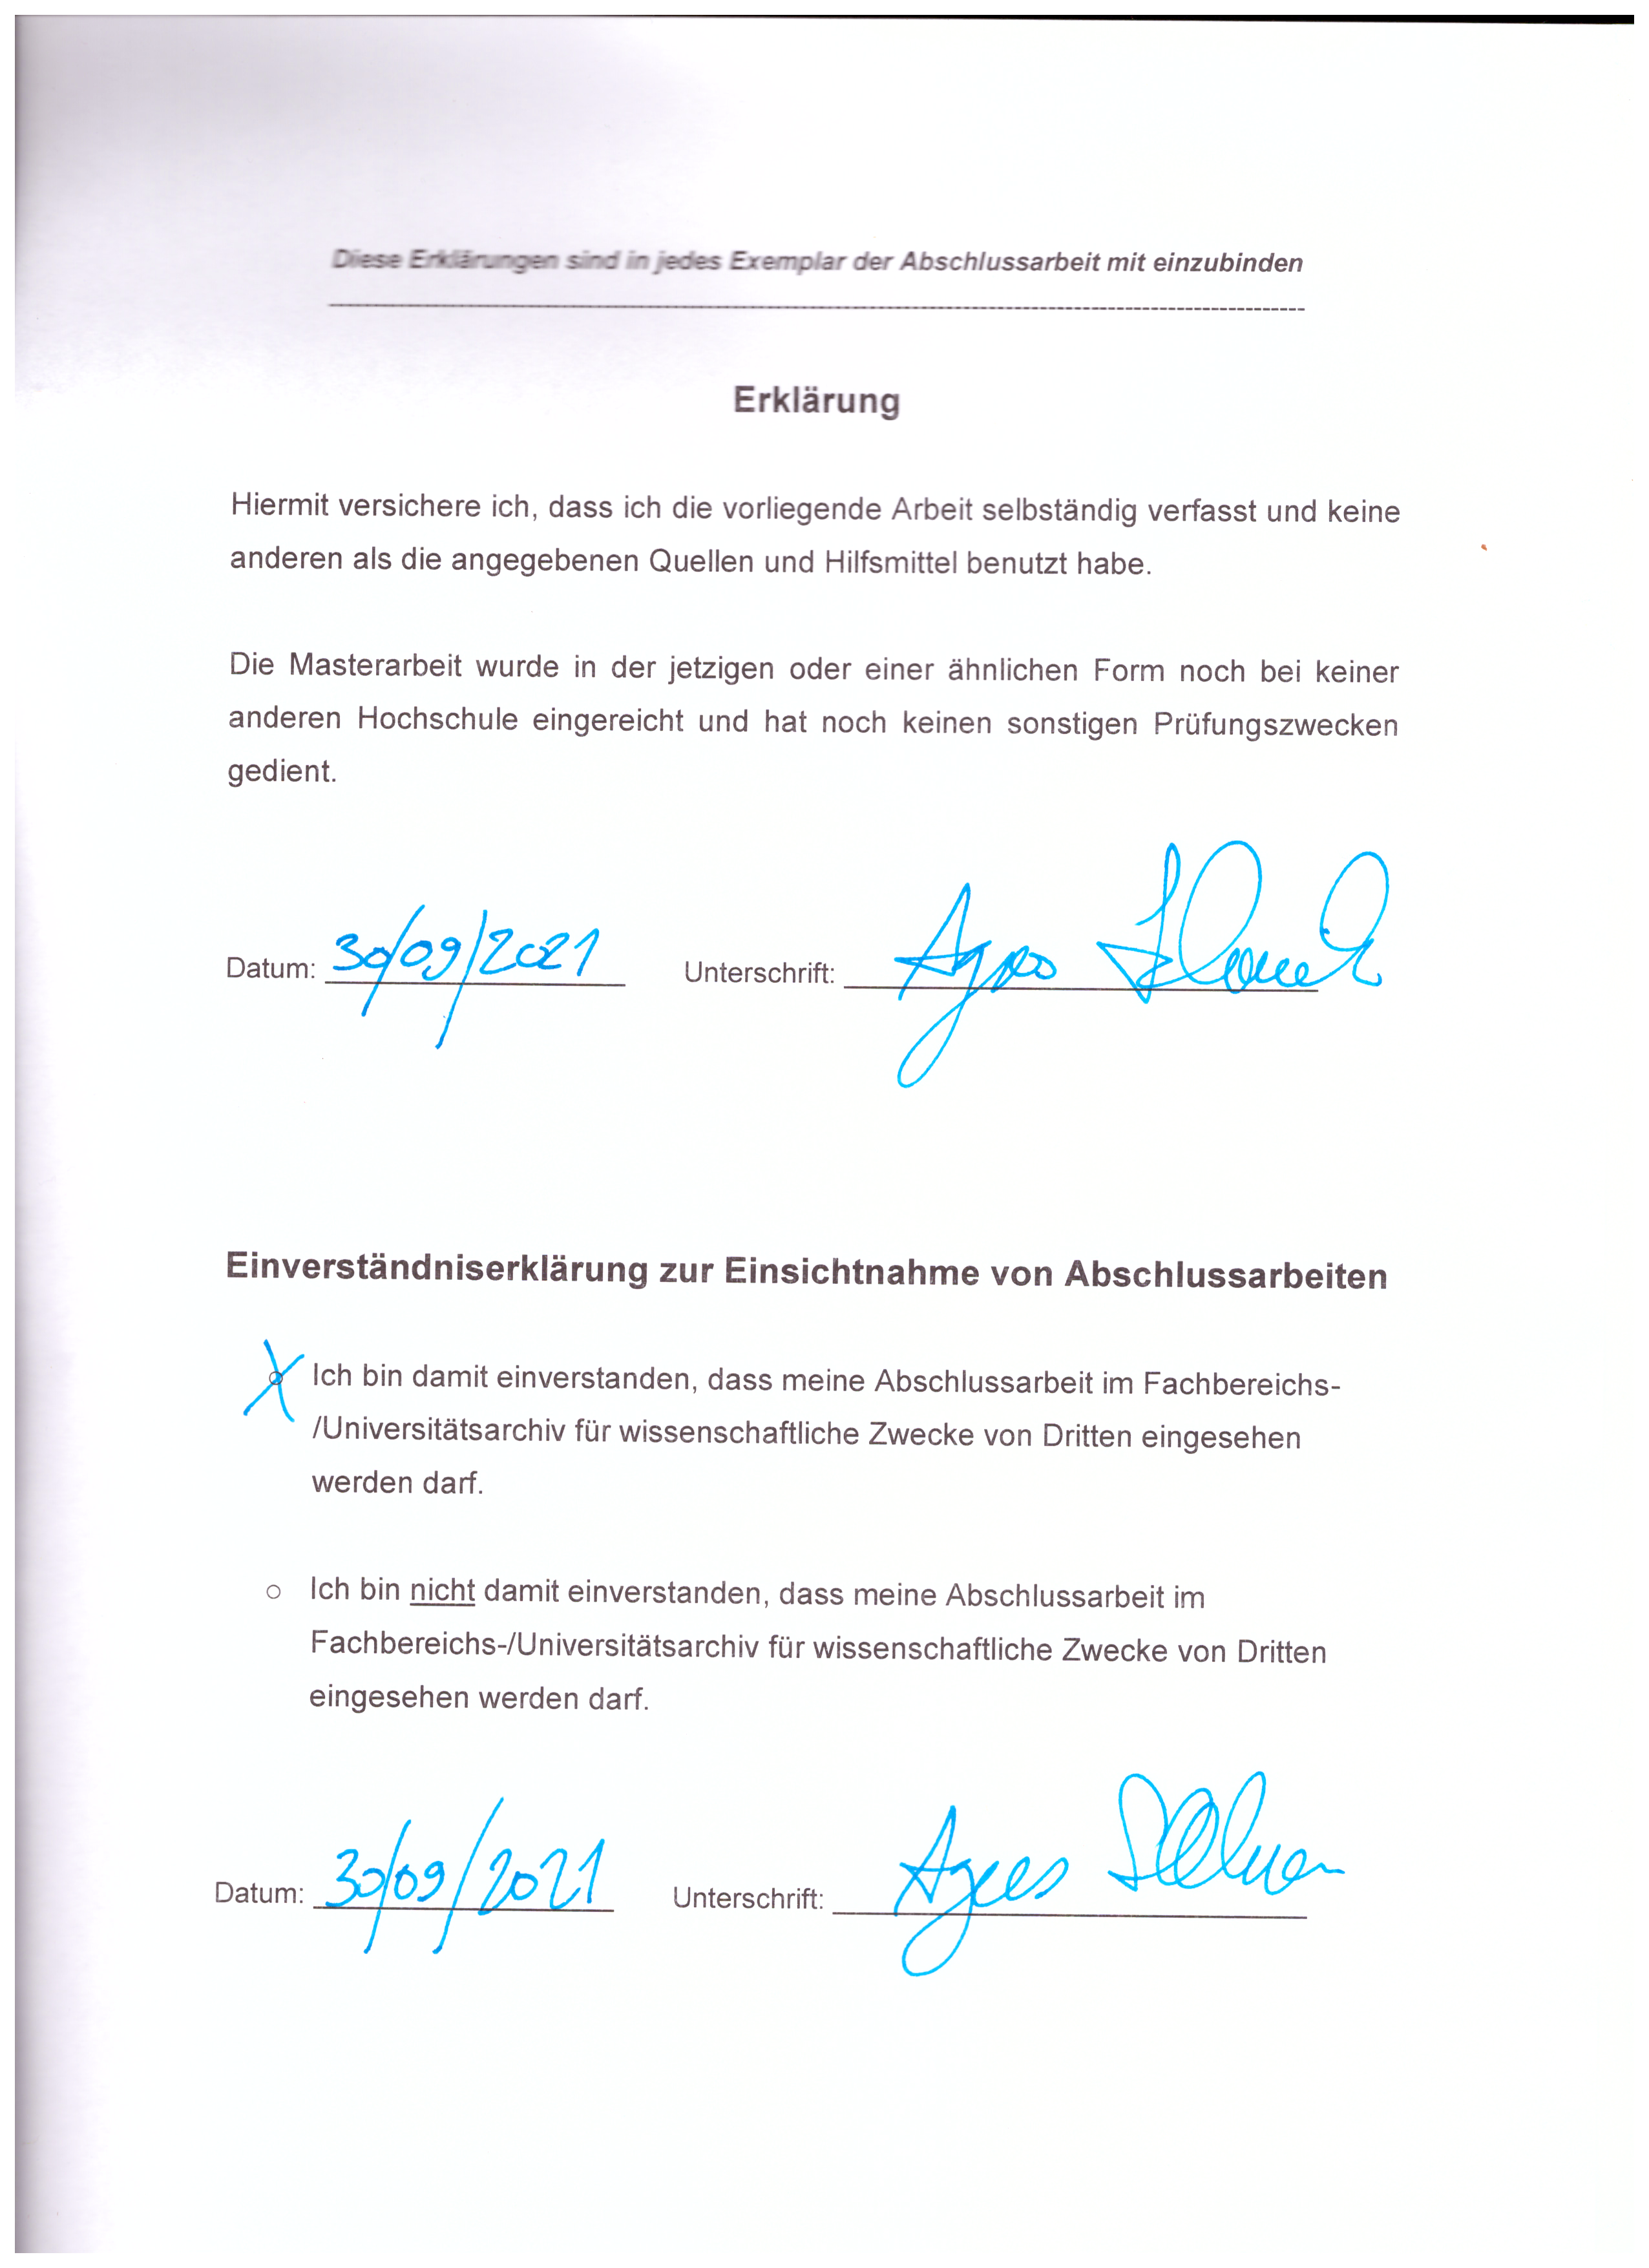
\includegraphics[width=1\linewidth,height=1\textheight]{C:/Users/kelto/Documents/iSEGMound/analysis/thesis/figures/Eigenstaendigkeitserklaerung} 

}

\end{figure}

\newpage
\vspace{1 cm}
\begin{centering}

\bf Abstract

\end{centering}

\vspace{1 cm}

This Master's thesis presents a workflow for (semi-)automated burial mound detection in LiDAR derived DEMs and their derivatives.
\newline
The thesis consists of two main sections. The first section starts with a discussion of Automated Archaeological Remote Sensing and its reception and perception in Archaeological Science, followed by the analysis of all published studies which have the aim to detect burial mounds or mound-like structures and are discussed in terms of used methods, software, accessibility of code and data. Then the toolbox for the thesis, a research compendium, to implement the \emph{desiderata} and requirements is discussed.
The second section start with the presentation of the case study area and the generalized workflow for automated analysis based on the studies discussed in the first section. This generalized workflow is the framework for the second part of the Master's thesis. As data-preprocessing step the generation of the used DTM from .LAZ file is explained and discussed, then as data preparation step different derivatives are calculated, explained and discussed and the \textbf{\emph{Multi-Scale Topographic Index (MSTPI)}} is chosen as an alternative for a \textbf{DTM/Hillshade} for the workflow. Next, the used data analysis methods and workflows used as precedents are discussed (the most accessible workflow is \textbf{iMound} and the only one reproducible workflow is published and developed in \texttt{R} is Niculita 2020, a GeOBIA workflow). Then the created \textbf{iSEGMound Workflow} for this thesis, based on the nature and condition of the geomorphology of the case study area, is detailed and explained. Afterwards, the best workflow of various alternatives with different data preparation methods (\textbf{\emph{DTM}} or \textbf{\emph{MSTPI}}) and data analysis methods (\textbf{Watershed Segmentation} or \textbf{Region Growing Segmentation}) is chosen using the IoU/Jaccrad Index. Subsequently the results of the \textbf{iSEGMound Workflow} on the case study area is advanced, only to discuss and evaluate it in the last chapter.
\newline
This thesis propagates a highly adaptable workflow, which elements can be extracted and used independently.

\newpage

\centering
\raggedright
\newpage
\tableofcontents

\newpage

\vspace{5mm}
\justifying

\hypertarget{preamble}{%
\section*{Preamble}\label{preamble}}
\addcontentsline{toc}{section}{Preamble}

Although this Master's thesis aspires to be as reproducible as possible in the form of a reproducible Research Compendium, hosted on Github, unfortunately the data set itself, on which the workflow is based, is not openly accessible. Although the Geography Department of the Philipps-Universität Marburg can use the LiDAR data for teaching purposes, it cannot be published anywhere.
On the other hand, it is possible to request the data set \href{Hessische\%20Verwaltung\%20für\%20Bodenmanagement\%20und\%20Geoinformation}{Hessische Verwaltung für Bodenmanagement und Geoinformation}. The following LAZ files were used:

\textbf{Train DTM:} 3dm\_32482\_5618\_1\_he.laz
\newline
\textbf{Train Area:} 3dm\_32482\_5616\_1\_he.laz, 3dm\_32482\_5617\_1\_he.laz,
\newline
3dm\_32482\_5618\_1\_he.laz, 3dm\_32482\_5619\_1\_he.laz, 3dm\_32483\_5616\_1\_he.laz
\newline
\textbf{Area of Interest 1:} 3dm\_32480\_5630\_1\_he.laz, 3dm\_32480\_5631\_1\_he.laz,
\newline
3dm\_32480\_5632\_1\_he.laz, 3dm\_32480\_5633\_1\_he.laz, 3dm\_32481\_5630\_1\_he.laz,
\newline
3dm\_32481\_5631\_1\_he.laz, 3dm\_32481\_5632\_1\_he.laz
\newline
\textbf{Area of Interest 2:} 3dm\_32484\_5630\_1\_he.laz, 3dm\_32485\_5630\_1\_he.laz,
\newline
3dm\_32485\_5631\_1\_he.laz, 3dm\_32485\_5632\_1\_he.laz, 3dm\_32486\_5630\_1\_he.laz,
\newline
3dm\_32486\_5631\_1\_he.laz, 3dm\_32486\_5632\_1\_he.laz
\newline
\textbf{Area of Interest 3:} 3dm\_32484\_5625\_1\_he.laz, 3dm\_32485\_5623\_1\_he.laz,
\newline
3dm\_32485\_5624\_1\_he.laz, 3dm\_32485\_5625\_1\_he.laz, 3dm\_32485\_5626\_1\_he.laz,
\newline
3dm\_32486\_5623\_1\_he.laz, 3dm\_32486\_5624\_1\_he.laz,3dm\_32486\_5625\_1\_he.laz,
\newline
3dm\_32486\_5626\_1\_he.laz, 3dm\_32486\_5627\_1\_he.laz, 3dm\_32487\_5626\_1\_he.laz,
\newline
3dm\_32487\_5627\_1\_he.laz, 3dm\_32487\_5628\_1\_he.laz
\newline
\textbf{Area of Interest 4:} 3dm\_32480\_5617\_1\_he.laz, 3dm\_32481\_5616\_1\_he.laz,
\newline
3dm\_32481\_5617\_1\_he.laz, 3dm\_32481\_5618\_1\_he.laz, 3dm\_32482\_5616\_1\_he.laz,
\newline
3dm\_32482\_5617\_1\_he.laz, 3dm\_32482\_5618\_1\_he.laz, 3dm\_32482\_5619\_1\_he.laz,
\newline
3dm\_32482\_5620\_1\_he.laz, 3dm\_32483\_5616\_1\_he.laz, 3dm\_32483\_5618\_1\_he.laz,
\newline
3dm\_32483\_5619\_1\_he.laz, 3dm\_32483\_5620\_1\_he.laz, 3dm\_32484\_5618\_1\_he.laz,
\newline
3dm\_32484\_5620\_1\_he.laz, 3dm\_32484\_5621\_1\_he.laz, 3dm\_32485\_5620\_1\_he.laz,
\newline
3dm\_32485\_5621\_1\_he.laz
\newline
\textbf{Area of Interest 5:} 3dm\_32478\_5624\_1\_he.laz, 3dm\_32479\_5624\_1\_he.laz,
\newline
3dm\_32480\_5624\_1\_he.laz, 3dm\_32481\_5624\_1\_he.laz

The code for the workflow and the Thesis itself (in multiple parts because the Supplement is too big) can be found on \href{https://github.com/keltoskytoi/iSEGMound}{Github:}

\newpage

\vspace{5mm}
\justifying

\hypertarget{acknowlegements}{%
\section*{Acknowlegements}\label{acknowlegements}}
\addcontentsline{toc}{section}{Acknowlegements}

The analysis of Automated Analysis Methods in Archaeological Remote Sensing was inspired by Irmela Herzog, who invited me in 2019 to the 24th CHNT (Cultural Heritage and New Technologies) in Vienna to talk about my then research (Pixel-based Image Analysis) where I heard among others the presentations on which Rom \emph{et al.} (2020), Kazimi \emph{et al.} (2019a) and Meyer \emph{et al.} (2019) is based. These manifold directions lead me to the survey part of this thesis, to understand what has been done and how until now. This idea was enforced by the Machine Learning in Archaeology Conference held in Rome (subsequently after CHNT 24), where I heard the research on which Orengo \emph{et al.} (2020), Trier \emph{et al.} (2021) is based and many more inspiring talks and ideas.
\newline
The idea of reproducible research - as far as I was able to fulfill the aim in this Master's Thesis - was fueled by publications and R packages of Ben Marwick and my participation at several Sessions of the CAA SIG SSLA (Scientific Scripting Languages in Archaeology) since it's foundation in 2018. I would like to thank Oliver Nakoinz, who has encouraged me in 2018 after my EAA presentation to go further on the path of Quantitative Archaeology and reproducible practice.
\newline
Further several colleague, scholars and friends must be named, who inspired me with their questions or critique or their work. First I would like to thank the whole Geography Department in Marburg, which put up with my special ideas and questions all the time, not being a Geographer. I would like to thank Chris Reudenbach who opened for me the world of R and Computational Modelling and who's on point critiques made me want to be more precise and to understand this new world better and better.
I met quite a few scholars on my visits to AARG, CAA and other conferences, but also online platforms are during Corona great for making connections with other scientists - having the same or similar problems, like different groups on Slack - this way I met Maria Elena Castiello whom I have to thank for the perfect Rumsfeld citation. Here I also met Sophie Schmidt who helped me to get started with an .Rmd. fitting for a thesis and not only a report. At this place I would also like to thank Luise Wraase and Simon Seyfried, who read Chapters 1 to 3 and gave useful advice.
\newline
There are many whom I want to thank because they inspired me one way or the other but the space should be filled with the thesis and not my ramblings. Speaking of ramblings - which is a saying of Rog Palmer: this way I am also thanking him for always keeping me on my toes about AI and Machine Learning - you are right, I am detecting here only round things, I saved the other objects for my Doctoral Dissertation.
\newline
Penultimate but not less importantly I would like to thank Karsten Lambers, who took it upon himself to be second supervisor to this thesis and was scholarly, patient and compassionate about my situation of having already a job and still finishing up this thesis.
\newline
At last but not least I would like to thank my family: my parents and Róbert who endured the silent times when I was roaming on scientific grounds.
\newline
Without all of you, I couldn't have finished this thesis.

\newpage
\pagenumbering{arabic}

\vspace{5mm}
\justifying

\hypertarget{introduction}{%
\section{Introduction}\label{introduction}}

The use of quantitative methods in archaeology reach back to the end of the 19th century, but it was only after the middle of the 20th century that they became computer-based. The first applications of statistical-mathematical methods using computers revolutionized the handling of spatial and quantitative archaeological data (e.g. Goldmann (1979)) and also the view on archaeology itself (e.g. Clarke (1968) and almost a decade later Hodder \& Orton (1976), Ihm \& Zimmermann (1978) to begin with). This quantitative analytical view preceded and prepared archaeologists for the advent of the public availability of soon high resolution digital data sets which revolutionized and broadened Aerial Archaeology, drawing upon the expertise of Satellite Remote Sensing and branching into a new discipline: Archaeological Remote Sensing. These new data sources, including geophysical platforms, led to the need to handle - in archaeological terms - big spatial data, thus to the specialized use of GIS platforms and the development and application of new methods like predictive modelling (Leusen \& Kamermans (2005); Kamermans \emph{et al.} (2009)). The sophistication of airborne platforms, sensors and imaging technologies, like LiDAR, hyper-spectral imagery and drone derived multispectral and hyper-spectral imagery (Agapiou \& Lysandrou (2015); Luo \emph{et al.} (2019)) facilitated the diversification of the toolset of Archaeological Remote Sensing.
New technical developments continuously push specialists to look for, borrow and adapt new methods to analyse in archaeological sense big data, which first lead to automating tasks such as georeferencing or applying the same function on multiple rasters (Raun \& Petersen (2018), 70). Soon this lead to more complex automation -- that is automating whole workflows and also analysis.
Thus in contrast to other disciplines, Archaeological Remote Sensing and Archaeological Science itself was quite late in adopting and applying automated methods and thus, Automated Archaeological Remote Sensing is still in its infancy (Opitz \& Herrmann (2018), 30). Although accordingly, the expression `automated analysis' is still controversial, it is nonetheless used throughout this Master's thesis. It has to be emphasized that `automation' does not stand for completely automated workflows. It was chosen as a short phrase to address workflows with at least partly -- or mostly -- automated elements, because no one advocates `automatic archaeology' (Cowley (2012) and Cowley \emph{et al.} (2013), 6). Automated analysis, often also called semi-automated analysis, `simply' means that a part, often a major part of a specific workflow, is automated, meaning computer aided.
Critical voices about predictive modelling in GIS ˗ which can be seen as the precursor and actual starting point of automated analysis ˗ were very fittingly summarized by Wheatley (2004): predictive modelling is dehumanising, anti-historical and substitutes human actions with mathematical equations Wheatley (2004)). This distrust is reflected in the criticism towards automated analysis methods in the Archaeological and Archaeological Remote Sensing community, claiming, that archaeological projects are always locally specialized (Parcak (2019), 120) and that there is no generalized automation method that can be used location independently, which can locate atypical archaeological objects without producing a quite large miss-rate (Casana (2014), Casana (2020), S93). Taking these points into account: why only use one type of automated analysis method (Davis (2020a), 5)? Large-scale landscapes feature lots of different landscape forms and archaeological features which need to be addressed in different ways. It is evident that it is not possible to detect everything with one analysis method or algorithm, due to the variability of the archaeological record. Other considerations include reflections on Automated Archaeological Remote Sensing detecting round and square shapes over and over and when it will move to something more useful that actually resembles archaeological objects (Rog Palmer in personal discussion and several AARGnews Editorials and contributions, e.g.~AARGnews 62, 61)?
It is also somehow self-evident, that although pre-trained and known object classes are going to be detected, new and unexpected and also not detected objects always have to be expected. Thus expecting to detect unexpected or unknown object classes with supervised learning/automation is misleading and completely unrealistic (see a similar discussion about the use of predictive modelling in Wheatley (2004), 3.2.3). It is a fatal move to expect automation to be the magic trick, when it is not: it should be more seen as an extension of the archaeologist's toolbox. Because automated analysis is not to replace manual data evaluation which, based on the personal experience of the operator and them being human, can be prone to missing knowledge or error, or even archaeologists completely, but to be complementary. Automated analysis should be followed by field observation and identification for assessment, which on the other hand also can be biased for the same reason as manual data evaluation (Cowley (2012), Bennett \emph{et al.} (2014), 899). All in all automated analysis is to ease and facilitate the amount of work archaeologists are facing with the increasing amount of data and different data types to analyse and evaluate. As Davis (2020b), 3 emphasizes: automated analysis is precise and manual analysis is accurate. Thus both methods combined can help archaeologists to penetrate a hidden level of any data set and landscape, which is invisible or hardly visible even for the trained eye.
Taking it further, reproducible analysis (Marwick (2017), Rokem \emph{et al.} (2017), Marwick \emph{et al.} (2018), Calero Valdez (2020)) can help to facilitate automated analyses and can serve as control for human individuality: because archaeologists do see different things in the same data set and unconsciously see what they are familiar with and what they know (Cowley (2012) 7), very similarly to an algorithm trained to find a certain class of object. Human detection cannot be reproduced but automated analysis can: via documented, reproducible workflows. In order to achieve this goal open-source scripting languages like R, Python or open-source platforms like Google Engine should be used, to be able to repeat, reproduce and even replicate workflows to facilitate their use by other scholars. When writing code, the semantic syntax has to be clear and consistent. This also makes sure that the ontology and the semantic syntax will be the same when the code is used by a different operator on a different dataset -- in contrary to manual analysis, where independent, subjective manual operators would define features or objects differently -- thus arriving to the same or a least similar bias and errors, of course depending on the dataset. This argument is investigated more thoroughly in chapter 3 and the expressions reproducible and replicable are discussed in more detail.

Being entirely different disciplines, there is a semantic gap between the ontologies of Computer Vision, Image Analysis and Remote Sensing on one hand and Archaeology on the other hand -- especially because the archaeological record itself is fragmented, multifaceted and poses ontological problems in itself for the interoperability of projects or databases, conducted by different operators with possible different metalanguage. Although the aim of this thesis is not the creation of an ontological and semantic framework and/or a metalanguage for Automated Archaeological Remote Sensing, these points have to be discussed because they affect the way how automation can be harmonized with Archaeological Remote Sensing.\\
This fundamental difference is reflected in the fact, that a distinction has to be made between `object' and `feature' in \emph{sensu stricto} automation, based on \emph{termini technici} from Computer Vision, on which ground `object' is referred to real-world entities in remote sensing images and `feature' to elements of an image and of an object (Traviglia \emph{et al.} (2016), 12; and Lambers \emph{et al.} (2019), 2), in contrary to the every-day use of the expression `archaeological feature' at an excavation site or in reports. Reproducible code and workflows enable to conduct the same `procedure' in a controlled environment and thus possible semantic problems which can result from how different operators see archaeological objects and features can be detected, distinguished and solved. Thus the accurate expert knowledge of manual analysis can be integrated in the precision and consistency of computational semantics (Davis (2020b), Fig 1.).

\begin{figure}

{\centering 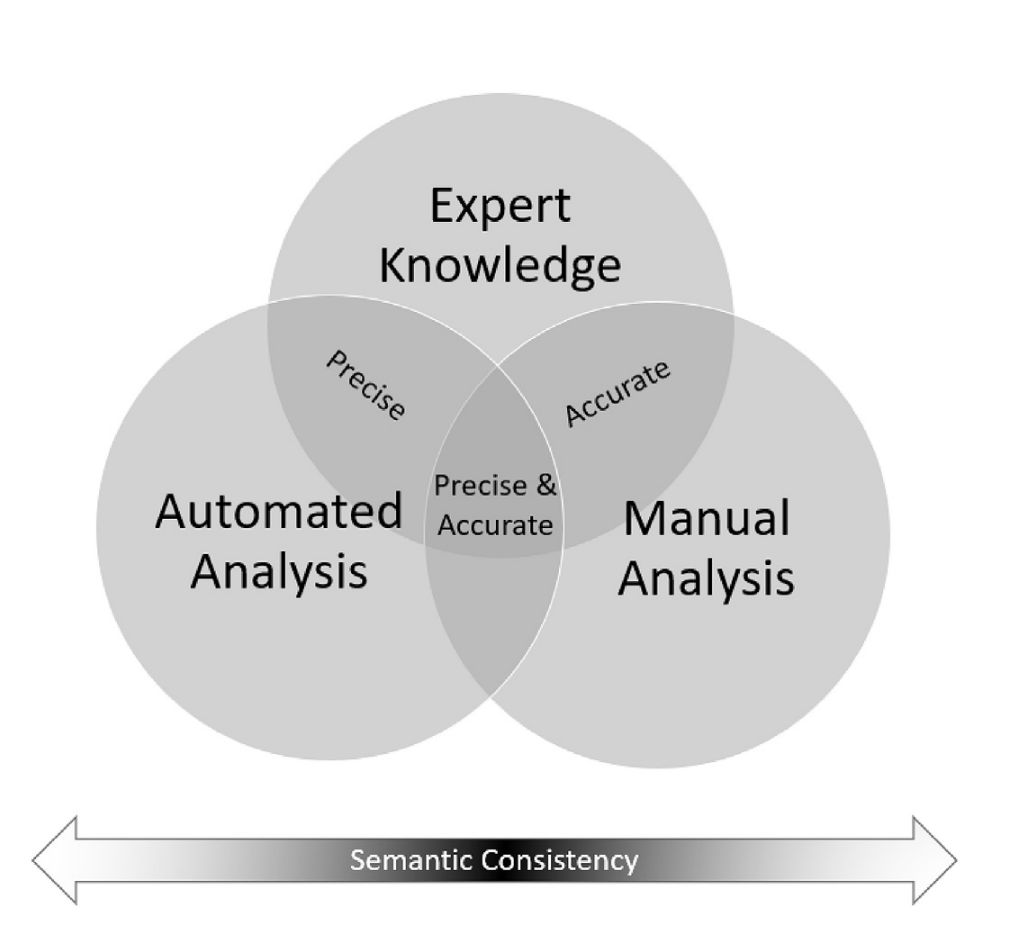
\includegraphics[width=0.5\linewidth,height=0.5\textheight]{C:/Users/kelto/Documents/iSEGMound/analysis/thesis/figures/Figure_1} 

}

\caption{Chart showing the advantages (approaching Semantic Consistency) when Expert Knowledge, Manual Analysis and Automated analysis are combined. Source: Davis 2020a, Fig 1.}\label{fig:Figure1}
\end{figure}

On the other hand, manual analysis can learn a lot from the systematic precision of reproducible code: defining variables, consistent nomenclature of objects/ forms/ features; creating functions: setting the relation of objects/ forms/ features. This needs the consistency of formalized, straightforward and clear definitions (also Magnini \& Bettineschi (2019), 13, Davis (2020b)). Thus ontology, semantics and metadata are very important tools which enable us to connect and share code, databases and research. By shared ontologies (knowledge representation), codified metalanguage protocols and rule-sets, not only would the transferability of expert knowledge be substantially eased between Archaeological disciplines and Automated Archaeological Remote Sensing, but also between its different sub disciplines, like Template Matching-, Geometric knowledge-, GeOBIA-, Machine Learning- based analyses (this distinction is explained in chapter 2).

So then, after all, how to semantically address the varying, unpredictable, fragmented, multifaceted and diachronic archaeological record (monuments and artefacts) which can be detected in remote sensing data with methods of Computer Vision and Image Analysis? Remote sensing data offers much more: they are diachronic time capsules, records of palimpsest landscapes, archaeological, micro- and macro-topographical, geomorphological and also recent, anthropomorphic traces (Magnini \& Bettineschi (2019), 12) in a multidimensional space. Thus a common ground has to be created (a shared diachronic formalized ontology) to fill the semantic gap between the metalanguage of human perception, the archaeological record (which is manifold, imbalanced and changing in time (conceptually and physically) and Computer Vision/Image Analysis. And a way has to be found to apply this new diachronic formalized ontology onto real world scenarios (using Automated Archaeological Remote Sensing). Real world (archaeological) scenarios are often extremely complex and thus robust simplification and formalization has to be executed to break down complexity and bring the domains in discussion together. Sevara \& Pregesbauer (2014) already pioneered a conceptual framework in 2014, which found resonance and the formulation of a Diachronic Semantic Model (DSM) in Magnini \& Bettineschi (2019), which was successfully applied by the latter on a case study in 2021 (Magnini \& Bettineschi (2021)). These fundamental studies are the first steps towards integrating Automated Archaeological Remote Sensing in the nervous system of Archaeological Science.

As concluding thoughts let a quote from Quintus \emph{et al.} (2017) 1 state: \emph{``many archaeological professionals who might have an interest in lidar-derived products do not have the technical experience to modify or create AFE (automated feature extraction) techniques for particular regions or environments.''} This should not impact the scientific methods one chooses. With open-source, reproducible (regularly updated and version controlled) and code, with clear replicable workflows and published data and study (at least the manuscript in a pre-print repository) (Figure 3), every remote sensing archaeological professional should be able to tap into the possibilities of Automated Analysis. Thus open access and open source software should be used, training data sets and workflows released to be able to learn from each other and to progress, building on the experience of each other and not to have to start from scratch with every new project conducted.

\begin{figure}

{\centering 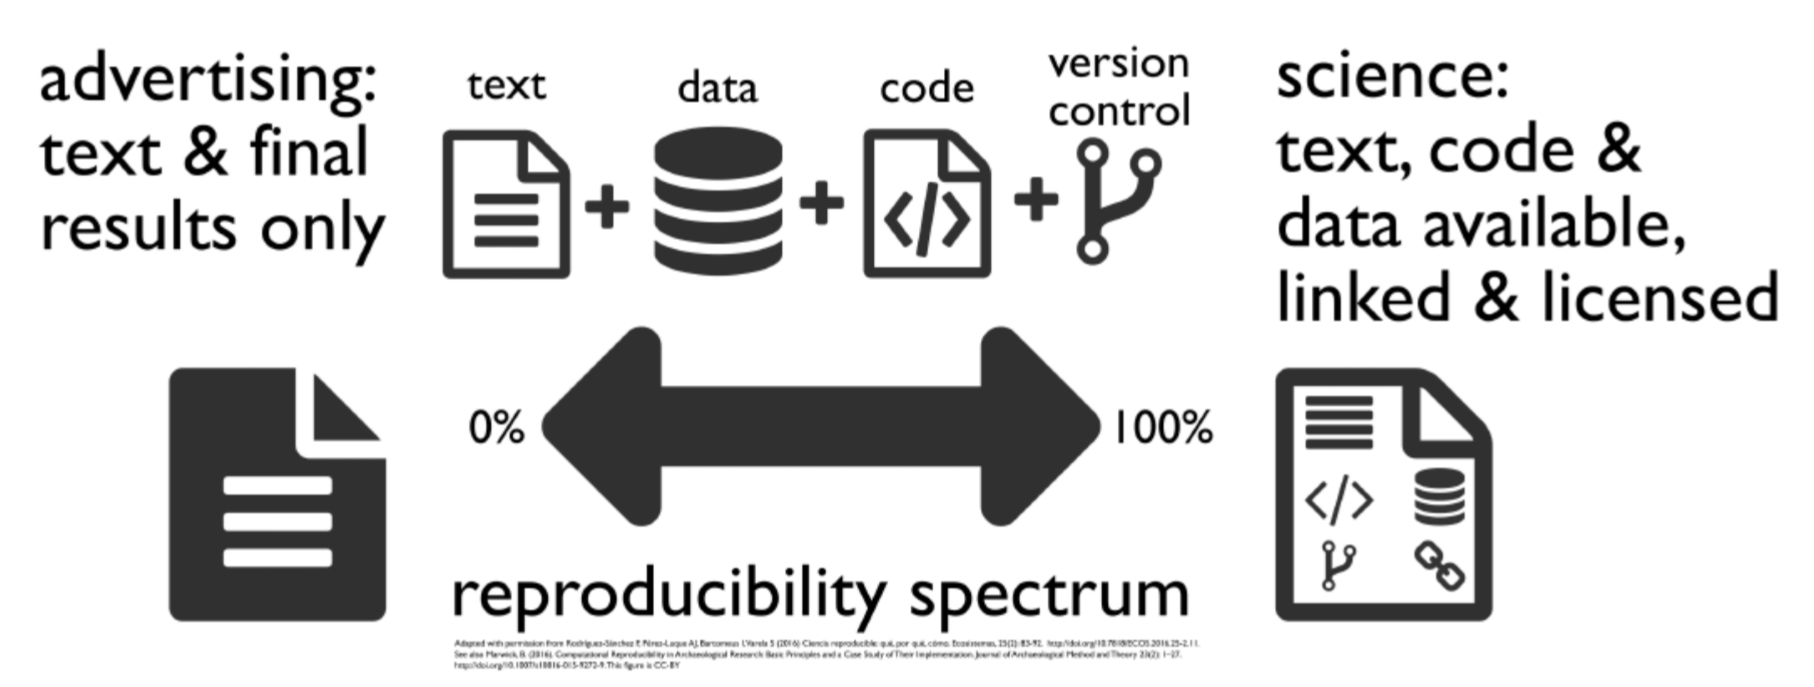
\includegraphics[width=0.75\linewidth,height=0.75\textheight]{C:/Users/kelto/Documents/iSEGMound/analysis/thesis/figures/Figure_2} 

}

\caption{The difference between articles behind paywall and reproducible (and replicable) studies. Source: Marwick et al. 2017, Figure 1.}\label{fig:Figure2}
\end{figure}

Thus we not only need to compare the accuracy and the true and false positive rate of different automated methods (Trier \emph{et al.} (2019), Table 1) and the methods themselves (Davis \emph{et al.} (2019)), but we need to make a compendium of these methods with the key elements mentioned above. Combined with this, a baseline or best practice for the different methods should be defined that can be utilized by beginners. Thus open-access code, workflow and protocol, published (at least training) data sets and best practices are needed as reference and base line for other studies, stored in an open-source database or platform which can support open-source computer languages.

Different observations made above and questions based on these have led to the objective of this thesis. Firstly: based on scientific literature, on what grounds lies the dispute of automation in Archaeological Remote Sensing and how can it be relieved? Is the experience and knowledge gained transferable to other studies? How many scientific studies on burial mound detection worked transparently and retraceable (reproducible if not replicable) in any step of their workflow? Can experiences and knowledge from previous studies be used to create a reproducible and replicable workflow for burial mound detection?\\
Thus the aim of this Master's thesis is to emphasize the applicability and usefulness of automation in dealing with big data sets in Archaeological Remote Sensing and the need for reproducible and replicable workflows and studies. The case study for this thesis is the detection of burial mounds in LiDAR data sets in R, to substantiate this point of view.

To approach these questions accordingly, after the discussion of Automated Archaeological Remote Sensing and its reception in Archaeological Science was discussed in Chapter I, the Introduction. In the next chapter (2) all published studies whose goal is to detect burial mounds or mound-like structures are discussed in terms of used methods, software, accessibility of code and data. It is also elaborated why burial mounds are chosen as Objects of Interest and which methods will be applied and why. Chapter 3 provides the toolbox for the thesis to implement the \emph{desiderata} and requirements discussed in Chapter 1 and 2. Chapter 4 presents a reproducible workflow for the detection of burial mounds in LiDAR data. Chapter 5 (Results), Chapter 6 (Discussion) and Chapter 7 (Conclusion) completes the endeavour of this Master's thesis.

\newpage

\vspace{5mm}
\justifying

\hypertarget{exploitation-of-automated-analysis-methods-to-detect-burial-mounds-and-structurally-similar-archaeological-objects-a-survey}{%
\section{Exploitation of Automated Analysis Methods to detect burial mounds and structurally similar archaeological objects: a survey}\label{exploitation-of-automated-analysis-methods-to-detect-burial-mounds-and-structurally-similar-archaeological-objects-a-survey}}

The analysis carried out and communicated in this chapter reviews all published studies which are aimed at the detection of burial mound and mound-like structures in order to define a baseline to place present research. Numerous reviews of methods and applications used in Archaeological Remote Sensing have been carried out (e.g. Leisz (2013), Agapiou \& Lysandrou (2015); Davis (2019), Luo \emph{et al.} (2019), Fiorucci \emph{et al.} (2020)): some broad and general, some more specific. The word survey was chosen specifically, because it was not a systematic search of databases as various `classical' reviews did (such as Agapiou \& Lysandrou (2015), Raun \& Petersen (2018), Magnini \& Bettineschi (2019) and Davis (2020a) and Davis (2020b)).
This survey is building on the experience of aforementioned systematic reviews (which show very diversified nomenclature and heterogeneous terms) and the scientific literature was collected based on these reviews, Researchgate, Academia and mainly considering open-access publications (if possible). As a starting point all published studies (at least available to the author via University access; number of studies in August 2021: 96) have been collected which deal with the automation of Archaeological Remote Sensing data set (practical studies which use any automation methods and analysis) but only those are discussed, which are concerned with the detection of burial mounds and structurally similar archaeological objects: altogether 31 publications. Burial mounds have been chosen as Objects of Interest for the review because they are relatively simple structures and a very common funerary custom throughout human history. Similarly structured archaeological objects like tell mounds or other monumental earthworks of circular form can be found in very different areas and time periods and are widely investigated and thus deliver good examples of automated analysis methods of these archaeological objects. The first archaeological objects to automatically detect were tell mounds and only then and with the dawn of the use of LiDAR data came burial mounds into the focus of research. While the early research carried on tell settlements can be connected to Ur \& Menze, the monumental earthworks and mound shell rings can also be allocated to two research groups: Freeland et al.~and Davis, Lipo \& Sanger. The detection of burial mounds themselves shows more variability in the investigators (Figure 3). A complete list of references (which is by far not conclusive and is to be supplemented) is included as a supplement at the end of this thesis (Supplement 1).

\begin{figure}

{\centering 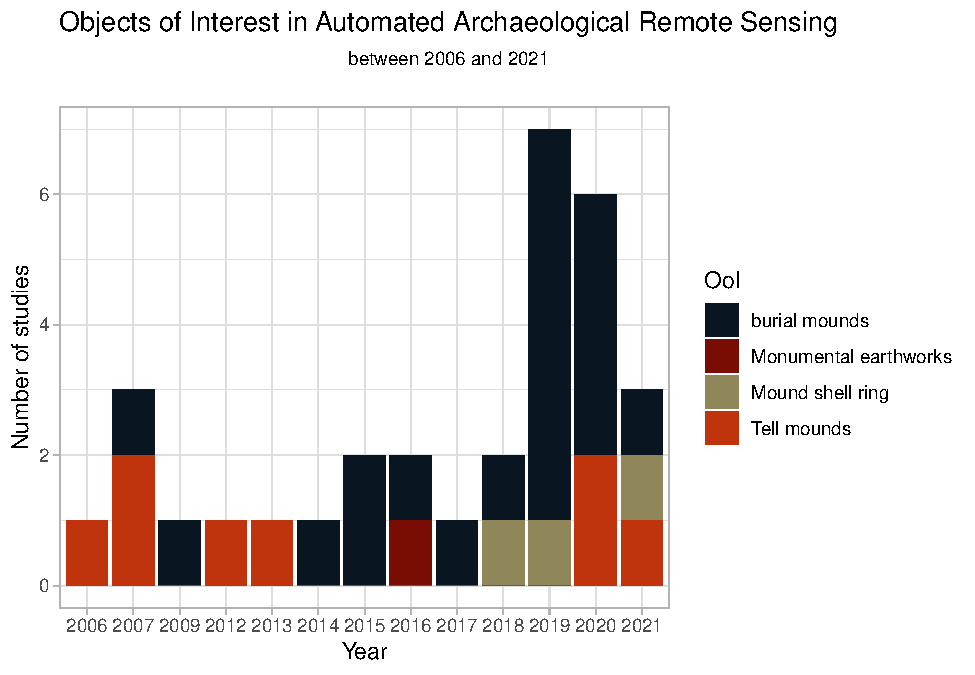
\includegraphics{Index_files/figure-latex/Figure3-1} 

}

\caption{The Objects of Interests investigated by year between 2006 and 2021.}\label{fig:Figure3}
\end{figure}

The main points considered in this survey were chosen based on the aforementioned reviews, which were conducted looking at citation indexes of different Remote Sensing methods in scientific periodicals (Agapiou \& Lysandrou (2015), Raun \& Petersen (2018), Luo \emph{et al.} (2019), Davis 2020b), Institutional Affiliations of researchers (Agapiou \& Lysandrou (2015), Raun \& Petersen (2018)), the citation network (Raun \& Petersen (2018)), OBIA by geographic region (Davis (2019)), the developments and limitations of OBIA methods (Davis (2019)), research goal using OBIA (Davis (2019)), the development of different passive and active Remote Sensing methods (Luo \emph{et al.} (2019)), the scale of ArchaeOBIA applications (Magnini \& Bettineschi (2019)), datasets and methods applied in Archaeological Remote Sensing (Fiorucci \emph{et al.} (2020)), different parameters, thresholds, methods and accuracy used in the automated detection of mound features (Davis (2020b)) and geometric disparity of Remote Sensing methods Davis (2020a)).
These systematic reviews stimulated questions such as: How can we learn from previous studies? How transparent is the workflow and if described, which variables and parameters (rule sets) were used? Which software was used? How reproducible or even replicable is the workflow in the studies?

Based on these questions the points investigated in this Master's thesis are (Supplement 1):

\begin{enumerate}
\def\labelenumi{(\roman{enumi})}
\tightlist
\item
  Location (only in Supplement 1)
\item
  RS (Remote Sensing) data
\item
  Methods
\item
  Detail of methods (only in Supplement 1)
\item
  Variables/morphometric parameters
\item
  OoI (Objects of Interest)
\item
  Scale
\item
  Software
\item
  Access
\end{enumerate}

The point ``Location'' (i) was documented, because different geographical and landscape conditions ask for different methods and objects can appear geographically and culturally diverse, which can explain the chosen method. The point ``RS data'' (ii) documents which type of remote sensing data was used and also it's resolution if known. The point ``Methods'' (iii) organizes the studies in five main categories (Template Matching, Geometric Knowledge-based, GeOBIA-based and Machine Learning-based, Deep Learning; see Figure 4), based on Cheng \& Han (2016) (also see Lambers \emph{et al.} (2019) and Roffler (2020)), instead of juxtaposing pixel-based and object-based methods. This differentiation points out the different object detection methods based on the approach to the dataset. Still, for the differentiation of Machine Learning-based methods, the expression pixel-based is going to be used for the classifier training-based methods, also because several studies use it (Sevara \emph{et al.} (2016), Niculiță (2020b)).

\begin{figure}

{\centering 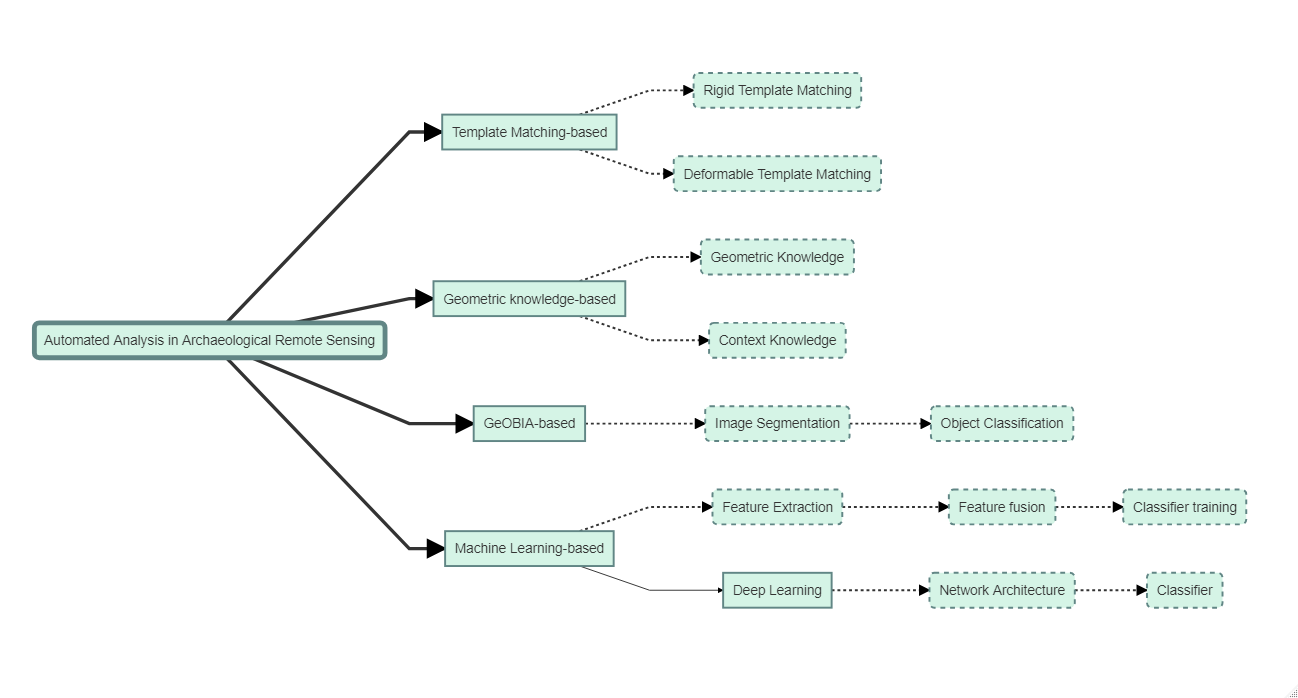
\includegraphics[width=1\linewidth,height=1\textheight]{C:/Users/kelto/Documents/iSEGMound/analysis/thesis/figures/Figure_4} 

}

\caption{Taxonomy of Automated Analysis in Archaeological Remote Sensing, based on Cheng and Han 2016.}\label{fig:Figure4}
\end{figure}

The point ``Details of method'' (iv) explains the workflow of the study in a nutshell, if comprehensible. Point v, ``Variables/Morphometric parameters'' highlights the variables and or morphometric parameters used in the study. ``OOI'' (vi) are the objects investigated. The point ``Scale'' (vii) implies the geographical range of the study, if it was applied to a broader region than the area on which the method was developed. The last two points (``Software'' - viii, and ``Access'' - ix) investigated give us hints about the accessibility of the dataset and the code. Especially in earlier studies, information about the software used is not mentioned and sometimes can only be guessed. In the case of ``Access'', apart from the information about accessible data and code it was also documented if there is a workflow (a comprehensible sequence of the steps of the workflow) or a flowchart (a very generalized workflow without clear steps) or if any of the equations used was published and or explained. It was also documented if any supplementary information or document was attached to the study which can guide to a better understanding for a possible reproduction of the study. Although all these points have been investigated, for practical reasons mainly the points (ii) RS (Remote Sensing) data, (iii) Method/s, (iv) Detail of method/s, (v) Variables/morphometric parameters, (vi) OoI/Object(s) of Interest, (viii) Software and (ix) Access is going to be elaborated in depth in this and the next chapter.

It is essential to discuss the basic traits of the used methods (iii, Supplement 2) in short, concentrating on their application in Archaeological Remote Sensing. It has to be stressed, that still no semantic \emph{lingua franca} (between Archaeological Remote Sensing and Computer Vision and Remote Sensing Methods) exists when talking about automated methods in Archaeological Remote Sensing, thus methods are addressed in different ways (or most commonly in a very simplified way) and it is not always possible to determine which exact method has been utilised (recently it is improving, but it depends where the authors put the focus of their work). First, when shortly discussing the basic traits of the methods and their use in Archaeological Remote Sensing, it is only focused on the use of the different methods (what is used, where and when) since 2006, when tell mounds were first investigated using automated analysis methods. In the second part of this chapter the way of their use is investigated and analysed how the methods are used.

\textbf{\emph{Template Matching-based methods}} utilize a template of the Object of Interest to be detected, which is then statistically matched to the input image. Two general directions can be distinguished: Rigid Template Matching, which requires a precise template which gets problematic when it comes to intra-class shape and size variations. Deformable Template Matching on the other hand can handle either free-form deformable templates or parametric deformable templates. (Cheng \& Han (2016), 13-14).
In the literature investigated Template Matching was used seven times for the detection of burial mounds, mound shell rings and tell mounds (Boer (2010), Kramer (2015), Trier \emph{et al.} (2015), Davis \emph{et al.} (2018), Raun (2019), Davis (2019), GholamReza \& Malian (2021)). Apart from Kramer (2015), Rigid Template Matching was preferred (Supplement 2). Template Matching itself is a method which is being revisited from time to time (Figure 5).

\begin{verbatim}
## [1] "Year"   "Method" "Freq"
\end{verbatim}

\begin{figure}

{\centering 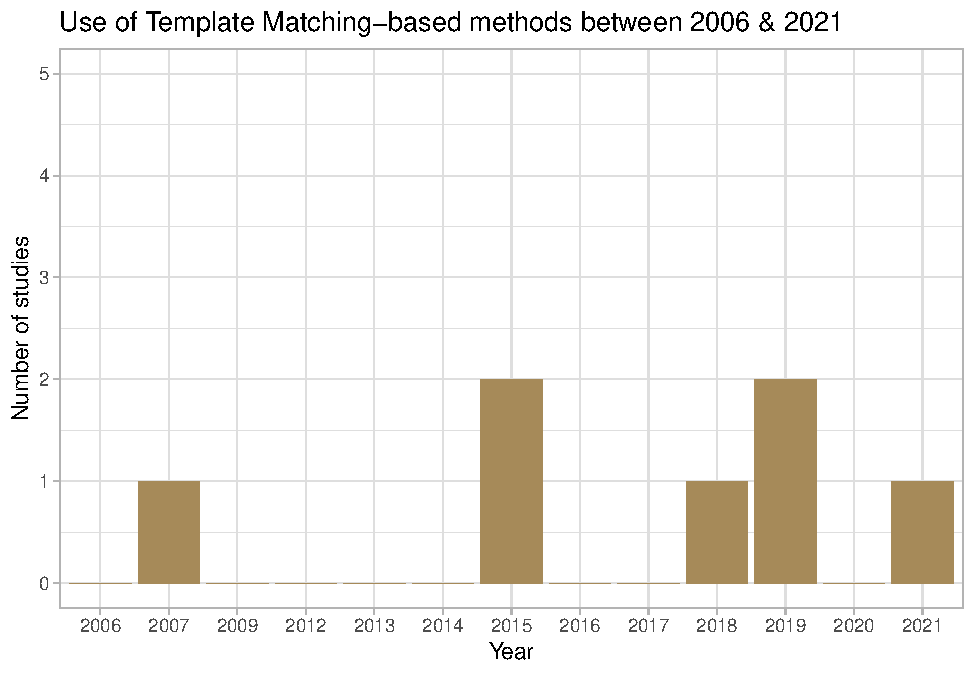
\includegraphics[width=0.75\linewidth,height=0.75\textheight]{Index_files/figure-latex/Figure5-1} 

}

\caption{The Objects of Interests investigated by year between 2006 and 2021.}\label{fig:Figure5}
\end{figure}

\textbf{\emph{Geometric knowledge-based analysis}} works with specialized solutions for specific problems, applying rules based and established on knowledge of the regions of interest and it's context. It uses either encoded prior geometric knowledge of the generic specificity of the Object of Interest and then e.g.~applies hand-crafted mathematical morphometry rules for object extraction (morphometric derivatives such as Slope, Aspect, Curvature, Local Relief Model, vegetation indices etc.). Context knowledge based analysis uses knowledge about the relationship of the Object of Interest and the area it should be separated from (e.g.~filters, textural analysis) (Cheng \& Han (2016), 15). In the case of Automated Archeological Remote Sensing the two Geometric knowledge-based analysis approaches are often used in combination and form the data preparation step (Figure 6). Geometric knowledge based object analysis is only occasionally used per se as an automated analysis method for the detection of burial mounds, monumental earthworks and tell mounds: Riley (2009), Freeland \emph{et al.} (2016), Rom \emph{et al.} (2020). (Lately) it is only occasional, that Geometric knowledge-based object analysis is not used as data preparation method (Boer (2010), Caspari \emph{et al.} (2014), Trier \emph{et al.} (2015), Raun (2019), Caspari \& Crespo (2019), Kazimi \emph{et al.} (2019b), Kazimi \emph{et al.} (2019a)). In some cases, Geometric knowledge based analysis is included in the future work (compare works by Kazimi \emph{et al.} (2019a) vs. Kazimi \emph{et al.} (2020))(Supplement 2).

\begin{verbatim}
## [1] "Year"   "Method" "Freq"
\end{verbatim}

\begin{figure}

{\centering 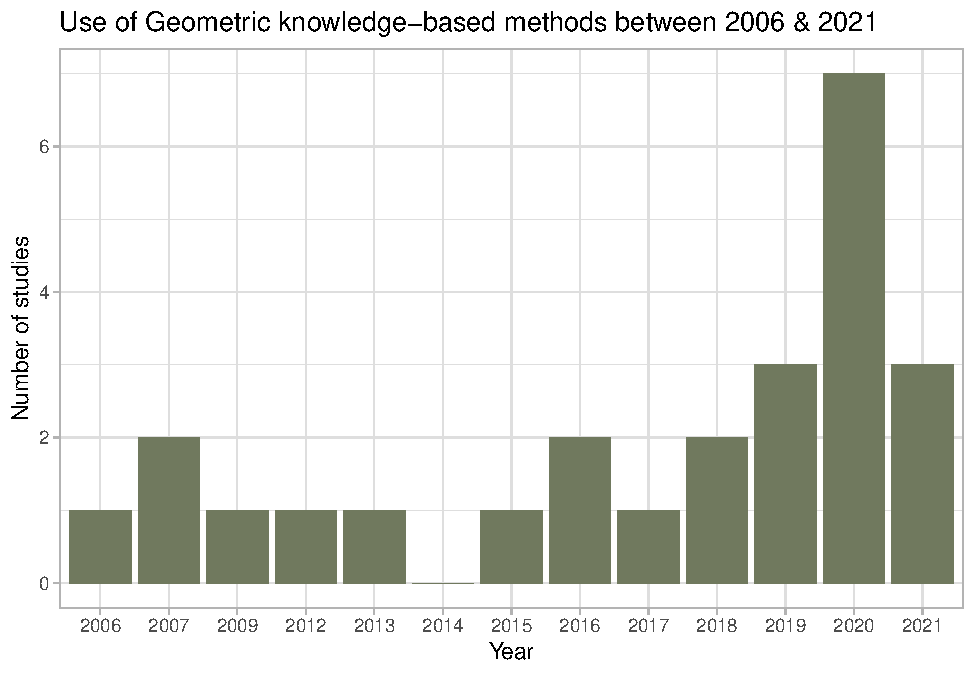
\includegraphics[width=0.75\linewidth,height=0.75\textheight]{Index_files/figure-latex/Figure6-1} 

}

\caption{The use of Geometric knowledge-based methods distributed by year between 2006 and 2021.}\label{fig:Figure6}
\end{figure}

\textbf{\emph{Geographical Object-based Image Analysis (GeOBIA)}} dates back to the late 1970's (Blaschke \emph{et al.} (2014)), but it was only around 2000 that Object-based Images Analysis became widely used in Remote Sensing studies due to the availability of high resolution Satellite data. This induced a paradigm shift not only in Remote Sensing but generally in GI Science, hence its new name: GeOBIA (Hay \& Castilla (2008)). GeOBIA operates in two steps: images are divided into small segments, which are defined by the homogeneity of specific morphometric (shape, size, orientation), spectral, textural, context and neighborhood parameters (Hay \& Castilla (2008)) and are then grouped together to meaningful homogeneous object candidates (the segmentation step), which are then classified by specific extracted object criteria in question (the feature extraction and classification step, Blaschke \emph{et al.} (2014), 186, Cheng \& Han (2016), 15, Hossain \& Chen (2019), 115) or filtered by a rule-set. Various types of segmentation methods exist (as also their categorization: Blaschke (2010), Blaschke \emph{et al.} (2014), Kumar \&.R (2014)). Lately Hossain \& Chen (2019) investigated the different segmentation methods from a Remote Sensing point of view, but here only the two main Segmentation methods used in Automated Archaeological Remote Sensing studies are described: Watershed Segmentation (or Transformation) (Niculiță (2020a) and Niculiță (2020b)) and Multiresolution Segmentation (Kramer (2015), Sevara \emph{et al.} (2016), Freeland \emph{et al.} (2016), Davis \emph{et al.} (2018) and Davis \emph{et al.} (2019), Meyer \emph{et al.} (2019), Sărășan \emph{et al.} (2020)), the first being an Edge-Based Segmentation method, the latter a Region-Based Segmentation method. For an in-depth analysis of the methods see Hossain \& Chen (2019).

\emph{Edge-Based Segmentation techniques} are `top-down' methods: first they locate edges in the image and then use contouring algorithms to close them. Edges are regarded as boundaries between objects where pixel properties are abruptly changing (Hossain \& Chen (2019), 117). `Watershed Segmentation' (implemented in open source software e.g.~in SAGA or in the ForestTools package in R) simulates real-life flooding. It first transforms the image into a gradient (grey-scale), then identifies objects with clear segment boundaries, only to then create (fill) objects, for which it is also called a Region-Growing algorithm (Hossain \& Chen (2019), 117, Table 1; Figure 7).

\begin{figure}

{\centering 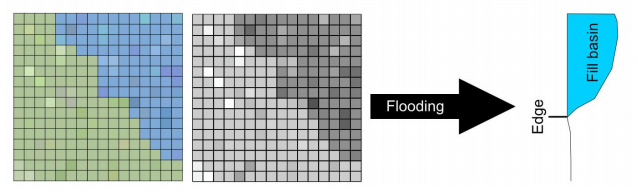
\includegraphics[width=8.86in]{C:/Users/kelto/Documents/iSEGMound/analysis/thesis/figures/Figure_7} 

}

\caption{Operating principle of ‘Watershed Segmentation’. Roffler 2020, 33.}\label{fig:Figure7}
\end{figure}

Region-Based Segmentation techniques start from the complete opposite: they begin with an initial segmentation of the whole image (thus also called `bottom-up methods') based on a specific rule-set. Regions are generated in two completely different ways: either by splitting the image into homogeneous regions based on inhomogeneity (region-splitting and then merging) or by region-growing from a so-called seed-region based on homogeneity (region-growing and then merging, Hossain \& Chen (2019)). `Multiresolution Segmentation' (Baatz \& Schäpe (2000), for which mainly eCognition is used in Automated Archaeological Remote Sensing) is a region-merging hierarchical segmentation method which starts with one pixel (seed) and applies pairwise merging of segments to build up hierarchical levels. The merging -- or clustering (using local rule sets) is repeated (on multiple levels), until an object is recognized (Hossain \& Chen (2019), 119, Roffler (2020), 33-34; Figure 8).

\begin{figure}

{\centering 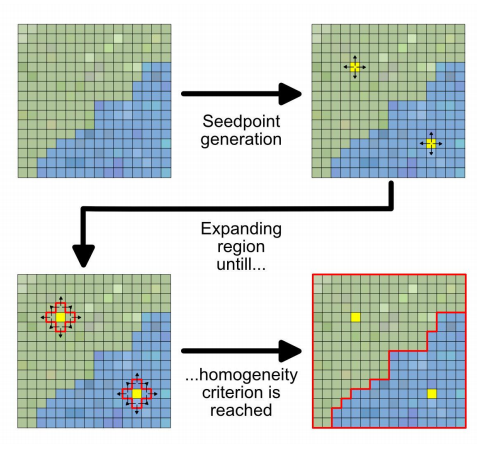
\includegraphics[width=0.75\linewidth,height=0.75\textheight]{C:/Users/kelto/Documents/iSEGMound/analysis/thesis/figures/Figure_8} 

}

\caption{Operating principle of ‘Region Growing Segmentation’. Roffler 2020, 34.}\label{fig:Figure8}
\end{figure}

With regard to (Automated) Archaeological Remote Sensing, GeOBIA is sometimes also called archaeOBIA (Lamotte \& MASSON (2016)), which points to the fact, that (Automated) Archaeological Remote Sensing is in need of a completely different semantic ontology and rule sets than which is needed for customary GeOBIA methods used in Remote Sensing. Still recently the challenge in Remote Sensing has been to define segmentation parameters/rule sets which can be transferred to other images (Cheng \& Han (2016), 16) -- something archeOBIA is also struggling with (see Table 1; note the different variables used in the different studies).
Burial mounds, monumental earthworks and mound shell rings have been investigated using GeOBIA methods nine times since 2015 (Figure 9). Apart from one case (Niculiță (2020a): Watershed Segmentation, carried out with SAGA in R), Multiresolution Segmentation was applied (Supplement 2), almost exclusively using eCognition, (former Definiens), a software developed for and with the evolution of GeOBIA and thus is generally considered ``the software'' for GeOBIA (Blaschke (2010), Fig 4, Hossain \& Chen (2019), Fig 1.), which is clearly reflected in this survey.

\begin{verbatim}
## [1] "Year"   "Method" "Freq"
\end{verbatim}

\begin{figure}

{\centering 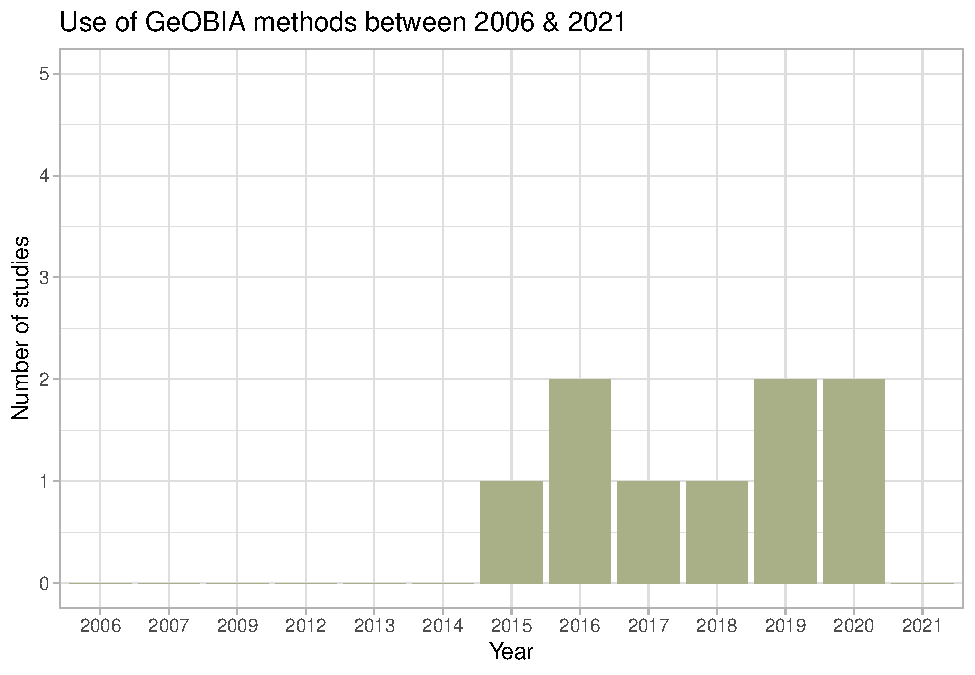
\includegraphics[width=0.75\linewidth,height=0.75\textheight]{Index_files/figure-latex/Figure9-1} 

}

\caption{The use of GeOBIA methods distributed by year between 2006 and 2021.}\label{fig:Figure9}
\end{figure}

\textbf{\emph{Machine Learning-based methods}} are considered a subfield of Artificial Intelligence. Machine learning automates statistical methods to learn from input data either supervised, unsupervised or semi-supervised. Automated Archaeological Remote Sensing mainly utilizes supervised methods.
\emph{Pixel-based Image Analysis}, an image classification method, has been developed in the early 1970s for the digital analysis of Landsat Multispectral Scanner Systems (Phiri \& Morgenroth (2017) 2017, 9) and is (still) widely distributed in Remote Sensing research, especially in land-use and land-cover classification. In contrast to GeOBIA, Pixel-based Image Analysis approaches an image on pixel basis, which are classified into different categories based on the information they carry (usually one variable). Given that the second step of GeOBIA can be a classification of the segmented image using variables of the image-objects best describing the Objects of Interest, GeOBIA is sometimes also seen as a form of Machine Learning (Davis (2019), 1).
Random forest classifiers are supervised learning algorithms which consist of an ensemble of decision trees. Each (unrelated) decision tree is trained using a random subset of the training data. Each of these trees will give a prediction for a data point. Then, the prediction of all decision trees is averaged by a majority vote to a final prediction (Figure 9). The independence of the different decision trees increases the accuracy of the prediction and also eliminates problems that can be caused by outliers in the data set and works also well with small data sets, because of the facts just explained. These effects can be enhanced by resampling techniques and parameter tuning (Kuhn \& Johnson (2013)).

\begin{figure}

{\centering 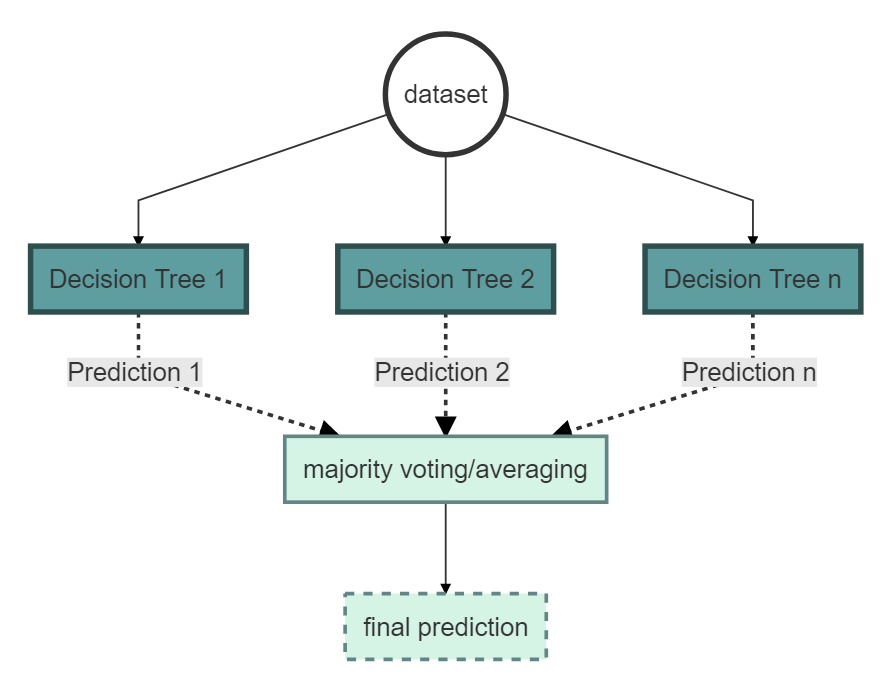
\includegraphics[width=0.5\linewidth,height=0.5\textheight]{C:/Users/kelto/Documents/iSEGMound/analysis/thesis/figures/Figure_10} 

}

\caption{Schematized modus operandi of the Random Forest algorithm.}\label{fig:Figure10}
\end{figure}

Regarding the automated detection of burial mounds and similar structures, Pixel-based classification was the first method used in 2006 and has been more or less revisited since (Figure 11). When looking closely at the specific algorithms used, it is not surprising why the Random Forest algorithm was exploited in most Pixel-based Image Analysis studies (Menze \emph{et al.} (2006), Menze \& Ur (2007), Menze \emph{et al.} (2007), Menze \& Ur (2012), and Menze \& Ur (2013), Kramer (2015), Guyot \emph{et al.} (2018), Orengo \emph{et al.} (2020), Niculiță (2020a), and Davis \emph{et al.} (2021)) and Mahalanobis Distance (Trier \emph{et al.} (2015) and Sevara \emph{et al.} (2016)) and Support Vector Machine Classifiers (Caspari \& Crespo (2019)) in less.

\begin{verbatim}
## [1] "Year"   "Method" "Freq"
\end{verbatim}

\begin{figure}

{\centering 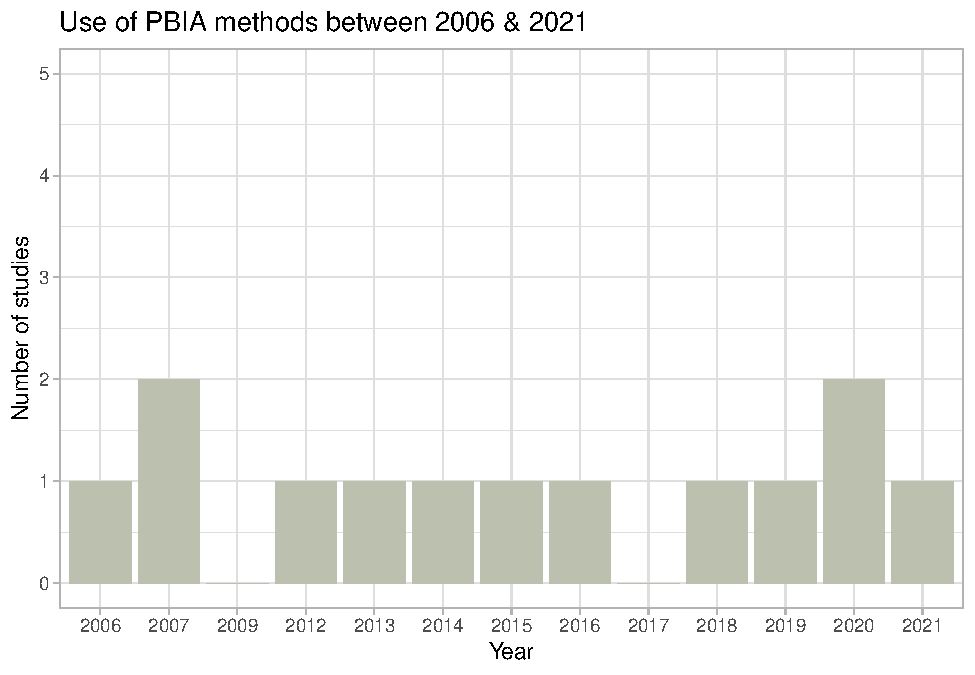
\includegraphics[width=0.75\linewidth,height=0.75\textheight]{Index_files/figure-latex/Figure11-1} 

}

\caption{The use of Pixel-based Image Analysis methods distributed by year between 2006 and 2021.}\label{fig:Figure11}
\end{figure}

It was already suggested that with the development of remote sensing sensors and resulting new, higher resolution datasets the need for new analysis methods is constantly stimulated. Starting with pixel-wise analysis and followed by the object-level addressing of remote sensing imagery, lately an even bigger semantic step was taken: the analysis on the scene-level, which can be seen as the next paradigm shift (Cheng \& Han (2016), Cheng \emph{et al.} (2020), 2, Fig. 2). The complex semantic structures of very high resolution images are addressed by \emph{Deep Learning}, which is also a sub-field of Machine Learning. In contrast to Pixel- and Object-based Image Analysis, Deep Learning Algorithms consist of multiple stacked hierarchical layers (network architectures) which can handle complexity and abstraction.
In the case of the identification of burial mounds and mound like structures Deep Learning is only in use since 2019 (Figure 12).

\begin{verbatim}
## [1] "Year"   "Method" "Freq"
\end{verbatim}

\begin{figure}

{\centering 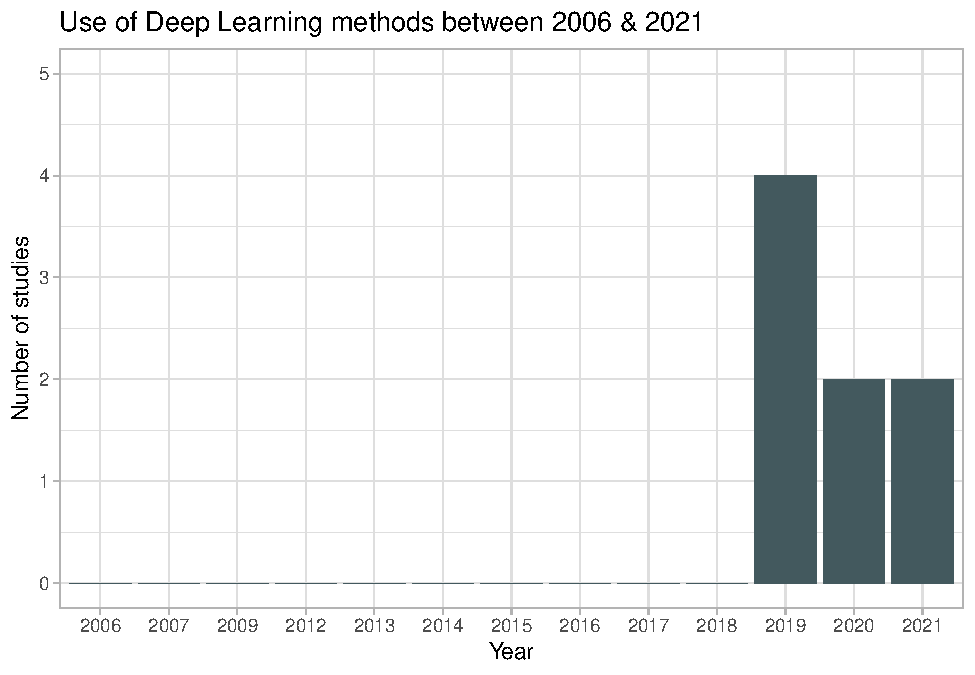
\includegraphics[width=0.75\linewidth,height=0.75\textheight]{Index_files/figure-latex/Figure12-1} 

}

\caption{The use of Deep Learning methods distributed by year between 2006 and 2021.}\label{fig:Figure12}
\end{figure}

To summarize the use of automated analysis methods to detect burial mounds and mound-like structures (Figure 13), it can be established that the first method used was Pixel-based Image analysis (Menze \emph{et al.} (2006)), followed by Template Matching (Boer (2010)). Geometric knowledge-based analysis was used as an autonomous method only by Riley (2009), Freeland \emph{et al.} (2016), Rom \emph{et al.} (2020), but as already concluded it is more often than not incorporated in workflows as data preparation method (e.g. Cerrillo-Cuenca (2017)). GeOBIA was first used in 2015 and remained a very effective analysis method, until recently when Deep Learning became widespread (including Semantic and Instance Segmentation).

\begin{figure}

{\centering 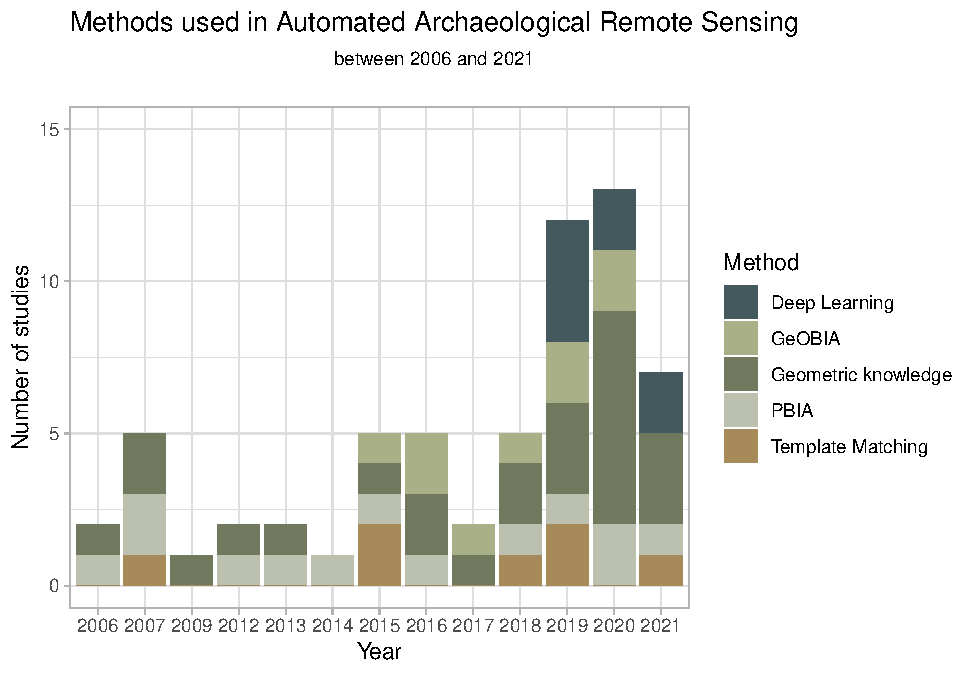
\includegraphics[width=0.75\linewidth,height=0.75\textheight]{Index_files/figure-latex/Figure13-1} 

}

\caption{The use of different Image Analysis methods to detect mounds and mound-like objects distributed by year between 2006 and 2021. Note: this represents the number of methods used, not the number of studies.}\label{fig:Figure13}
\end{figure}

Several studies compare different analysis methods or combine them. Freeland \emph{et al.} (2016) and Davis \emph{et al.} (2019) compare Geometric-knowledge-based analysis (iMound/Inverse Stochastic Depression Analysis) to GeOBIA, with success (this is also reflected in the fact that the original algorithm iMound by Freeland \emph{et al.} (2016) was reused by Davis \emph{et al.} (2019) and Rom \emph{et al.} (2020)). Template Matching has been compared to GeOBIA (Kramer (2015), Davis \emph{et al.} (2019): including Geometric knowledge-based method) and Pixel-based Image Analysis to GeOBIA (Sevara \emph{et al.} (2016)) and to Deep Learning (Caspari \& Crespo (2019)).

Although LiDAR data has been available for some time (see Boer (2010), Riley (2009)), it was only after 2010 that it made its way into everyday archaeological research, including various visualization methods (as Geometric knowledge-based analysis and data preparation method), making LiDAR visualisations a self-evident step for any archaeological project using ALS data (see also Kokalj \& Hesse (2017)). It is mainly from 2015, when ALS data started to dominate and revolutionize Automated Analysis methods in Archaeological Remote Sensing and provoking new approaches, such as GeOBIA (Figure 14). Since the diffusion of LiDAR data, Satellite Imagery is mainly used in large-scale studies (Caspari \& Crespo (2019) and Orengo \emph{et al.} (2020)). Studies which require high resolution data and utilize LiDAR quickly shifted to Deep Learning solutions. Simultaneously also UAV data finds its way into the general data repertoire of Automated Archaeological Analysis (Sărășan \emph{et al.} (2020)).

\begin{figure}

{\centering 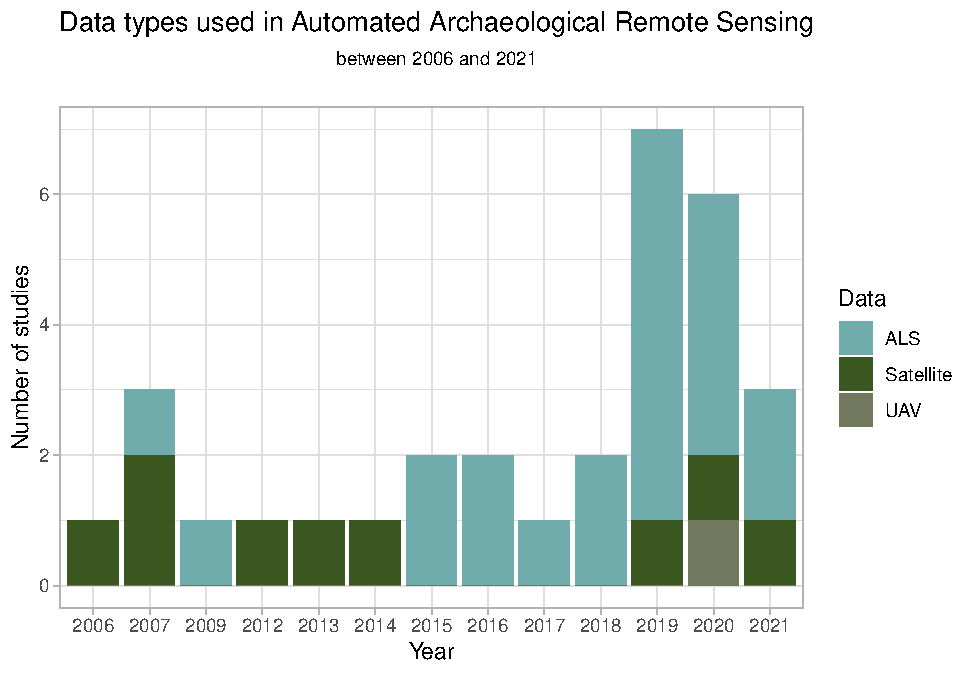
\includegraphics[width=0.75\linewidth,height=0.75\textheight]{Index_files/figure-latex/Figure14-1} 

}

\caption{The use of different data types used to detect mounds and mound-like objects distributed by year between 2006 and 2021.}\label{fig:Figure14}
\end{figure}

When taking the points `Software' and `Access' into account, it has to be expressed that it is only a recent phenomenon that software and computation details have to be disclosed when publishing a study. Even though lately many journals require data and code availability statements, only a few studies provide openly accessible code and data: Orengo \emph{et al.} (2020), and Niculiță (2020a). In the first case the data and the code are available using Google Earth Engine. In the latter case, the regulations of the local Cultural Heritage Management authorities require a signed form through the author of the study to be able to use the DEM on which the study was based on - nonetheless it can be accessed. Although with restrictions.
Inspecting the information about the methodology details of the studies, nine cases have been identified (Figure 15): from not available (n/a) to workflow \& code \& data, many constellations can be observed. In many cases the workflow was published, in some cases only a flowchart. In this thesis as a workflow the clear explanation of the methodology in a chart form is defined (with a big probability of reproducibility if the observer knew the exact tools and software used or if those were made clear). As a flowchart on the other hand, a part of a workflow or a very schematized workflow was identified where only the main steps were arranged in chart form, thus making it impossible to trace back the specific steps and to reproduce the workflow or any part of it. Thus the only reproducible study, which published a really detailed workflow, the code and made the data set - although restricted by certain rules - available is Niculiță 2020.

\begin{figure}

{\centering 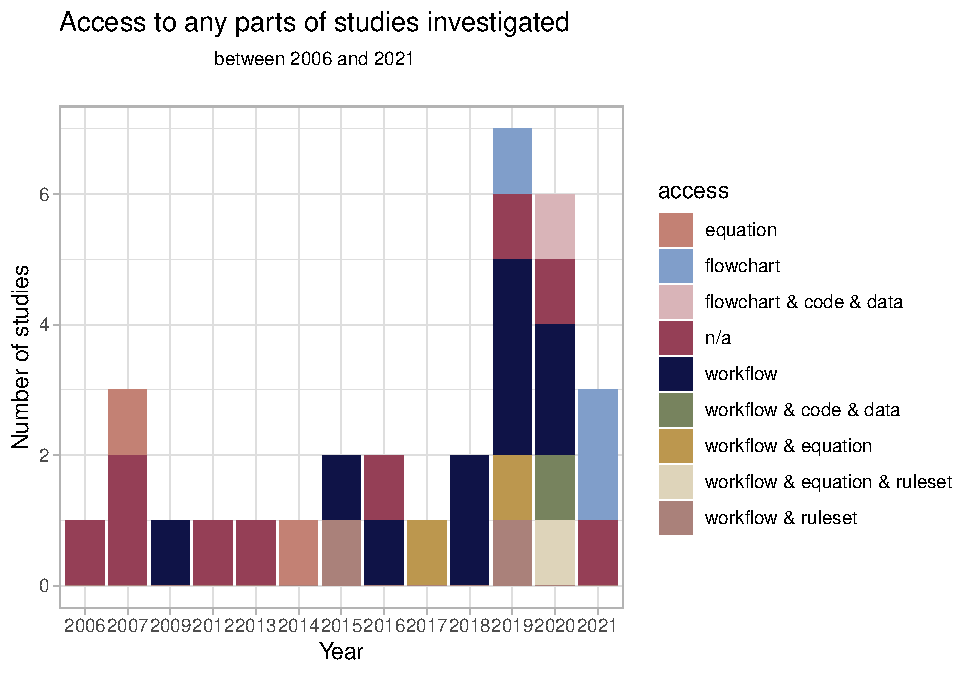
\includegraphics{Index_files/figure-latex/Figure15-1} 

}

\caption{Access to any parts of  studies used to detect mounds and mound-like objects distributed by year between 2006 and 2021.}\label{fig:Figure15}
\end{figure}

As already noted, eCognition is considered ``the'' software for GeOBIA (Hossain \& Chen (2019), 122) thus it is evident that many will choose this simpler solution. At the same time, it must be emphasized that the first analyses were carried out in R (Menze \emph{et al.} (2006), Menze \emph{et al.} (2007), Menze \& Ur (2007), Menze \& Ur (2012), and Menze \& Ur (2013)), i.e.~with open source software. Using proprietary software not only marginalizes researchers and institutions who/which can't afford rather expensive software, but it is also hard to comprehend the exact algorithm behind the software, and to understand to be able to apply it in another domain. It is also important to understand why certain tools or algorithms worked or did not work? This can only be done by creating reproducible workflows with open source software. In 2019 and 2020 more than 60\% of the studies were conducted with FOSS (Free and Open Source Software) software. This number is only increasing (Figure 16).

\begin{figure}

{\centering 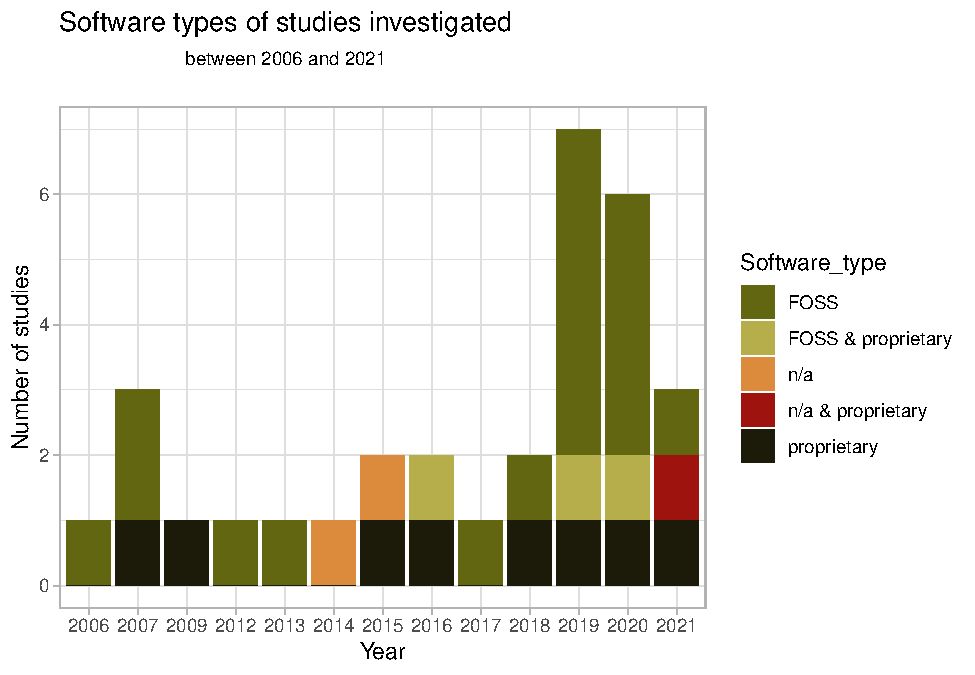
\includegraphics{Index_files/figure-latex/Figure16-1} 

}

\caption{Software types of studies used to detect mounds and mound-like objects distributed by year between 2006 and 2021.}\label{fig:Figure16}
\end{figure}

This survey served the purpose to elaborate the development of Automated Analysis in Archaeological Remote Sensing, mainly with regard to the applied methods, the used software and access to information about the workflow. The aim was to show how little reproducible research has been published with regard to automated analyses and how much there is to be done in the future. Also, automated analysis in Archaeological Remote Sensing is being carried out on different scales with different algorithms, specialized to different research questions in mainly research contexts. This is also a reason why many critical voices see automated analysis methods as pastimes and not really something operational (see many AARGnews Editorials). To give way for the next chapter we can conclude that the results of automated analyses are compelling, but many studies start basically from the beginning, because when research is published without accompanying software, workflow, data and documented steps, it is a challenge and time consuming to understand, verify, expand and eventually surpass that research (Marwick (2017), 425). This is one reason why many research projects start from the beginning, with a new idea instead of building on the previous knowledge. Another point is that automated analysis methods in Archaeological Remote Sensing are still in their infancy (Opitz \& Herrmann (2018) 2018, 30) and best practices have not yet been established. Nonetheless it has to be stated that automated analysis itself is not a goal, but a method, a means to an end to further research and thus reproducible or even replicable best practices would help shift the focus on further development of methods than on continuous recommencement.

Chapter 2 discussed the use of automated analysis methods in Archaeological Remote Sensing for the detection of burial mounds and structurally similar archaeological objects. It was demonstrated that only 2 out of 31 studies have disclosed workflow, code and data and are thus reproducible (see chapter 3 for explanation). As a reproducible study in the R environment Niculiță (2020a) can be mentioned as the best example. It was also noted that even without the availability of code, there are workflows which are illustrated and also explained clearly enough that they can be reproduced, which on the other hand can take some time but is still possible to do when having enough experience with spatial tools.
On this basis it was decided that the Geometric knowledge-based workflow `iMound' (established by Freeland \emph{et al.} (2016) and reused by Davis \emph{et al.} (2019) and Rom \emph{et al.} (2020)) is going to be utilized in R to detect burial mounds in LiDAR data in this Master's thesis to create a reproducible workflow. During the implementation of the workflow it became clear that on the basis of the geomorphometry of the Train Area it was necessary to include another method to be able to effectively detect burial mounds (this is discussed in depth in Chapter 4). Thus, in addition to `iMound' also parts of the reproducible workflow of Niculiță (2020a), a GeOBIA method was used in this Master's thesis.

\newpage

\vspace{5mm}
\justifying

\hypertarget{towards-a-paradigm-shift-in-archaeological-remote-sensing-practice-by-means-of-tool-driven-automated-analysis}{%
\section{Towards a Paradigm Shift in Archaeological Remote Sensing practice by means of Tool-driven Automated Analysis}\label{towards-a-paradigm-shift-in-archaeological-remote-sensing-practice-by-means-of-tool-driven-automated-analysis}}

In Chapter 2 the arguments of reproducibility and replicability have been addressed regarding the accessibility of data, code and workflow of the investigated studies. It was demonstrated that only 2 out of 31 studies have disclosed all three elements and are reproducible. It is important to discuss the exact definition of both expressions. In this Master's thesis mainly the definitions of Marwick (2017) are followed.
Reproducibility means that code and workflow of an analysis reproduces all results and figures in the respective publication from its original raw data. Replicability stands for the replication of the workflow (from data collection to data analysis) onto a new dataset. It was mentioned in the introduction that optimal reproducible open science would incorporate version controlled open code, clear workflows and open datasets or at least training datasets.

So then, how is the best way to implement and guarantee reproducibility? Marwick (2017) outlined four general principles of reproducible research:
i) Data and code provenance, sharing and archiving (analogue to artifact provenience)
ii) Scripted analyses (for reproducibility and ideally replicability)
iii) Version control (transparency of decision points of any research and possibility of collaboration)
iv) Self-contained computational environments (sharing the computational environment of the analysis for replicability).

Pushing forward along this road, Marwick \emph{et al.} (2018) propose R-packages as research compendia to organize transparent and reproducible research to approach the general principles laid out in 2017. Research compendia should organize files according to conventions: separate data, method and output (the latter being disposable because they can be reproduced) and define which exact computational environment was used for the analysis. Building an R package around a research project automatically forces one to keep the guidelines and conventions of package building which also provides quality control mechanisms.
Research compendia come in many forms and complexities, as Marwick \emph{et al.} (2018) discusses. The author of this Master's thesis experimented with a basic form of reproducible research compendium when analyzing the finds of an Iron Age cemetery in Hungary using multivariate statistical analysis (Schneider (2019b)). The work was done basically in an R project with a fixed project structure which was uploaded in a github repository (\url{https://github.com/keltoskytoi/Multivariate_Statistics_Szentloerinc}). The repository contains an .Rproj file with the settings for the project, a folder called DATA for the raw data to be analyzed and not to be changed during the study, two .R files with the code used for the analysis in the study, a README.md file with basic information of the paper, thus the title and where to get it. An earlier study and research compendium from 2015, but already in a very mature form by Ben Marwick already shows the many of the elements of an optimal research compendium (listed in Figure 12), organized as an R package with the published compendium on figshare for the study Clarkson \emph{et al.} (2015) which is also completely replicable: \url{https://github.com/benmarwick/1989-excavation-report-Madjedbebe}; \url{https://figshare.com/articles/software/1989_excavation_report_Madjebebe/1297059}
A recent use of a research compendium is Schmid 2019 with the compendium published at OSF. This study is also completely replicable:
(\url{https://github.com/nevrome/cultrans.bronzeageburials.article2019}, \url{https://osf.io/b6np2/})
Based on the reproducibility of these studies and on the personal experience and motivation mentioned above, it was decided to create a research compendium for the Master's thesis.

The optimal outline for a complex research compendium in an R environment is reproduced from Marwick \emph{et al.} (2018), Figure 4:

\begin{figure}

{\centering 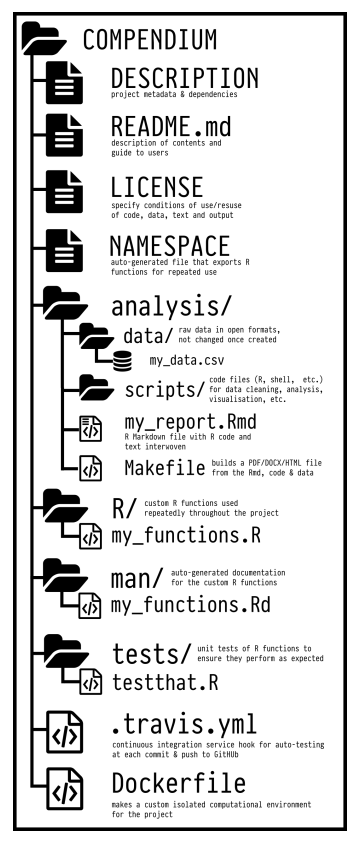
\includegraphics[width=0.5\linewidth,height=0.5\textheight]{C:/Users/kelto/Documents/iSEGMound/analysis/thesis/figures/Figure_17} 

}

\caption{Schematized modus operandi of the Random Forest algorithm.}\label{fig:Figure17}
\end{figure}

This optimal research compendium outline is implemented in the R package rrtools (`reproducible research tools', \url{https://github.com/benmarwick/rrtools}) by Ben Marwick, which helps to write reproducible research papers, setting up the structure propagated in Marwick \emph{et al.} (2018). Although this Master's thesis cannot give place to all of these desired steps and tools, it shall provide a reproducible workflow for burial mound detection using R.

R is an open-source, open-access statistical scripting language which can be used either through the command line or it's GUI, R Studio. It has been used in several scientific domains, and lately it is one of the most commonly used scripting languages in Archaeological Sciences (Schmidt \& Marwick (2020), 18). The advantages of scripting languages support the four general principles of reproducible research of Marwick (2017) (see above) which are embodied in an optimal research compendium. The use of scripting languages (can) facilitate the use of Automated Analysis methods in Archaeological Remote Sensing, by offering a clear and logical semantic syntax, delivering a (shared diachronic semantic) ontological consistency throughout the research project and for future use.

Schmidt \& Marwick (2020) -- after discussing idea- and tool-driven revolutions in science -- debate the role of tools in paradigm-shifts in Archaeology. Archaeology is in a paradoxical situation: for one it is mainly an idea-driven discipline, but it has seen multiple tool-driven paradigm shifts (e.g.~with Clarke's Analytical Archaeology (Clarke (1968)) and the development of Computational Archaeology). Computational Archaeology, Archaeological Remote Sensing and Remote Sensing itself are disciplines where change is mainly tool-driven, as we can see based on Chapter 2, which analysed 31 papers. But tools also ignite ideas, so there is no clear distinction, more a self-induction.

Before going to the next step, the concept of ``tool-driven'' has to be investigated more thoroughly. Schmidt \& Marwick (2020) borrow the concept from Galison \& Panofsky (1997), who elaborated on a tool-driven change in particle physics in the twentieth century, meaning tools like digital devices (for instance computers in the case of Archaeology). They see R (or similar open source programming languages) as one projection of a tool-driven revolution, including sharing reproducible and replicable code (Schmidt \& Marwick (2020), 19). In my opinion we have to go further - the concept of tool-driven should become more mundane and tangible: automated analysis in Archaeological Remote Sensing has to become tool-driven in order to present a robust scientific practice for Archaeology, which means that reproducible workflows have to be created to do specific tasks, such as feature extraction, segmentation, which can then be developed further and be learned from. Automated analysis in Archaeological Remote Sensing should embrace tool-driven reproducible research to the fullest to make it possible to learn from each other and to build upon the experience of each other to develop ideas further.

One important issue still needs to be addressed. Lately it has been stressed (Strupler (2021)) that not all openly published data are comparable: only because the raw data, especially if they are older projects which do not comply yet with the Berlin Declaration on Open Access to Knowledge in the Social Sciences and Humanities, is openly published and the exact methods are known, it does not automatically grant reproducibility (Strupler (2021), 2.). This emphasizes, that not only new data, reproducible workflows and best practices need to be created and published according to guidelines, but also legacy data from on-going, long-term excavations should be revised and curated and updated, to fit the FAIR principles `Findability', `Accessibility', `Interoperability', and `Reuse' (Haas \& Leusen (2020)). It is clearly a problematic issue in this case, because often the authors might not be retractable. Thus reproduction of previous studies is a good way to correct, curate and update these data sets and the code and data is perfect for learning and teaching workflows but also to learn how to deal with possible errors (Strupler (2021), 15). It has to be pointed out that it cannot be expected to have complete consistency between a data set processed in the original study using a GIS platform and then replicated using a scripting language. When using software other than a scripting language (where optimally all steps taken are documented), there are often steps one does not document. An error in a data set or analysis is a different matter and complicates reproducibility but should not have a negative connotation and should not be seen as a failure in the archaeological scientific community but treated with `full disclosure', as a learning effect on how to make data sets and analysis better (Strupler (2021), 15). The valid point is raised, that when publishing data sets and analysis there should be a responsible person to turn to (Strupler (2021), 16-17). This is even true when e.g.~in a project the data is collected by a different person than the one who will do the analysis. Often crucial information is already missing when doing the analysis in the first place and this also needs to be disclosed clearly in the analysis (metadata in any form suitable for the project) and is not to be left out. In the case of data sets made available in an online repository, the owner of the repository or provider (uploader) of the data set seems to be the logical person to make responsible if not disclosed otherwise. This can be of course problematic with legacy data sets.\\
Another kind of legacy data set is used in this Master's thesis: monographic publication of a certain archaeological object group in the landscape, treated from the archaeological point of view. Also in this case there is missing and perished information, which is on one hand due to the subjective point of view of observer(s): is there a burial mound or not and also to the diachronich nature of objects in the landscape: the change and perish with time. This will be discussed more in Chapter 5 and 6.

This notion comes well together with the development of best practices and publishing data sets with workflows as mentioned before and fits perfectly in the wider picture of the Reproducible Research Culture ((Nakoinz 2021), 63). Reanalysis studies are the perfect means to test reproducibility and the quality of data and metadata (as seen above). Like Quantitative Archaeology, also Automated Archaeological Remote Sensing needs a paradigm shift from a closed and restrictive to a sustainable Open Science.

\newpage

\vspace{5mm}
\justifying

\hypertarget{applied-mound-detection}{%
\section{Applied Mound Detection}\label{applied-mound-detection}}

Chapter IV explains the development of workflow of the Master's thesis and also the workflow itself. First the case study area (4.1) is presented with emphasis on its geomorphological characteristics, then a general workflow of automated analysis methods (4.2) is discussed. Following this, data pre-processing steps and methods are examined and the chosen method highlighted and the choice explained (4.3), similarly with the data preparation (4.4). Subsequently the data analysis methods, that is workflows used as paragons are discussed and the workflow of the Master's thesis is explained (4.5).

\hypertarget{the-case-study-area}{%
\subsection{\texorpdfstring{\textbf{The Case Study Area}}{The Case Study Area}}\label{the-case-study-area}}

The case study area used in this Master's thesis is a 180 km2 area around Marburg, in Marburg-Biedenkopf/Hesse, Germany (Figure 18). The research area lies in the central hessian region, mainly comprised of a densely populated settlement area (Marburg and its outskirts) in the center, to the West the Gladenbacher Bergland and to the East the mountainous ridge called Lahnberge (extending from north to south between Cölbe and Hassenhausen). West of the Lahnberge, which are made of triassic medium variegated sandstone extends the Amöneburg Basin with its loess landscape (Dobiat \emph{et al.} (1994), 7).

\begin{figure}

{\centering 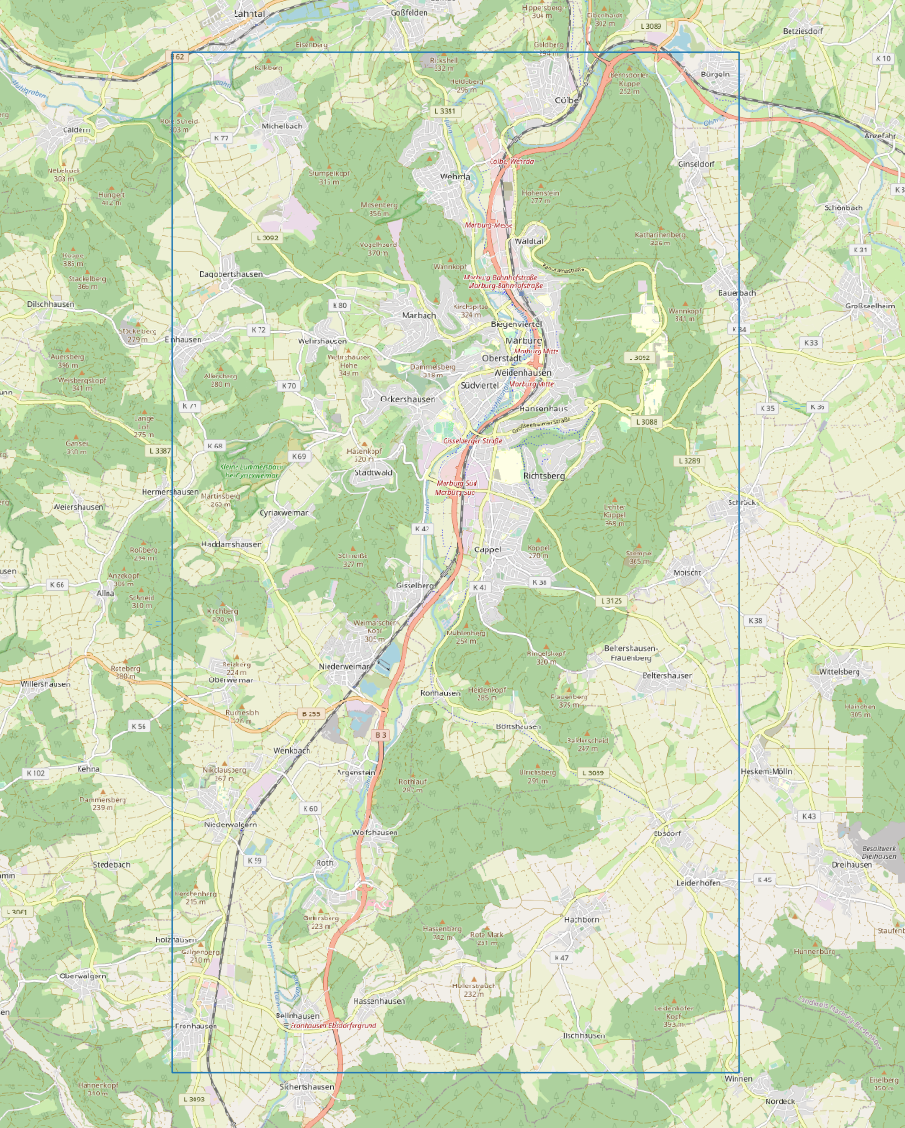
\includegraphics[width=1\linewidth,height=1\textheight]{C:/Users/kelto/Documents/iSEGMound/analysis/thesis/figures/Figure_18} 

}

\caption{Location of the case study area of this Master's thesis in county Marburg-Biedenkopf/Hesse, Germany. Scale 1:100 000}\label{fig:Figure18}
\end{figure}

The case study area was archaeologically investigated between 1983 and 1989 within the framework of a research project called ``Urnenfelderzeitliche Forschungen im Marburger Raum'' whose results were published in 1994 (Dobiat \emph{et al.} (1994)). This area constitutes the northernmost distribution of the South-German Urnfield Culture. Earlier studies led by the University of Marburg from the 1930's outlined the Marburg Group (mainly coined by Müller-Karpe (1949)) which based on the investigation between 1983 and 1989 can be broken down into multiple burial mound groups which extend over multiple hundreds of meters. Dobiat \emph{et al.} (1994), 9 postulated that originally more than 250 burial mounds must have existed which formed groups of up to a dozen mounds and are mainly situated along ridges looking over the Amöneburg Basin. East of Marburg, North to South sprawl the three burial mound groups Botanischer Garten, Lichter Küppel and Stempel (Figure 19). According to the estimation of Dobiat et al.~1994, 31, the burial mound group of Botanischer Garten should have consisted of about at least 40 burial mounds while the burial groups at Lichter Küppel and Stempel of around 30 burial mounds each.

\begin{figure}

{\centering 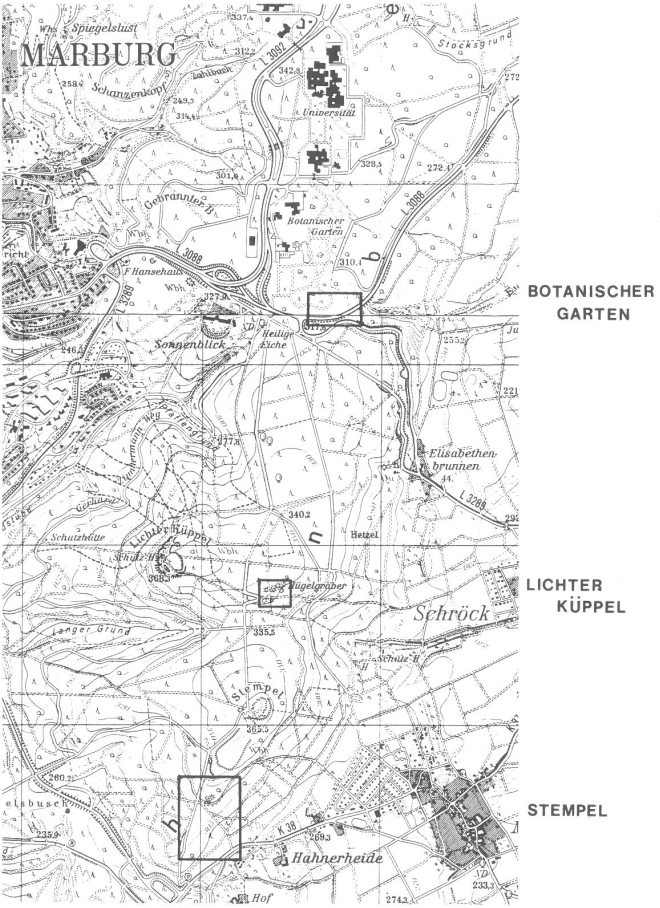
\includegraphics[width=0.75\linewidth,height=0.75\textheight]{C:/Users/kelto/Documents/iSEGMound/analysis/thesis/figures/Figure_19} 

}

\caption{The burial mound groups ‘Botanischer Garten’, ‘Lichter Küppel’ and ‘Stempel’. Dobiat et al. 1994, Supplement 1.}\label{fig:Figure19}
\end{figure}

The extent of the case study area of this thesis was chosen intentionally based on the discussed area in Dobiat \emph{et al.} (1994). After the 0.5 m DTM was calculated for the whole 180 km2 of the 20009/2010 LAZ files (see the workflow of the LiDAR data processing in 4.2), the attempt was made to identify all burial mounds in the Hillshade of the LiDAR derived 0.5 DTM by visual inspection in QGIS, based on the mapped burial mounds in Dobiat \emph{et al.} (1994) (Map Supplement 1 \& 2), also as a preparation to identify the Training Area and the Areas of Interests. Furthermore, apart from the already mentioned maps, Dobiat \emph{et al.} (1994) also provides lists of burial mounds: Liste 1 contains the burial mounds of the three main burial groups East of Marburg (`Botanischer Garten', `Lichter Küppel' and `Stempel') and Liste 2 contains the burial mounds in the broader Marburg area (West to Marburg, Area of Interest 1). The exact coordinates can be found in Dobiat \emph{et al.} (1994), 172-180.
During the visual comparison of the provided lists of mapped burial mounds and the hillshade of the case study area in QGIS the following differences have been documented:

\begin{longtable}[]{@{}rrrr@{}}
\caption{Comparison of the burial mound groups documented in Dobiat et al.~1994 and their visibility in the 2009/2010 LiDAR Hillshade. The sites which are marked with ? were not possible to identify in the Hillshade. NB: The burial mound groups 9 and 35 (the second mound) were only possible to identify using the Whitebox Multi-Scale Topographic Position Index derivative.}\tabularnewline
\toprule
Site ID & Dobiat et al. & DTM05 & AoI \\
\midrule
\endfirsthead
\toprule
Site ID & Dobiat et al. & DTM05 & AoI \\
\midrule
\endhead
1 & orig. 13 mounds & 10? visible & 4 \\
2 & 12 mounds & 5? visible & 4 \\
3 & orig. 5+2 mounds & 5 + 1 + 1 visible & 4 \\
4 & 5 mounds & 2 mounds visible? & 4 \\
5 & orig. 8 mounds & 9 visible & 4/training area \\
6 & 5 mounds & ? visible & 4 \\
7 & orig. 15 mounds & 9 visible & 4/training area \\
8 & 7 mounds & 4 visible & 4 \\
9 & 2 mounds & 1 in WB\_MTPI & 4/training area \\
10 & 8 mounds & 4 visible? & 4 \\
11 & 2 mounds & 2 visible & 4 \\
12 & orig. 20 mounds & \textasciitilde{} 7 visible & 4 \\
13 & 1 mound & 2 visible? & 4 \\
14 & 17-19 mounds & 18 visible & 4/training area \\
15 & 2+8 mounds & 2? visible & 4 \\
16 & orig. 4 mounds & ? & 3 \\
17 & 13 mounds & ? & 3 \\
18 & not existent & ? & 3 \\
19 & 5 mounds & ? & 3 \\
20 & 1 mound & 1? & 3 \\
21 & 7 mounds & 2? visible & 3 \\
22 & \textasciitilde{} 30 mounds & \textasciitilde13 visible & 3 \\
23 & 17 mounds & \textasciitilde11 visible & 3 \\
24 & 1 mound & 2? mounds & 3 \\
25 & ? mounds & ? & 3 \\
26 & 6 mounds & ? & 3 \\
27 & orig. 3 mounds & ? & 3 \\
28 & orig. 34 mounds & \textasciitilde17? & 3 \\
29 & min. 3 mounds & 3? & 3 \\
30 & 1 mound & ? & 2 \\
31 & ? mounds & ? & 2 \\
32 & 1 mound? & 1 visible & 2 \\
33 & 1 mound & ? & 2 \\
34 & 1 mound & 1 & 2 \\
35 & 2 mounds & 2 in WB\_MTPI & 4/training area \\
49 & 2x2 mounds & 2x2 mounds & 1 \\
51 & 1 + 2 mounds & 1 + 2 mounds & 1 \\
61 & 2 mounds & 2 mounds & 1 \\
\bottomrule
\end{longtable}

The concept of the workflow for the automated analysis of this data set was developed with keeping in mind that the burial mounds marked by `? ` will not be detected with a high probability, if they are not traceable in the Hillshade, even when using profile tools in QGIS. It was clear that using a 180 km2 area to develop workflows on is overpowering the computational capacity of a regular Laptop (Tuxedo with Ubuntu 18.04.5 LTS, i7, 15.4 GB RAM, no extra graphic card) and even Desktop PC (Windows 10, i7, 36 GB physical RAM \& 40.5 GB virtual RAM, NVIDIA GTX 1080), the data set was split up based on the investigation of the Hillshade of the case study area. First, all tiles were processed with 0.1 m resolution, but it was soon realized that any part of the workflow demanded exponentially more time per tile, than a tile with 0.5 m resolution, so the whole workflow is based on 0.5 m resolution.

The workflow developed was debugged in two instances: the workflow was first developed on the Training DTM, and then adapted to the Training Area. Then it was tested on five different Areas of Interests, which were chosen based on where the tumuli documented in Dobiat \emph{et al.} (1994) are located.
As Training DTM tile \emph{3dm\_32482\_5618\_1} was chosen (white box in Figure 20, left, with *`\_xyzirnc\_ground\_05'* suffix), because the burial mounds (Site IDs 5, 35 and 9, Figure 21) showed the biggest variability in size and were best preserved. Although it has to be said that even the Training DTM had surprises in store: Site ID 9 presented a quite a challenge to be identified - it was only possible to do so using the Multi-Scale Topographic Index implemented in Whitebox and accessed through R.
The Training Area (red box in Figure 20) consisting of five 1x1 tiles (\emph{3dm\_32482\_5616\_1\_he, 3dm\_32482\_5617\_1\_he, 3dm\_32482\_5618\_1\_he, 3dm\_32482\_5619\_1\_he, 3dm\_32483\_5616\_1\_he}, all with *`\_xyzirnc\_ground\_05'* suffix). Affiliated to these are the mound groups of Site ID 7 to the north, and Site ID 14, to the south (Figure 20, right).\\
The five Areas of Interest (AoI) are spatially disconnected were addressed clockwise:
Area of Interest 1: Site IDs 49, 51 \& 61 in List 2, Dobiat \emph{et al.} (1994), 177-178. Figure 21 \& 22.
Area of Interest 2: Site IDs 30 - 34 in List 1, Dobiat \emph{et al.} (1994), 175. See Figure 21 \& 22.
Area of Interest 3: `Botanischer Garten' and `Lichter Küppel', Site IDs 16 - 29 in List 1, Dobiat \emph{et al.} (1994), 174-175. Figure 21 \& 22.
Area of Interest 4: `Stempel', Site IDs 1 - 15 \& 35 in List 1, Dobiat \emph{et al.} (1994), 172-173 \& 175. Figure 21 \& 22.
Apart from the burial mounds mapped and discussed in Dobiat \emph{et al.} (1994), a few other burial mounds discernible in the Hillshade of the case study area were also included in the test dataset, that is AoI 5.
Area of Interest 5: 4 tiles west to Gisselberg, displaying 8(?) merovingian burial mounds in the west corner, but also other mound-like structures can be determined, actually throughout the whole case study area.

\begin{figure}
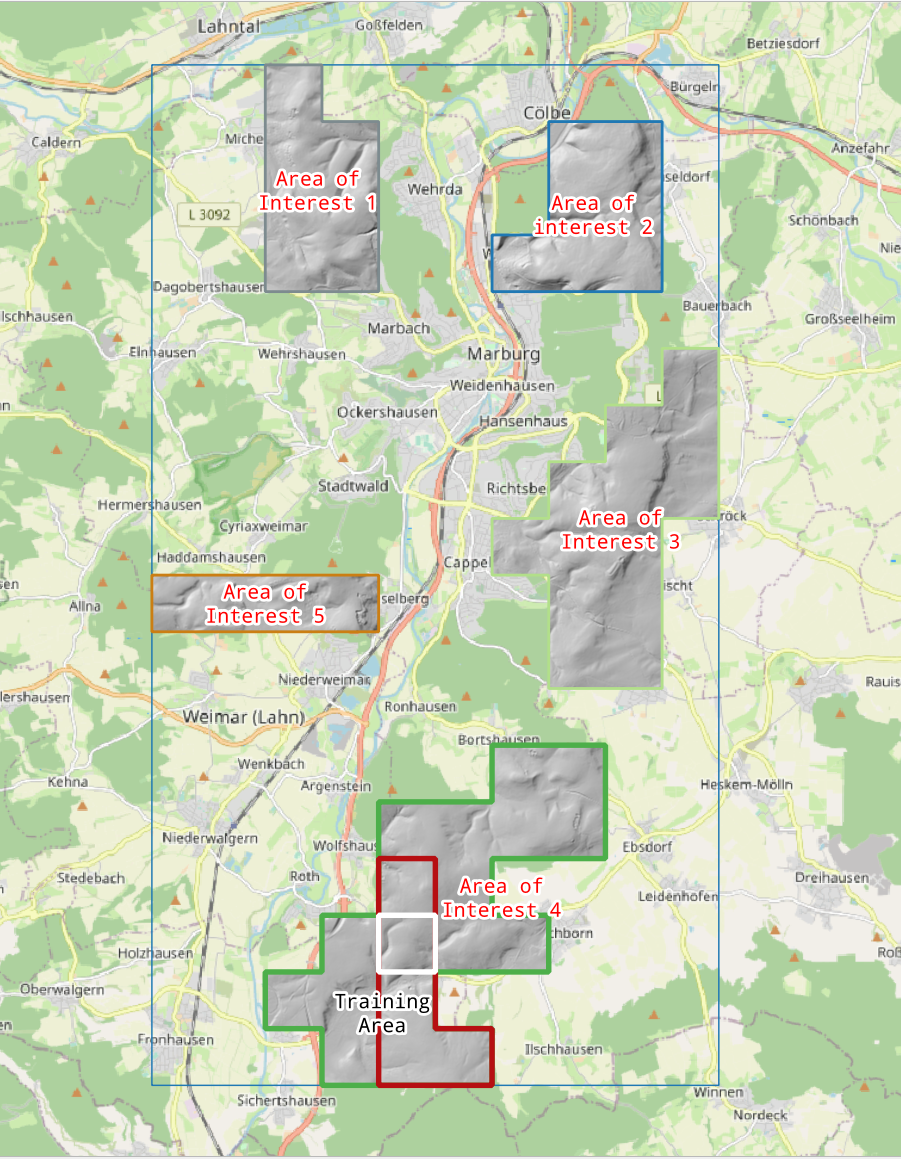
\includegraphics[width=0.5\linewidth,height=0.5\textheight]{C:/Users/kelto/Documents/iSEGMound/analysis/thesis/figures/Figure_20_1} 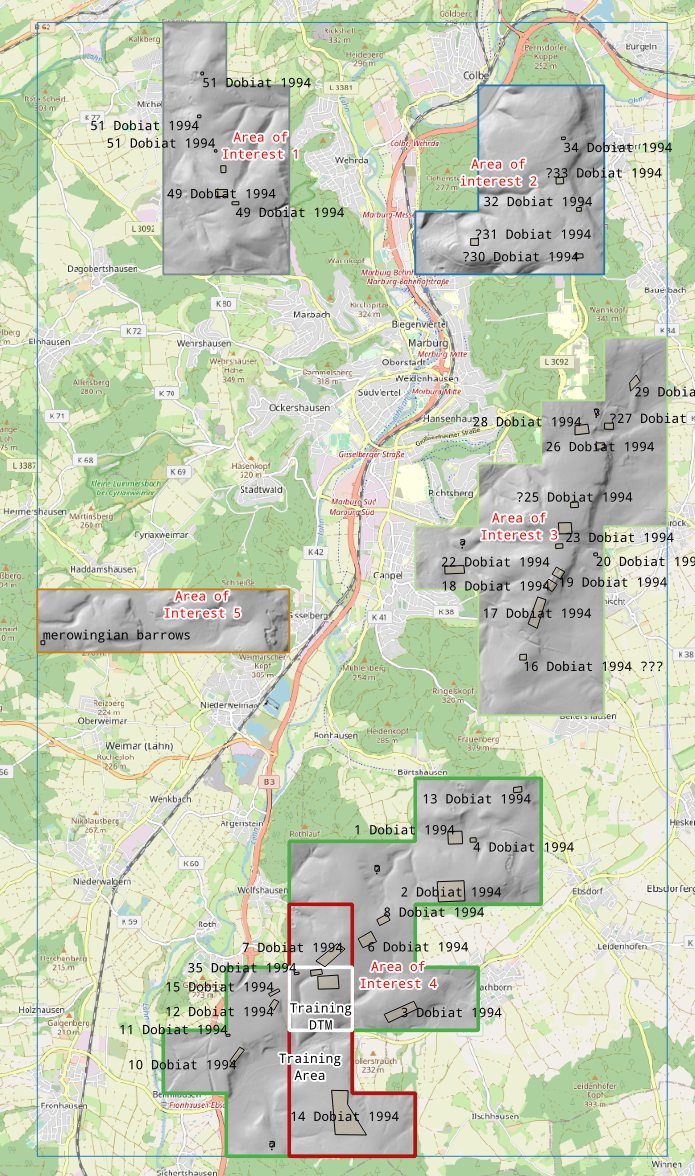
\includegraphics[width=0.5\linewidth,height=0.5\textheight]{C:/Users/kelto/Documents/iSEGMound/analysis/thesis/figures/Figure_20_2} \caption{Left:  Map and spatial relation of the Training DTM (white), the Training Area (red) and the five Areas of Interests (Area of Interest 1 = grey, Area of Interest 2 = blue, Area of Interest 3 = light green, Area of Interest 4 = grass green, Area of Interest 5 = orange). Right:The Training DTM, Training Area and the Area of Interests with the mapped burial mound sites in Dobiat et al. 1994. Scale 1:100 000}\label{fig:Figure20}
\end{figure}

To understand the nature and the morphological characteristics of the burial mounds in this area and also to understand if any change has happened since the LiDAR survey in 2009/2010, the Site IDs 5 and 35 were inspected in the terrain. At that time Site ID 9 was not identified in the \textbf{\emph{Hillshade}}. It has to be noted that for the main part of the Master's thesis the QGIS plugin `VoGIS Profile Tool' was used and only in a late phase of the work was the `Profile Tool' QGIS plugin discovered and used, which displays minimal changes in the terrain a lot better than the previous tool.
On May 10th in the afternoon the author and two colleagues (Simon Seyfried, a fellow student and Bjön Schmidt, now working in the Landesamt für Denkmalpflege in Wiesbaden) surveyed the area of the \textbf{Training DTM}. To identify the mounds, a polygon layer created in QGIS containing all identified mounds in the \textbf{Training DTM (Site IDs 5 and 35)} based on the visual inspection of the 0.5 m \textbf{\emph{Hillshade}} was exported to OruxMaps on an Android mobile phone to use as orientation and localisation.

\begin{figure}

{\centering 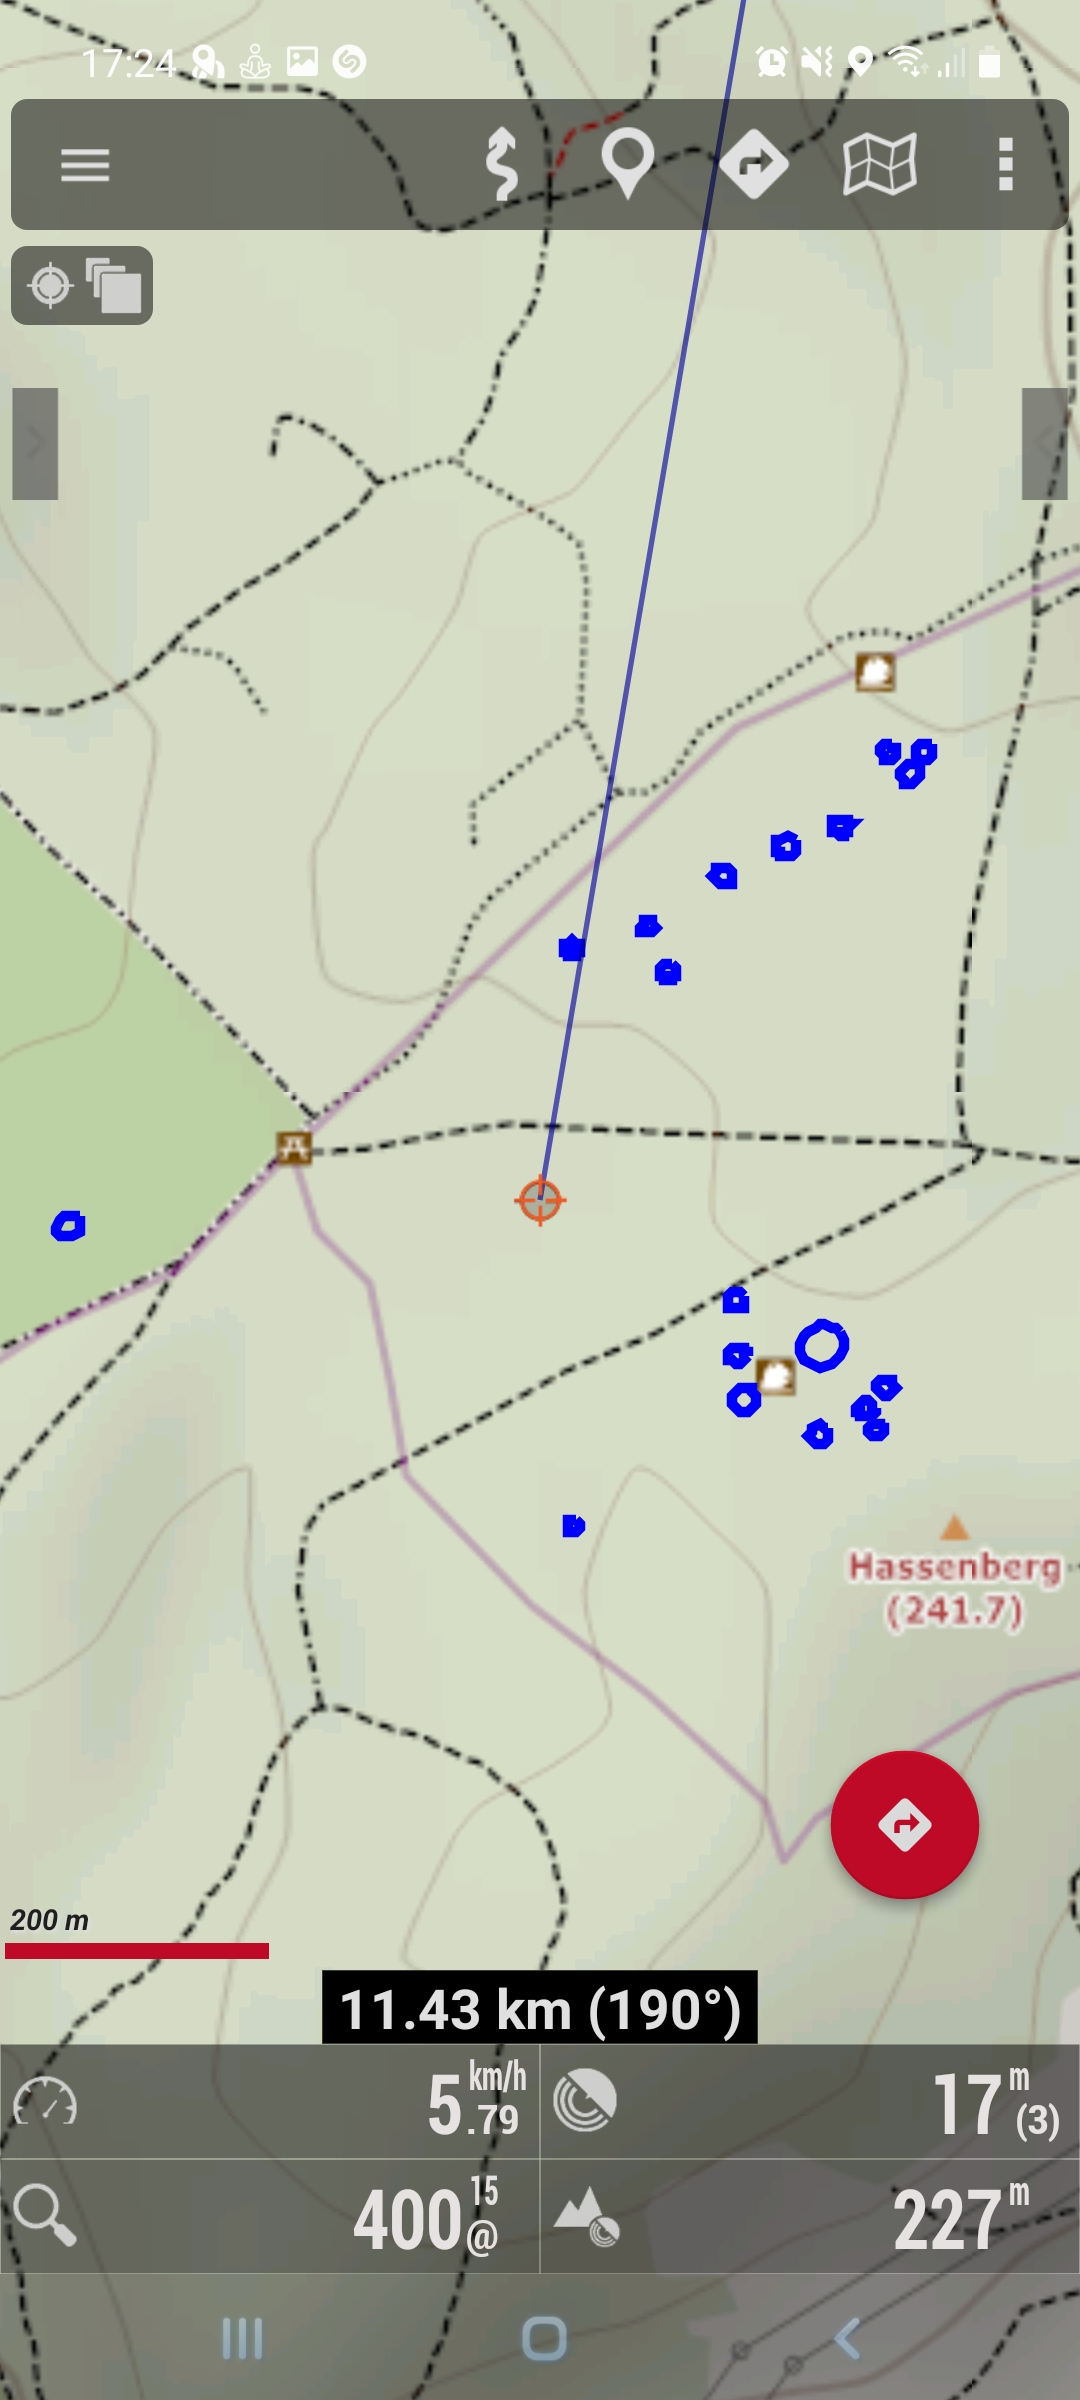
\includegraphics[width=0.4\linewidth,height=0.4\textheight]{C:/Users/kelto/Documents/iSEGMound/analysis/thesis/figures/Figure_21} 

}

\caption{Screenshot of Oruxmaps with the burial mounds with Site IDs 35 (to the West in the field), 5 (to the East in the forest), 7 (to the North, not investigated in the field). Only Site IDs 5 and 35 were investigated which can be found in the area of Training DTM.}\label{fig:Figure21}
\end{figure}

The first burial mounds to survey were \textbf{Site ID 35}. It was postulated from Dobiat \emph{et al.} (1994), that there might be two mounds present (Table 1). Figure 22 implies that it is only from the texture of the terrain that it is possible to guess any height difference between the two mounds. This is verified by the profile. It is clearly visible that \textbf{Site ID 35-1} is at most preserved up to around 38 cm in height. One of the surveyors is depicted in Figure 23 as a scale. \textbf{Site ID 35-2} is on a slope, already probably ploughed away, and/or the separating line (the 25 cm protuberance) in the field also destroyed a part of the second mound (Figure 22).

\begin{figure}
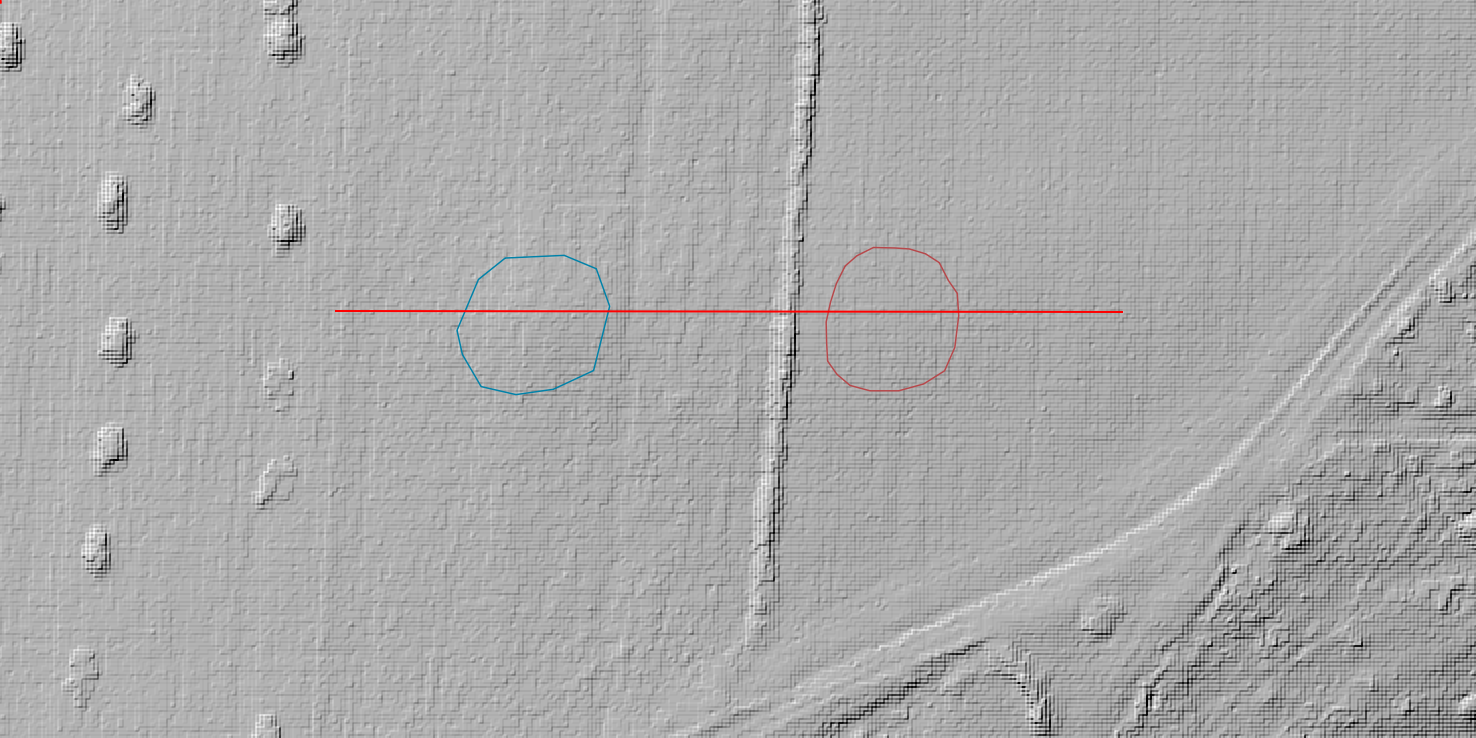
\includegraphics[width=0.5\linewidth,height=0.5\textheight]{C:/Users/kelto/Documents/iSEGMound/analysis/thesis/figures/Figure_22_1} 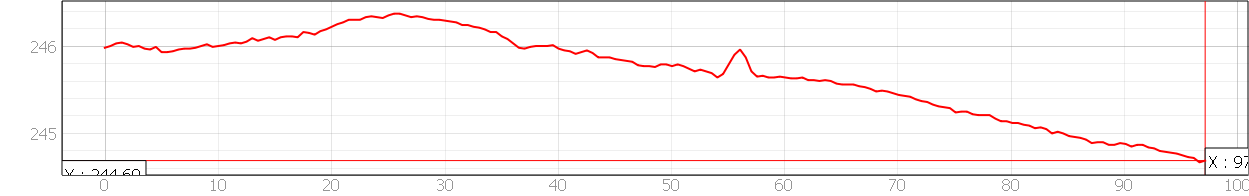
\includegraphics[width=0.5\linewidth,height=0.5\textheight]{C:/Users/kelto/Documents/iSEGMound/analysis/thesis/figures/Figure_22_2} \caption{Left: Location of burial mound group Site ID 35-1 and 2 in the Training DTM. Right: Profile of burial mound group, Site ID 35. Scale 1:700}\label{fig:Figure22}
\end{figure}
\begin{figure}

{\centering 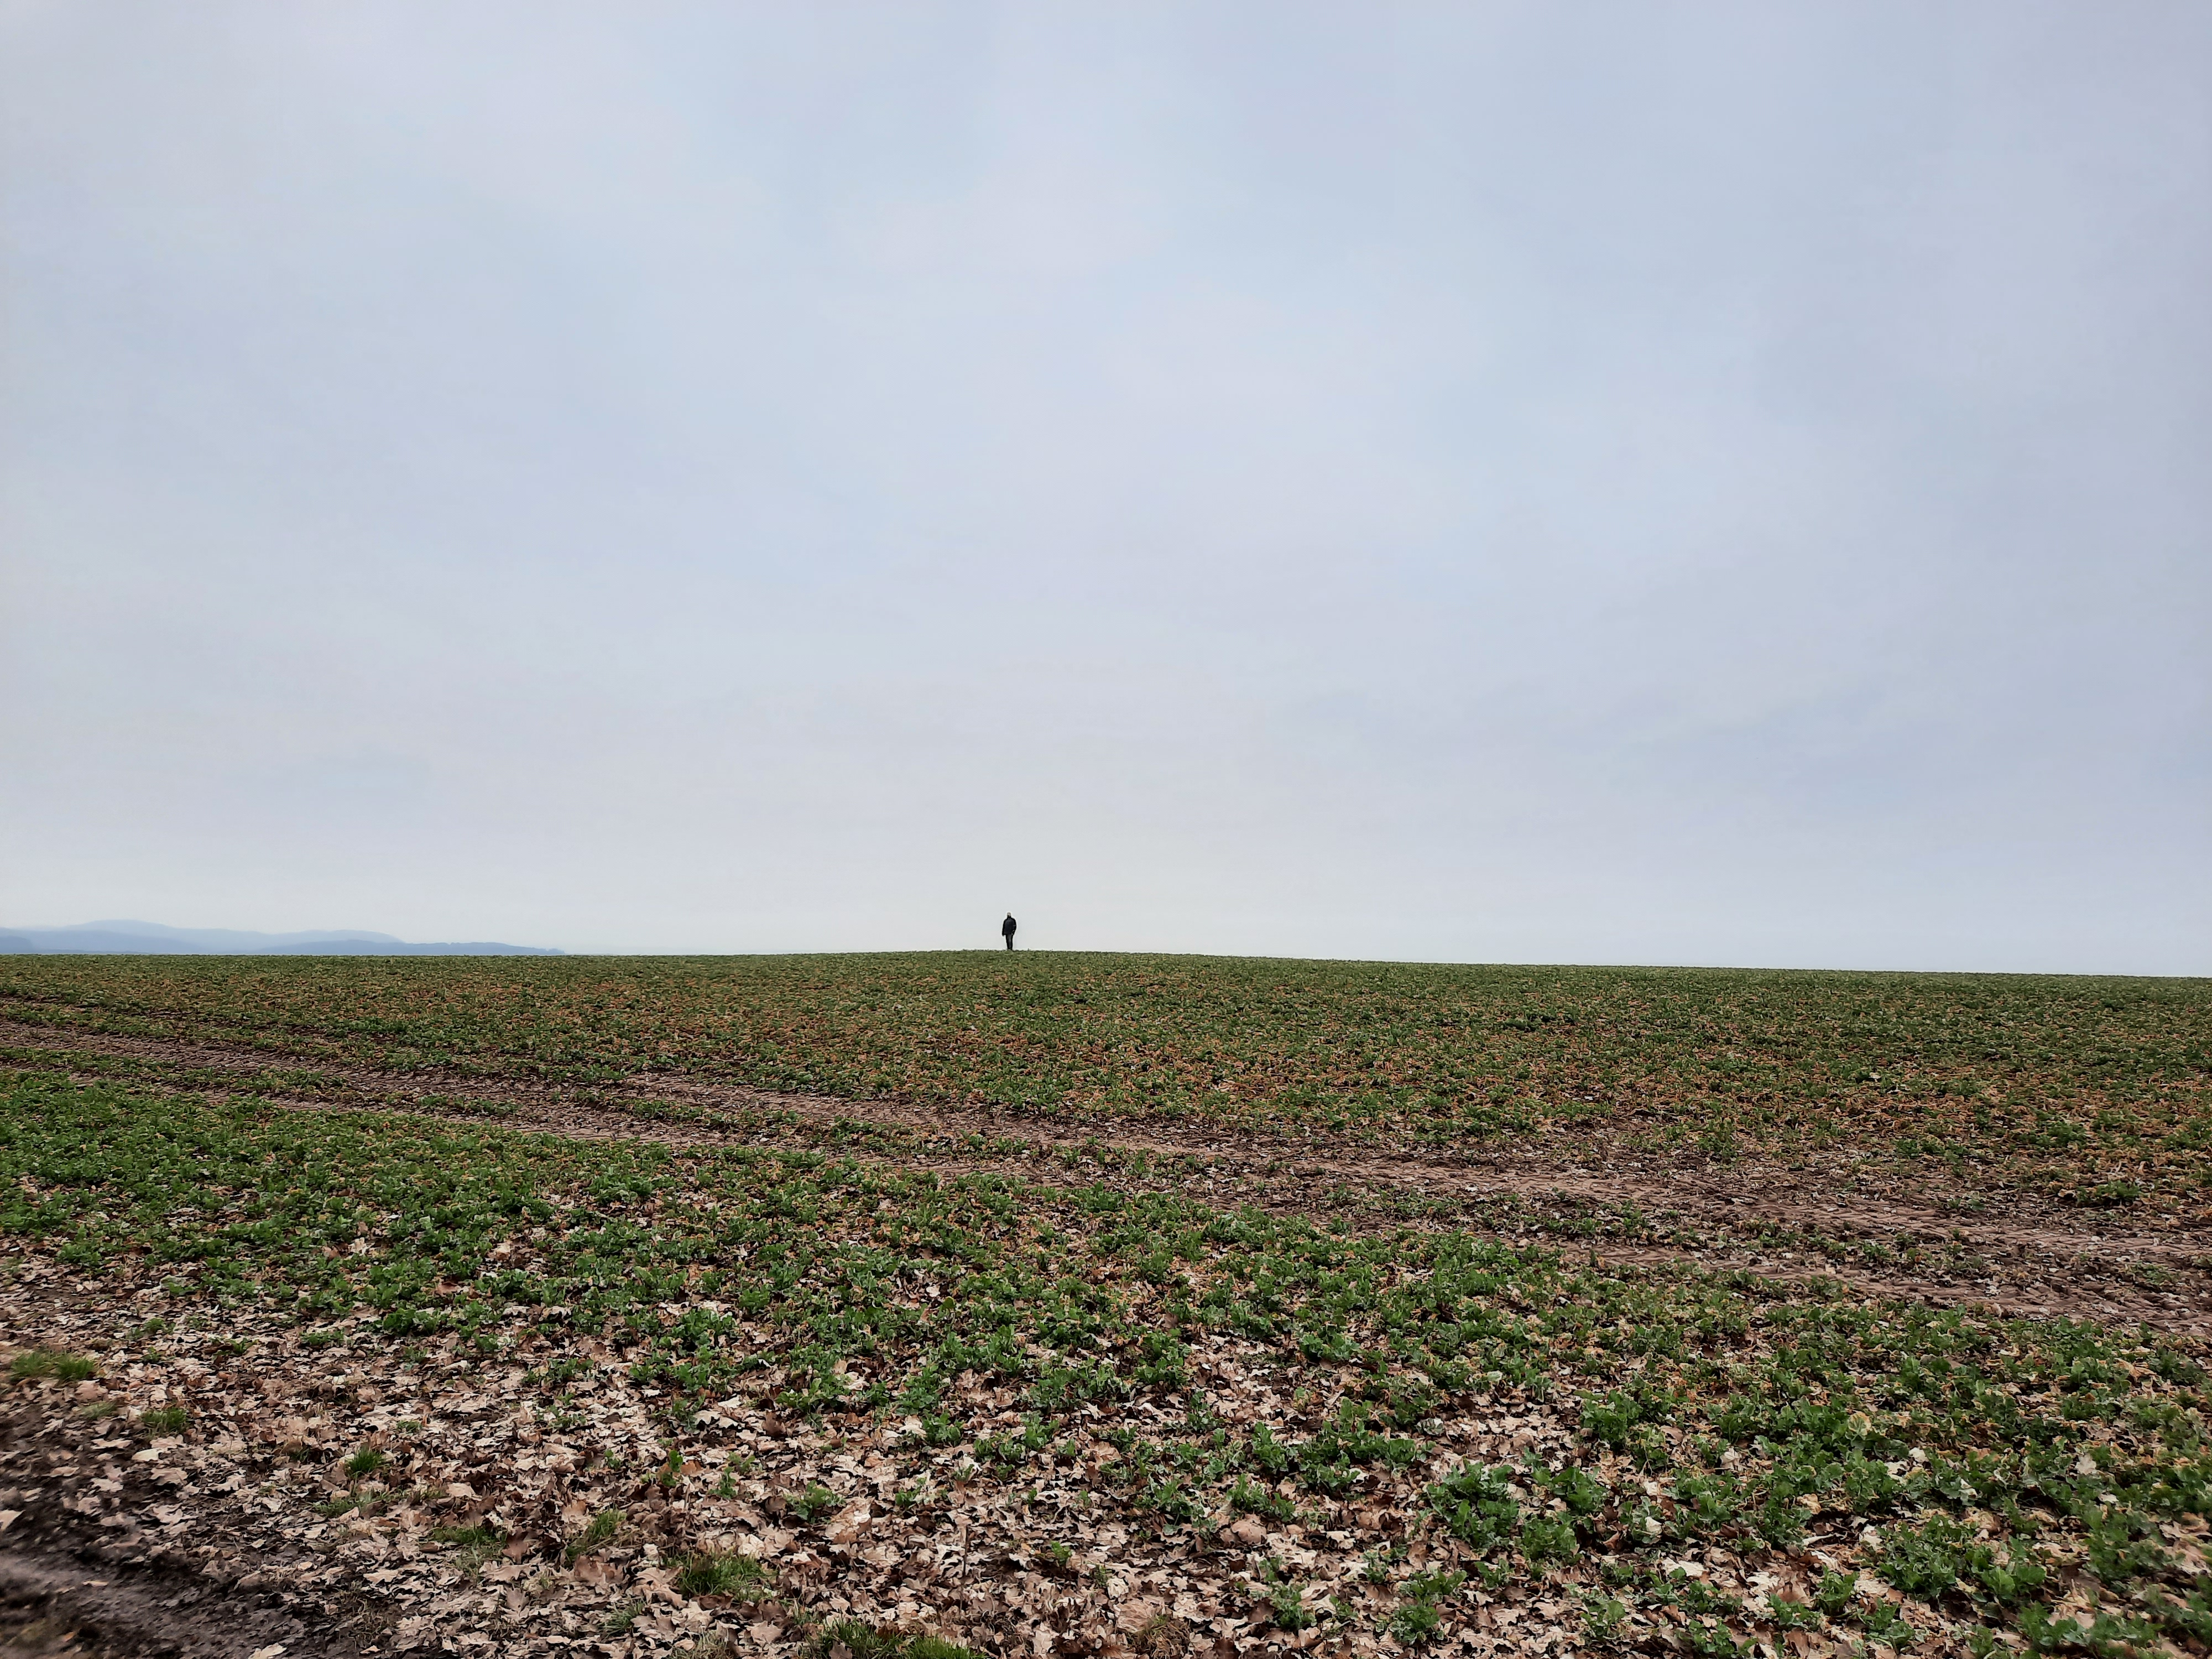
\includegraphics[width=0.7\linewidth,height=0.7\textheight]{C:/Users/kelto/Documents/iSEGMound/analysis/thesis/figures/Figure_23} 

}

\caption{Björn as scale on top of burial mound Site ID 35-1. The descending terrain can be only guessed.}\label{fig:Figure23}
\end{figure}

This was detected only when a \textbf{\emph{Multi-Scale Topographic Position Index}} using the \texttt{whitebox} package was calculated (Figure 24). This derivative was not taken into account when building the workflow, because the \texttt{whitebox\ R\ package} (which is the R interface for the \textbf{Whitebox GAT FOSS GIS software}) did not work when working with the Tuxedo laptop and Windows 10 Desktop PC. Since then the bug was fixed in the next update. The \textbf{\emph{Multi-Scale Topographic Position Index}} will be discussed more in depth later on.
Generally it can be said that burial mounds which are situated in agricultural fields (that is in an intensively used area) are more likely to be detected by multispectral drone imagery and the calculation of vegetation indices than by LiDAR derived DTMs. Thus it was a pleasant surprise to see the traces of the two burial mounds of Site ID 35 (at least presumably also the second - and maybe a third?) in the \textbf{Train DTM /Train Area/Area of Interest 4} using the \textbf{\emph{Multi-Scale Topographic Position Index}}. The question is if burial mound \textbf{Site ID 35-2} has eroded so much in the last 20 years (since 1994) that it is not possible any more to clearly detect it and only to try to guess it's location. In Figure 24 the yellow areas delineate areas which are elevated in the micro-, meso- and macro scale, thus exaggerating the topography. On this basis also the area right to Site ID 35-2 might be arguable, but when we look at the extended profile, the section between 50 and 70 meters on the Y axis is most probable, but definitely eroded and disturbed by the field separator.

\begin{figure}
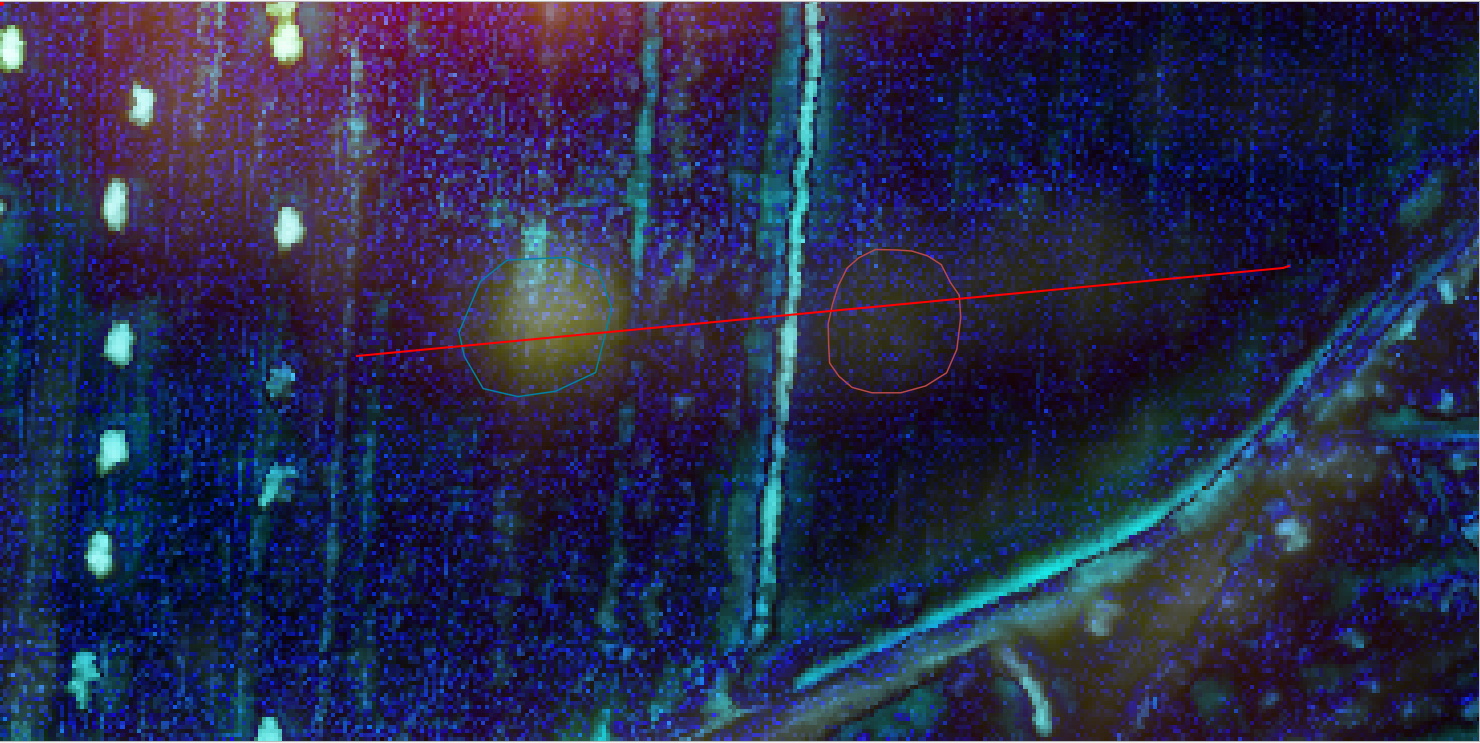
\includegraphics[width=0.5\linewidth,height=0.5\textheight]{C:/Users/kelto/Documents/iSEGMound/analysis/thesis/figures/Figure_24_1} 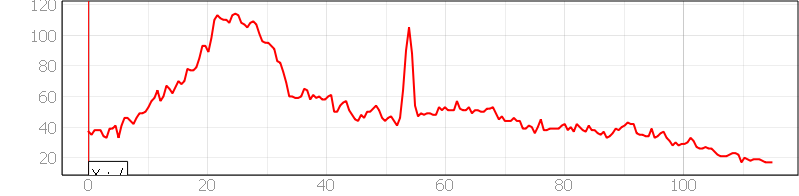
\includegraphics[width=0.5\linewidth,height=0.5\textheight]{C:/Users/kelto/Documents/iSEGMound/analysis/thesis/figures/Figure_24_2} \caption{Left: The Multi-Scale Topographic Position Index calculated using the whitebox package in R, with the burial mound groups Site ID 35-1 and 35-2, possibly 35-3?. Right: Extended and intentionally positioned profile of burial mound group Site ID 35. Note the scale is different being an MTPI. Scale 1:700}\label{fig:Figure24}
\end{figure}

The burial mounds of \textbf{Site ID 5(-1 to -9)} are much more clearer to identify, as is visible from Figure 25. To make it easier to spot Site ID 5-9, the burial mound polygons are projected on the \textbf{\emph{Hillshade}} with 25\% transparency. \textbf{Site ID 5} is the complete opposite of \textbf{Site ID 35} - the mounds are extremely well discernable in the 0.5 m \textbf{\emph{Hillshade}}, only to realize that when checking their profile, that their peak is mainly less than half a meter. Only Site ID 5-1 and 5 are outliers according to their height.

\begin{figure}
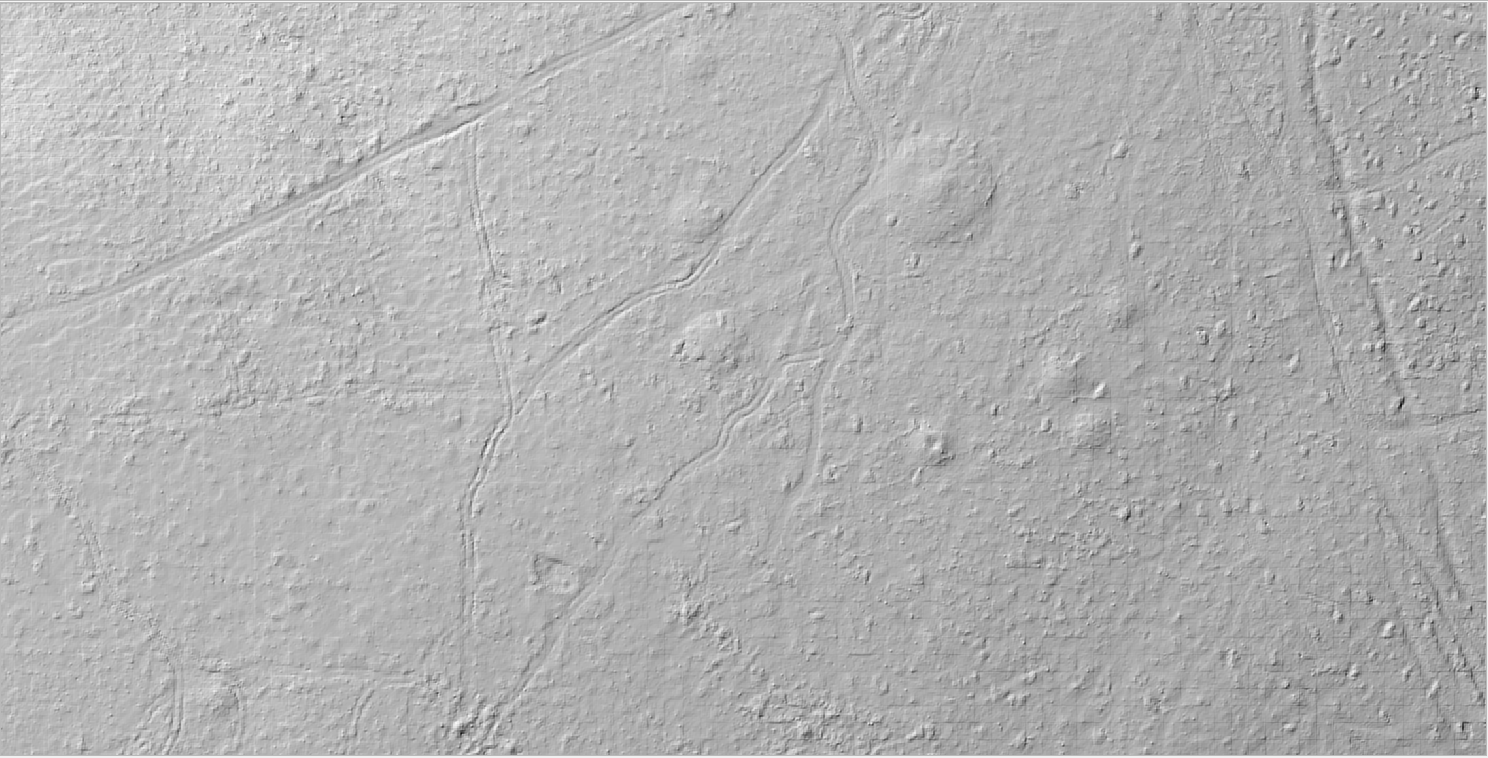
\includegraphics[width=0.5\linewidth,height=0.5\textheight]{C:/Users/kelto/Documents/iSEGMound/analysis/thesis/figures/Figure_25_1} 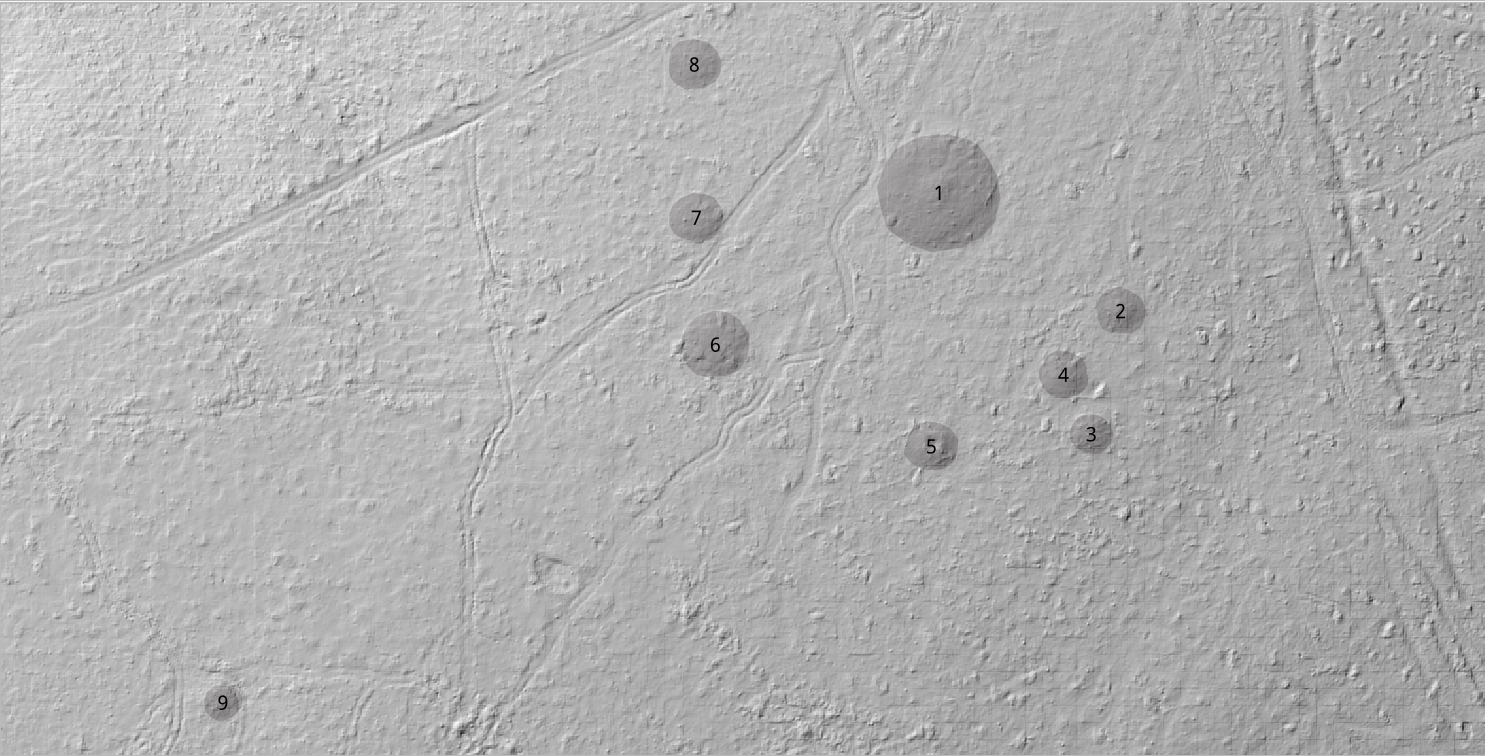
\includegraphics[width=0.5\linewidth,height=0.5\textheight]{C:/Users/kelto/Documents/iSEGMound/analysis/thesis/figures/Figure_25_2} \caption{Left: Hillshade of Site ID 5. Right: Hillshade of Site ID 5 overlayed by transparent mound polygons. Scale 1:1500}\label{fig:Figure25}
\end{figure}

The approximative height measurements of the burial mounds are as follows:
Site ID 5-1 \textasciitilde{} 120 cm
\newline
Site ID 5-2 \textasciitilde{} 40 cm
\newline
Site ID 5-3 \textasciitilde{} 38 cm
\newline
Site ID 5-4 \textasciitilde{} 42 cm
\newline
Site ID 5-5 \textasciitilde{} 50 cm
\newline
Site ID 5-6 \textasciitilde{} 60 cm
\newline
Site ID 5-7 \textasciitilde{} 50 cm
\newline
Site ID 5-8 \textasciitilde{} 45 cm
\newline
Site ID 5-9 \textasciitilde{} 40 cm

Below the profiles and the location of the profiles of the individual burial mounds are depicted for clarification (Figure 26).

\begin{figure}
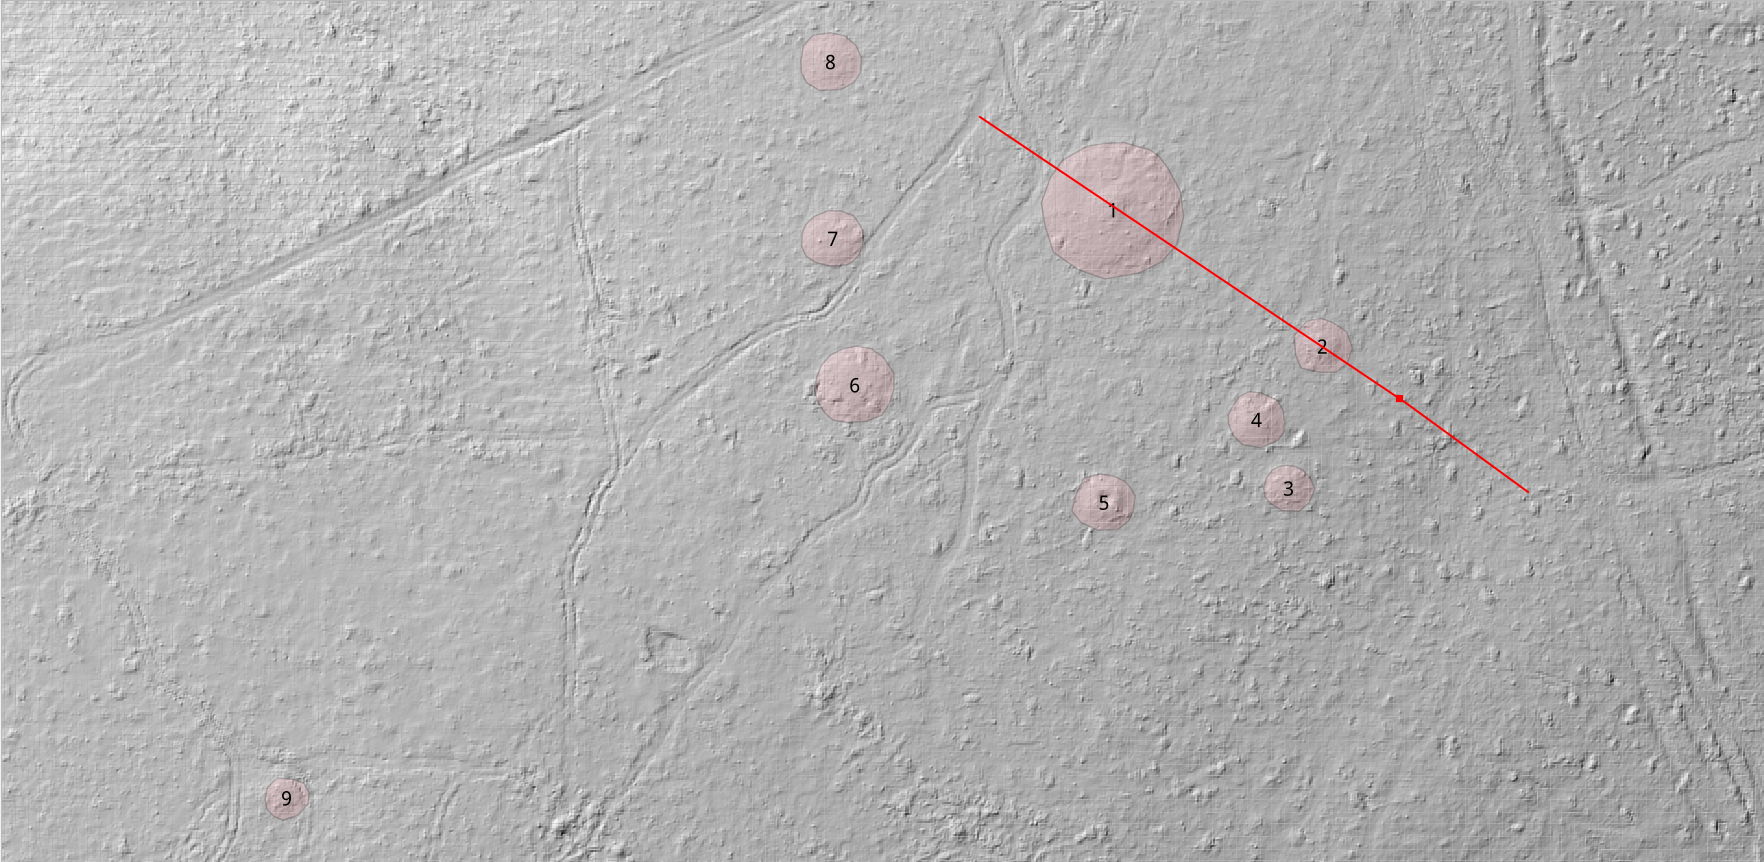
\includegraphics[width=0.5\linewidth,height=0.5\textheight]{C:/Users/kelto/Documents/iSEGMound/analysis/thesis/figures/Figure_26_1} 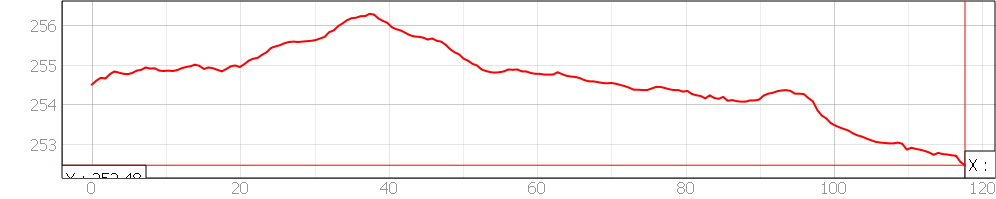
\includegraphics[width=0.5\linewidth,height=0.5\textheight]{C:/Users/kelto/Documents/iSEGMound/analysis/thesis/figures/Figure_26_2} 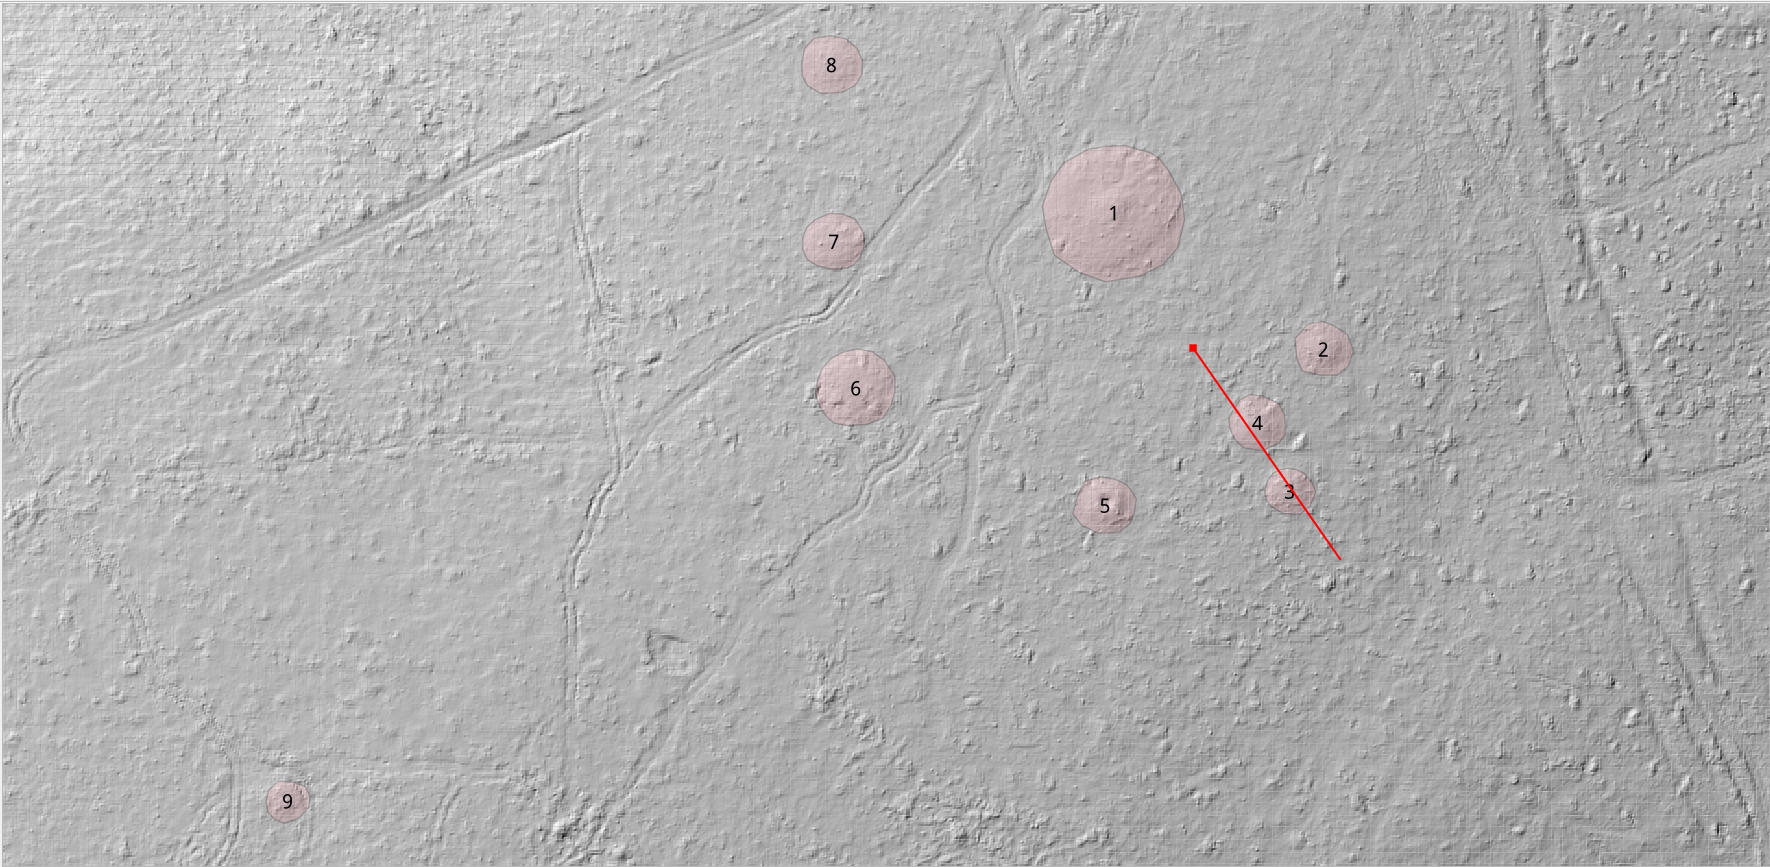
\includegraphics[width=0.5\linewidth,height=0.5\textheight]{C:/Users/kelto/Documents/iSEGMound/analysis/thesis/figures/Figure_26_3} 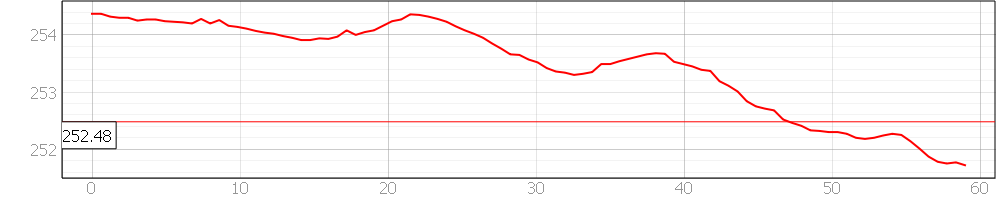
\includegraphics[width=0.5\linewidth,height=0.5\textheight]{C:/Users/kelto/Documents/iSEGMound/analysis/thesis/figures/Figure_26_4} 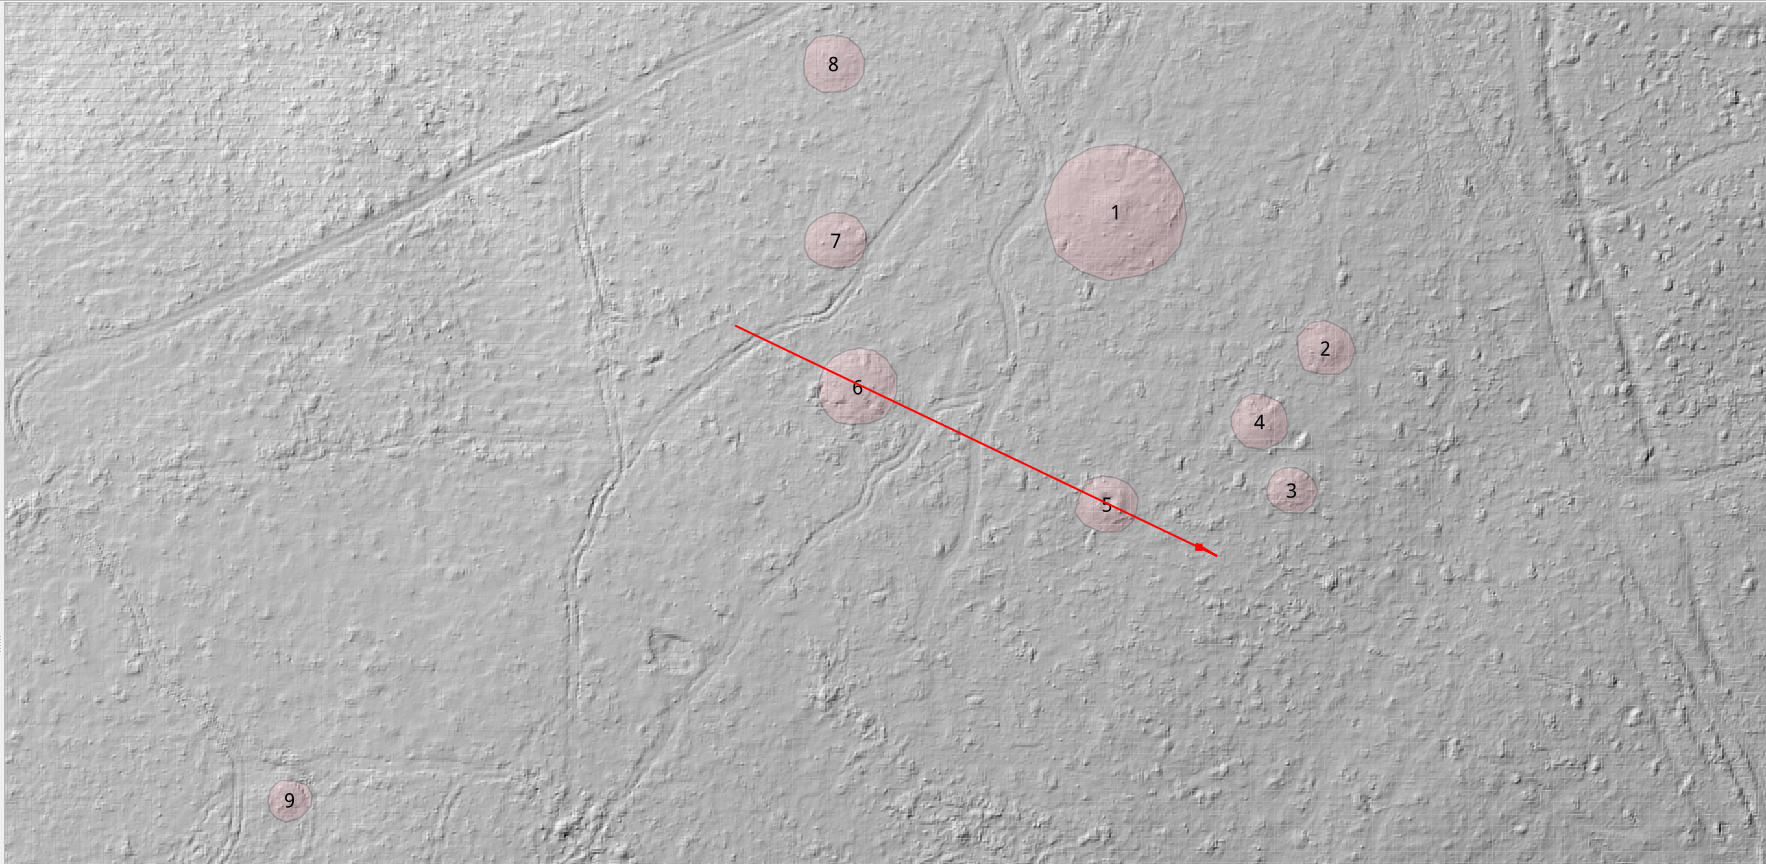
\includegraphics[width=0.5\linewidth,height=0.5\textheight]{C:/Users/kelto/Documents/iSEGMound/analysis/thesis/figures/Figure_26_5} 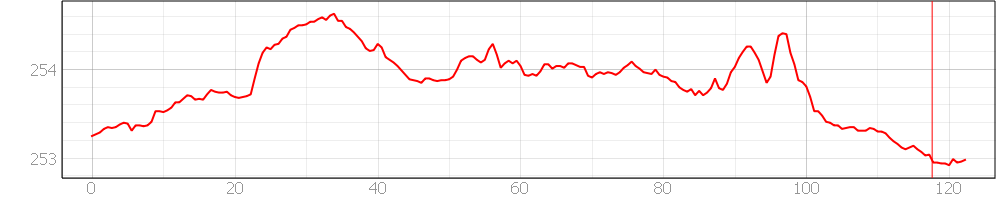
\includegraphics[width=0.5\linewidth,height=0.5\textheight]{C:/Users/kelto/Documents/iSEGMound/analysis/thesis/figures/Figure_26_6} 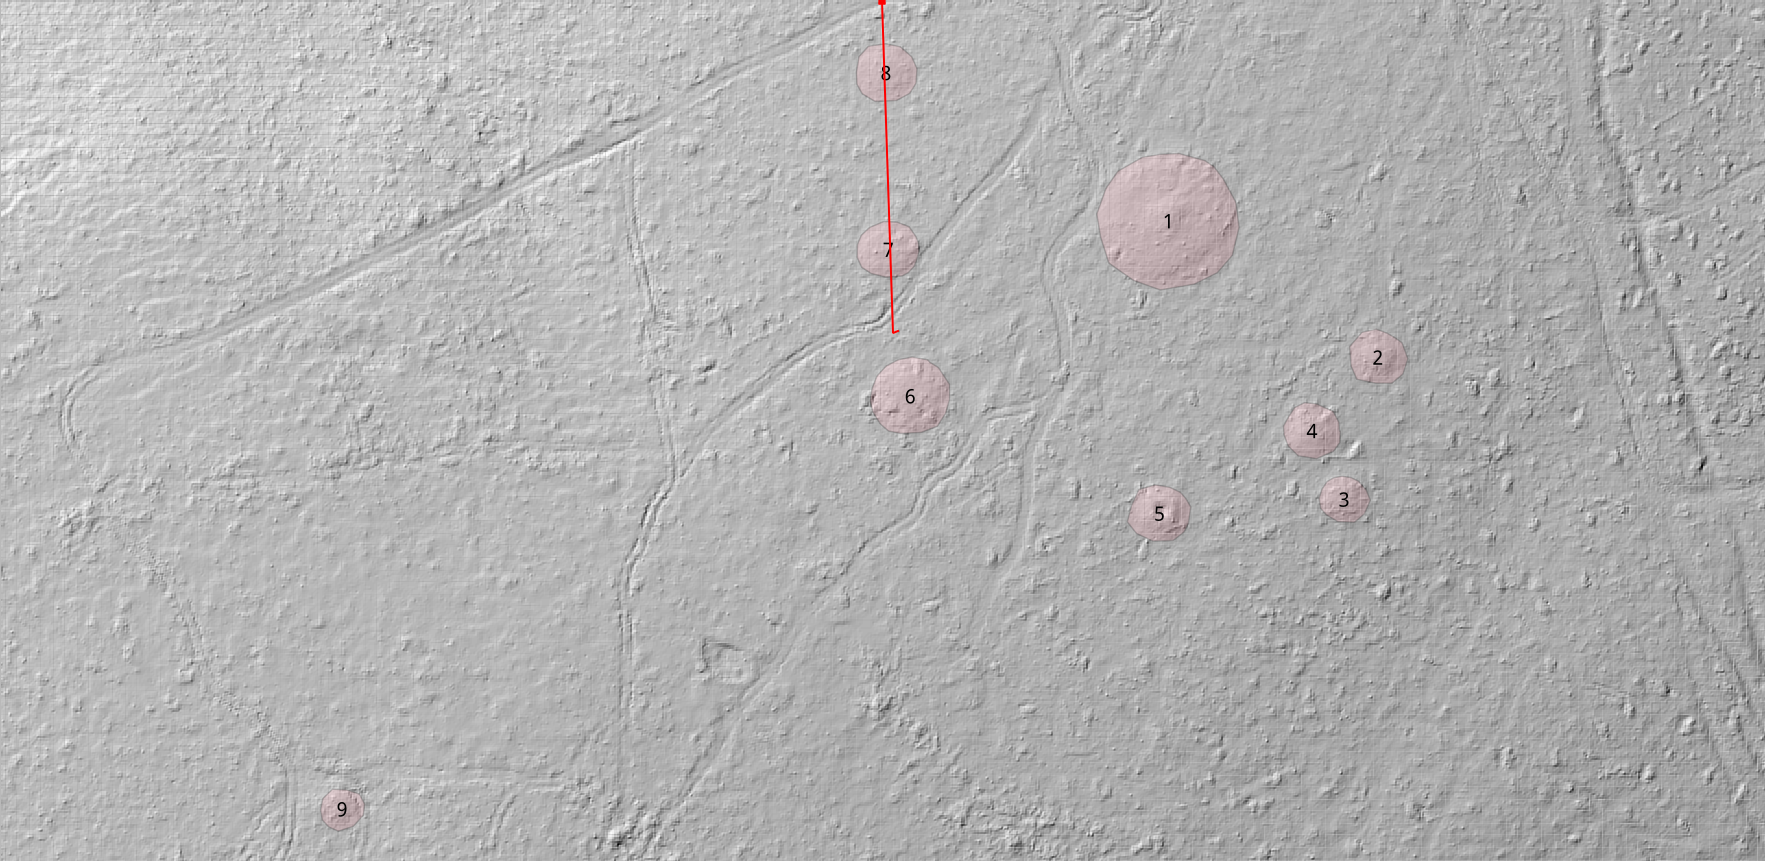
\includegraphics[width=0.5\linewidth,height=0.5\textheight]{C:/Users/kelto/Documents/iSEGMound/analysis/thesis/figures/Figure_26_7} 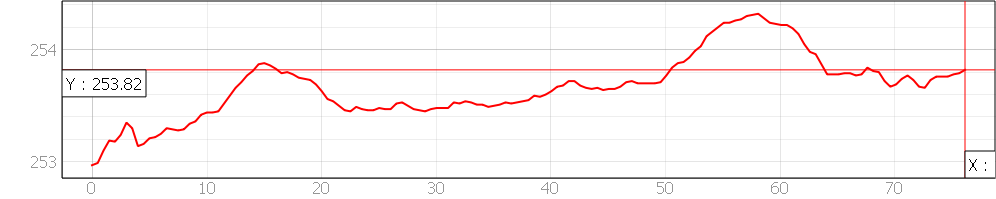
\includegraphics[width=0.5\linewidth,height=0.5\textheight]{C:/Users/kelto/Documents/iSEGMound/analysis/thesis/figures/Figure_26_8} 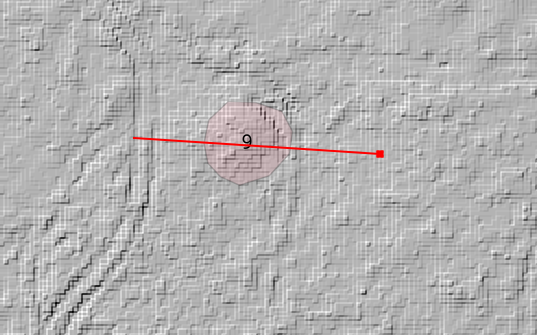
\includegraphics[width=0.5\linewidth,height=0.5\textheight]{C:/Users/kelto/Documents/iSEGMound/analysis/thesis/figures/Figure_26_9} 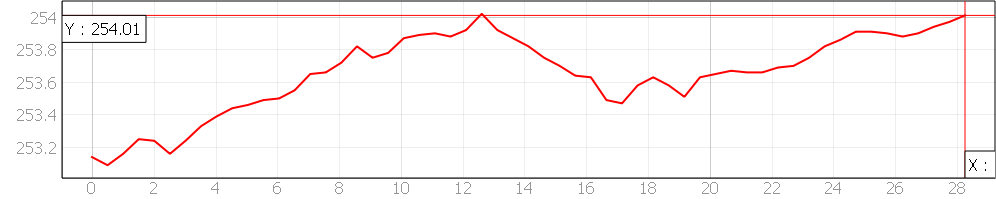
\includegraphics[width=0.5\linewidth,height=0.5\textheight]{C:/Users/kelto/Documents/iSEGMound/analysis/thesis/figures/Figure_26_10} \caption{Left row: Hillshade of Site ID 5-1 to 9. Right row: Profile of Site ID 5 5-1 to 9 overlayed by transparent mound polygons. Scale 1:1500}\label{fig:Figure26}
\end{figure}

To sum up it can be said that most of the burial mounds of Site ID 5 were easily identified in the terrain, apart from \textbf{Site ID 5-9}. In Figures 26-9 and 26-10 traces of big agricultural machines are visible which makes sense, given that there is a concrete road in the vicinity as seen in Figure 27. The situation discernable in the Hillshade has apparently worsened in the last 10 years. Figure 27 illustrates the local topography of \textbf{Site ID 5-9} (center illustrated with red stick) to demonstrate that if it weren't for Oruxmaps and the shapefile of the burial mounds, the field identification of the mound would've been completely missed. This also suggests that other less well preserved or barely visible sites in the LiDAR data from 2009/10 might also be more eroded or even completely diminished.
All this information has to be kept in mind when choosing automated analysis methods. Only because a certain method is working for burial mounds or mound-like archaeological objects in a certain region, it might not be true for other regions. Because topography in general, the micro-topography and especially geomorphology (and their way of erosion) play a very important role in how archaeological objects change with time and also how they are preserved in the present state when they are being investigated. In these cases a compromise has to be made to successfully detect barrows as will be demonstrated in the following sub-chapters.

\begin{figure}

{\centering \includegraphics[width=0.7\linewidth,height=0.7\textheight]{C:/Users/kelto/Documents/iSEGMound/analysis/thesis/figures/Figure_27} 

}

\caption{Documentation of burial mound group Site ID 5-9 in the field.}\label{fig:Figure27}
\end{figure}

\hypertarget{the-general-workflow-of-automated-analysis-methods}{%
\subsection{\texorpdfstring{\textbf{The General Workflow of Automated Analysis Methods}}{The General Workflow of Automated Analysis Methods}}\label{the-general-workflow-of-automated-analysis-methods}}

When undertaking automated analysis of remote sensing data, there are certain general steps to be followed - clearly outlining themselves in the surveyed studies and depending on what data type is at disposal. If DTM/DEM raster are available, Data Pre-Processing (step i) would be unnecessary. Also, some methods and workflows do not require data preparation (they directly use the DEM/DTMs) and start right away with Data Analysis (iii), which can be (as already detailed in Chapter 2) a combination of Geometric knowledge-based Analysis, GeOBIA and/or Machine Learning or single methods. In step iii the respective methods used in this thesis are investigated and discussed (iii-i and iii-ii). The last step (iv) is of course the verification of the results. A generalized workflow would look the following (see also Figure 28):

\begin{figure}

{\centering 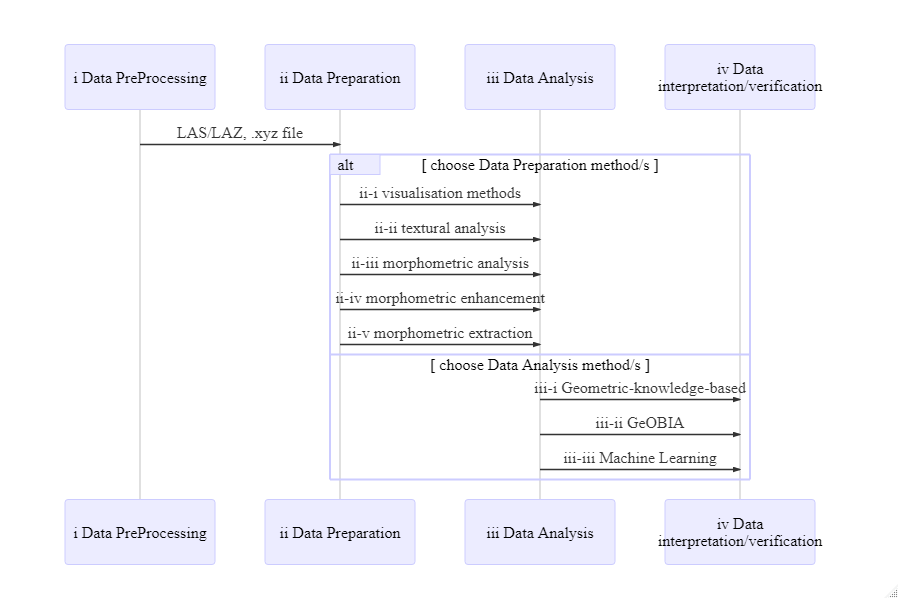
\includegraphics[width=1\linewidth,height=0.7\textheight]{C:/Users/kelto/Documents/iSEGMound/analysis/thesis/figures/Figure_28} 

}

\caption{Generalized workflow of automated analysis of archaeological remote sensing datasets.}\label{fig:Figure28}
\end{figure}

\hypertarget{data-pre-processing}{%
\subsection{\texorpdfstring{\textbf{Data Pre-Processing}}{Data Pre-Processing}}\label{data-pre-processing}}

The LiDAR dataset from 2009/2010 of the case study area is processed by the state-of-the art point-cloud oriented \texttt{lidR\ package} (Roussel \emph{et al.} (2020)) which makes it easy to manipulate and analyse LiDAR datasets and is FOSS. Multiple functions, algorithms, methods and workflows presented in peer-reviewed literature are implemented and thus \texttt{lidR} enables users to make specialized workflows and thus functions as a toolbox (Roussel \emph{et al.} (2020)).
It has to be mentioned, that according personal communication with the ``Hessisches Landesamt für Bodenmanagement und Geoinformation'' no metadata exists for the LiDAR data set from 2009/10, thus all inofrmation exisits it converyed in the .LAZ header and can be accessed using the `lidR package.

\hypertarget{dtm-generation-by-testing-different-algorithms}{%
\subsubsection{\texorpdfstring{\textbf{DTM Generation by Testing Different Algorithms}}{DTM Generation by Testing Different Algorithms}}\label{dtm-generation-by-testing-different-algorithms}}

As a first step it was tested which ground point re-/classification and spatial interpolation should be used to generate a DTM which can capture all geomorphological details in the terrain that can be used to detect burial mounds. The processing of LiDAR data is a basic but very important part of the workflow. Still, it is only a means to an end so it will be kept brief (but in the necessary length to provide ideas to others who want to process LiDAR data for archaeological use using the \texttt{lidR\ package}) so that the focus can be oriented towards the detection of burial mounds.

\begin{figure}

{\centering 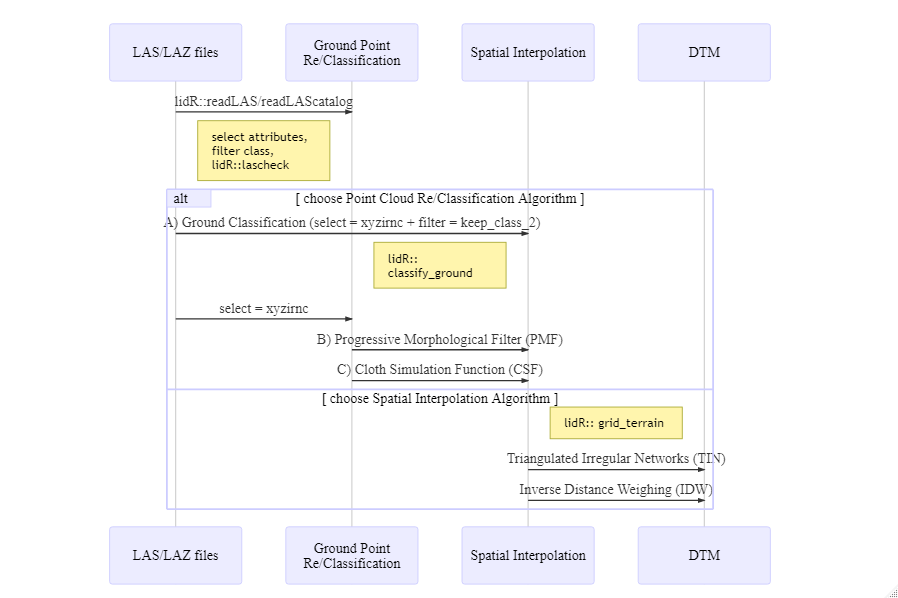
\includegraphics[width=1\linewidth,height=0.7\textheight]{C:/Users/kelto/Documents/iSEGMound/analysis/thesis/figures/Figure_29} 

}

\caption{Workflow of the LiDAR data processing.}\label{fig:Figure29}
\end{figure}

For the comparison of the algorithms one random LAS tile was processed to understand the needed steps to generate at a DTM with as few artifacts and noise as possible, but detailed enough to still contain the information important for the Objects of Interest. A random tile was chosen, because when getting a point cloud data set we do not know yet where exactly our Objects of Interests are.
The steps undertaken and tested are depicted and summarized in Figure 29. The complete code for this subchapter can be found in script \textbf{2\_LiDAR\_data\_processing\_tile\_1.R}. Here only relevant chunks are displayed.

\textbf{4.3.1.0 Get to know the point cloud}\\
\newline
LAS files store x,y,z for each point and many other information/attributes and this can claim a lot of memory from the PC.

\begin{Shaded}
\begin{Highlighting}[]
\FunctionTok{names}\NormalTok{(LIDR\_200910\_1}\SpecialCharTok{@}\NormalTok{data)}
\end{Highlighting}
\end{Shaded}

The `select' argument enables you to choose between attributes/columns. The queries are:
\newline
\texttt{t\ -\ gpstime,\ a\ -\ scan\ angle,\ i\ -\ intensity,\ n\ -\ number\ of\ returns,\ r\ -\ return\ number,\ c\ -\ classification,\ s\ -\ synthetic\ flag,\ k\ -\ keypoint\ flag,\ w\ -\ withheld\ flag,\ o\ -\ overlap\ flag\ (format\ 6+),\ u\ -\ user\ data,\ p\ -\ point\ source\ \#ID,\ e\ -\ edge\ of\ flight\ line\ flag,\ d\ -\ direction\ of\ scan\ flag}

The `filter' argument enables you to choose between the rows/points with specific attributes. The filter options can be accessed by: \texttt{read.las(filter\ =\ "-help")}

\emph{Note: when using the select and filter arguments with readLAS, it allows you to filter while reading the LAS file thus saving memory and computation time - it is the same as reading the LAS file and then filtering the point cloud but saving memory and computation time.}

On this ground it was decided that the following arguments are needed: \emph{x,y,z, return number and number of returns, intensity, classification:}

\begin{Shaded}
\begin{Highlighting}[]
\NormalTok{LIDR\_200910\_1\_xyzirnc }\OtherTok{\textless{}{-}}\NormalTok{ lidR}\SpecialCharTok{::}\FunctionTok{readLAS}\NormalTok{(lsLIDAR\_2009\_10[}\DecValTok{1}\NormalTok{], }\AttributeTok{select =} \StringTok{"xyzirnc"}\NormalTok{)}
\end{Highlighting}
\end{Shaded}

\textbf{4.3.1.1 Ground point re/classification}
\newline
The next step involves the re/classification of the ground points of the LiDAR point cloud. This serves as a foundation for the DTM generation.
LAS point clouds already have a classification (as noted above) according to the ASPRS Society, which has explicit LAS specifications \href{https://www.asprs.org/wp-content/uploads/2010/12/LAS_1_4_r13.pdf}{LAS specifications}. Class 2 corresponds to the ground points.
Two ground (re)classification algorithms are implemented in \texttt{lidR}: the Progressive Morphological Filter (PMF) and the Cloth Simulation Function (CSF). Both reclassify the classified ground point as unclassified before (re)classifying them.
The aim of this chapter is to understand if the existing ground classification can be improved by reclassifying the point cloud and if the amount of testing is worth the time. Thus the PMF and CSF algorithms and the existing ground classification are compared if they can return an even more accurate model of the ground surface.

\textbf{A) Ground Classification}
\newline
\textbf{\emph{i LIDR\_200910\_1\_ground}}

\begin{Shaded}
\begin{Highlighting}[]
\NormalTok{LIDR\_200910\_1\_ground }\OtherTok{\textless{}{-}}\NormalTok{ lidR}\SpecialCharTok{::}\FunctionTok{readLAS}\NormalTok{(lsLIDAR\_2009\_10[}\DecValTok{1}\NormalTok{], }\AttributeTok{select =} \StringTok{"xyzirnc"}\NormalTok{, }\AttributeTok{filter =} \StringTok{"keep\_class 2"}\NormalTok{)}
\end{Highlighting}
\end{Shaded}

We can check the results by making a transect (2 x 500 m to be able do discern points) and plotting the cross section (green stands for class ground (2)):

\begin{figure}
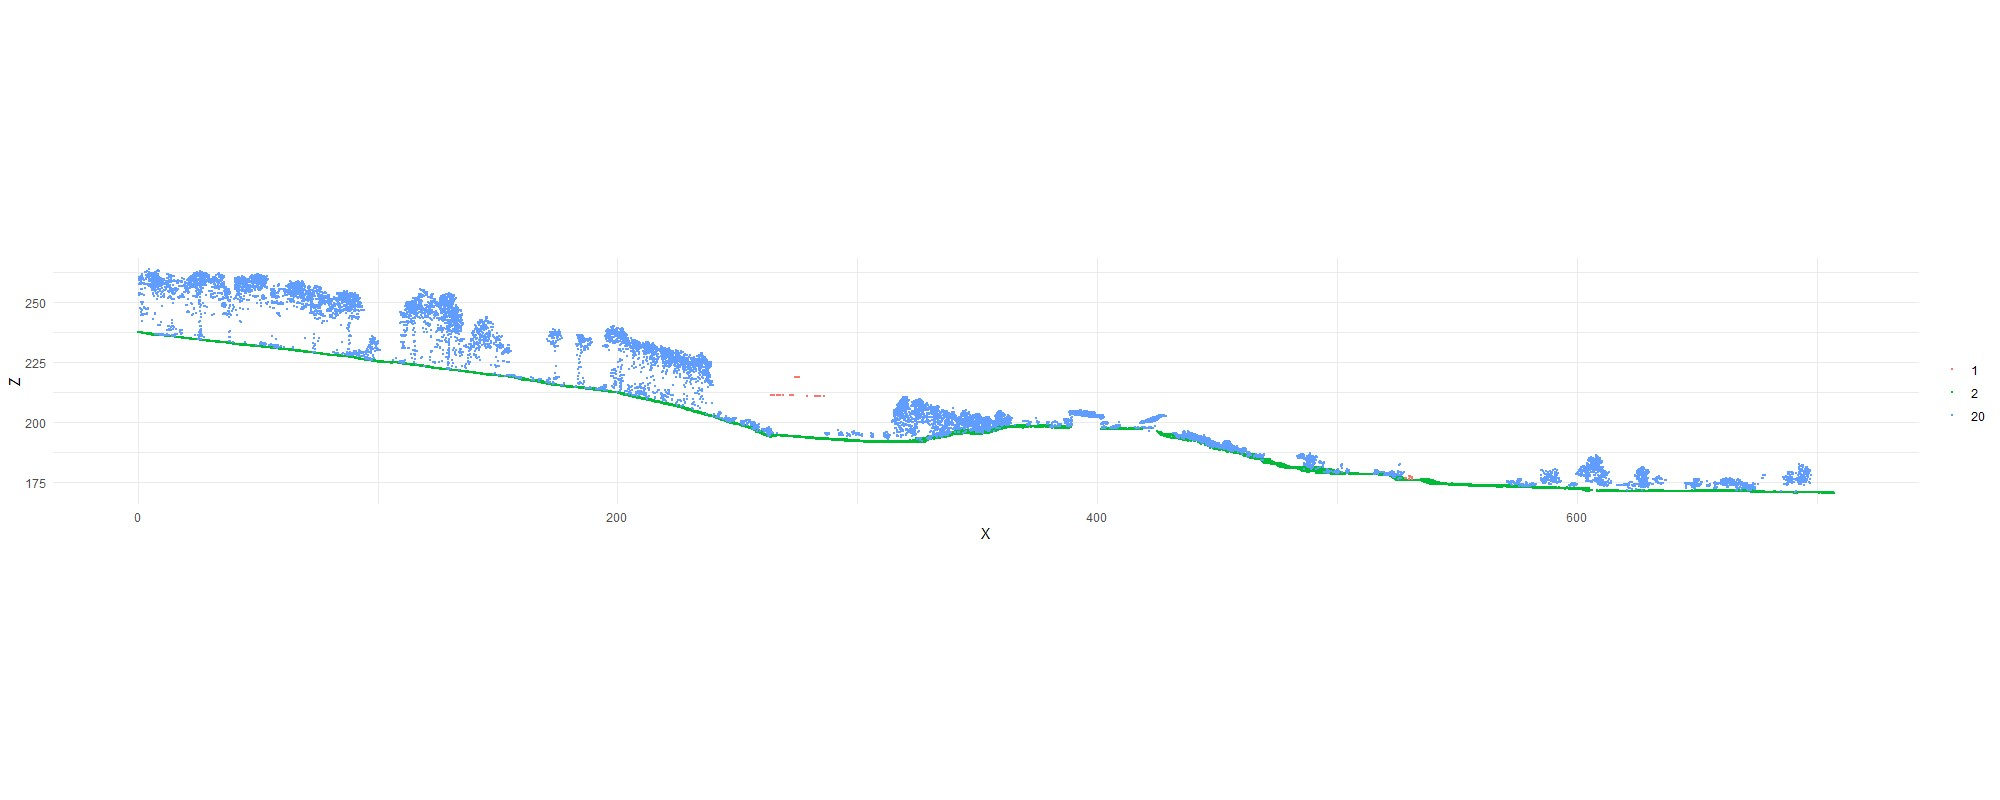
\includegraphics[width=1\linewidth,height=0.7\textheight]{C:/Users/kelto/Documents/iSEGMound/analysis/thesis/figures/Figure_30_1} 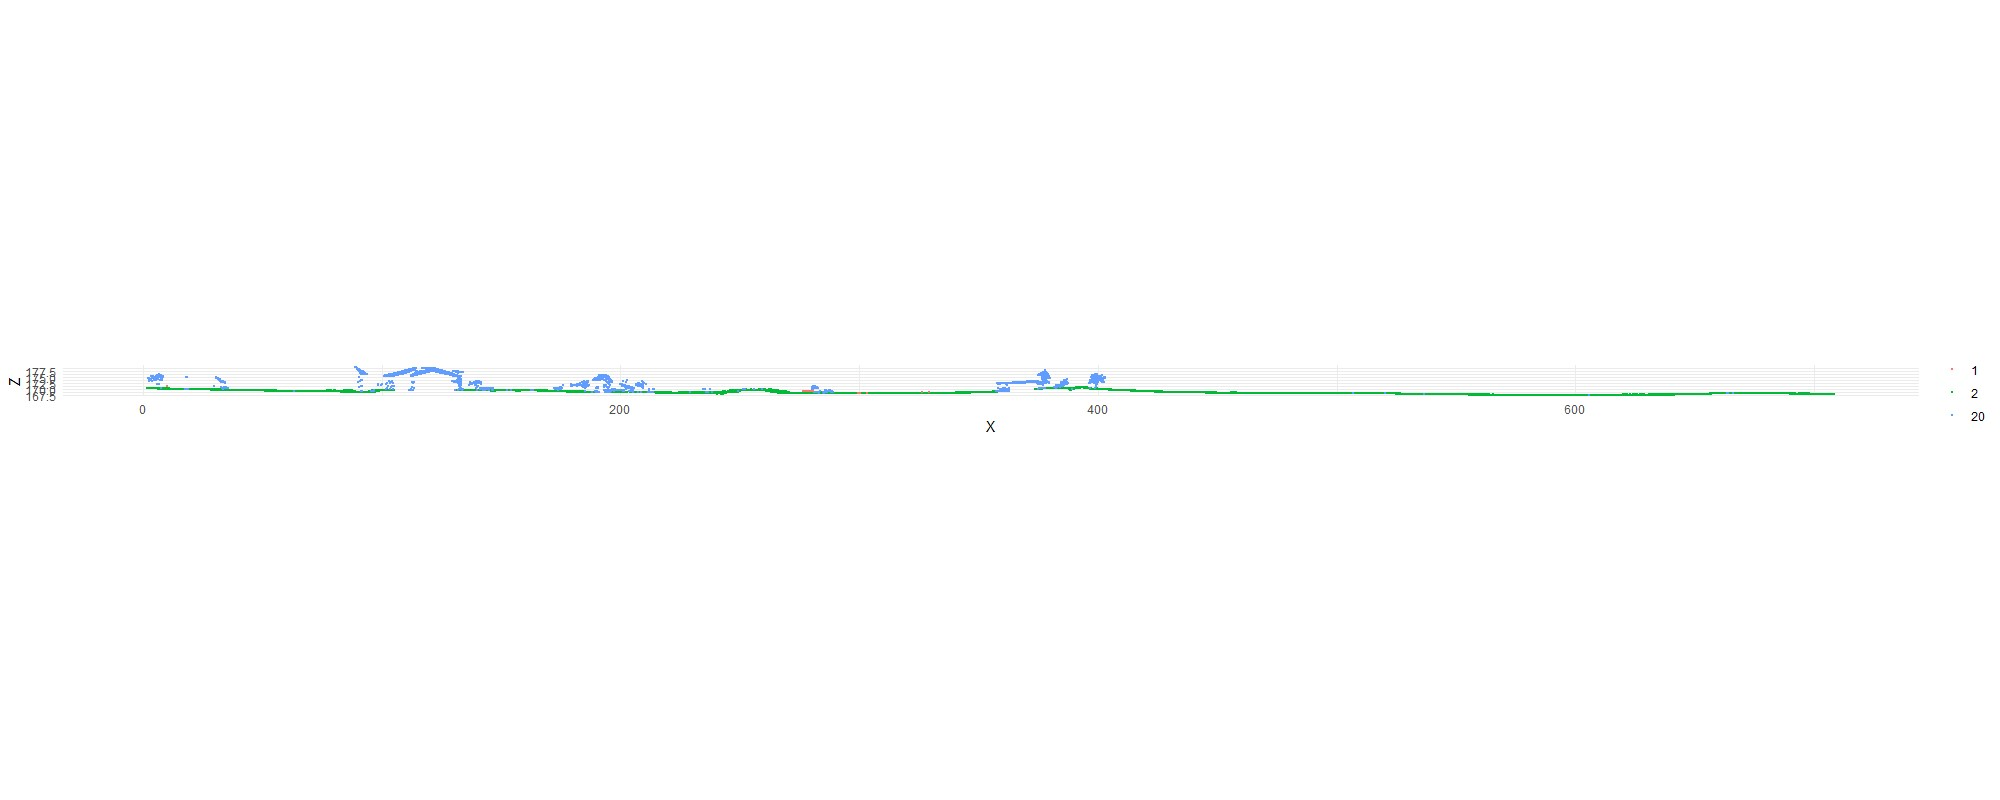
\includegraphics[width=1\linewidth,height=0.7\textheight]{C:/Users/kelto/Documents/iSEGMound/analysis/thesis/figures/Figure_30_2} \caption{Plot of the sections of the ground classification of the test tile.}\label{fig:Figure30}
\end{figure}

Cross sections were plotted for all point re/classifications, but the sections are best observed by zooming in. Thus the cross section plots are depicted in the Supplements (Chapter 9).

\textbf{B) Progressive Morphological Filter (PMF)}
\newline
\textbf{PMF} (Zhang et al.~2003) generates a raster surface from the point cloud which then is processed by multiple morphological operations until stability is reached (Roussel et al.~2020, 4., {[}lidRbook{]} (\url{https://jean-romain.github.io/lidRbook/gnd.html\#pmf}))

\begin{figure}

{\centering 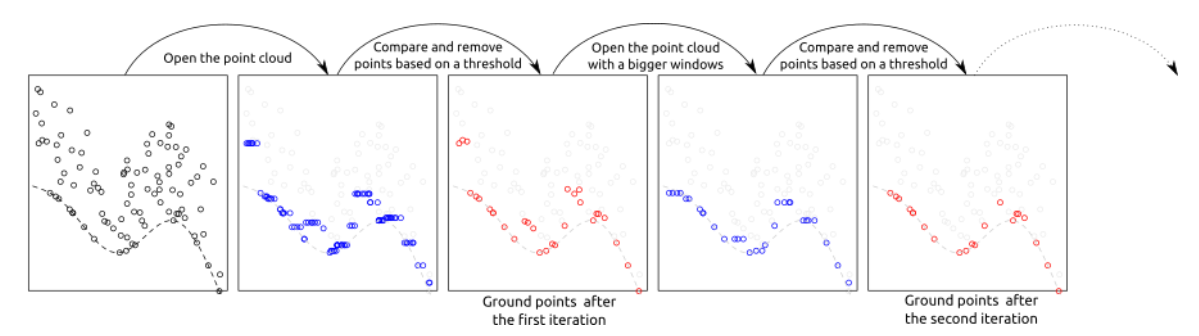
\includegraphics[width=1\linewidth,height=0.7\textheight]{C:/Users/kelto/Documents/iSEGMound/analysis/thesis/figures/Figure_31} 

}

\caption{The workflow of the PMF algorithm.}\label{fig:Figure31}
\end{figure}

Multiple algorithms settings were tested. \texttt{ws} controls the window size of the moving window of the algorithm in meters. \texttt{th} is the threshold for point heights above the ground surface to be considered a ground return, also in meters.

\textbf{\emph{iia LIDR\_200910\_1\_xyzirnc\_pmf}}

\begin{Shaded}
\begin{Highlighting}[]
\NormalTok{LIDR\_200910\_1\_xyzirnc\_pmf }\OtherTok{\textless{}{-}}\NormalTok{ lidR}\SpecialCharTok{::}\FunctionTok{classify\_ground}\NormalTok{(LIDR\_200910\_1\_xyzirnc, }\AttributeTok{algorithm =} \FunctionTok{pmf}\NormalTok{(}\AttributeTok{ws =} \DecValTok{5}\NormalTok{,}
    \AttributeTok{th =} \DecValTok{3}\NormalTok{))}
\end{Highlighting}
\end{Shaded}

\textbf{\emph{iib LIDR\_200910\_1\_xyzirnc\_pmf\_th1}}
\newline
The height threshold was set to 1 m to avoid vegetation and outliers but include scattered ground points:

\begin{Shaded}
\begin{Highlighting}[]
\NormalTok{LIDR\_200910\_1\_xyzirnc\_pmf\_th1 }\OtherTok{\textless{}{-}}\NormalTok{ lidR}\SpecialCharTok{::}\FunctionTok{classify\_ground}\NormalTok{(LIDR\_200910\_1\_xyzirnc, }\AttributeTok{algorithm =} \FunctionTok{pmf}\NormalTok{(}\AttributeTok{ws =} \DecValTok{5}\NormalTok{,}
    \AttributeTok{th =} \DecValTok{1}\NormalTok{))}
\end{Highlighting}
\end{Shaded}

\textbf{\emph{iic LIDR\_200910\_1\_xyzirnc\_pmf\_th05}}
\newline
The height threshold was set to 0.5 m to avoid vegetation and outliers and to approach the ground surface:

\begin{Shaded}
\begin{Highlighting}[]
\NormalTok{LIDR\_200910\_1\_xyzirnc\_pmf\_th05 }\OtherTok{\textless{}{-}}\NormalTok{ lidR}\SpecialCharTok{::}\FunctionTok{classify\_ground}\NormalTok{(LIDR\_200910\_1\_xyzirnc, }\AttributeTok{algorithm =} \FunctionTok{pmf}\NormalTok{(}\AttributeTok{ws =} \DecValTok{5}\NormalTok{,}
    \AttributeTok{th =} \FloatTok{0.5}\NormalTok{))}
\end{Highlighting}
\end{Shaded}

\textbf{\emph{iid LIDR\_200910\_1\_xyzirnc\_pmf\_th005}}
\newline
The height threshold was set to 0.05 m to avoid vegetation and outliers and to get the ground surface as good as possible including possible backscatter of the LiDAR beam. When a height threshold of 0 was chosen, no ground points were (re)classified.

\begin{Shaded}
\begin{Highlighting}[]
\NormalTok{LIDR\_200910\_1\_xyzirnc\_pmf\_th005 }\OtherTok{\textless{}{-}}\NormalTok{ lidR}\SpecialCharTok{::}\FunctionTok{classify\_ground}\NormalTok{(LIDR\_200910\_1\_xyzirnc, }\AttributeTok{algorithm =} \FunctionTok{pmf}\NormalTok{(}\AttributeTok{ws =} \DecValTok{5}\NormalTok{,}
    \AttributeTok{th =} \FloatTok{0.05}\NormalTok{))}
\end{Highlighting}
\end{Shaded}

Comparing the section of \textbf{iid} with a threshold of 5 cm (0.05 m) with the sections of \textbf{iic}, with a threshold of 50 cm (0.5 m) is clearly visible that in the case of \textbf{iid} many of the actual ground points have not been classified as such because of the low threshold.

\textbf{C) Cloth Simulation Function (CSF)}
\newline
\textbf{CSF} (Zhang et al.~2016) simulates a cloth which is dropped on the inverted point cloud and the ground points are classified by analyzing the interactions between the points of the cloth and the inverted surface (Roussel et al.~2020, 5; {[}lidRbook{]} (\url{https://jean-romain.github.io/lidRbook/gnd.html\#csf}))

\begin{figure}

{\centering 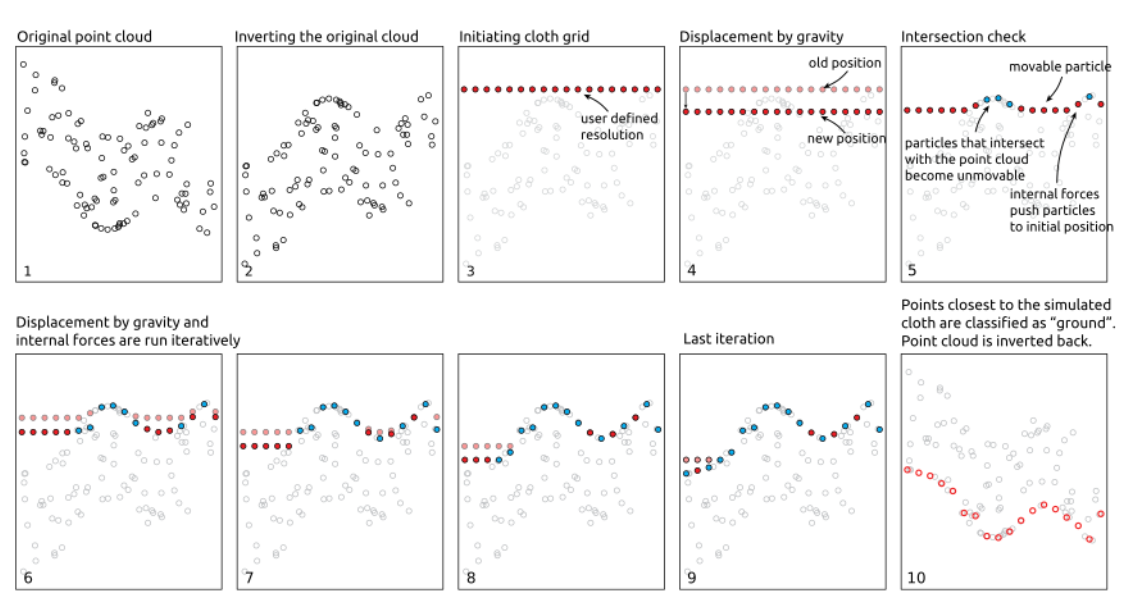
\includegraphics[width=1\linewidth,height=0.7\textheight]{C:/Users/kelto/Documents/iSEGMound/analysis/thesis/figures/Figure_32} 

}

\caption{The workflow of the CSF algorithm.}\label{fig:Figure32}
\end{figure}

\textbf{\emph{iiia LIDR\_200910\_1\_xyzirnc\_csf}}
\newline
First the default settings were tested:

\begin{Shaded}
\begin{Highlighting}[]
\FunctionTok{csf}\NormalTok{(}\AttributeTok{sloop\_smooth =} \ConstantTok{FALSE}\NormalTok{, }\AttributeTok{class\_threshold =} \FloatTok{0.5}\NormalTok{, }\AttributeTok{cloth\_resolution =} \FloatTok{0.5}\NormalTok{, }\AttributeTok{rigidness =}\NormalTok{ 1L,}
    \AttributeTok{iterations =}\NormalTok{ 500L, }\AttributeTok{time\_step =} \FloatTok{0.65}\NormalTok{)}
\end{Highlighting}
\end{Shaded}

Where \texttt{sloop\_smooth=\ TRUE} reduces errors during post-processing; \texttt{class\_threshold} is the distance to the simulated cloth to classify a point cloud into ground and non-ground; \texttt{cloth\_resolution} is the distance between points in the cloth; \texttt{rigidness} stands for the rigidness of the cloth: 1 very soft (to fit rugged terrain), 2 medium, and 3 hard cloth (for flat terrain); \texttt{time\_step} simulates the cloth under gravity. The default value is 0.65 and is suitable for most cases. (\texttt{lidR} vignette for the csf function).

\begin{Shaded}
\begin{Highlighting}[]
\NormalTok{LIDR\_200910\_1\_xyzirnc\_csf }\OtherTok{\textless{}{-}}\NormalTok{ lidR}\SpecialCharTok{::}\FunctionTok{classify\_ground}\NormalTok{(LIDR\_200910\_1\_xyzirnc, }\AttributeTok{algorithm =} \FunctionTok{csf}\NormalTok{())}
\end{Highlighting}
\end{Shaded}

\textbf{\emph{iiib LIDR\_200910\_1\_xyzirnc\_csf2}}
\newline
Because we are interested in depicting the ground surface in detail we are setting \texttt{sloop\_smooth=\ TRUE} and leave the other parameter at default.

\begin{Shaded}
\begin{Highlighting}[]
\NormalTok{csf\_1 }\OtherTok{\textless{}{-}} \FunctionTok{csf}\NormalTok{(}\AttributeTok{sloop\_smooth =} \ConstantTok{TRUE}\NormalTok{, }\AttributeTok{class\_threshold =} \FloatTok{0.5}\NormalTok{, }\AttributeTok{cloth\_resolution =} \FloatTok{0.5}\NormalTok{,}
    \AttributeTok{rigidness =} \DecValTok{1}\NormalTok{, }\AttributeTok{iterations =} \DecValTok{500}\NormalTok{, }\AttributeTok{time\_step =} \FloatTok{0.65}\NormalTok{)}
\NormalTok{LIDR\_200910\_1\_xyzirnc\_csf2 }\OtherTok{\textless{}{-}}\NormalTok{ lidR}\SpecialCharTok{::}\FunctionTok{classify\_ground}\NormalTok{(LIDR\_200910\_1\_xyzirnc, csf\_1)}
\end{Highlighting}
\end{Shaded}

\textbf{\emph{iic LIDR\_200910\_1\_xyzirnc\_csf3}}
\newline
In a last attempt \texttt{rigidness} was set to 2, because the region of Hessen is quite flat but still hilly and thus later we can compare which of the two settings yield better results - also compared to all of the ground segmentation methods.

\textbf{4.3.1.2 Spatial Interpolation}
\newline
In the step before the LAS point cloud has been reclassified (by different methods). In this step the classified points are interpolated to create a terrain model.

Based on the specificities of the Objects of Interest in question, that is the barrows, it is clear that a resolution should be chosen which is detailed enough to also detect small mounds or destroyed ones by plowing, but which is not so high that it results in a big .tif file. Thus first resolutions between 0.5 and 0.05 meters have been tested (0.5, 0.2, 0.1 and 0.05).
A DTM of 0.5 m resolution is between 12,000 and 13,000 KB. A DTM of 0.2 m resolution is between 73,000 and 75,000 KB and a DTM of 0.1 m resolution is between 270,000 and 280,000 KB. If calculating a DTM of 0.05 m = 5 cm resolution, the size of a tile of 1 km is more than 1 GB, which is way too much considering that the 2014 dataset consists of 209 1 km LAS tiles. First the resolution of 0.1 m was chosen, but it had to be realized that without HCP possibility, 0.5m is the best and fastest resolution and option a laptop and a quite good Desktop PC can go processing a rather large dataset.

Three interpolation algorithms are implemented in \texttt{lidR}: Triangulated Irregular Networks (TIN), Inverse Distance Weighing (IDW) and Kriging. In the following the tested settings are demonstrated only on the existing ground classification (\texttt{LIDR\_200910\_1\_ground}).

\textbf{A) Triangulated Irregular Networks (TIN)}
\newline
This algorithm uses the Delaunay triangulation to generate a triangular irregular network from the classified point data. The resulting DTM presents an irregular surface based on non-overlapping triangles. The accuracy depends on the amount and density of points available in the point cloud. The more isolated the points are, the bigger the triangles get thus leading to abrupt elevation changes in the surface and thus to a distorted representation of the ground surface, resulting in edge artifacts.
After testing the resolutions of 0.05, 0.1, 0.2 and 0.5 m, the default settings \texttt{tin()} were used with 0.5m resolution:

\textbf{\emph{iva LIDR\_200910\_1\_ground\_tin05}}

\begin{Shaded}
\begin{Highlighting}[]
\NormalTok{LIDR\_200910\_1\_ground\_tin05 }\OtherTok{\textless{}{-}}\NormalTok{ lidR}\SpecialCharTok{::}\FunctionTok{grid\_terrain}\NormalTok{(LIDR\_200910\_1\_ground, }\AttributeTok{res =} \FloatTok{0.5}\NormalTok{,}
    \AttributeTok{algorithm =} \FunctionTok{tin}\NormalTok{())}
\end{Highlighting}
\end{Shaded}

Subsequently followed by:
\textbf{\emph{ivb LIDR\_200910\_1\_xyzirnc\_pmf\_th03\_tin05}}

\begin{Shaded}
\begin{Highlighting}[]
\NormalTok{LIDR\_200910\_1\_xyzirnc\_pmf\_th03\_tin05 }\OtherTok{\textless{}{-}}\NormalTok{ lidR}\SpecialCharTok{::}\FunctionTok{grid\_terrain}\NormalTok{(LIDR\_200910\_1\_xyzirnc\_pmf\_th03,}
    \AttributeTok{res =} \FloatTok{0.5}\NormalTok{, }\AttributeTok{algorithm =} \FunctionTok{tin}\NormalTok{())}
\end{Highlighting}
\end{Shaded}

\textbf{\emph{ivc LIDR\_200910\_1\_xyzirnc\_pmf\_th1\_tin05}}

\begin{Shaded}
\begin{Highlighting}[]
\NormalTok{LIDR\_200910\_1\_xyzirnc\_pmf\_th1\_tin05 }\OtherTok{\textless{}{-}}\NormalTok{ lidR}\SpecialCharTok{::}\FunctionTok{grid\_terrain}\NormalTok{(LIDR\_200910\_1\_xyzirnc\_pmf\_th1,}
    \AttributeTok{res =} \FloatTok{0.5}\NormalTok{, }\AttributeTok{algorithm =} \FunctionTok{tin}\NormalTok{())}
\end{Highlighting}
\end{Shaded}

\textbf{\emph{ivd LIDR\_200910\_1\_xyzirnc\_pmf\_th05\_tin05}}

\begin{Shaded}
\begin{Highlighting}[]
\NormalTok{LIDR\_200910\_1\_xyzirnc\_pmf\_th05\_tin05 }\OtherTok{\textless{}{-}}\NormalTok{ lidR}\SpecialCharTok{::}\FunctionTok{grid\_terrain}\NormalTok{(LIDR\_200910\_1\_xyzirnc\_pmf\_th05,}
    \AttributeTok{res =} \FloatTok{0.5}\NormalTok{, }\AttributeTok{algorithm =} \FunctionTok{tin}\NormalTok{())}
\end{Highlighting}
\end{Shaded}

\textbf{\emph{ive LIDR\_200910\_1\_xyzirnc\_pmf\_th005\_tin05}}

\begin{Shaded}
\begin{Highlighting}[]
\NormalTok{LIDR\_200910\_1\_xyzirnc\_pmf\_th005\_tin05 }\OtherTok{\textless{}{-}}\NormalTok{ lidR}\SpecialCharTok{::}\FunctionTok{grid\_terrain}\NormalTok{(LIDR\_200910\_1\_xyzirnc\_pmf\_th005,}
    \AttributeTok{res =} \FloatTok{0.5}\NormalTok{, }\AttributeTok{algorithm =} \FunctionTok{tin}\NormalTok{())}
\end{Highlighting}
\end{Shaded}

\textbf{\emph{ivf LIDR\_200910\_1\_xyzirnc\_csf\_tin05}}

\begin{Shaded}
\begin{Highlighting}[]
\NormalTok{LIDR\_200910\_1\_xyzirnc\_csf\_tin05 }\OtherTok{\textless{}{-}}\NormalTok{ lidR}\SpecialCharTok{::}\FunctionTok{grid\_terrain}\NormalTok{(LIDR\_200910\_1\_xyzirnc\_csf,}
    \AttributeTok{res =} \FloatTok{0.5}\NormalTok{, }\AttributeTok{algorithm =} \FunctionTok{tin}\NormalTok{())}
\end{Highlighting}
\end{Shaded}

\textbf{\emph{ivg LIDR\_200910\_1\_xyzirnc\_csf2\_tin05}}

\begin{Shaded}
\begin{Highlighting}[]
\NormalTok{LIDR\_200910\_1\_xyzirnc\_csf2\_tin05 }\OtherTok{\textless{}{-}}\NormalTok{ lidR}\SpecialCharTok{::}\FunctionTok{grid\_terrain}\NormalTok{(LIDR\_200910\_1\_xyzirnc\_csf2,}
    \AttributeTok{res =} \FloatTok{0.5}\NormalTok{, }\AttributeTok{algorithm =} \FunctionTok{tin}\NormalTok{())}
\end{Highlighting}
\end{Shaded}

and:
\newline
\textbf{\emph{ivh LIDR\_200910\_1\_xyzirnc\_csf3\_tin05}}

\begin{Shaded}
\begin{Highlighting}[]
\NormalTok{LIDR\_200910\_1\_xyzirnc\_csf3\_tin05 }\OtherTok{\textless{}{-}}\NormalTok{ lidR}\SpecialCharTok{::}\FunctionTok{grid\_terrain}\NormalTok{(LIDR\_200910\_1\_xyzirnc\_csf3,}
    \AttributeTok{res =} \FloatTok{0.5}\NormalTok{, }\AttributeTok{algorithm =} \FunctionTok{tin}\NormalTok{())}
\end{Highlighting}
\end{Shaded}

\textbf{B) Inverse Distance Weighing (IDW)}
\newline
This algorithm predicts point values based on the spatial distance on known points, during which the nearer points are given larger weights than further ones. This weight is controlled by the parameter p (power). A low p distributes the weights between the nearer and the distant points and thus smoothes the surface. A higher p takes the nearer point stronger in account than the distant ones and can distort the result.

The default setting is:

\begin{Shaded}
\begin{Highlighting}[]
\FunctionTok{knnidw}\NormalTok{(}\AttributeTok{k =} \DecValTok{10}\NormalTok{, }\AttributeTok{p =} \DecValTok{2}\NormalTok{, }\AttributeTok{rmax =} \DecValTok{50}\NormalTok{)}
\end{Highlighting}
\end{Shaded}

where \texttt{k} is the number of the (k-)nearest neighbours, \texttt{p} is the power and \texttt{rmax} is the maximum radius to choose the k-nearest neighbours.

\textbf{\emph{va LIDR\_200910\_1\_ground\_idw05}}
\newline
First the default settings have been tested:

\begin{Shaded}
\begin{Highlighting}[]
\NormalTok{LIDR\_200910\_1\_ground\_idw05 }\OtherTok{\textless{}{-}}\NormalTok{ lidR}\SpecialCharTok{::}\FunctionTok{grid\_terrain}\NormalTok{(LIDR\_200910\_1\_ground, }\AttributeTok{res =} \FloatTok{0.5}\NormalTok{,}
    \AttributeTok{algorithm =} \FunctionTok{knnidw}\NormalTok{(}\AttributeTok{k =}\NormalTok{ 10L, }\AttributeTok{p =} \DecValTok{2}\NormalTok{, }\AttributeTok{rmax =} \DecValTok{50}\NormalTok{))}
\end{Highlighting}
\end{Shaded}

\textbf{\emph{vb LIDR\_200910\_1\_ground\_idw05\_2}}
\newline
Secondly the settings used by \href{https://github.com/gisma/uavRst/wiki/Building-a-Canopy-Height-Model-(CHM)-using-lidR}{Chris} were tested:

\begin{Shaded}
\begin{Highlighting}[]
\NormalTok{LLIDR\_200910\_1\_ground\_idw05\_2 }\OtherTok{\textless{}{-}}\NormalTok{ lidR}\SpecialCharTok{::}\FunctionTok{grid\_terrain}\NormalTok{(LIDR\_200910\_1\_ground, }\AttributeTok{res =} \FloatTok{0.1}\NormalTok{,}
    \AttributeTok{algorithm =} \FunctionTok{knnidw}\NormalTok{(}\AttributeTok{k =}\NormalTok{ 50L, }\AttributeTok{p =} \DecValTok{3}\NormalTok{))}
\end{Highlighting}
\end{Shaded}

\textbf{\emph{vc LIDR\_200910\_1\_ground\_idw05\_3}}
\newline
Thirdly, the default setting have been cut in half for comparison:

\begin{Shaded}
\begin{Highlighting}[]
\NormalTok{LIDR\_200910\_1\_ground\_idw05\_3 }\OtherTok{\textless{}{-}}\NormalTok{ lidR}\SpecialCharTok{::}\FunctionTok{grid\_terrain}\NormalTok{(LIDR\_200910\_1\_ground, }\AttributeTok{res =} \FloatTok{0.5}\NormalTok{,}
    \AttributeTok{algorithm =} \FunctionTok{knnidw}\NormalTok{(}\AttributeTok{k =}\NormalTok{ 5L, }\AttributeTok{p =} \DecValTok{2}\NormalTok{, }\AttributeTok{rmax =} \DecValTok{25}\NormalTok{))}
\end{Highlighting}
\end{Shaded}

\textbf{\emph{vd LIDR\_200910\_1\_ground\_idw05\_4}}
\newline
Fourthly, the default settings have been doubled for comparison - to see how the power influences the smoothness:

\begin{Shaded}
\begin{Highlighting}[]
\NormalTok{LIDR\_200910\_1\_ground\_idw05\_4 }\OtherTok{\textless{}{-}}\NormalTok{ lidR}\SpecialCharTok{::}\FunctionTok{grid\_terrain}\NormalTok{(LIDR\_200910\_1\_ground, }\AttributeTok{res =} \FloatTok{0.5}\NormalTok{,}
    \AttributeTok{algorithm =} \FunctionTok{knnidw}\NormalTok{(}\AttributeTok{k =}\NormalTok{ 20L, }\AttributeTok{p =} \DecValTok{4}\NormalTok{, }\AttributeTok{rmax =} \DecValTok{50}\NormalTok{))}
\end{Highlighting}
\end{Shaded}

\textbf{\emph{ve LIDR\_200910\_1\_ground\_idw05\_5}}
\newline
Fifthly, the default k and p parameters have been multiplied and the radius has been lowered.

\begin{Shaded}
\begin{Highlighting}[]
\NormalTok{LIDR\_200910\_1\_ground\_idw05\_5 }\OtherTok{\textless{}{-}}\NormalTok{ lidR}\SpecialCharTok{::}\FunctionTok{grid\_terrain}\NormalTok{(LIDR\_200910\_1\_ground, }\AttributeTok{res =} \FloatTok{0.1}\NormalTok{,}
    \AttributeTok{algorithm =} \FunctionTok{knnidw}\NormalTok{(}\AttributeTok{k =}\NormalTok{ 50L, }\AttributeTok{p =} \DecValTok{6}\NormalTok{, }\AttributeTok{rmax =} \DecValTok{25}\NormalTok{))}
\end{Highlighting}
\end{Shaded}

he same variable has been applied to the other point-cloud classifications (PMF \& CSF: vf ⎯ ) which is not detailed in this instance but analysed below (Table ).

\textbf{4.3.1.3 Algorithm Comparison and Choice}
\newline
The last step is to compare the generated DTMs to choose which is best representing the actual ground surface and is thus suitable for mound detection. The (point cloud classification and spatial interpolation) algorithms chosen will be applied to the LiDAR data from 2009/2010.

To choose the suitable (point cloud classification and spatial interpolation) algorithms for DTM generation one LAS tile was processed with the different algorithms detailed above. To emphasize the differences between these algorithms a 300 x 250 m section was chosen which features forested and open areas as well as a settlement area. A smaller region of this section (in a red square in Figure 33) is especially important for the algorithm selection, where the understorey of the forest is too dense to be able to let enough laser beams past. In these cases the spatial interpolation algorithm of the classified point cloud is extremely important. The matter is sensitive because the spatial interpolation method has control over the microtopography and geomorphology of the ground surface.

\begin{figure}

{\centering 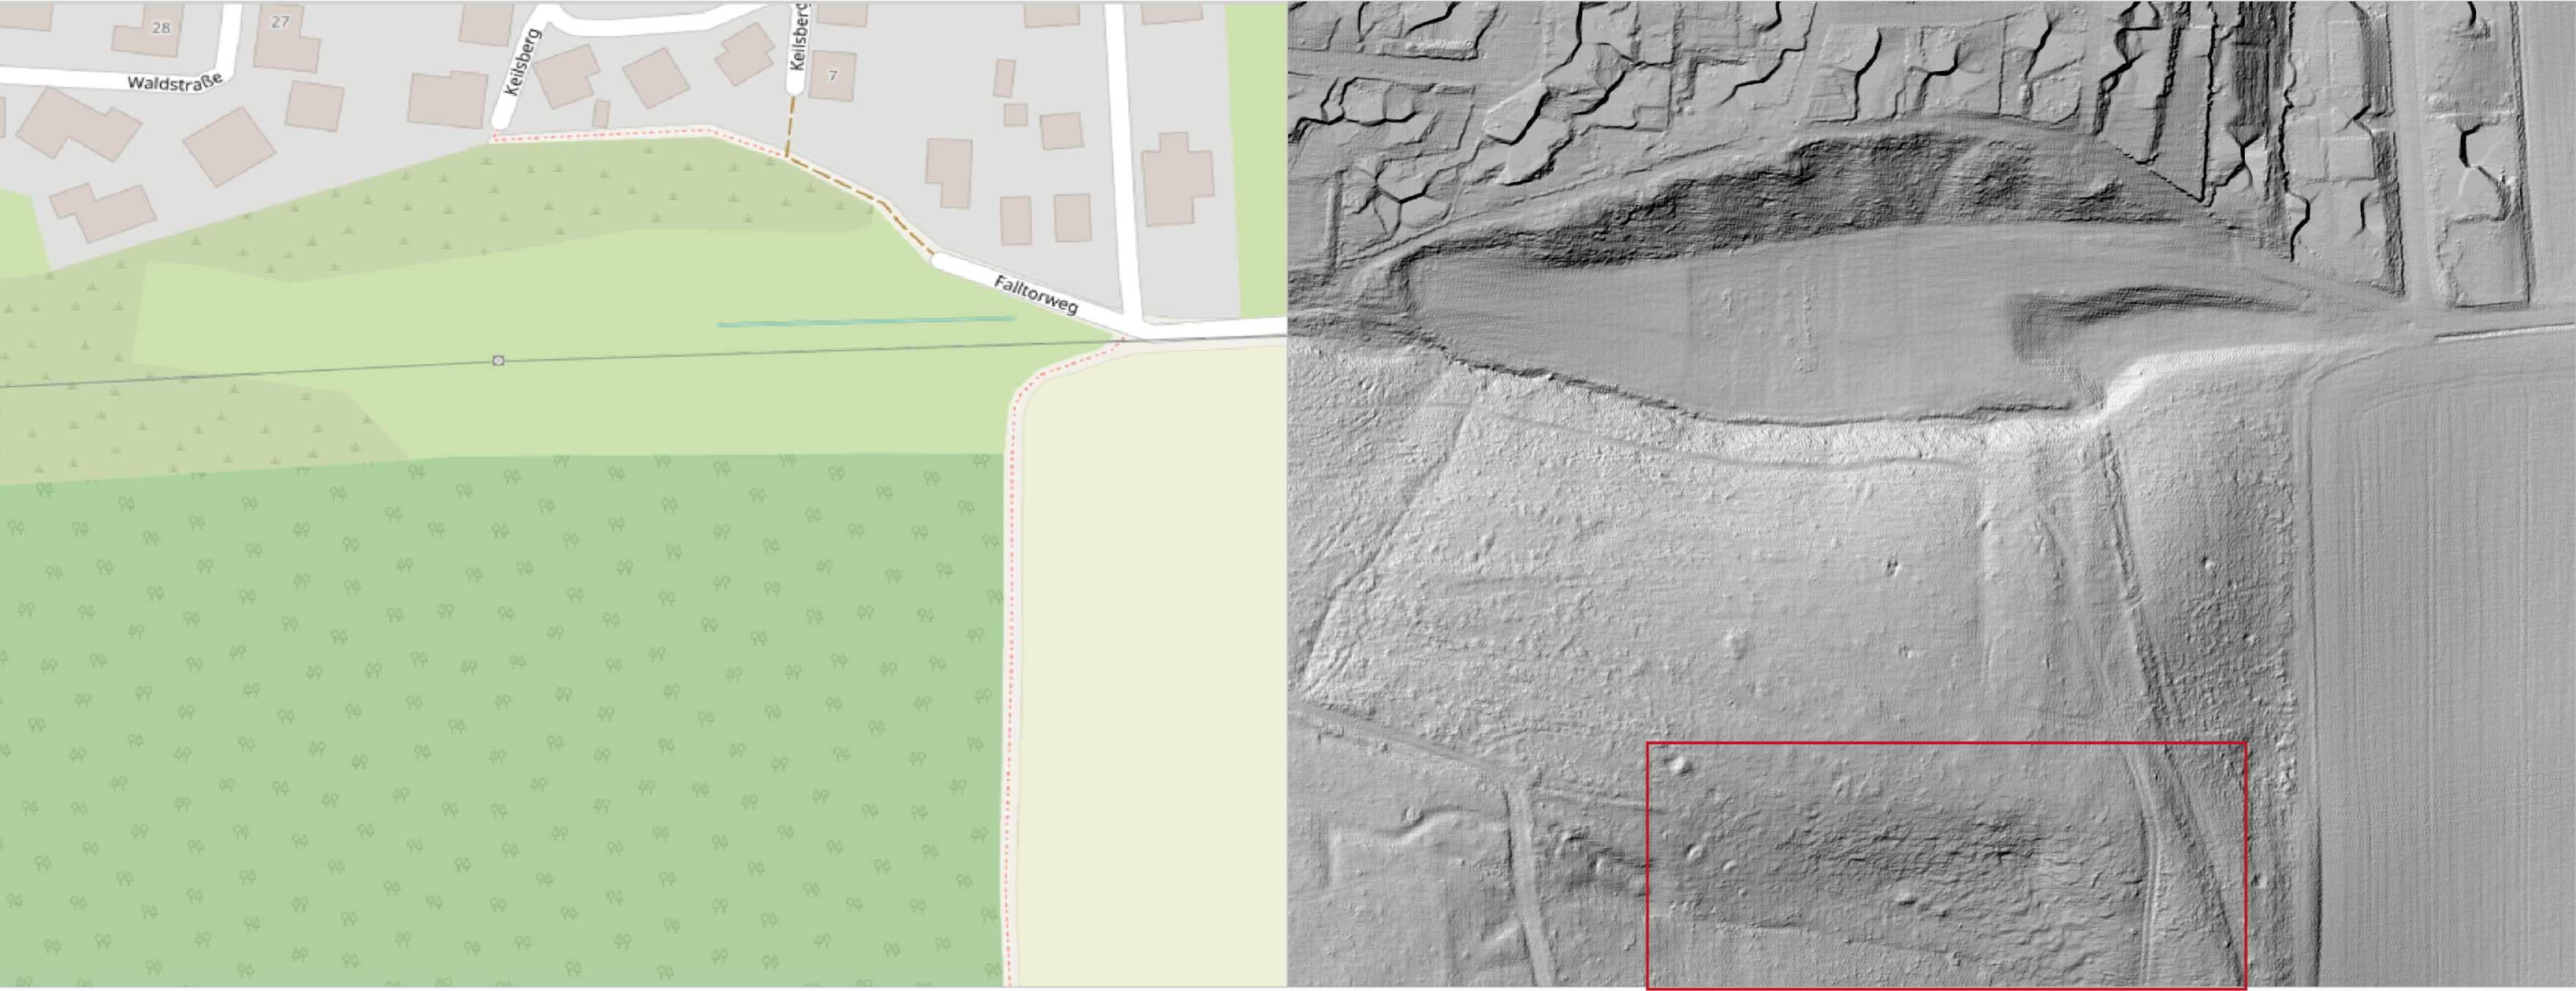
\includegraphics[width=1\linewidth,height=0.7\textheight]{C:/Users/kelto/Documents/iSEGMound/analysis/thesis/figures/Figure_33} 

}

\caption{Comparison of the test section of LAS tile 32478-5616, displayed on OpenStreetMap (left) and ground point classification interpolated by IDW with default settings. A forested area, a field and a meadow, including a settlement is visible. It offers an excellent fundament for algorithm comparison. Scale 1:800.}\label{fig:Figure33}
\end{figure}

The results are compared on two levels: first on point cloud level (point cloud classification) and on raster level (spatial interpolation of the ground points). A summary of the used settings is comprehensible from Table 2.

\begingroup\fontsize{7}{9}\selectfont

\begin{longtable}[t]{lllllll}
\caption{\label{tab:Table2}Summary of the re/classification and interpolation functions and algorithms used.}\\
\toprule
\multicolumn{6}{c}{ POINT CLOUD CLASSIFICATION} & \multicolumn{1}{c}{ } \\
\cmidrule(l{3pt}r{3pt}){1-6}
Progressive Morphological Filter &  &  &  &  &  & \\
 & ws & th &  &  &  & \\
pmf & 5 & 3 &  &  &  & \\
pmf\_th1 & 5 & 1 &  &  &  & \\
pmf\_th05 & 5 & 0.5 &  &  &  & \\
\addlinespace
pmf\_th005 & 5 & 0.05 &  &  &  & \\
Cloth Simulation Function &  &  &  &  &  & \\
 & sloop\_smooth & class\_threshold & cloth\_resolution & rigidness & iterations & time\_step\\
csf & FALSE & 0.5 & 0.5 & 1 & 500 & 0.65\\
csf2 & TRUE & 0.5 & 0.5 & 1 & 500 & 0.65\\
\addlinespace
csf3 & TRUE & 0.5 & 0.5 & 2 & 500 & 0.65\\
SPATIAL INTERPOLATION &  &  &  &  &  & \\
Traingulated Irregular Network (TIN) &  &  &  &  &  & \\
\_tin05 & default &  &  &  &  & \\
Inverse Distance Weighing &  &  &  &  &  & \\
\addlinespace
 & k & p & rmax &  &  & \\
\_idw05 & 10 & 2 & 50 &  &  & \\
\_idw05\_2 & 50 & 3 & 50 &  &  & \\
\_idw05\_3 & 5 & 2 & 25 &  &  & \\
\_idw05\_4 & 20 & 4 & 50 &  &  & \\
\addlinespace
\_idw05\_5 & 50 & 6 & 25 &  &  & \\
\bottomrule
\end{longtable}
\endgroup{}

First of all let's discuss both the Progressive Morphological Filter (PMF) and the Cloth Simulation Function (CSF) algorithms. In the case of the PMF algorithm the size of the moving window (ws) of the algorithm and the height threshold (th) for the points to be classified can be modified. In the case of the CSF algorithm the texture and mass of the cloth/surface can be manipulated with other various parameters (including a class threshold) (see Table 3) Thus both algorithms approach the same from different directions.
For comparison purposes the results are compared according to the spatial interpolation methods used. TIN is implemented with parameter-free Delaunay triangulation and is the most simple linear interpolation method in \texttt{lidR}. The result of the interpolation method is quite clear and thus it is used to highlight the basic differences between the two point cloud classification methods.

Figure 34 shows very clearly that PMF (bottom row) can deal with the artifacts very effectively by changing the height threshold. The threshold heights used were: 3, 1, 0.5, and 0.05 meters. It is clearly visible that heights near the surface (0.5 and 0.05 m) return a very natural ground surface and the perfect value lies somewhere between 0.5 and 0.05 (\texttt{th\ =\ 0.05} purges the surface too much and thus distorts the microtopography). A window size of 5 meters in a 1000 m x 1000 m tile seems reasonably accurate (small enough but not too much) so this parameter has not been changed. It also catches the eye that PMF is the simpler method, being able to control basically only one spatial variable.

\begin{figure}

{\centering \includegraphics[width=1\linewidth,height=0.7\textheight]{C:/Users/kelto/Documents/iSEGMound/analysis/thesis/figures/Figure_34} 

}

\caption{Comparison of different point-cloud classification algorithms using TIN spatial interpolation. Scale 1:800.}\label{fig:Figure34}
\end{figure}

CSF on the other hand already returns with the default settings a quite natural ground surface with only a few (but still crucial) artifacts. There is not much difference if \texttt{sloop\_smooth\ =\ TRUE} or \texttt{FALSE}, but there is a small difference if \texttt{rigidness\ =\ 1} or \texttt{2}, but because the terrain is quite flat the difference is almost invisible.
In the case of PMF and CSF the artifacts on the ground are still existing and thus do not yield better results than spatially interpolating the existing ground classification.
TIN creates strong edges which can deform round objects which are in the focus of this study, thus this method was screened out in favor of IDW.

IDW is more robust to edge artifacts and thus is the preferred interpolation method. As explained previously this interpolation method can be controlled by 3 parameters: \texttt{k} (number of the nearest neighbours involved in the interpolation), \texttt{p} (power) and \texttt{rmax} (the maximum radius to choose the k nearest neighbours from). The value of \texttt{p} steers the influence of points on the interpolation and can lead to smoothed or distorted surfaces. Five different settings were tested (see Table 3 above and Figures 35 to 39, which are displayed in the Supplements).

First the default settings (\texttt{k\ =\ 10,\ p\ =\ 2,\ rmax\ =\ \ 50}) were applied (Figure 35).
Secondly the settings used by Chris were tested (\texttt{k\ =\ 50,\ p\ =\ 3,\ rmax\ =\ 50}, Figure 36).
Thirdly, to test the effect of the number of nearest neighbours, the default settings have been divided in half (\texttt{k\ =\ 5,\ p\ =\ 2,\ rmax\ =\ 25}, Figure 37).
Fourthly, to understand the effect of the number of nearest neighbours and the power even better, the default settings have been doubled, except for \texttt{rmax} (\texttt{k\ =\ 20,\ p\ =\ 4,\ rmax\ =\ 50}, Figure 38.)
Fifthly, the default k and p parameters have been multiplied and the radius has been lowered (\texttt{k\ =\ 50,\ p\ =\ 6,\ rmax\ =\ 25}, Figure 39).

Comparing the settings of IDW05\_2 and IDW05\_5 (\texttt{k\ =\ 50,\ p\ =\ 3,\ rmax\ =\ 50} vs.~\texttt{k\ =\ 50,\ p\ =\ 6,\ rmax\ =\ 25}) it can be said that IDW01\_2 appears more smoothed (bigger radius and half the power) and IDW05\_5 more jagged (same number of neighbours, half the radius and double power) and results in overall distributed artifacts. These effects can be seen in the settlement area and a suffrage in the bottom middle of the test area.
Comparing the settings of IDW05 and IDW05\_3 (\texttt{k\ =\ 10,\ p\ =\ 2,\ rmax\ =\ 50} vs.~\texttt{k\ =\ 5,\ p\ =\ 2,\ rmax\ =\ 25}) it can be said that IDW05\_3 appears more jagged (half the neighbours, half the radius and same power).
The settings of IDW05\_4 (\texttt{k\ =\ 20,\ p\ =\ 4,\ rmax\ =\ 50}) are the double of IDW05 in terms of neighbours and power and appear more jagged than IDW05.

Based on these comparisons, the size of the radius of the \texttt{k} neighbours and the strength of power contributes strongly to the jagged or smooth appearance of an area. The smaller the area to choose the k neighbours from the smaller the variation and thus the ability to flatten a surface and the higher the ruggedness/jaggedness. Also: if the power is stronger in a smaller radius and/or less neighbours, the more jagged the area gets.

Thus the bottom line is that the default settings of IDW05 delivered the most balanced ground surface. At a later point, during the development of the actual workflow - when calculating with the resulting DTMs - it became clear that the resolution had to be decreased to 0.5 meters. The default settings of IDW01 remained the same.

Kriging has not been tested because it took too long for one tile with default settings and thus the 2009/2010 LAZ files would take enormously long to be processed.

This analysis showed that it is possible to look for the perfect settings of point cloud classification and spatial interpolation methods but it is time consuming. The already available ground classification of the LAS format is definitely reliable. The type (in forested areas) and density of the vegetation (especially near the ground surface) and the time of data collection (possibly in a vegetation free period - in the case of the 2009/2010 LAZ files no metadata is available) is very crucial in order to obtain reliable data. In case of blind areas or areas with less points a well-chosen spatial interpolation method can counteract (at least up to a certain degree) the missing information.
For the processing of the LiDAR data sets the ground classification and the IDW spatial interpolation with default settings has been chosen.

\hypertarget{processing-lazlas-data-sets-with-lascatalog}{%
\subsubsection{\texorpdfstring{\textbf{Processing LAZ/LAS Data Sets With LAScatalog}}{Processing LAZ/LAS Data Sets With LAScatalog}}\label{processing-lazlas-data-sets-with-lascatalog}}

The LAScatalog function in lidR enables the user to work with big LAS/LAZ datasets and thus to process large areas, without loading the entire dataset into the computer memory. When working with LAScatalogs, functions can be applied over the entire case study area (batch-processing). Several processing options can be set for the LAScatalog, like chunk processing (splitting the data in multiple part and process them iteratively - sequentially or parallel), creating a buffer around each chunk to ensure output without edge artifacts, merging computed outputs into a single product, logging and return of partial outputs in case of crash, real-time progress estimation monitoring and an error-handling manager (Roussel \emph{et al.} (2020)).

\begin{figure}

{\centering \includegraphics[width=0.7\linewidth,height=0.5\textheight]{C:/Users/kelto/Documents/iSEGMound/analysis/thesis/figures/Figure_35} 

}

\caption{Schematic visualization of the work process of a LAScatalog in lidR. Roussel et al. 2020, 10, Fig 7.}\label{fig:Figure35}
\end{figure}

First the whole case study area was processed as a LAScatalog and exported tile-by-tile, otherwise the Laptop and even the Desktop PC would have flatlined. These 180 tiles were visually investigated and compared to the Liste 1 and 2 of Dobiat et al.~1994, as described in the previous subchapter. The code for this subchapter can be found in script \textbf{3a\_LiDAR\_data\_processing\_catalogue.R}

Based on the identification of the burial mound groups in the DTM the Areas of Interest (AoI 1-5) and the Train Area were chosen. Subsequently each data set of the Areas of Interests and the Train Area was processed as a separate \texttt{LAScatalog} and all tiles were exported separately but also as a single \textbf{.tif} file. The code for the processing of the different Areas of Interests and the Train Area can be find in script
\textbf{3b\_LiDAR\_data\_processing\_AOI\_train\_area\_catalogues.R}

\hypertarget{data-preparation}{%
\subsection{\texorpdfstring{\textbf{Data Preparation}}{Data Preparation}}\label{data-preparation}}

In order to be able to approach the Objects of Interest (OoI), first these have to be prepared by Geometric knowledge-based methods, thus enhanced in relation to their environment by maximizing the contrast between them and their surroundings to generate more coherent areas which are easier to distinguish (for the computer and the human eye). Lately more and more complex methods have been elaborated or endorsed specifically for archaeological use (e.g. Mayoral \emph{et al.} (2017), Orengo \& Petrie (2018), Guyot \emph{et al.} (2018)). Recent studies (Verschoof-van der Vaart \& Landauer (2021), 4) found that it is not always required to prepare the dataset. Thus it was decided to test two approaches: one workflow with data preparation and one without. To find the best suitable data preparation method, all together 91 derivatives were investigated, which can be found in script \textbf{4\_generate\_derivatives.R}. The order of derivatives and methods in the R script does not correspond to the order of methods discussed here, but the numbers correspond. The table displaying all 91 derivatives can be found as a PDF file in the supplementary-materials folder, including also the respective functions which can be used to generate the derivatives, like a quick-guide. In the following a derivative in the PDF is referred to as followed: Openness - \textbf{\emph{Supplement 3/91}}.

First it was checked which native R packages provide functions that can be used for data preparation. Two packages we found to be extremely useful: \texttt{raster} and \texttt{spatialEco}. Furthermore R interfaces exist to external FOSS GIS Software. Amongst others to \textbf{SAGA} (the package \texttt{RSAGA}), \textbf{GRASS GIS} (the package \texttt{rgrass7}) and \textbf{Whitebox GAT} (the package \texttt{whitebox}). Of course not all corresponding methods in all R packages were calculated or worked - it would've been a lot more than 91 derivatives.

A special interest was given to \textbf{morphometric textural analysis and enhancement methods}, because the case study area is slightly hilly with multiple shallow plateaus which are of similar height as the burial mounds (0.38 m to max. 1.2 m, discussed above). Thus in the second approach the attempt is made to enhance and exaggerate the poorly preserved burial mounds by utilizing an appropriate derivative.
In the following, methods are grouped according to the type of transformation the data set has undergone: targeting the raster as a whole or by enhancing only certain areas or regions of the raster. It can be generally said that it is not easy to group data preparation methods because they do overlap in their tools and results and some fit into multiple categories. Thus this grouping cannot and does not try to be conclusive and definitive by any means.

\hypertarget{visualization-methods}{%
\subsubsection{\texorpdfstring{\textbf{Visualization Methods}}{Visualization Methods}}\label{visualization-methods}}

Visualisation methods transform any DTM into derivatives which enhance either physical qualities (LRM) or are of presentational value (\textbf{\emph{Hillshade}}, \textbf{\emph{Openness}}). In this study the former is grouped into \textbf{`morphometric analysis'} (4.4.3) because it represents a morphological transformation of the respective terrain.
Kokalj \& Hesse (2017) discusses 12 visualisation techniques (though they do not make a difference between the presentational and morphometric methods), all processable in the openly available applications \textbf{RVT} and \textbf{LivTool}. Which visualisation method works best, depends on the characteristics of the landscape in question. They deliver best practices to any type of dataset with informative case studies. Apart from the \textbf{\emph{Hillshade}} to visualize the DTMs and the \textbf{\emph{Negative Openness}} - \textbf{\emph{Supplement 3/91}}, no visualisation method with presentational value was calculated, because of the focus on morphometric analyses.

\hypertarget{textural-analysis}{%
\subsubsection{\texorpdfstring{\textbf{Textural Analysis}}{Textural Analysis}}\label{textural-analysis}}

By manipulating cell values in a moving window of a certain size (in our case, because we do look for slight changes in the terrain, at the most 5x5 pixels make sense), the raster layer can be transformed and modulated to fit the needs. This is the basis on which filters work.
Low pass filters work with moving windows and e.g.~calculate the \textbf{\emph{sum}}, the minimum (\textbf{\emph{min}}), the maximum (\textbf{\emph{max}}), the \textbf{\emph{mean}} value, the standard deviation (\textbf{\emph{sd}}) or the most frequent value (\textbf{\emph{modal}}) of all cells in that certain moving window by smoothing it. High-pass filters on the other hand emphasize certain characters of the image, for this they are also called sharpening filters. One example are \textbf{\emph{sobel filters}} which enhance the areas of the image where it's intensity changes, thus detecting edges. They can be calculated in different directions but also combined. Multiple textural analysis methods were tested (Table 3), but the low pass filter proved to be most effective.
The filters in the \texttt{filtR} function (altogether 8 filters) based on work from a previous seminar. Moving window sizes of 3 and 5 pixels were tested (\textbf{\emph{Supplement 3/1-16}}).
Low pass filters are applied in two steps of the general \textbf{iSEGMound workflow}: at the beginning smoothing the DTM/dDTM with a mean filter (based on Freeland \emph{et al.} (2016) and Rom \emph{et al.} (2020)) and before the Segmentation step to generalize and average the pixel values into homogeneous regions to prepare for the Segmentation. In this second case the choice of the suitable filter from the 8 available depends which one creates more homogeneous regions which might differ from data to data.

\begin{longtable}[]{@{}
  >{\raggedright\arraybackslash}p{(\columnwidth - 4\tabcolsep) * \real{0.57}}
  >{\raggedleft\arraybackslash}p{(\columnwidth - 4\tabcolsep) * \real{0.27}}
  >{\raggedleft\arraybackslash}p{(\columnwidth - 4\tabcolsep) * \real{0.16}}@{}}
\caption{Examples of textural analysis methods.}\tabularnewline
\toprule
Derivatives & ID & R package \\
\midrule
\endfirsthead
\toprule
Derivatives & ID & R package \\
\midrule
\endhead
sum, min, max, mean, modal, sd \& sobel filter & \textbf{\emph{Supplement 3/1-16}} & \texttt{raster::} \\
sobal intensity, direction \& edge filter & \textbf{\emph{Supplement 3/47-49}} & \texttt{spatialEco::} \\
Gaussian Smoothing filter & \textbf{\emph{Supplement 3/46}} & \texttt{spatialEco::} \\
Raster Multidimensional Scaling & \textbf{\emph{Supplement 3/34}} & \texttt{spatialEco::} \\
Spherical Variance/Standard Deviation of Surface & \textbf{\emph{Supplement 3/50-51}} & \texttt{spatialEco::} \\
Deviation from trend/minimum/maximum/mean/median/sd & \textbf{\emph{Supplement 3/35-45}} & \texttt{spatialEco::} \\
Max Elevation Deviation local/meso/broad scale & \textbf{\emph{Supplement 3/52-57}} & \texttt{whitebox::} \\
\bottomrule
\end{longtable}

\hypertarget{morphometric-analysis}{%
\subsubsection{\texorpdfstring{\textbf{Morphometric Analysis}}{Morphometric Analysis}}\label{morphometric-analysis}}

Geomorphology and Geomorphometry is a sub-discipline of Geography and morphometric analysis methods are commonly used for various landscape, hydrological and spatial ecological analyses. The morphometric methods processed in this thesis are mainly based on the methods used by Niculiță (2020a).
Among the calculated derivatives are: \textbf{\emph{Slope}}, \textbf{\emph{Aspect}}, \textbf{\emph{Curvature}}, \textbf{\emph{Topographic Position Index}}, \textbf{\emph{Topographic Wetness Index}} and many more (Table 4). These are distinguished from the methods discussed in 4.4.4, because - as some textural analysis methods (the low pass filters) - they target the image as a whole.

\begin{longtable}[]{@{}
  >{\raggedright\arraybackslash}p{(\columnwidth - 4\tabcolsep) * \real{0.36}}
  >{\raggedleft\arraybackslash}p{(\columnwidth - 4\tabcolsep) * \real{0.28}}
  >{\raggedleft\arraybackslash}p{(\columnwidth - 4\tabcolsep) * \real{0.36}}@{}}
\caption{Examples of morphometric analysis methods.}\tabularnewline
\toprule
Derivatives & ID & R package \\
\midrule
\endfirsthead
\toprule
Derivatives & ID & R package \\
\midrule
\endhead
Topographic Position Index & \textbf{\emph{Supplement 3/18, 24}} & \texttt{raster::}/\texttt{spatialEco::} \\
Terrain Ruggedness Index & \textbf{\emph{Supplement 3/17,23,66}} & \texttt{raster::}/\texttt{spatialEco::}/\texttt{RSAGA::} \\
Vector Ruggedness Measure & \textbf{\emph{Supplement 3/25,67}} & \texttt{spatialEco::}/\texttt{RSAGA::} \\
Terrain Surface Convexity & \textbf{\emph{Supplement 3/70}} & \texttt{RSAGA::} \\
Surface Relief Ratio & \textbf{\emph{Supplement 3/30}} & \texttt{spatialEco::} \\
Surface Area Ratio & \textbf{\emph{Supplement 3/31}} & \texttt{spatialEco::} \\
Terrain Surface Texture & \textbf{\emph{Supplement 3/68-69}} & \texttt{RSAGA::} \\
Roughness & \textbf{\emph{Supplement 3/19}} & \texttt{raster::} \\
SAGA WetnessIndex & \textbf{\emph{Supplement 3/90}} & \texttt{RSAGA::} \\
Flowdirection & \textbf{\emph{Supplement 3/22}} & \texttt{raster::} \\
Convergence Index & \textbf{\emph{Supplement 3/60}} & \texttt{RSAGA::} \\
Aspect & \textbf{\emph{Supplement 3/21,72}} & \texttt{raster::}/\texttt{RSAGA::} \\
Slope & \textbf{\emph{Supplement 3/20,71}} & \texttt{raster::}/\texttt{RSAGA::} \\
Hierarchical Slope Position & \textbf{\emph{Supplement 3/33}} & \texttt{spatialEco::} \\
Relative Heights \& Slope Positions & \textbf{\emph{Supplement 3/61-65}} & \texttt{RSAGA::} \\
Dissection & \textbf{\emph{Supplement 3/32}} & \texttt{spatialEco::} \\
Profile Curvature & \textbf{\emph{Supplement 3/26,73}} & \texttt{spatialEco::}/\texttt{RSAGA::} \\
Total Curvature & \textbf{\emph{Supplement 3/27}} & \texttt{spatialEco::} \\
McNab Curvature & \textbf{\emph{Supplement 3/28}} & \texttt{spatialEco::} \\
Boldstad Curvature & \textbf{\emph{Supplement 3/29}} & \texttt{spatialEco::} \\
Morphometric Features & \textbf{\emph{Supplement 3/74-78}} & \texttt{RSAGA::} \\
Upslope/Downslope Curvature & \textbf{\emph{Supplement 3/79-83}} & \texttt{RSAGA::} \\
\bottomrule
\end{longtable}

\hypertarget{morphometric-enhancement-and-extraction-of-specific-features}{%
\subsubsection{\texorpdfstring{\textbf{Morphometric Enhancement and Extraction of Specific Features}}{Morphometric Enhancement and Extraction of Specific Features}}\label{morphometric-enhancement-and-extraction-of-specific-features}}

Points ii-iv and ii-v of the generalized workflow of automated analysis (Figure 28) are discussed together because - as discussed above, the exact differentiation between the methods is often somewhat problematic and subjective.
The first derivative to be inspected is the \textbf{\emph{Local Relief Model}} (LRM \textbf{\emph{Supplement 3/59}}, Table 5), which was developed by Ralf Hesse (Hesse (2010)) and implemented in the FOSS \textbf{LivToolbox} and \textbf{RVT} standalone softwares and subsequently also as an \textbf{ArcGIS Toolbox} (proprietary, by Novák (2014)) and a \textbf{GRASS GIS Add-on} (Petras \& Goddard (2021)). It is basically a purged difference map which is deprived from the big elevation differences and thus leaves only the small elevation differences, where mostly the traces of archaeology are to be found. This already sheds light on why this method was not chosen: it generally enhances the small features but we are interested only in those which are relevant for our Objects of Interest and because of the 0.5 m resolution of the DTM it is better not to enhance the small features. The Local Relief was already used as input derivative by the author of this Master's thesis when using a PBIA approach to archaeological object detection in LiDAR derived DTMs (Schneider (2018a), Schneider (2018b), and Schneider (2019a)) and it became clear, that this special feature of the \textbf{\emph{Local Relief Model}} can be just as much a downfall and distort the results.
\textbf{\emph{Wind Exposition Index}} (\textbf{\emph{Supplement 3/84}}, Table 5) very nicely highlights the burial mounds but also the (hollow-)ways and other structures in the DTM, thus enhancing all structures in the raster at the same time the same way.
Last but not least the \textbf{\emph{Multi-Scale Topographic Index}} (\textbf{\emph{MSTPI or MTPI, Supplement 3/58, 85-89}}, Table 5) has to be discussed. It can be - as also other derivatives - created with different tools; in our case the \texttt{whitebox} and \texttt{RSAGA} R packages were used. It is an integral image approach to measure relative topographic deviation from the mean elevation on micro-, meso- and macro scale (Weiss (2001)) and then to combine these scales into a single multi-band image (in the case of \texttt{whitebox}; the \textbf{SAGA} algorithm produces a single band image), highlighting deviation on all three levels.
Lately Guyot \emph{et al.} (2018) used the FOSS standalone GIS software \textbf{Whitebox GAT} (Lindsay (2016)) to compute first the \textbf{\emph{Maximum Elevation Deviation}} on local-, meso and broad scale (see derivatives in subchapter : 4.4.2, \textbf{\emph{Supplement 3/52-57}}, Table 5). Then, in a second step Guyot \emph{et al.} (2018) created the \textbf{\emph{Multiscale topographic Position Index}} (Lindsay \emph{et al.} (2015)) by a custom R script as an RGB composite. \textbf{Whitebox GAT} and \textbf{Whitebox Tools} can (since then it has been probably implemented) compute the integral image (\textbf{\emph{Multicale Topographic Position Color Composite}}) in a second step (also in the R package \texttt{whitebox}, both authored by Dr.~John Lindsay and his students). This second step did not work in two of the three computer setups (once a stable and clean installation of Ubuntu 18.04 with all dependencies and once a rather messy older Windows 10 installation) which were used during the development of the workflow of this thesis and thus the use of the R package \textbf{whitebox} was abandoned.
As an alternative, the \textbf{\emph{Multi-Scale Topographic Index}} Tool from \textbf{RSAGA/SAGA} was used, which calculates the \textbf{\emph{Topographic Position Index}}, that is the difference of the elevation value of each cell of a DTM and the mean elevation in the radius of a given moving window (Weiss (2001), Jenness (2006)) for different scales and integrates them in one single image.

\begin{longtable}[]{@{}lrr@{}}
\caption{Examples of morphometric enhancement and extraction methods.}\tabularnewline
\toprule
Derivatives & ID & R package \\
\midrule
\endfirsthead
\toprule
Derivatives & ID & R package \\
\midrule
\endhead
Local Relief Model & \textbf{\emph{Supplement 3/59}} & \texttt{rgrass7::} \\
Wind Exposition Index & \textbf{\emph{Supplement 3/84}} & \texttt{RSAGA::} \\
Multiscale Topographic Index & \textbf{\emph{Supplement 3/58}} & \texttt{whitebox::} \\
Multi-Scale Topographic Index & \textbf{\emph{Supplement 3/85-89}} & \texttt{RSAGA::} \\
\bottomrule
\end{longtable}

The difference between the two \textbf{\emph{Multi-Scale Topographic Index}} calculations is that \texttt{whitebox} works with the \textbf{\emph{maximum elevation deviation}} and \texttt{R/SAGA} works with the \textbf{\emph{mean elevation deviation}}. The results of the computation of the \texttt{R/SAGA} tool are not that straight forward, but still fit the need: they exaggerate the burial mounds and suppress the background enough, thus this morphometric method was used as data Geometric knowledge-based data preparation method.

\hypertarget{data-analysis}{%
\subsection{\texorpdfstring{\textbf{Data Analysis}}{Data Analysis}}\label{data-analysis}}

The steps undertaken until now prepared the data to be manipulated by specific methods and algorithms, but did not change the data in such great length.
As already mentioned, different data and research questions call for different methods. Therefore the respective workflows chosen as paragons based on their good description in the published studies \textbf{iMound} - Freeland \emph{et al.} (2016), Davis \emph{et al.} (2019), Rom \emph{et al.} (2020)) and their reproducibility (\textbf{Watershed Segmentation} - Niculiță (2020a)), the methods \textbf{Geometric knowledge-based Analysis} (iii-i/IV.5.1) and \textbf{GeOBIA} (iii-ii/IV.5.2) are elaborated (Figure 28).

\hypertarget{geometric-knowledge-based-analysis}{%
\subsubsection{\texorpdfstring{\textbf{Geometric Knowledge-Based Analysis}}{Geometric Knowledge-Based Analysis}}\label{geometric-knowledge-based-analysis}}

The most interesting and well-documented Geometric knowledge-based method for object-extraction is \textbf{iMound}, which was developed by Freeland \emph{et al.} (2016) (the predecessor of the use of the pit-filling algorithm itself was Hanus \& Evans (2016) who used \textbf{ArcGIS}), then applied by Davis \emph{et al.} (2019) and lately by Rom \emph{et al.} (2020). In the following these precedent methods are shortly described and illustrated by workflows created in R.

\textbf{4.5.1.1 Freeland \emph{et al.} (2016)} \textbf{\emph{iMound}}
\newline
The workflow (Figure 41) was developed to detect monumental earthworks in LiDAR data on Tonga in West Polynesia. The main point to emphasize is that the objects are clearly better preserved (the mound height was not discussed, but the threshold for minimum mound height was 1 m), than the mounds in the case study area of this thesis. This made it clear that the workflow is not completely transferable, because every site and the archaeological objects in that landscape has its specificity. From the study it is clear that the \textbf{iMound} algorithm was implemented in \texttt{R}, but the details (which package was used and which function) were not disclosed. Following Freeland \emph{et al.} (2016) the \textbf{pit-filling algorithms} by Planchon \& Darboux (2002) and Wang \& Liu (2006) (implemented in SAGA and used through \texttt{RSAGA} in \texttt{R}) were tested for the thesis. The Planchon \& Darboux (2002) algorithm was a lot slower than the Wang \& Liu (2006) algorithm, thus it was decided to use that for the Master's thesis. Present thesis mainly kept to this workflow.

\begin{figure}

{\centering \includegraphics[width=1\linewidth,height=1\textheight]{C:/Users/kelto/Documents/iSEGMound/analysis/thesis/figures/Figure_36} 

}

\caption{The reconstructed workflow of Freeland et al. 2016.}\label{fig:Figure36}
\end{figure}

\textbf{4.5.1.2 Davis \emph{et al.} (2019)} \textbf{\emph{SD}}
\newline
This workflow starts directly with the inversion of the raster and uses a different depression mapping analysis - \textbf{Stochastic Depression Analysis (SDA)}, implemented in \textbf{Whitebox GAT} (the standalone FOSS GIS)(Figure 42). The authors refer to the workflow of Freeland \emph{et al.} (2016) but they don't elucidate why they chose SDA over the fill-sink method exactly. It is only implied by describing the benefit of SDA to highlight small elevation changes (Davis \emph{et al.} (2019), 168) and that the \textbf{Monte Carlo Simulation} incorporates the assumption for topographic uncertainty (Davis \emph{et al.} (2019), 169).

\begin{figure}

{\centering \includegraphics[width=1\linewidth,height=1\textheight]{C:/Users/kelto/Documents/iSEGMound/analysis/thesis/figures/Figure_37} 

}

\caption{The reconstructed workflow of Davis et al. 2019.}\label{fig:Figure37}
\end{figure}

\textbf{4.5.1.3 Rom \emph{et al.} (2020)} \textbf{\emph{iMound}}
\newline
This description of the approach of \textbf{iMound} in this study has the most similarity to a workflow: a pictorial depiction of the different steps (Rom \emph{et al.} (2020), 254, Figure 254). It is not specified which lowpass filter was used. Similarly: although the \textbf{pit filling algorithm} of Wang \& Liu (2006) was used as in Freeland \emph{et al.} (2016), it was not specified which software and tool or function was used. The only difference to Freeland \emph{et al.} (2016) is that the results of the \textbf{iMound} include the inversion of the results (Figure 43). The minimum threshold for mound height is also in this case 1 m, which is, as already mentioned before in subchapter 4.5.1.1, higher than most of the burial mound in the Master's thesis (which are often only slightly different from the major morphological forms of the terrain), thus a different approach than setting a height threshold was approached to extract and effectively detect burial mounds.

\begin{figure}

{\centering \includegraphics[width=1\linewidth,height=1\textheight]{C:/Users/kelto/Documents/iSEGMound/analysis/thesis/figures/Figure_38} 

}

\caption{The reconstructed workflow of Rom et al. 2020.}\label{fig:Figure38}
\end{figure}

\hypertarget{geobia}{%
\subsubsection{\texorpdfstring{\textbf{GeOBIA}}{GeOBIA}}\label{geobia}}

The most recent and only reproducible \textbf{GeOBIA} workflow is Niculiță (2020a). Although not completely reproducible because the underlying data set is not freely available but can be requested from the author by signing a contract for data use. The ideal reproducible code and workflow also includes a \textbf{Docker} file with the exact computational environment in which the published results were created. Latter fact does not detract from the value of the study.
The code starts with the statement ``The self-explanatory R script\ldots{}'' and although it starts with the computation of local peaks and terminates with a random forest classification, the main part consists of concatenated \textbf{SAGA} tools without much comments. It might take some time to understand what the steps in the workflow do, even with having a detailed workflow (Niculiță (2020a), Figure 5; Figure 39). It is hard to look up the documentation of the different \textbf{SAGA} tools, because they are called differently compared to the sections in the code. In addition, when using the RSAGA package with the most recent SAGA version, the following warning results: ``\emph{You seem to be using SAGA GIS 7.9.0, which may cause problems due to changes in names and definitions of SAGA module arguments, etc.}'' As \texttt{RSAGA} requires \textbf{SAGA GIS} versions 2.3.1 LTS - 6.2.0, it means that only functions existing in those versions can be called in R and not functions in your installed SAGA version if it is higher than the requirement (in the case of this thesis SAGA GIS 7.9.0). It would've been useful to note this in the script. Still, \texttt{RSAGA} is working a lot more robust on Windows and Linux and this is why it was chosen instead of \texttt{whitebbox} for the calculation the \textbf{\emph{Multi-Scale Topographic Index}} derivative.
A schematic flowchart of the main general steps would've been useful and although the steps using different software types and the data types are color \& shape coded, still the boxes have different sizes which can make a less experienced reader think that the steps have different significance. Although it is a good idea to want to put as much information in a workflow, it makes this workflow especially overcrowded and too colorful, also because multiple shades of a color are used. The illustrated steps in Niculiță 2020, Figure 6 counterbalance this.

\begin{figure}

{\centering \includegraphics[width=1\linewidth,height=1\textheight]{C:/Users/kelto/Documents/iSEGMound/analysis/thesis/figures/Figure_39} 

}

\caption{Workflow of Niculita 2020, Figure 5.}\label{fig:Figure39}
\end{figure}

The idea of peak extraction is a resourceful geometric knowledge-based method, which works better in a flatter area than in the case study area of this thesis. The \textbf{peak extraction} was tested on the train DTM with 3x3 and 5x5 moving window. Latter window size, that is a search area of 25 pixels still generated too many peaks per segment, and the use of a bigger search radius would've needed a much bigger screen. Thus the peak search approach was abandoned but the \textbf{Watershed Segmentation} step was adapted.

\hypertarget{isegmound}{%
\subsubsection{\texorpdfstring{\textbf{iSEGMound}}{iSEGMound}}\label{isegmound}}

The developed workflow in this thesis is based on the \textbf{iMound} workflow, but because the OoI, that is the burial mounds are preserved very minimally (in general less than 0.5 m), a work-around had to be found to distinguish the shallow mounds from the shallow terrain elevations which would result in the same height. Thus there was no sense to filter the result for height. This is also the reason why peak-search would've resulted in too much information (points) to be filtered out. The workaround consisted in segmenting the areas which were extracted by the \textbf{iMound} workflow and then to filter for shape indices of the mounds in the Train DTM/Train Area. Thus \textbf{Geometric knowledge-based Analysis} and \textbf{GeOBIA methods} are used in the workflow of the thesis.
Before going into more detail about the workflow a schematic workflow is accentuating the main steps (Figure 40):

\begin{figure}

{\centering \includegraphics[width=0.5\linewidth,height=0.5\textheight]{C:/Users/kelto/Documents/iSEGMound/analysis/thesis/figures/Figure_40} 

}

\caption{Scheme of the iSEGMound workflow including data preprocessing.}\label{fig:Figure40}
\end{figure}

In the case of the \textbf{iMound} workflow, mainly Freeland \emph{et al.} (2016) was followed, apart from the thresholding. Regarding the segmentation, two segmentation algorithms were tested: \textbf{Watershed} and \textbf{Region Growing} (both detailed in Chapter 2). During the calculation of the derivatives (Chapter 4.4) it was found that \textbf{\emph{Multi-Scale Topographic Position Index}} (from there on \textbf{\emph{MSTPI}}) does really enhance the homogeneity of the hardly visible burial mounds in arable land and suppresses the rugged microtopography created by the Spatial Interpolation of the Ground point classification. This is not so striking at first glance in the case of the \texttt{RSAGA/SAGA} algorithm but it is visible when zooming in and it is ``enough'' for the segmentation.
In this Master's thesis two data preparation methods (no data preparation and \textbf{\emph{MSTPI}} as explained in Chapter 4.4) and two segmentation methods were used and compared. Using the Training DTM (\textbf{1 tile; scripts 5a to 5d}) it was soon realized that the optimal values used in the segmentation algorithms change with the size of the area, thus all 4 workflows were computed also for the Training Area (\textbf{5 tiles; scripts 6a to 6d}). This means that eight workflows were created and calculated, which include workflows for smaller and for bigger areas. To test the feasibility of the values, a workflow was chosen from the workflows adapted to the Training Area, based on statistical comparison of the segmentation results (explained and detail in Chapter 5.). This chosen workflow was then tested on 5 Areas of Interest (\textbf{AoI 1, AoI 2, AoI 3, AoI 4, AoI 5}). The results will be discussed in Chapter 5.

Because the same workflow was used altogether 13 times and thus certain processes or tools were used frequently, certain functions were written. There are also some borrowed functions.

\texttt{plot\_crossection}: is borrowed from the \href{https://jean-romain.github.io/lidRbook/io.html\#plot}{lidR cookbook}
\newline
\texttt{create\_regions}: was found on \href{https://gis.stackexchange.com/questions/79114/joining-nearest-neighbor-small-polygons-using-r}{stackexchange}
\newline
\texttt{filtR}: was transformed function from a biodiversity seminar course

All the other functions are wrapper functions for SAGA tools, available in the RSAGA package:
\newline
\texttt{generate\_mtpi\_SAGA}: wrapper around the \href{http://www.saga-gis.org/saga_tool_doc/7.9.1/ta_morphometry_28.html}{RSAGA:: ta\_morphometry 28 tool}
\newline
\texttt{fill\_sink\_SAGA\_WL}: wrapper around the \href{http://www.saga-gis.org/saga_tool_doc/7.9.1/ta_preprocessor_4.html}{RSAGA:: ta\_preprocessor 4 tool}
\newline
\texttt{watershed\_segmentation\_SAGA}: wrapper around the \href{http://www.saga-gis.org/saga_tool_doc/7.9.1/imagery_segmentation_0.html}{RSAGA:: imagery\_segm 0 tool}
\newline
\texttt{generate\_seeds\_SAGA}: wrapper around the \href{http://www.saga-gis.org/saga_tool_doc/7.9.1/imagery_segmentation_2.html}{RSAGA:: imagery\_segm 2 tool}
\newline
\texttt{seeded\_region\_growing\_SAGA}: wrapper around the \href{http://www.saga-gis.org/saga_tool_doc/7.9.1/imagery_segmentation_3.html}{RSAGA:: imagery\_segm 3 tool}
\newline
\texttt{polygonize\_segments\_SAGA}: wrapper around the \href{http://www.saga-gis.org/saga_tool_doc/7.9.1/shapes_grid_6.html}{RSAGA:: shapes\_grid 6 tool}
\newline
\texttt{compute\_shape\_index\_SAGA}: wrapper around the \href{http://www.saga-gis.org/saga_tool_doc/7.9.1/shapes_polygons_7.html}{RSAGA:: shapes\_polygons 7 tool}

The \textbf{iSEGMound workflow} (Figure 41) consists of the following steps:

\textbf{Step 0)} \textbf{\emph{Data preprocessing}}
\newline
The data pre-processing was done with the \texttt{lidR\ package} (Roussel \emph{et al.} (2020)) and is described in Chapter 4.3. The corresponding R scripts are: \textbf{2\_LiDAR\_data\_processing\_tile\_1.R}, \textbf{3a\_LiDAR\_data\_processing\_catalogue.R}, \textbf{3b\_LiDAR\_data\_processing\_AOI\_catalogues.R}.

\textbf{Step 1)} \textbf{\emph{Data preparation}}
\newline
The input raster is prepared either by the morphometric enhancement of burial mounds (Chapter 4.4.4) using the \texttt{generate\_mtpi\_SAGA} wrapper creating a \textbf{\emph{MSTPI}}. The algorithm originates from Guisan \emph{et al.} (1999) and Weiss (2001) and was implemented by Lindsay \emph{et al.} (2015) in \textbf{Whitebox GAT} and then applied by Guyot \emph{et al.} (2018). The algorithm used in the thesis is tool 28 from the \textbf{SAGA Morphometry toolbox}. Alternatively the DTM serves input raster.

\textbf{Step 2)} \textbf{\emph{iMound}}
\newline 
\textbf{2a)} A \textbf{\emph{mean filter}} is applied on the input raster (\textbf{\emph{DTM/MSTPI}}) using the \texttt{filtR} wrapper function. The moving window was set to 3x3, because the Object of Interests (mounds) are represented quite shallow and we want to preserve delicate features but also profit form the filter function.
\newline
\textbf{2b)} To invert the filtered raster the \texttt{spatialEco::raster.invert} function is used. The equation implemented in this function in the \texttt{spatialEco} R package is the same as used Davis \emph{et al.} (2019).
\newline
\textbf{2c)} Using the \textbf{pit filling algorithm} by Wang \& Liu 2006 in the \texttt{fill\_sink\_SAGA\_WL} wrapper form, following Freeland \emph{et al.} (2016) and Rom \emph{et al.} (2020).
\newline
\textbf{2d)} The pit-filled inverse raster is subtracted from the inverse raster.

The results contain the burial mounds but also a lot of other objects and information. This result is segmented in the third step.

\textbf{Step 3)} \textbf{\emph{Segmentation}}
\newline
\textbf{3a)} As a pre-processing method for the segmentation, the input raster of the segmentation is filtered with the different implemented filters: \textbf{\emph{sum}}, \textbf{\emph{min}}, \textbf{\emph{max}}, \textbf{\emph{mean}}, \textbf{\emph{median}}, \textbf{\emph{modal}}, \textbf{\emph{sd}} and \textbf{\emph{sobel}} to enhance the burial mounds even more. Freeland \emph{et al.} (2016), 69 mention a secondary filtering after the \textbf{iMound workflow}, thus this was tested out, computing all filters implemented in the \texttt{filtR} wrapper function. The filtered results were then checked in QGIS and compared to each other to choose the filter which prepares and exaggerates the mounds best for the segmentation. The chosen filter can be seen in the respective R scripts.
\newline
\textbf{3b-i)} \textbf{Watershed Segmentation}
\newline
The \texttt{watershed\_segmentation\_SAGA} wrapper is used, following Niculiță (2020a).
\newline
\textbf{3b-ii)} \textbf{Seeded Region Growing Segmentation}
\newline
\textbf{3b-ii-a)} First seed points have to be generated for the next step using the \texttt{generate\_seedpoints\_SAGA} wrapper.
\newline
\textbf{3b-ii-b)} These seed points are then used by the \texttt{region\_growing\_SAGA} wrapper to generate segments. To have a measure of goodness (not in the statistical way), \textbf{Seeded Region Growing} was implemented as an alternative segmentation method. \textbf{Region Growing Segmentation}, contrary to the \textbf{Watershed Segmentation}, is a bottom-up method and this contrast makes the two segmentation methods perfect for comparison.
\newline
\textbf{3c)} The segmentation resulting from \textbf{3b-i)} and \textbf{3b-ii-b)} are raster, thus these have to be polygonized by the wrapper \texttt{polygonize\_segments\_SAGA} to transform the segments to polygons.
\newline
\textbf{3d)} The polygonization is followed by joining touching segments together by the \texttt{create\_regions} function, adapted from stackexchange.
\newline
\textbf{3d-i)} In the case of \textbf{Region Growing Segmentation} also the background was segmented, resulting in huge segments, thus before joining neighbouring segments, these big segments have to be purged. This can be done by plotting the segment with mapview and checking the ID of the big segments and then subset the segments by subtracting them.\\
\newline
\textbf{3e)} After polygonization (and occasional purging from bigger segments created by \textbf{Region Growing Segmentation}), the \textbf{Shape Indices} of the segments are computed using the wrapper function \texttt{compute\_shape\_index\_SAGA}.
\newline
\textbf{3f)} Additionally to the indices implemented in the \textbf{SAGA tool} three indices used by Niculiță (2020a) are implemented (\emph{compactness}, \emph{roundness}, \emph{elongation}).

\textbf{Step 4)} \textbf{\emph{Thresholding}}
\newline
\textbf{4a)} A shapefile (mask) containing the known burial mounds of the \textbf{Training DTM} or the \textbf{Training Area} is loaded and overlaid on the segments resulting from the segmentation. The segments which comply with the mask are filtered and their \textbf{Shape Indices} (descriptors) are documented (a minimum to maximum range is recorded). Thus the threshold will not be set on basis of the ``template''/optimal burial mounds, but on mounds which reflect ``natural'' features (will be elaborated in Chapter 5).
\newline
\textbf{4b)} As the last step the segmentation results are filtered for segments which have similar minimum to maximum descriptor range as the segments complying to the burial mound mask.

\textbf{Step 5)} \textbf{\emph{Verification of results}}
\newline
This covers the comparison of the results of the thresholding to the Train DTM, the Train Area and AoI 1-5 with the burial mounds mapped by Dobiat \emph{et al.} (1994).

The complete workflow can be inspected in Figure 41:

\begin{figure}

{\centering \includegraphics[width=0.7\linewidth,height=0.7\textheight]{C:/Users/kelto/Documents/iSEGMound/analysis/thesis/figures/Figure_41} 

}

\caption{The detailed iSEGMound workflow.}\label{fig:Figure41}
\end{figure}

All scripts are commented and instructions are given in the appropriate place. The comparison of the two segmentation methods is discussed in Chapter 5.

\newpage

\vspace{5mm}
\justifying

\hypertarget{results-of-the-isegmound-workflow}{%
\section{Results of the iSEGMound Workflow}\label{results-of-the-isegmound-workflow}}

In this Master's thesis two data preparation methods (using a plain DTM vs.~a \textbf{\emph{MSTPI}}, as described an explained in Chapter 4) and two segmentation methods (\textbf{Watershed} and \textbf{Region Growing}, as described in Chapter 2 and explained in Chapter 4) were examined, applied and compared, resulting in four workflows. The basic settings and the exact structure and process for the four workflows were tested and debugged on the Train DTM (one 1x1 km tile) and then applied and to the Train Area (five 1x1 km tile) to understand the relationship between the size of the area of investigation and the variable settings of the respective algorithms. These settings were the adjusted and the most effective workflow was chosen (based on the Train Area). This was followed by the application of the selected workflow to the five Areas of Interests (AoI): \textbf{AoI 1, AoI 2, AoI 3, AoI 4 and AoI 5}.

First let's inspect the chosen morphometric derivative, the \textbf{\emph{MSTPI}}, on the example of the Train DTM (Figure 42). The burial mounds of Site ID 5 are clearly discernable and with a closer look also Site ID 35-1. As a reminder let's overlay the burial mound groups \textbf{Site ID 5 (black)} and Site \textbf{ID 35-1 (blue)}:

\begin{figure}
\includegraphics[width=0.5\linewidth,height=0.5\textheight]{C:/Users/kelto/Documents/iSEGMound/analysis/thesis/figures/Figure_42_1} \includegraphics[width=0.5\linewidth,height=0.5\textheight]{C:/Users/kelto/Documents/iSEGMound/analysis/thesis/figures/Figure_42_2} \caption{Comparison of different point-cloud classification algorithms using IDW spatial interpolation. Left: MSTPI of the Training DTM. Right: Localisation of burial mound groups Site ID 5 and 35-1. Scale 1:4450}\label{fig:Figure42}
\end{figure}

We know from Dobiat \emph{et al.} (1994), that \textbf{Site ID 35} was identified as two mounds (\textbf{Site ID 35-1} and \textbf{Site ID 35-2}). As in Chapter 4 discussed, only the mounds visible in Figure 42 were possible to be identified on ground.

\hypertarget{comparision-of-the-different-isegmound-workflows-of-the-training-dtm}{%
\subsection{\texorpdfstring{\textbf{Comparision of the different iSEGMound Workflows of the Training DTM}}{Comparision of the different iSEGMound Workflows of the Training DTM}}\label{comparision-of-the-different-isegmound-workflows-of-the-training-dtm}}

The workflows applied on the \textbf{Training DTM} are the following:
\newline
\textbf{5a\_iSEG05\_WS}, \textbf{5b\_iSEG05\_mtpi\_WS}, \textbf{5c\_iSEG05\_RG}, and \textbf{5d\_iSEG05\_mtpi\_RG}.

To compare the results of the segmentation of the \textbf{Training DTM}, it is best to investigate those by segmentation. Left the \textbf{Watershed Segmentation} based on a DTM (\textbf{iSEG05\_WS, orange segments}) and on the \textbf{MSTPI} (\textbf{iSEG05\_mtpi\_WS, lilac segments}). Right the \textbf{Region Growing Segmentation} based on a DTM (\textbf{iSEG05\_RG, light blue}) and on the \textbf{MSTPI} (\textbf{iSEG05\_mtpi\_RG, brown}):

\begin{figure}
\includegraphics[width=0.5\linewidth,height=0.5\textheight]{C:/Users/kelto/Documents/iSEGMound/analysis/thesis/figures/Figure_43_1} \includegraphics[width=0.5\linewidth,height=0.5\textheight]{C:/Users/kelto/Documents/iSEGMound/analysis/thesis/figures/Figure_43_2} \caption{iSEG WS in orange and iSEG-mtpi-WS in lilac nect to iSEG-RG in light blue and iSEG-mtpi-RG in brown, Scale 1:4450.}\label{fig:Figure43}
\end{figure}

The first thing that catches the eyes is that both segmentation methods were able to detect Site \textbf{ID 35\_1}, using the \textbf{\emph{MSTPI}}. Thus it is already clear from this early step on, that in the case of these scarcely preserved burial mounds it is useful to work with morphometric derivatives. Also, when comparing the two segmentation methods, it is apparent, that \textbf{Watershed Segmentation} compared to \textbf{Region Growing} detected mostly all burial mounds, also as morphologically similar segments as the original mound forms and sizes). At a 1-tile level, the only difference between the \textbf{Watershed} and the \textbf{Region Growing Segmentations} in combination with a \textbf{MSTPI} is, that although \textbf{Region Growing Segmentation} gives less extra segments, but it gives often less smaller segments than the original archaeological objects and the Watershed Segmentation.\\
The basic comparison is illustrated by Table 6 and Figure 43 (above). At this stage it was not attempted to compare the results statistically because it was clear that a bigger area needs to be processed.

\begin{longtable}[]{@{}lrrrr@{}}
\caption{Comparison of detection success of burial mounds of the Training DTM between the different workflows.}\tabularnewline
\toprule
Burial mounds & 5a\_iSEG05\_WS & 5b\_iSEG05\_mtpi\_WS & 5c\_iSEG05\_RG & 5d\_iSEG05\_mtpi\_RG \\
\midrule
\endfirsthead
\toprule
Burial mounds & 5a\_iSEG05\_WS & 5b\_iSEG05\_mtpi\_WS & 5c\_iSEG05\_RG & 5d\_iSEG05\_mtpi\_RG \\
\midrule
\endhead
Site ID 5-1 & detected & detected & detected & detected \\
Site ID 5-2 & detected & detected & not detected & detected \\
Site ID 5-3 & detected & detected & detected & detected \\
Site ID 5-4 & detected & detected & detected & detected \\
Site ID 5-5 & detected & detected & detected & detected \\
Site ID 5-6 & detected & detected & detected & detected \\
Site ID 5-7 & detected & detected & detected & detected \\
Site ID 5-8 & detected & detected & detected & detected \\
Site ID 5-9 & detected & detected & detected & detected \\
Site ID 35-1 & not detected & detected & not detected & detected \\
\bottomrule
\end{longtable}

\hypertarget{comparison-of-the-different-isegmound-workflows-of-the-training-area}{%
\subsection{\texorpdfstring{\textbf{Comparison of the different iSEGMound Workflows of the Training Area}}{Comparison of the different iSEGMound Workflows of the Training Area}}\label{comparison-of-the-different-isegmound-workflows-of-the-training-area}}

Before discussing the results of the segmentation, first let's inspect Site IDs 7 and 14.

\textbf{Site ID 7} is situated relatively near to the North of \textbf{Site IDs 5 and 35}. The group is constituted of 9 burials, roughly in an elongated line, counted from Southwest to Northeast. When inspecting the mounds, it can be seen that, similar to Site \textbf{ID 5-9}, these are also very near to the forestry commuting routes. Also they show erosion (mounds \textbf{Site ID 7-5 to 9}), mainly in road proximity. This situation has probably worsened since 2009/2010, the collection date of the LiDAR data and it can be postulated that their state deteriorated a lot more. This burial mound group is similarly preserved such as the average height of the mounds of \textbf{Site ID 5}.

\textbf{Site ID 14} stretches a little further away to the South and consists of altogether 18 burials. This burial mound group spreads similarly elongated as \textbf{Site ID 7}, although a grouping can be made out in the center region of the group. What is striking about this group is, that many of the mounds - apart from mound 8, which is cut right at the middle - have been just missed or only slightly touched by service roads. The situation of burial mound \textbf{Site ID 14-8} already indicated, that it is going to be hard to detect this mound properly, because it might be will be difficult to distinguish from the road which is cutting it.

\begin{figure}
\includegraphics[width=0.5\linewidth,height=0.5\textheight]{C:/Users/kelto/Documents/iSEGMound/analysis/thesis/figures/Figure_44_1} \includegraphics[width=0.5\linewidth,height=0.5\textheight]{C:/Users/kelto/Documents/iSEGMound/analysis/thesis/figures/Figure_44_2} \caption{Site ID 7, consituted of 9 burial mounds and Site ID 14, constituted of 18 burial mounds on the DTM, Scale 1:1200 and 1:3100.}\label{fig:Figure44}
\end{figure}

The workflows applied on the \textbf{Training Area} are the following:
\newline
\textbf{6a\_iSEG05\_WS\_ta}, \textbf{6b\_iSEG05\_mtpi\_WS\_ta}, \textbf{6c\_iSEG05\_RG\_ta}, \textbf{6d\_iSEG05\_mtpi\_RG\_ta}.

Because the *\textbf{Training Area} is too big to really see details when plotting the whole, three plots are going to be displayed: one overview to understand the number of segments and their distribution and then the two areas containing burial mounds (\textbf{Site IDs 5, 7 and 35 and Site ID 14}) will be plotted next to each other to see the exact segmentation results.

Inspecting first the results of the \textbf{Watershed Segmentation} of the \textbf{Training Area}, \textbf{iSEG05\_WS\_ta (pink segments)} and \textbf{iSEG05\_mtpi\_WS\_ta (teal segments)} are plotted together (Figure 45). It is clearly visible from the overview, that the first impression of the \textbf{Training DTM} is reinforced: more segments are left over by using the \textbf{MSTPI}, which fit to minimum to maximum descriptor range of the \emph{`threshold segments'} (described and explained in Chapter 4.5.3, step 4a). This means on the other hand of course more segments to check, but also more possibility to find previously unknown mounds. This will be investigated in the Discussion.

\begin{figure}

{\centering \includegraphics[width=0.5\linewidth,height=0.5\textheight]{C:/Users/kelto/Documents/iSEGMound/analysis/thesis/figures/Figure_45} 

}

\caption{Plotting iSEG-WS-ta and iSEG-mtpi-WS-ta on the DTM, Scale 1:18000.}\label{fig:Figure45}
\end{figure}

When ``zooming'' in to the two areas containing burial mounds, we can see the following: the Northern are (left image of Figure 46) demonstrates again the advantage of using \textbf{\emph{MSTPI}}: the Site ID 35 is detected by the \textbf{iSEG05\_mtpi\_WS\_ta} workflow, and also a second possible mound, which was only in the profile very slightly visible. \textbf{Site ID 9} was also detected (in green), although unknowingly: only after the \texttt{whitebox} \textbf{\emph{MSTPI}} was checked against Dobiat \emph{et al.} (1994), became clear that that segment might be \textbf{Site ID 9}. This workflow is better in detecting mounds in this area than the \textbf{iSEG\_WS\_ta} workflow, which missed \textbf{Site ID 7-5,7-6,7-7 and 7-9}).
Looking at the Southern area (right image of Figure 74), \textbf{iSEG\_WS\_ta} workflow detected from \textbf{Site ID 14} 3 mounds more (\textbf{14-1, 14-8 and 14-11}) than the \textbf{iSEG05\_mtpi\_WS\_ta} workflow, which detected \textbf{14-3} (but not detected by \textbf{iSEG05\_WS\_ta}).
Although a little less accurate in the southern area, the \textbf{iSEG05\_mtpi\_WS\_ta} workflow is more successful.

\begin{figure}
\includegraphics[width=0.5\linewidth]{C:/Users/kelto/Documents/iSEGMound/analysis/thesis/figures/Figure_46_1} \includegraphics[width=0.5\linewidth]{C:/Users/kelto/Documents/iSEGMound/analysis/thesis/figures/Figure_46_2} \caption{Plotting iSEG-WS-ta and iSEG-mtpi-WS ta on the DTM, Scale 1:3000.}\label{fig:Figure46}
\end{figure}

Considering the \textbf{Region Growing Segmentation}, the overview tells us, that after filtering generally less segments are left over, which fit to minimum to maximum descriptor range as the segments complying to the burial mound mask:

\begin{figure}

{\centering \includegraphics[width=0.5\linewidth,height=0.5\textheight]{C:/Users/kelto/Documents/iSEGMound/analysis/thesis/figures/Figure_47} 

}

\caption{Plotting iSEG RG ta and iSEG mtpi RG ta on the DTM, Scale 1:18000.}\label{fig:Figure47}
\end{figure}

Going into the details, \textbf{iSEG\_RG\_ta} is depicted in lime color and \textbf{iSEG\_mtpi\_RG\_ta} in grass green. It is again clear, that using the \textbf{\emph{MTPI}} , \textbf{Site ID 35} is detected, even if only the most visible one.
The \textbf{iSEG\_RG\_ta} workflow does not detect all mounds from \textbf{Site ID 5} (5-2 is missing and 5-5 is minimally detected), although so far all workflows detected all mounds. In the case of \textbf{Site ID 7}, only 7-1 (at least a part of it), 7-2, 7-3 and 7-8 was detected.
The \textbf{iSEG mtpi\_RG\_ta} workflow did detect all mounds from \textbf{Site ID 5}, but it failed to detect \textbf{Site ID 7-4, 7-7 and 7-9}.
Between the two workflows \textbf{iSEG\_mtpi\_RG\_ta} is the more successful.

\begin{figure}
\includegraphics[width=0.5\linewidth]{C:/Users/kelto/Documents/iSEGMound/analysis/thesis/figures/Figure_48_1} \includegraphics[width=0.5\linewidth]{C:/Users/kelto/Documents/iSEGMound/analysis/thesis/figures/Figure_48_2} \caption{Plotting iSEG RG ta and iSEG mtpi RG ta on the DTM, Scale 1:3000.}\label{fig:Figure48}
\end{figure}

\newpage

\hypertarget{choice-of-the-best-fitting-segmentation-algorithm-for-the-isegmound-workflow}{%
\subsection{\texorpdfstring{\textbf{Choice of the Best Fitting Segmentation Algorithm for the iSEGMound Workflow}}{Choice of the Best Fitting Segmentation Algorithm for the iSEGMound Workflow}}\label{choice-of-the-best-fitting-segmentation-algorithm-for-the-isegmound-workflow}}

We have seen, that it is clear, that \textbf{\emph{MTPI}} as morphometric data preparation methods clearly enhances even the less well visible burial mounds and delineates the mounds more naturally. The remaining question is: how to choose between \textbf{Watershed} and \textbf{Region Growing Segmentation}? Which segmentation is better? Two different considerations were investigated: the archaeological decision and the statistical decision.

From the archaeological point of view the aim is to detect as many burial mounds as possible. This can be of course broken down to the question if we want to find the exact shape of the mounds or is the most important to detect as much as possible locations in any shape (e.g.~just half or ¾ of a mound is detected) but to detect as many as possible of them. In the case of this Master's, the archaeological choice is definitely the \textbf{iSEG\_mtpi\_WS\_ta} workflow.

The only statistical measure which was found the most approximately fitting to the question at hand is the \emph{Jaccard Index} or \emph{Intersection over Union}. This measure is used in Deep Learning as an evaluation metric to measure the accuracy of an object detection on the original data set.

\begin{figure}

{\centering \includegraphics[width=0.5\linewidth,height=0.5\textheight]{C:/Users/kelto/Documents/iSEGMound/analysis/thesis/figures/Figure_49} 

}

\caption{Values of Intersection over Union (IoU) or 'Jaccard Index'. Source: https://towardsdatascience.com/intersection-over-union-iou-calculation-for-evaluating-an-image-segmentation-model-8b22e2e84686.}\label{fig:Figure49}
\end{figure}

The results of the \textbf{IoU} calculated can be seen in Table 7. The results of the \textbf{iSEG\_mtpi\_WS\_ta} workflow are always more accurate than the results of the \textbf{iSEG\_mtpi\_RG\_ta} workflow and where \textbf{iSEG\_mtpi\_WS\_ta} has missed 6 mounds, \textbf{iSEG\_mtpi\_RG\_ta} has missed 8. Based on the results of the \textbf{IoU}, it can be said also from a statistical point of view, that the \textbf{iSEG\_mtpi\_WS\_ta} workflow was the most successful in the Train Area.

\begin{longtable}[t]{llrlr}
\caption{\label{tab:Table7}Comparison of the IoU of iSEG-mtpi-WS-ta and iSEG-mtpi-RG-ta}\\
\toprule
Site\_ID & IoU\_mtpi\_WS & IoU\_mtpi\_RG & SUCCESS & difference\\
\midrule
Site ID 5-1 & 0.7133065 & 0.6916574 & mtpi\_WS & 0.0216491\\
Site ID 5-2 & 0.6003428 & 0.3089561 & mtpi\_WS & 0.2913867\\
Site ID 5-3 & 0.7130259 & 0.4737256 & mtpi\_WS & 0.2393003\\
Site ID 5-4 & 0.5765421 & 0.3383026 & mtpi\_WS & 0.2382395\\
Site ID 5-5 & 0.5115062 & 0.3307759 & mtpi\_WS & 0.1807303\\
\addlinespace
Site ID 5-6 & 0.5890535 & 0.4425936 & mtpi\_WS & 0.1464599\\
Site ID 5-7 & 0.6735597 & 0.4919391 & mtpi\_WS & 0.1816206\\
Site ID 5-8 & 0.5290715 & 0.2553324 & mtpi\_WS & 0.2737391\\
Site ID 5-9 & 0.4605544 & 0.4591942 & mtpi\_WS & 0.0013602\\
Site ID 7-1 & NA & 0.4427740 & mtpi\_RG & NA\\
\addlinespace
Site ID 7-2 & 0.804681 & 0.4973026 & mtpi\_WS & 0.3073784\\
Site ID 7-3 & 0.6831214 & 0.4453112 & mtpi\_WS & 0.2378102\\
Site ID 7-4 & 0.5397044 & NA & mtpi\_WS & NA\\
Site ID 7-5 & 0.5403348 & 0.3031546 & mtpi\_WS & 0.2371802\\
Site ID 7-6 & 0.2942167 & 0.1334789 & mtpi\_WS & 0.1607378\\
\addlinespace
Site ID 7-7 & 0.432601 & NA & mtpi\_WS & NA\\
Site ID 7-8 & 0.6669532 & 0.3527253 & mtpi\_WS & 0.3142279\\
Site ID 7-9 & 0.4702287 & NA & mtpi\_WS & NA\\
Site ID 9 & 0.4634704 & NA & mtpi\_WS & NA\\
Site ID 14-1 & NA & 0.3391305 & mtpi\_RG & NA\\
\addlinespace
Site ID 14-2 & 0.6061152 & 0.5231582 & mtpi\_WS & 0.0829570\\
Site ID 14-3 & 0.5767704 & NA & mtpi\_WS & NA\\
Site ID 14-4 & 0.3778608 & 0.1315178 & mtpi\_WS & 0.2463430\\
Site ID 14-5 & 0.4620573 & 0.2316558 & mtpi\_WS & 0.2304015\\
Site ID 14-6 & NA & 0.1310698 & mtpi\_RG & NA\\
\addlinespace
Site ID 14-7 & 0.6880029 & 0.5178548 & mtpi\_WS & 0.1701481\\
Site ID 14-8 & NA & NA & NA & NA\\
Site ID 14-9 & 0.5652943 & 0.2414775 & mtpi\_WS & 0.3238168\\
Site ID 14-10 & 0.5316726 & 0.4640401 & mtpi\_WS & 0.0676325\\
Site ID 14-11 & NA & 0.2050009 & mtpi\_RG & NA\\
\addlinespace
Site ID 14-12 & 0.5927712 & 0.2642519 & mtpi\_WS & 0.3285193\\
Site ID 14-13 & 0.5579679 & 0.4759892 & mtpi\_WS & 0.0819787\\
Site ID 14-14 & 0.387372 & NA & mtpi\_WS & NA\\
Site ID 14-15 & 0.3837281 & 0.3126799 & mtpi\_WS & 0.0710482\\
Site ID 14-16 & 0.4654447 & 0.2659693 & mtpi\_WS & 0.1994754\\
\addlinespace
Site ID 14-17 & 0.4304659 & 0.3467625 & mtpi\_WS & 0.0837034\\
Site ID 14-18 & NA & 0.2179641 & mtpi\_RG & NA\\
Site ID 14-19 & 0.7427452 & 0.5368112 & mtpi\_WS & 0.2059340\\
Site ID 35-1 & 0.5945741 & 0.5596460 & mtpi\_WS & 0.0349281\\
Site ID 35-2 & 0.6019239 & NA & mtpi\_WS & NA\\
\bottomrule
\end{longtable}

\hypertarget{application-of-the-finalized-isegmound-workflow-to-the-areas-of-interest}{%
\subsection{\texorpdfstring{\textbf{Application of the Finalized iSEGMound Workflow to the Areas of Interest}}{Application of the Finalized iSEGMound Workflow to the Areas of Interest}}\label{application-of-the-finalized-isegmound-workflow-to-the-areas-of-interest}}

Based on the results of the \textbf{IoU} in Chapter 5.3, \textbf{iSEG\_mtpi\_WS\_ta} was found the most successful workflow. Before discussing the Segmentation results of the individual Areas of Interest, it has to be advanced, how the reference minimum to maximum descriptor range (threshold) on which basis the segments of the AoIs were filtered was calculated.
The minimum to maximum descriptor range values of the threshold were taken from the \textbf{iSEG\_mtpi\_WS\_ta} workflow, that is the same threshold range was applied on the segmentation result of the AoIs, as was used in the case of \textbf{iSEG\_mtpi\_WS\_ta}.

The results will be displayed according to the Areas of Interest: first an overview map of the AoI will be presented, then the Site IDs separately (\textbf{\emph{Hillshade}} and \textbf{\emph{Hillshade}} with archaeologically interesting areas (beige shapes) the segmentation result, thus two plots). A profile of each mound can be inspected in the Supplements (they will be grouped according to Area of Interest and Site ID).
It has to be underlined, that the Site IDs were identified in the \textbf{\emph{Hillshade}} 0.5 m DTM of the LiDAR data from 2009/2010 and by general visual analysis with the aid of Dobiat \emph{et al.} (1994), Karte 1 and 2. Already Dobiat \emph{et al.} (1994) contains information of different time depth (primary information collection of the different Site IDs, that is their original publication and the publication date of Dobiat \emph{et al.} (1994)), and if we recall the case of the damaged burial mound of \textbf{Site ID 5-9}, then we have to take into account the time difference to the date of the acquisition of the LiDAR data set and the time of field walk. This all points to the fact, that certain burial mounds in List 1 and 2 in Dobiat \emph{et al.} (1994) might not be identifiable neither by visual inspection of the (180 km2) LiDAR data nor with automated analysis methods, because the eroded mounds might present themselves totally different from the mounds which are used as precedents. Thus all archaeologically interesting areas can only be arbitrarily outlined.
To underline the statement that certain Site IDs are not identifiable any more, the profile of all Site IDs is depicted in the Supplement (Figures 90-).

\hypertarget{results-for-area-of-interest-1}{%
\subsubsection{\texorpdfstring{\textbf{Results for Area of Interest 1}}{Results for Area of Interest 1}}\label{results-for-area-of-interest-1}}

In \textbf{Area of Interest 1} altogether 3 burial mound groups were documented by Dobiat \emph{et al.} (1994): \textbf{Site IDs 49, 61 and 51}. Area of Interest 1 proved to be very persistent in conveying the location of the mounds located by Dobiat \emph{et al.} (1994). The overview of the result of chosen threshold of the \textbf{iSEGMound workflow} is as follows:

\begin{figure}

{\centering \includegraphics[width=0.5\linewidth,height=0.5\textheight]{C:/Users/kelto/Documents/iSEGMound/analysis/thesis/figures/Figure_50} 

}

\caption{Overview of Area of Interest 1 with the result of the chosen threshold of the iSEGMound workflow, Scale 1:19000.}\label{fig:Figure50}
\end{figure}

According to Dobiat \emph{et al.} (1994), Liste 2, 177 \textbf{Site ID 49} consists of altogether four mounds (in two groups: 49-1 in the North and 49-2 in the South). Only 1 mound was identified by segmentation: one of the mounds of 49-2 (Figure 51). It must be added, that the identification of the two mounds of Site ID 49-1 was more of a guess and the best fitting area was chosen when localizing Site ID 41 based on Dobiat \emph{et al.} (1994), Karte 1. This circumstance occurs with multiple Site IDs throughout the whole case study area and is generally due to the diachronic information about the case study area.

When looking at the profiles of the bespoken Site ID 49 (Supplement, Figures 90 \& 91), it has to be noted, that Site ID 49-1 seems to be quite eroded in comparison to Site ID 49-2 (Figure 91), where one burial mound was detected by the \textbf{iSEGMound workflow}.\\

\begin{figure}
\includegraphics[width=0.5\linewidth]{C:/Users/kelto/Documents/iSEGMound/analysis/thesis/figures/Figure_51_1} \includegraphics[width=0.5\linewidth]{C:/Users/kelto/Documents/iSEGMound/analysis/thesis/figures/Figure_51_2} \caption{Area of Interest 1, Site ID 49. Left: Hillshade. Right: Archaeological Zone with thresholded Watershed Segmentation result. Scale 1:1500.}\label{fig:Figure51}
\end{figure}

According to Dobiat \emph{et al.} (1994), Liste 2, 177 Site ID 51 consists of 3 mounds, in which case attempts were made to identify them based on the distribution map of Dobiat \emph{et al.} (1994), Karte 1 (Figure 52). During this endeavor two more possible mounds were found more south (Site ID 51-3 and 4, Figures 94 \& 95), in the direction to Site ID 61. Erosion traces can be identified in the case of Site ID 51-1 and 51-2 (Figure 92 \& 93). Burial mounds 51-2 \& 3 were detected.

\begin{figure}
\includegraphics[width=0.5\linewidth]{C:/Users/kelto/Documents/iSEGMound/analysis/thesis/figures/Figure_52_1} \includegraphics[width=0.5\linewidth]{C:/Users/kelto/Documents/iSEGMound/analysis/thesis/figures/Figure_52_2} \includegraphics[width=0.5\linewidth]{C:/Users/kelto/Documents/iSEGMound/analysis/thesis/figures/Figure_52_3} \includegraphics[width=0.5\linewidth]{C:/Users/kelto/Documents/iSEGMound/analysis/thesis/figures/Figure_52_4} \includegraphics[width=0.5\linewidth]{C:/Users/kelto/Documents/iSEGMound/analysis/thesis/figures/Figure_52_5} \includegraphics[width=0.5\linewidth]{C:/Users/kelto/Documents/iSEGMound/analysis/thesis/figures/Figure_52_6} \caption{Area of Interest 1, Site ID 51-1-2-3-4. Left: Hillshade. Right: Archaeological Zone with thresholded Watershed Segmentation result. Scale 1:1000.}\label{fig:Figure52}
\end{figure}

According to Dobiat \emph{et al.} (1994), Liste 2, 178 \textbf{Site ID 61} (Figure 53 and 96) should consist of two burial mounds, which are also visible in the \textbf{\emph{Hillshade}}. Only the northernmost burial mound (Site ID 61-1) was detected.

\begin{figure}
\includegraphics[width=0.5\linewidth]{C:/Users/kelto/Documents/iSEGMound/analysis/thesis/figures/Figure_53_1} \includegraphics[width=0.5\linewidth]{C:/Users/kelto/Documents/iSEGMound/analysis/thesis/figures/Figure_53_2} \caption{Area of Interest 1, Site ID 61. Left: Hillshade. Right: Archaeological Zone with thresholded Watershed Segmentation result. Scale 1:1000.}\label{fig:Figure53}
\end{figure}

Altogether 4 mounds (49-2, 51-2, 51-3 and 61-1) were detected out of 9 mounds. The profiles give us more explanation why the other mounds might not have been detected.

\hypertarget{results-for-area-of-interest-2}{%
\subsubsection{\texorpdfstring{\textbf{Results for Area of Interest 2}}{Results for Area of Interest 2}}\label{results-for-area-of-interest-2}}

In Area of Interest 2 altogether 5 burial mound groups were documented by Dobiat \emph{et al.} (1994): \textbf{Site IDs 30-34}.
The overview of the result of the chosen threshold of the \textbf{iSEGMound workflow} is as follows:

\begin{figure}

{\centering \includegraphics[width=0.5\linewidth,height=0.5\textheight]{C:/Users/kelto/Documents/iSEGMound/analysis/thesis/figures/Figure_54} 

}

\caption{Overview of Area of Interest 2 with the result of the chosen threshold of the iSEGMound workflow, Scale 1:15000.}\label{fig:Figure54}
\end{figure}

The attempt to identify Site IDs 31 and 33 produced only arbitrary identification, thus the localisation of archaeologically interesting areas (based on Dobiat \emph{et al.} (1994)) is by all means only vague (again). This too points to the fact, that erosion and land use has changed the geomorphology of the area and thus sites documented 1,5 decade before are a challenge to identify.

Th presumed \textbf{Site ID 30} (Dobiat \emph{et al.} (1994), 175, Liste 1) is disrupted by a built path but still protrudes 1 meter high (Figure 97) and was detected (Figure 55).

\begin{figure}
\includegraphics[width=0.5\linewidth]{C:/Users/kelto/Documents/iSEGMound/analysis/thesis/figures/Figure_55_1} \includegraphics[width=0.5\linewidth]{C:/Users/kelto/Documents/iSEGMound/analysis/thesis/figures/Figure_55_2} \caption{Area of Interest 2, Site ID 30. Left: Hillshade. Right: Archaeological Zone with thresholded Watershed Segmentation result. Scale 1:800.}\label{fig:Figure55}
\end{figure}

In the case of \textbf{Site ID 31}, Dobiat \emph{et al.} (1994), 175, Liste 1 based his information on the local records and postulates possible multiple burial mounds. The Site ID is neither identifiable nor detectable any more (Figure 56). This is underlined by the profile of the site (Figure 98).

\begin{figure}
\includegraphics[width=0.5\linewidth]{C:/Users/kelto/Documents/iSEGMound/analysis/thesis/figures/Figure_56_1} \includegraphics[width=0.5\linewidth]{C:/Users/kelto/Documents/iSEGMound/analysis/thesis/figures/Figure_56_2} \caption{Area of Interest 2, Site ID 31. Left: Hillshade. Right: Archaeological Zone with thresholded Watershed Segmentation result. Scale 1:1000.}\label{fig:Figure56}
\end{figure}

Site IDs 32, 33 and 34 were documented in 1962 together (Dobiat \emph{et al.} (1994), 175, Liste 1, Figures 57, 58, 59).

\textbf{Site ID 32} (Figure 57) is wedged between two roads but still undisturbed (Figure 99). It was missed to detect it.

\begin{figure}
\includegraphics[width=0.5\linewidth]{C:/Users/kelto/Documents/iSEGMound/analysis/thesis/figures/Figure_57_1} \includegraphics[width=0.5\linewidth]{C:/Users/kelto/Documents/iSEGMound/analysis/thesis/figures/Figure_57_2} \caption{Area of Interest 2, Site ID 32. Left: Hillshade. Right: Archaeological Zone with thresholded Watershed Segmentation result. Scale 1:800.}\label{fig:Figure57}
\end{figure}

\textbf{Site ID 33} (Figure 58) presents itself in one of the profiles with more than 140 meter in diameter and more than 3 meters height but the cross section sheds a more sober light on Site ID 33: about 1 meter height and at most 30 m in diameter (Figure 100). The area is disturbed by natural path (natural in means of naturally developed by walking, not a built path) and because Site ID is strechted below a hillside terrace it might me also on natural origin. More investigation is needed to determine if Site ID 33 is actually a mound or not. Due to it's size (as comparison: Site ID 5-1 is 30 meters in diameter) it couldn't have been detected.

\begin{figure}
\includegraphics[width=0.5\linewidth]{C:/Users/kelto/Documents/iSEGMound/analysis/thesis/figures/Figure_58_1} \includegraphics[width=0.5\linewidth]{C:/Users/kelto/Documents/iSEGMound/analysis/thesis/figures/Figure_58_2} \caption{Area of Interest 2, Site ID 33. Left: Hillshade. Right: Archaeological Zone with thresholded Watershed Segmentation result. Scale 1:1000.}\label{fig:Figure58}
\end{figure}

\textbf{Site ID 34} (Figure 59) is roughly preserved at 1 meter height at maximal height and stretches about 30 meter with strongly flattening flanks (Figure 101). The southern flank was disturbed by a natural path and if we look at the surroundings of Site ID 34 (Figure 59d), the question arises if we are really dealing with a burial mound.

\begin{figure}
\includegraphics[width=0.5\linewidth]{C:/Users/kelto/Documents/iSEGMound/analysis/thesis/figures/Figure_59_1} \includegraphics[width=0.5\linewidth]{C:/Users/kelto/Documents/iSEGMound/analysis/thesis/figures/Figure_59_2} \includegraphics[width=0.5\linewidth]{C:/Users/kelto/Documents/iSEGMound/analysis/thesis/figures/Figure_59_3} \includegraphics[width=0.5\linewidth]{C:/Users/kelto/Documents/iSEGMound/analysis/thesis/figures/Figure_59_4} \caption{Area of Interest 2, Site ID 34. Left: Hillshade. Right: Archaeological Zone with thresholded Watershed Segmentation result. Scale 1:500.}\label{fig:Figure59}
\end{figure}

The terrain chosen as Area of Interest 2 proved to be difficult to identify the burial mounds based on Dobiat \emph{et al.} (1994). Out of the 5 sites, 3 (Site IDs 31, 33 and 34) are either too eroded or do not shelter burial mounds to be detected by algorithms. Merely Site ID 30 was detected.

\hypertarget{results-for-area-of-interest-3}{%
\subsubsection{\texorpdfstring{\textbf{Results for Area of Interest 3}}{Results for Area of Interest 3}}\label{results-for-area-of-interest-3}}

In Area of Interest 3 altogether 14 burial mound groups were documented by Dobiat \emph{et al.} (1994): Site IDs 16-19.

The overview of the result of the chosen threshold of the \textbf{iSEGMound workflow} is as follows:

\begin{figure}

{\centering \includegraphics[width=0.5\linewidth,height=0.5\textheight]{C:/Users/kelto/Documents/iSEGMound/analysis/thesis/figures/Figure_60} 

}

\caption{Overview of Area of Interest 3 with the result of the chosen threshold of the iSEGMound workflow, Scale 1:29000.}\label{fig:Figure60}
\end{figure}

\textbf{Site ID 16} (Figure 61) is described by Dobiat \emph{et al.} (1994), 174, Liste 1 as harboring 4 flattened hardly recognizable mounds (in 1994). The presumed location was traced based on Dobiat \emph{et al.} (1994), Karte 2 (following the geographical markers in the map) but as the profile shows (Figure 102), no traces of burial mounds are to be find, neither in the surrounding area, probably due to erosion.

\begin{figure}
\includegraphics[width=0.5\linewidth]{C:/Users/kelto/Documents/iSEGMound/analysis/thesis/figures/Figure_61_1} \includegraphics[width=0.5\linewidth]{C:/Users/kelto/Documents/iSEGMound/analysis/thesis/figures/Figure_61_2} \caption{Area of Interest 3, Site ID 16. Left: Hillshade. Right: Archaeological Zone with thresholded Watershed Segmentation result. Scale 1:1000.}\label{fig:Figure61}
\end{figure}

According to Dobiat \emph{et al.} (1994), 174, Liste 1 \textbf{Site ID 17} (Figure 62) consists of 13 burial mounds and finds are known from 10 of them. Multiple sources discuss these burial mounds thus these are verified mounds. One reason why no traces can be found of these mounds is that the spatial interpolation algorithm of the LiDAR processing distorted the surface of the DTM. Another possibility is that the mounds were eroded and or excavated. The profile (Figure 103) across the Site ID underlines this.

\begin{figure}
\includegraphics[width=0.5\linewidth]{C:/Users/kelto/Documents/iSEGMound/analysis/thesis/figures/Figure_62_1} \includegraphics[width=0.5\linewidth]{C:/Users/kelto/Documents/iSEGMound/analysis/thesis/figures/Figure_62_2} \caption{Area of Interest 3, Site ID 17. Left: Hillshade. Right: Archaeological Zone with thresholded Watershed Segmentation result. Scale 1:4000.}\label{fig:Figure62}
\end{figure}

In the case of \textbf{Site ID 18 and 19} there is no reason to discuss the sites because the area is completely built over and the mounds are destructed (Figure 63). Thus no profile was taken of these sites.

\begin{figure}

{\centering \includegraphics[width=0.5\linewidth,height=0.5\textheight]{C:/Users/kelto/Documents/iSEGMound/analysis/thesis/figures/Figure_63} 

}

\caption{Area of Interest 3, Site IDs 18-19. Hillshade and Archaeological Zone with thresholded Watershed Segmentation result. Scale 1:4000.}\label{fig:Figure63}
\end{figure}

In connection with \textbf{Site ID 20} (Figure 64) Dobiat \emph{et al.} (1994), 174, Liste 1 mentions only one burial mound, which was not detected due to its vicinity to other similar geomorphological features in the terrain. The profile (Figure 104) underlines the high possibility of archaeological nature of Site ID 20.

\begin{figure}
\includegraphics[width=0.5\linewidth]{C:/Users/kelto/Documents/iSEGMound/analysis/thesis/figures/Figure_64_1} \includegraphics[width=0.5\linewidth]{C:/Users/kelto/Documents/iSEGMound/analysis/thesis/figures/Figure_64_2} \caption{Area of Interest 3, Site ID 20. Left: Hillshade. Right: Archaeological Zone with thresholded Watershed Segmentation result. Scale 1:800.}\label{fig:Figure64}
\end{figure}

\textbf{Site ID 21} (Figure 65) was described as consisting of 7 mounds (Dobiat \emph{et al.} (1994), 174, Liste 1), of which one was excavated. The identified location does not demonstrate bespoken seven mounds: hardly two are distinguishable, one definitely (Figure 105). No mound has been detected.

\begin{figure}
\includegraphics[width=0.5\linewidth]{C:/Users/kelto/Documents/iSEGMound/analysis/thesis/figures/Figure_65_1} \includegraphics[width=0.5\linewidth]{C:/Users/kelto/Documents/iSEGMound/analysis/thesis/figures/Figure_65_2} \caption{Area of Interest 3, Site ID 21. Left: Hillshade. Right: Archaeological Zone with thresholded Watershed Segmentation result. Scale 1:800.}\label{fig:Figure65}
\end{figure}

In the area of \textbf{Site ID 22} (Figure 66), Dobiat \emph{et al.} (1994), 174, Liste 1 identified about 30 burial mounds, from which about 13 are visible, disturbed by natural pathways an also bomb craters, possibly from WW II. Because the mounds are quite clearly identifiable no profile has been taken. 2 mounds were identified by the iMound workflow.

\begin{figure}
\includegraphics[width=0.5\linewidth]{C:/Users/kelto/Documents/iSEGMound/analysis/thesis/figures/Figure_66_1} \includegraphics[width=0.5\linewidth]{C:/Users/kelto/Documents/iSEGMound/analysis/thesis/figures/Figure_66_2} \caption{Area of Interest 3, Site ID 22. Left: Hillshade. Right: Archaeological Zone with thresholded Watershed Segmentation result. Scale 1:1000.}\label{fig:Figure66}
\end{figure}

Dobiat \emph{et al.} (1994), 174, Liste 1 documented 17 burial mounds as \textbf{Site ID 23} which were excavated and destroyed by looting. More or less 11 mounds are visible (Figure 67) and it is clear that they are mounds (Figure 106), only that the spatial interpolation algorithm of the LiDAR processing distorted the surface of the DTM and thus the mounds are deformed. None of the mounds were detected.

\begin{figure}
\includegraphics[width=0.5\linewidth]{C:/Users/kelto/Documents/iSEGMound/analysis/thesis/figures/Figure_67_1} \includegraphics[width=0.5\linewidth]{C:/Users/kelto/Documents/iSEGMound/analysis/thesis/figures/Figure_67_2} \caption{Area of Interest 3, Site ID 23. Left: Hillshade. Right: Archaeological Zone with thresholded Watershed Segmentation result. Scale 1:1500.}\label{fig:Figure67}
\end{figure}

\textbf{Site ID 24} (Figure 68) is documented as one burial mound by Dobiat \emph{et al.} (1994), 174, Liste 1, which is outlined a bit deformed in the profile (Figure 107), also probably due to the spatial interpolation algorithm. It was not detected.

\begin{figure}
\includegraphics[width=0.5\linewidth]{C:/Users/kelto/Documents/iSEGMound/analysis/thesis/figures/Figure_68_1} \includegraphics[width=0.5\linewidth]{C:/Users/kelto/Documents/iSEGMound/analysis/thesis/figures/Figure_68_2} \caption{Area of Interest 3, Site ID 24. Left: Hillshade. Right: Archaeological Zone with thresholded Watershed Segmentation result. Scale 1:700.}\label{fig:Figure68}
\end{figure}

According to Dobiat \emph{et al.} (1994), 174, Liste 1, it in not clear how many mounds \textbf{Site ID 25} (Figure 69) is supposed to consist of.
The area identified as Site ID 25 is quite disrupted by natural paths and does not really show sings of burial mounds (Figure 108). No mound was detected.

\begin{figure}
\includegraphics[width=0.5\linewidth]{C:/Users/kelto/Documents/iSEGMound/analysis/thesis/figures/Figure_69_1} \includegraphics[width=0.5\linewidth]{C:/Users/kelto/Documents/iSEGMound/analysis/thesis/figures/Figure_69_2} \caption{Area of Interest 3, Site ID 25. Left: Hillshade. Right: Archaeological Zone with thresholded Watershed Segmentation result. Scale 1:1400.}\label{fig:Figure69}
\end{figure}

Dobiat \emph{et al.} (1994), 175, Liste 1, describes \textbf{Site ID 26} (Figure 70) as a cemetery with about 6 burial mounds and flat graves, of which many were excavated, during construction work. This points to the fact, that the area of the burial mounds was in use during the construction of the road nearby. Also multiple natural roads run through this area (Figure 109) which may overlay and erode possible traces of (excavated) burial mounds.

\begin{figure}
\includegraphics[width=0.5\linewidth]{C:/Users/kelto/Documents/iSEGMound/analysis/thesis/figures/Figure_70_1} \includegraphics[width=0.5\linewidth]{C:/Users/kelto/Documents/iSEGMound/analysis/thesis/figures/Figure_70_2} \caption{Area of Interest 3, Site ID 26. Left: Hillshade. Right: Archaeological Zone with thresholded Watershed Segmentation result. Scale 1:1400.}\label{fig:Figure70}
\end{figure}

In the case of \textbf{Site ID 27}, Dobiat \emph{et al.} (1994), 175, Liste 1, mentions that the 3 burial mounds identified here no longer exist any more due to construction works and Figure 71 reinforced this statement. Thus this site was not investigated further.\\
\textbf{Site ID 28} is also called ``Botanischer Garten'', which was previously comprised of 34 mounds. Almost all mounds were excavated and only some reconstructed while other mounds do not exist any more. Today the reconstructed mounds of this burial mound cemetery are part of the Botanical Garden of the Philipps University Marburg. This Site ID is included more for the completeness for the records. Only two of the reconstructed mounds were detected.

\begin{figure}
\includegraphics[width=0.5\linewidth]{C:/Users/kelto/Documents/iSEGMound/analysis/thesis/figures/Figure_71_1} \includegraphics[width=0.5\linewidth]{C:/Users/kelto/Documents/iSEGMound/analysis/thesis/figures/Figure_71_2} \caption{Area of Interest 3, Site ID 27-28. Left: Hillshade. Right: Archaeological Zone with thresholded Watershed Segmentation result. Scale 1:2000.}\label{fig:Figure71}
\end{figure}

\textbf{Site ID X} (Figure 72) lies about 200 meter North of Site IDs 27 and 28 and consists of 3 mounds, of which all were detected. The profiles (Figure 111) suggest that these might be burial mounds, although not described in Dobiat \emph{et al.} (1994). It has to be mentioned, that all the Site IDs (apart from Site ID 35) lie in forested areas, thus it is already incredible that so many burial mounds are known.

\begin{figure}
\includegraphics[width=0.5\linewidth]{C:/Users/kelto/Documents/iSEGMound/analysis/thesis/figures/Figure_72_1} \includegraphics[width=0.5\linewidth]{C:/Users/kelto/Documents/iSEGMound/analysis/thesis/figures/Figure_72_2} \caption{Area of Interest 3, Site ID X. Left: Hillshade. Right: Archaeological Zone with thresholded Watershed Segmentation result. Scale 1:1000.}\label{fig:Figure72}
\end{figure}

According to Dobiat \emph{et al.} (1994), 175, Liste 1 \textbf{Site ID 29} consists of at least 3 burial mounds (Figure 73), of which one was excavated. The \textbf{iSEGMound workflow} detected 3 mounds - the three to the left in the archaeologically interesting zone. According to the profile (Figure 110) the excavated mound might be the southern detected mound - in which case only one half of the mound was detected.

\begin{figure}
\includegraphics[width=0.5\linewidth]{C:/Users/kelto/Documents/iSEGMound/analysis/thesis/figures/Figure_73_1} \includegraphics[width=0.5\linewidth]{C:/Users/kelto/Documents/iSEGMound/analysis/thesis/figures/Figure_73_2} \caption{Area of Interest 3, Site ID 29. Left: Hillshade. Right: Archaeological Zone with thresholded Watershed Segmentation result. Scale 1:2000.}\label{fig:Figure73}
\end{figure}

Area of Interest 3 sheltered altogether 15 Site IDs, of which 7 (Site IDs 16-19, 25-27) did not exactly offered reliable basis for burial mound detection. In the case of Site IDs 22 (only 2 of 13), 28, 29 and X it was possible to detect mounds, if not always all.

\hypertarget{results-for-area-of-interest-4}{%
\subsubsection{\texorpdfstring{\textbf{Results for Area of Interest 4}}{Results for Area of Interest 4}}\label{results-for-area-of-interest-4}}

In Area of Interest 4 altogether 16 burial mound groups were documented by Dobiat et al.~1994: \textbf{Site IDs 1-15 and 35}.

The overview of result of the chosen threshold of the \textbf{iSEGMound workflow} is as follows (Figure 74):

\begin{figure}

{\centering \includegraphics[width=0.5\linewidth,height=0.5\textheight]{C:/Users/kelto/Documents/iSEGMound/analysis/thesis/figures/Figure_74} 

}

\caption{Overview of Area of Interest 4 with the result of the chosen threshold of the iSEGMound workflow, Scale 1:29000.}\label{fig:Figure74}
\end{figure}

According to Dobiat \emph{et al.} (1994), 172, Liste 1, \textbf{Site ID 1} (Figure 75) was once comprised of 13 mounds, of which about 10 are still discernible in the \textbf{\emph{Hillshade}}. The profile (Figure 112) of the mounds underlines the fact, that many mounds are still visible. Five mounds of Site ID 1 were detected.
\textbf{Site ID 4} was identified about 100 meters East of Site ID 1 (Figure 75). Dobiat \emph{et al.} (1994), 172, Liste 1 described this burial mounds group as consisting of 5 mounds. Either only two mounds are still visible or Site ID 4 was identified wrong. The profile of Site ID 4 (Figure 112) supports the assumption that there is at leas one mound in this archaeologically interesting area, but none was detected.

\begin{figure}
\includegraphics[width=0.5\linewidth]{C:/Users/kelto/Documents/iSEGMound/analysis/thesis/figures/Figure_75_1} \includegraphics[width=0.5\linewidth]{C:/Users/kelto/Documents/iSEGMound/analysis/thesis/figures/Figure_75_2} \caption{Area of Interest 4, Site ID 1 and 4. Left: Hillshade. Right: Archaeological Zone with thresholded Watershed Segmentation result. Scale 1:2000.}\label{fig:Figure75}
\end{figure}

\textbf{Site ID 2} (Figure 76) was described by Dobiat \emph{et al.} (1994), 172, Liste 1 as a group of 12 mounds, of which only 5 are visible, some barely. The profiles (Figure 113) support the concept that these objects might be burial mounds. 3 mounds were detected.

\begin{figure}
\includegraphics[width=0.5\linewidth]{C:/Users/kelto/Documents/iSEGMound/analysis/thesis/figures/Figure_76_1} \includegraphics[width=0.5\linewidth]{C:/Users/kelto/Documents/iSEGMound/analysis/thesis/figures/Figure_76_2} \caption{Area of Interest 4, Site ID 2. Left: Hillshade. Right: Archaeological Zone with thresholded Watershed Segmentation result. Scale 1:2500.}\label{fig:Figure76}
\end{figure}

Dobiat \emph{et al.} (1994), 172, Liste 1 describes in the case of \textbf{Site ID 3} two groups of burial mounds: one group of 5 and one of 2 mounds, both supposedly not traceable any more. The \textbf{\emph{Hillshade}} of the archaeologically interesting zone (Figure 77) clearly shows, that the group of 5 burial mounds are easy to outline, but also two distinct mounds were found (and detected in the top left and bottom right corner of the archaeologically interesting area - also visible in the profile Figure 114). These two distinct mounds and two of the group of five were detected by the workflow. The profiles underline the mound nature of the often eroded objects of Site ID 3. Out of the 7 mounds only 4 mounds were detected.

\begin{figure}
\includegraphics[width=0.5\linewidth]{C:/Users/kelto/Documents/iSEGMound/analysis/thesis/figures/Figure_77_1} \includegraphics[width=0.5\linewidth]{C:/Users/kelto/Documents/iSEGMound/analysis/thesis/figures/Figure_77_2} \caption{Area of Interest 4, Site ID 3. Left: Hillshade. Right: Archaeological Zone with thresholded Watershed Segmentation result. Scale 1:2500.}\label{fig:Figure77}
\end{figure}

Dobiat \emph{et al.} (1994), 173, Liste 1 mentions in connection with \textbf{Site ID 5} eight mounds of which some are still visible and in connection with \textbf{Site ID 9} two mounds. Site ID 5 was used as reference site to estimate the threshold of the filtering process, applied in the last step of the \textbf{iMound workflow}. The profile of Site ID 5 have already been discussed in Chapter 4.1, Figure 26.
Site ID 9 is a bit more tricky. In the case of Site ID 9 the \textbf{\emph{MTPI}} calculated by \texttt{RSAGA} and the \texttt{whitebox} package helped to identify one possible mound of the presumed two (Figure 117), but the identification still remains questionable. A second mound is not identifiable, also because the area is quite eroded because it is next to a main road in the forest and also natural ways have developed through the alleged site.
In case of Site ID 5, 7 out of 9 mounds were detected (Figure 78). Site ID 9 was not detected, probably by the reasons explained above.

\begin{figure}
\includegraphics[width=0.5\linewidth]{C:/Users/kelto/Documents/iSEGMound/analysis/thesis/figures/Figure_78_1} \includegraphics[width=0.5\linewidth]{C:/Users/kelto/Documents/iSEGMound/analysis/thesis/figures/Figure_78_2} \caption{Area of Interest 4, Site IDs 5 and 9. Left: Hillshade. Right: Archaeological Zone with thresholded Watershed Segmentation result. Scale 1:1700.}\label{fig:Figure78}
\end{figure}

According to Dobiat \emph{et al.} (1994), 173, Liste 1, \textbf{Site ID 6} should constitute of 5 burial mounds. When inspecting the \textbf{\emph{Hillshade}} of the identified location (Figure 79), the first thing that is visible that it is a quite rough area with many natural ways going on and also the structure of the spatial interpolation of the LiDAR point classification points to the fact, that the understorey vegetation must be quite dense. The profile (Figure 115) of Site ID 6 strengthens this opinion.

\begin{figure}
\includegraphics[width=0.5\linewidth]{C:/Users/kelto/Documents/iSEGMound/analysis/thesis/figures/Figure_79_1} \includegraphics[width=0.5\linewidth]{C:/Users/kelto/Documents/iSEGMound/analysis/thesis/figures/Figure_79_2} \caption{Area of Interest 4, Site IDs 6. Left: Hillshade. Right: Archaeological Zone with thresholded Watershed Segmentation result. Scale 1:2000.}\label{fig:Figure79}
\end{figure}

\textbf{Site ID 7} was described by Dobiat \emph{et al.} (1994), 173, Liste 1 as consisting of 15 mounds which are only partially indentifiable was also used as reference for estimation of the threshold for the filtering process, applied in the last step of the iMound workflow. The profiles (Figure 116) underline the mound nature of these objects. All mounds were detected.

\begin{figure}
\includegraphics[width=0.5\linewidth]{C:/Users/kelto/Documents/iSEGMound/analysis/thesis/figures/Figure_80_1} \includegraphics[width=0.5\linewidth]{C:/Users/kelto/Documents/iSEGMound/analysis/thesis/figures/Figure_80_2} \caption{Area of Interest 4, Site IDs 7. Left: Hillshade. Right: Archaeological Zone with thresholded Watershed Segmentation result. Scale 1:2000.}\label{fig:Figure80}
\end{figure}

\textbf{Site ID 8} was described by Dobiat \emph{et al.} (1994), 173, Liste 1 as a group of today (well, in 1994) visible group of 7 mounds of which one was excavated. The localisation of this Site based on Karte 2 lead to an area NW of Site ID 6 (in about 200 m distance). Today only 4 mounds are visible (Figure 81). This Site extends along a crop field and two mounds were (partly) preserved by leaving stripes of untouched land protruding into the crop field. One can image what might have happened to the other mounds, although it must be said, that the spatial interpolation of the LiDAR point classification resulted in quite a turbulent surface with artifacts, also due to dense understorey vegetation. Consulting the profiles of these mounds (Figure 117) it is clear, that we definitely are dealing with 4 mounds. Only one mound was detected.

\begin{figure}
\includegraphics[width=0.5\linewidth]{C:/Users/kelto/Documents/iSEGMound/analysis/thesis/figures/Figure_81_1} \includegraphics[width=0.5\linewidth]{C:/Users/kelto/Documents/iSEGMound/analysis/thesis/figures/Figure_81_2} \caption{Area of Interest 4, Site IDs 8. Left: Hillshade. Right: Archaeological Zone with thresholded Watershed Segmentation result. Scale 1:1500.}\label{fig:Figure81}
\end{figure}

\textbf{Site ID 10} is documented by Dobiat \emph{et al.} (1994), 173, Liste 1, as a group of 8 mounds. In the archaeologically interesting zone identified as Site ID 10 (Figure 82), only 4 mounds are identifiable (Figure 119) and only 2 mounds were detected. This fact is definitely connected to the fact, that the mounds are lined up along a ridge and also a natural trail runs between them, also visibly damaging them.

\begin{figure}
\includegraphics[width=0.5\linewidth]{C:/Users/kelto/Documents/iSEGMound/analysis/thesis/figures/Figure_82_1} \includegraphics[width=0.5\linewidth]{C:/Users/kelto/Documents/iSEGMound/analysis/thesis/figures/Figure_82_2} \caption{Area of Interest 4, Site IDs 10. Left: Hillshade. Right: Archaeological Zone with thresholded Watershed Segmentation result. Scale 1:2000.}\label{fig:Figure82}
\end{figure}

According to Dobiat \emph{et al.} (1994), 173, Liste 1, \textbf{Site ID 11} consist of 2 mounds, although only traces of one mound was possible to identify (Figure 83,1). The results of the \textbf{iSEGMound workflow} point to a very flattened object, which, based on its profile might be a flattened mound (Figure 120). This area is also quite disturbed by forest works: traces of different path and driving tracks can be noticed, right by the presumed but not detected mound in the archaeologically interesting area.

\begin{figure}
\includegraphics[width=0.5\linewidth]{C:/Users/kelto/Documents/iSEGMound/analysis/thesis/figures/Figure_83_1} \includegraphics[width=0.5\linewidth]{C:/Users/kelto/Documents/iSEGMound/analysis/thesis/figures/Figure_83_2} \caption{Area of Interest 4, Site IDs 11. Left: Hillshade. Right: Archaeological Zone with thresholded Watershed Segmentation result. Scale 1:1000.}\label{fig:Figure83}
\end{figure}

\textbf{Site ID 12} was documented by Dobiat \emph{et al.} (1994), 173, Liste 1 as originally consisting of 20 mounds from which three were excavated. In 1994 it was only possible to locate a few. In the *\textbf{Hillshade} 7 mounds a discernible (Figure 84) and 4 are detected by the \textbf{iSEGMound workflow}. The profiles (Figure 121) support the concept that these are burial mounds.

\begin{figure}
\includegraphics[width=0.5\linewidth]{C:/Users/kelto/Documents/iSEGMound/analysis/thesis/figures/Figure_84_1} \includegraphics[width=0.5\linewidth]{C:/Users/kelto/Documents/iSEGMound/analysis/thesis/figures/Figure_84_2} \caption{Area of Interest 4, Site IDs 12. Left: Hillshade. Right: Archaeological Zone with thresholded Watershed Segmentation result. Scale 1:1250.}\label{fig:Figure84}
\end{figure}

\textbf{Site ID 13} is described by Dobiat \emph{et al.} (1994), 173, Liste 1 as one excavated mound. The mound is still visible in the \textbf{\emph{Hillshade}} (Figure 85) and is just missed by a road used for driving trucks in the forest. The profile (Figure 122) points to the fact, that indeed the NW corner of the mound is damaged by the service road. This mound was not detected.

\begin{figure}
\includegraphics[width=0.5\linewidth]{C:/Users/kelto/Documents/iSEGMound/analysis/thesis/figures/Figure_85_1} \includegraphics[width=0.5\linewidth]{C:/Users/kelto/Documents/iSEGMound/analysis/thesis/figures/Figure_85_2} \caption{Area of Interest 4, Site ID 13. Left: Hillshade. Right: Archaeological Zone with thresholded Watershed Segmentation result. Scale 1:1000.}\label{fig:Figure85}
\end{figure}

Dobiat \emph{et al.} (1994), 173, Liste 1 describes \textbf{Site ID 14} as consisting of 17 to 19 mounds. The \textbf{\emph{Hillshade}} of this archaeologically interesting area (Figure 86) reinforces, that there are indeed 19 mounds. The mounds are so clear, that no profile was taken and Site ID 14 was used as reference site to estimate the threshold of the filtering process, applied in the last step of the \textbf{iMound workflow}. Thus it would be desirable, that all of the mounds will be detected in the final chosen workflow - which did not happen: only 12 out of 19 mounds were detected. But we have to keep in mind, that also initially not all mounds were detected by \textbf{iSEG\_mpti\_WS\_ta}, that is in the Training Area. Let's compare the results regarding Site ID 14:

\begin{longtable}[]{@{}lrr@{}}
\caption{Comparison of the resluts of the results of the \textbf{iSEG\_mtpi\_WS\_ta} and \textbf{iSEG AoI 4 workflows}.}\tabularnewline
\toprule
Site ID 14 & iSEG\_mtpi\_WS\_ta & iSEG AoI 4 \\
\midrule
\endfirsthead
\toprule
Site ID 14 & iSEG\_mtpi\_WS\_ta & iSEG AoI 4 \\
\midrule
\endhead
1 & not detected & not detected \\
2 & detected & detected \\
3 & detected & detected \\
4 & detected & not detected \\
5 & detected & detected \\
6 & not detected & detected \\
7 & detected & detected \\
8 & not detected & not detected \\
9 & detected & detected \\
10 & detected & detected \\
11 & not detected & not detected \\
12 & detected & detected \\
13 & detected & detected \\
14 & detected & not detected \\
15 & detected & detected \\
16 & detected & detected \\
17 & detected & not detected \\
18 & not detected & not detected \\
\bottomrule
\end{longtable}

All things considered it has to be said that in the case of \textbf{iSEG AoI 4}, only 2 more mounds were missed compared to \textbf{iSEG\_mtpi\_WS\_ta}. Also \textbf{iSEG AoI 4} detected Site ID 14-6, which was missed by \textbf{iSEG\_mtpi\_WS\_ta}.

\begin{figure}
\includegraphics[width=0.5\linewidth]{C:/Users/kelto/Documents/iSEGMound/analysis/thesis/figures/Figure_86_1} \includegraphics[width=0.5\linewidth]{C:/Users/kelto/Documents/iSEGMound/analysis/thesis/figures/Figure_86_2} \caption{Area of Interest 4, Site ID 14. Left: Hillshade. Right: Archaeological Zone with thresholded Watershed Segmentation result. Scale 1:5000.}\label{fig:Figure86}
\end{figure}

Based on Dobiat \emph{et al.} (1994), 173, Liste 1, \textbf{Site ID 15} (Figure 87) was identified quite close to Site ID 12 (see Figure 74). Originally 2 mounds and a groups of 8 mounds should be identifiable. Two mounds were identified (Figure 123) but it needs to be said, that with a possible group of mounds might be identified W of the archaeologicaly interesting area, right along the border of the crop field. It is clear form the \textbf{\emph{Hillshade}}, that the spatial interpolation of the LiDAR point classification is in certain areas quite rough and points to the fact, that the understorey vegetation must be quite dense and thus the terrain is rugged.
One of the two mounds in the center was detected.

\begin{figure}
\includegraphics[width=0.5\linewidth]{C:/Users/kelto/Documents/iSEGMound/analysis/thesis/figures/Figure_87_1} \includegraphics[width=0.5\linewidth]{C:/Users/kelto/Documents/iSEGMound/analysis/thesis/figures/Figure_87_2} \caption{Area of Interest 4, Site ID 15. Left: Hillshade. Right: Archaeological Zone with thresholded Watershed Segmentation result. Scale 1:1500.}\label{fig:Figure87}
\end{figure}

As already detailed in Chapter 4.1, \textbf{Site ID 35} was described by Dobiat \emph{et al.} (1994), 175, Liste 1 as a group of two mounds. Site ID 35 is in the \textbf{Training DTM}, thus it was inspected on site and it was only possible to identify one mound. When consulting the MSTPI by the \texttt{whitebox} R package, it was noticed, that there might have been altogether three mounds, of which two are not visible in the \textbf{\emph{Hillshade}}. The third mound was only mentioned in the caption of Figure 24. Inspecting the detection results of Site ID 35, it can be only said that in the most extreme case only the right side of a possible third, completely destroyed mound was detected. This is all very questionable and could only be verified by field work.

\begin{figure}
\includegraphics[width=0.5\linewidth]{C:/Users/kelto/Documents/iSEGMound/analysis/thesis/figures/Figure_88_1} \includegraphics[width=0.5\linewidth]{C:/Users/kelto/Documents/iSEGMound/analysis/thesis/figures/Figure_88_2} \includegraphics[width=0.5\linewidth]{C:/Users/kelto/Documents/iSEGMound/analysis/thesis/figures/Figure_88_3} \caption{Area of Interest 4, Site ID 35. Left: Hillshade. Right: Archaeological Zone with thresholded Watershed Segmentation result. Scale 1:750.}\label{fig:Figure88}
\end{figure}

Of the 16 burial mound groups only one proved to be destroyed with the biggest probability. Many of the burial mound groups were detected - at least some mounds from the mound groups.

\hypertarget{results-for-area-of-interest-5}{%
\subsubsection{\texorpdfstring{\textbf{Results for Area of Interest 5}}{Results for Area of Interest 5}}\label{results-for-area-of-interest-5}}

Area of Interest 5 consisting only of 4 tiles and is mainly aimed at detecting the Merovingian burial mounds NW of Germershausen. Inspecting Area of Interest 5, two archaeologically interesting areas have been found which will be discussed below.

The overview of result of the chosen threshold of the \textbf{iSEGMound workflow} is as follows (Figure 89):

\begin{figure}

{\centering \includegraphics[width=1\linewidth,height=1\textheight]{C:/Users/kelto/Documents/iSEGMound/analysis/thesis/figures/Figure_89} 

}

\caption{Overview of Area of Interest 5 with the result of the chosen threshold of the iSEGMound workflow, Scale 1:11500.}\label{fig:Figure89}
\end{figure}

The Merovingian burial mounds are grouped along a service path in the forest and although the OSM map marks 9 mounds, only 8 can be identified in the \textbf{\emph{Hillshade}}. In addition, one of the mounds is separated by the service road, which is not highlighted in the freely available OSM map. It is visible, that 5 have been excavated (Figure 89,1). Unfortunately only one mound was detected (Figure 90,2).

\begin{figure}
\includegraphics[width=0.5\linewidth]{C:/Users/kelto/Documents/iSEGMound/analysis/thesis/figures/Figure_90_1} \includegraphics[width=0.5\linewidth]{C:/Users/kelto/Documents/iSEGMound/analysis/thesis/figures/Figure_90_2} \caption{Area of Interest 5, Merowingian burial mounds. Left: Hillshade. Right: Archaeological Zone with thresholded Watershed Segmentation result. Scale 1:750.}\label{fig:Figure90}
\end{figure}

None of the other 2 archaeologically interesting areas were detected by the thresholding.

At this point it has to be emphasized, that the actual detection results are the results of the chosen threshold, not the segmentation itself. If we look at the unthresholded/unfiltered segmentation result, we can see, that actually all Merovingian mounds have been detected (Figure 91). This is actually true of all areas, where the spatial interpolation of the LiDAR point cloud is not to much distorted due to dense vegetation. This point is going to be elaborated in the discussion.

\begin{figure}

{\centering \includegraphics[width=0.5\linewidth,height=0.5\textheight]{C:/Users/kelto/Documents/iSEGMound/analysis/thesis/figures/Figure_91} 

}

\caption{Merowingian burial mounds with the result of the unthresholded Watershed Segmentation, Scale 1:750.}\label{fig:Figure91}
\end{figure}

In the case of ?1 and ?2 the \textbf{Watershed Segmentation} gives differing results: ?1 is segmented accordingly but ?2 was not segmented as a mound form, because it stretched over the edge of a terrace, thus it is segmented together with the border of the terrace (Figure 92). There two examples demonstrate very clearly two dominant segmentation outcomes.

\begin{figure}
\includegraphics[width=0.5\linewidth]{C:/Users/kelto/Documents/iSEGMound/analysis/thesis/figures/Figure_92_1} \includegraphics[width=0.5\linewidth]{C:/Users/kelto/Documents/iSEGMound/analysis/thesis/figures/Figure_92_2} \caption{Area of Interest 5, undocumented probable sites. Left: unthresholded Watershed segmentation of ?1, Scale 1:500. Right: unthresholded Watershed segmentation of ?2, Scale 1:800.}\label{fig:Figure92}
\end{figure}

\hypertarget{synoptic-view-of-the-results-of-the-finalized-isegmound-workflow}{%
\subsection{\texorpdfstring{\textbf{Synoptic View of the Results of the Finalized iSEGMound Workflow}}{Synoptic View of the Results of the Finalized iSEGMound Workflow}}\label{synoptic-view-of-the-results-of-the-finalized-isegmound-workflow}}

In \textbf{Area of Interest 1} altogether three burial mound groups are located: Site IDs 49, 61 and 51. Of the altogether 9 mounds 4 mounds (49-2, 51-2, 51-3 and 61-1) were detected.
In \textbf{Area of Interest 2} out of the 5 sites, 3 (Site IDs 31, 33 and 34) are either too eroded or do not shelter burial mounds to be detected by algorithms. Merely Site ID 30 was detected.
\textbf{Area of Interest 3} sheltered altogether 15 Site IDs, of which 7 (Site IDs 16-19, 25-27) did not exactly offered reliable basis for burial mound detection. In the case of Site IDs 22 (only 2 of 13), 28, 29 and X it was possible to detect mounds, if not always all.
Of the 16 burial mound groups in \textbf{Area of Interest 4} only one proved to be destroyed with the biggest probability. Many of the burial mound groups were detected - at least some mounds from the mound groups.

\begin{longtable}[]{@{}lrrrr@{}}
\caption{Comparison of the documented mounds in Dobiat et al.~1994, the visible mounds in the *\textbf{Hillshade/DTM} with 0.5 m resolution and the detected mounds.}\tabularnewline
\toprule
Site ID & Dobiat et al. & DTM05 & AoI & Detection \\
\midrule
\endfirsthead
\toprule
Site ID & Dobiat et al. & DTM05 & AoI & Detection \\
\midrule
\endhead
1 & orig. 13 mounds & 10? visible & 4 & 5/10 detected \\
2 & 12 mounds & 5? visible & 4 & 3/5 detected \\
3 & orig. 5+2 mounds & 5 + 1 + 1 visible & 4 & 4/7 detected \\
4 & 5 mounds & 2 mounds visible? & 4 & 0/2 detected \\
5 & orig. 8 mounds & 9 visible & 4/training area & 7/9 detected \\
6 & 5 mounds & ? visible & 4 & dense vegetation? \\
7 & orig. 15 mounds & 9 visible & 4/training area & 9/9 detected \\
8 & 7 mounds & 4 visible & 4 & 1/4 detected \\
9 & 2 mounds & 1 in WB\_MTPI & 4/training area & 0/1 detected \\
10 & 8 mounds & 4 visible? & 4 & 2/4 detected \\
11 & 2 mounds & 2 visible & 4 & 1/2 detected \\
12 & orig. 20 mounds & \textasciitilde{} 7 visible & 4 & 4/7 detected \\
13 & 1 mound & 1 visible? & 4 & 0/1 detected \\
14 & 17-19 mounds & 18 visible & 4/training area & 12/19 detected \\
15 & 2+8 mounds & 2? visible & 4 & 1/2 detected \\
16 & orig. 4 mounds & ? & 3 & too eroded? \\
17 & 13 mounds & ? & 3 & dense vegetation? \\
18 & not existent & ? & 3 & destroyed \\
19 & 5 mounds & ? & 3 & destroyed \\
20 & 1 mound & 1? & 3 & 0/1 detected \\
21 & 7 mounds & 2? visible & 3 & 0/2 detected \\
22 & \textasciitilde{} 30 mounds & \textasciitilde13 visible & 3 & 2/13 detected \\
23 & 17 mounds & \textasciitilde11 visible & 3 & 0/11 detected \\
24 & 1 mound & 1 visible & 3 & 0/1 detected \\
25 & ? mounds & ? & 3 & too eroded? \\
26 & 6 mounds & ? & 3 & too eroded? \\
27 & orig. 3 mounds & ? & 3 & destroyed \\
28 & orig. 34 mounds & \textasciitilde17? & 3 & 2/17? detected \\
29 & min. 3 mounds & 3? & 3 & 3/3 detected \\
30 & 1 mound & ? & 2 & 1/1 detected \\
31 & ? mounds & ? & 2 & too eroded? \\
32 & 1 mound? & 1 visible & 2 & 0/1 detected \\
33 & 1 mound & ? & 2 & too eroded? \\
34 & 1 mound & 1 & 2 & too eroded? \\
35 & 2 mounds & 3 in WB\_MTPI? & 4/training area & 1/3? detected \\
49 & 2x2 mounds & 2x2 mounds & 1 & 1/4 detected \\
51 & 1 + 2 mounds & 1 + 2 mounds & 1 & 2/3 detected \\
61 & 2 mounds & 2 mounds & 1 & 1/2 detected \\
\bottomrule
\end{longtable}

If all identifiable mounds (except the Site IDs which are destroyed or eroded or show dense vegetation) are added together, then there are 144 detectable burial mounds in the Case Study Area. The \textbf{iSEGMound Workflow} with the threshold of the \textbf{iSEG05\_mtpi\_WS\_ta workflow} detected 62 mounds, that is 43,05 \%.
Although Site ID X in Area of interest was additionally detected, this result is sobering. In the next Chapter, the discussion it is elaborated, how and why this result was achieved and it will be discussed how it can be changed.

\newpage

\vspace{5mm}
\justifying

\hypertarget{discussion}{%
\section{Discussion}\label{discussion}}

After the technical and methodological review of studies which use Automated Analysis to detect burial mounds and mound-like structures in Archaeological Remote Sensing data sets, the aim of this Master thesis was to detect burial mounds by using the most frequent and easily reproducible methods in the repertoire discussed in Chapter 2. As already emphasized in Chapter 2 and 4, the most accessible workflow is \textbf{iMound} and the only one reproducible workflow is published and developed in \texttt{R} is Niculiță (2020a), a \textbf{GeOBIA workflow}. After elaborating on the framework of the thesis in Chapter 3, Chapter 4 was dedicated to the development of \textbf{iSEGMound Workflow}, the actual product of this Master's thesis. Originally the idea was to implement the \textbf{iMound workflow}, but the topographical conditions (poorly preserved in the terrain) of the Objects of Interest, the burial mounds needed a different approach, thus it was decided to combine the two methods.
The choice of the Segmentation Algorithm used in the final \textbf{iSEGMound workflow}, the choice of filtering thresholds and the results of this workflow were presented in Chapter 5 before describing the results. During the description of the results of the Segmentation of the different Areas of Interests, multiple things became even clearer than before:

Using \textbf{\emph{MSTPI}} gives really an advantage to enhance burial mounds. Unfortunately because of package update problems ``only'' the \texttt{(R)SAGA} \textbf{\emph{MSTPI}} algorithm was available in \texttt{R} during the development of the workflow. When discussing \textbf{Site ID 35} (Chapter 4, Figure 24 \& Chapter 5, Figure 88), the \texttt{whitebox} \textbf{\emph{MSTPI}} of the \textbf{Training DTM} was used. Visually comparing the result of the \texttt{(R)SAGA} MSTPI to the \texttt{whitebox} \textbf{\emph{MSTPI}} already shows, that the integral image approach enhances burial mounds even more, that the \texttt{(R)SAGA} MSTPI algorithm. It was not possible to simply interchange the two \textbf{\emph{MSTPI}} results, because the integral image needs a different approach: it needs to be treated as a multi-layer image, similar to an RGB image.\\
There is a certain diachronic time depth and uncertainty in the Site IDs - the moment of the original recording of the site is different than that the publication of Dobiat \emph{et al.} (1994) and the collection of the LiDAR data was done 15 years later (2009/2010). In addition the field walk in March 2021 happened 12 more years later, thus it is clear, that some objects might be a lot more eroded or even destroyed by natural path or service path in the forest. A good spatial interpolation method is crucial to create a detailed enough DTM. In instances, where the vegetation is dense, also a good/better spatial interpolation method cannot help to create a better results. Almost all Site IDs in the Areas of Interests are in forested areas. This all has contributed to the fact, that about eleven Site IDs could not be included in the analysis or yielded poor foundation for object detection (this was noted with each Site ID that it affected in Chapter 5. Still, this alone cannot explain the sober 43,05\% detection result (62 detected mounds out of 144 mounds) in the Case Study Area, also because only those Site IDs were included which area contained visible mounds. It has to be pointed out, that one threshold range (of the \textbf{iSEG05\_mtpi\_WS\_ta} workflow) was used for all Areas of Interest, which clearly did not work that well. It was tested on purpose how one threshold would work, which was based on a part of \textbf{Area of Interest 4} (Site IDs 5, 7, 14 and 35 served as reference mounds for the thresholds). It was no surprise, that the generally used threshold range worked in Area of Interest 4 the best: 50 of 85, that is 58,823 \% detection result (Table 10.)

\begin{longtable}[]{@{}lrrrr@{}}
\caption{The detection results of Area of Interest 4, compared to the original number of mounds in Dobiat et al.~1994 and the burial mounds visible in the DTM.}\tabularnewline
\toprule
\textbf{Site ID} & \textbf{Dobiat et al.} & \textbf{DTM05} & \textbf{AoI} & \textbf{Detection} \\
\midrule
\endfirsthead
\toprule
\textbf{Site ID} & \textbf{Dobiat et al.} & \textbf{DTM05} & \textbf{AoI} & \textbf{Detection} \\
\midrule
\endhead
1 & orig. 13 mounds & 10? visible & 4 & 5/10 detected \\
2 & 12 mounds & 5? visible & 4 & 3/5 detected \\
3 & orig. 5+2 mounds & 5 + 1 + 1 visible & 4 & 4/7 detected \\
4 & 5 mounds & 2 mounds visible? & 4 & 0/2 detected \\
5 & orig. 8 mounds & 9 visible & 4/training area & 7/9 detected \\
6 & 5 mounds & ? visible & 4 & dense vegetation? \\
7 & orig. 15 mounds & 9 visible & 4/training area & 9/9 detected \\
8 & 7 mounds & 4 visible & 4 & 1/4 detected \\
9 & 2 mounds & 1 in WB\_MTPI & 4/training area & 0/1 detected \\
10 & 8 mounds & 4 visible? & 4 & 2/4 detected \\
11 & 2 mounds & 2 visible & 4 & 1/2 detected \\
12 & orig. 20 mounds & \textasciitilde{} 7 visible & 4 & 4/7 detected \\
13 & 1 mound & 1 visible? & 4 & 0/1 detected \\
14 & 17-19 mounds & 18 visible & 4/training area & 12/19 detected \\
15 & 2+8 mounds & 2? visible & 4 & 1/2 detected \\
35 & 2 mounds & 2 in WB\_MTPI & 4/training area & 1/3? detected \\
\bottomrule
\end{longtable}

Why did the threshold work so badly in all of the Areas of Interest? First let's compare the detection results of the \textbf{Training Area} to the detection result of the \textbf{Area of Interest 4}. In the case of the \textbf{Training Area} (scale of 5 tiles), the detection result was 82,5\%, and on the \textbf{Area of Interest 4} (scale of 18 tiles) 72,5 \%. Thus the same threshold gives different results on different sizes of area - which makes sense, because the variables of the \textbf{\emph{MSTPI}} algorithm have to be changed according to the size of the Area of Interest.

\begin{longtable}[]{@{}lrrr@{}}
\caption{The detection results of Site IDs 5,7,14 and 35 in the Train Area versus Area of Interest 4.}\tabularnewline
\toprule
\textbf{Site ID} & \textbf{Dobiat et al.} & \textbf{Training Area} & \textbf{AoI4} \\
\midrule
\endfirsthead
\toprule
\textbf{Site ID} & \textbf{Dobiat et al.} & \textbf{Training Area} & \textbf{AoI4} \\
\midrule
\endhead
5 & 9 mounds visible & 9/9 detected & 7/9 detected \\
7 & 9 mounds visible & 8/9 detected & 9/9 detected \\
14 & 18 mounds visible & 14/19 detected & 12/19 detected \\
35 & 3 mounds visible? & 2/3 detected & 1/3 detected \\
\bottomrule
\end{longtable}

Now, the question is: are the thresholds mistaken or the result of the Watershed Segmentation itself? This argument was already addressed at the end of chapter 5: the ``raw'' Segmentation contains all the (burial mound) segments needed, in case that the burial mounds are not situated on geographically exposed and ``problematic'' or complex position (see also Cerrillo-Cuenca (2017), 4 on this matter). This means, that the thresholding is the problem and points to the fact that also the thresholding has to change, accordingly to the increase in size - this only means, that with different scales of area, the scales of thresholding/filtering also has to change. To get a glimpse of this, let's compare the shape descriptors of Site ID 5, in the \textbf{iSEG05\_mtpi\_WS\_ta} and \textbf{iSEG05\_AOI\_4} workflows (Table 12).

\begin{longtable}[]{@{}lcrrrrr@{}}
\caption{Comparison of \textbf{iSEG05\_mtpi\_WS\_ta} and \textbf{iSEG05\_AOI\_4} workflows in means of the segment descriptors of Site ID 5.}\tabularnewline
\toprule
\textbf{Site ID} & \emph{Area} & \emph{Sphericty} & \emph{ShapeIndex} & \emph{Elongation} & \emph{Compactness} & \emph{Roundness} \\
\midrule
\endfirsthead
\toprule
\textbf{Site ID} & \emph{Area} & \emph{Sphericty} & \emph{ShapeIndex} & \emph{Elongation} & \emph{Compactness} & \emph{Roundness} \\
\midrule
\endhead
Site\_ID5\_1\_WS\_ta & 576 & 0.4211772 & 2.374298 & 1.140856 & 0.1340649 & 22.2683 \\
Site\_ID5\_1\_WS\_AoI4 & 590.75 & 0.4558742 & 2.193588 & 1.140856 & 0.1451093 & 22.83853 \\
Site\_ID5\_2\_WS\_ta & 78.25 & 0.53149 & 1.881503 & 1.168186 & 0.1691785 & 7.798604 \\
Site\_ID5\_2\_WS\_AoI4 & 52 & 0.3195337 & 3.129561 & 1.245981 & 0.1017107 & 5.048634 \\
Site\_ID5\_3\_WS\_ta & 68.25 & 0.6366466 & 1.57073 & 1.122967 & 0.2026509 & 7.86768 \\
Site\_ID5\_3\_WS\_AoI4 & 66.5 & 0.6150606 & 1.625856 & 1.137158 & 0.1957799 & 7.665945 \\
Site\_ID5\_4\_WS\_ta & 83.75 & 0.4915338 & 2.034448 & 1.201858 & 0.1564601 & 7.123866 \\
Site\_ID5\_4\_WS\_AoI4 & 82.75 & 0.4885905 & 2.046704 & 1.201858 & 0.1555232 & 7.038805 \\
Site\_ID5\_5\_WS\_ta & 73.75 & 0.5535072 & 1.806661 & 1.257404 & 0.1761868 & 7.527906 \\
Site\_ID5\_5\_WS\_AoI4 & 72.25 & 0.5380663 & 1.858507 & 1.283805 & 0.1712718 & 7.289991 \\
Site\_ID5\_6\_WS\_ta & 159.75 & 0.4525746 & 2.209581 & 1.388532 & 0.144059 & 9.765713 \\
Site\_ID5\_6\_WS\_AoI4 & 149.5 & 0.5222127 & 1.914929 & 1.067092 & 0.1662255 & 11.89209 \\
Site\_ID5\_7\_WS\_ta & 103.75 & 0.555502 & 1.800174 & 1.373006 & 0.1768218 & 8.189425 \\
Site\_ID5\_7\_WS\_AoI4 & 100.75 & 0.5310711 & 1.882987 & 1.373006 & 0.1690452 & 7.952622 \\
Site\_ID5\_8\_WS\_ta & 86 & 0.53892 & 1.855563 & 1.366117 & 0.1715436 & 7.286651 \\
Site\_ID5\_8\_WS\_AoI4 & 69.5 & 0.5794649 & 1.72573 & 1.168269 & 0.1844494 & 7.087005 \\
Site\_ID5\_9\_WS\_ta & 74 & 0.4419485 & 2.262707 & 1.698944 & 0.1406766 & 6.191642 \\
Site\_ID5\_9\_WS\_AoI4 & 69.25 & 0.4999917 & 2.000033 & 1.448796 & 0.1591523 & 6.794626 \\
\bottomrule
\end{longtable}

The \textbf{iSEG05\_AOI\_4 workflow}, using the descriptor variables of the \textbf{iSEG05\_mtpi\_WS\_ta} workflow did not detect Site ID 5-1 and and 5-6. Also Site ID 5-2 has different descriptors and was only partly detected, but that is due to the segmentation. To understand why, let's have a look at Table 13. The minimum and maximum of the threshold range for iSEG05\_mtpi\_WS\_ta excludes ID 5-1 because of its \emph{Area} and \emph{Roundness}. The difference is minimal, but it is there. Calculating the difference between the values of \emph{Area} and \emph{Roundness} in relation to \textbf{iSEG05\_mtpi\_WS\_ta} and \textbf{iSEG05\_AOI\_4}, in the case of Site ID 5-1 both values are increased by 2,56 \%, over the increase of 5 to 18 tiles.

\begin{longtable}[]{@{}lcr@{}}
\caption{The minimum and maximum of the threshold range for iSEG05\_mtpi\_WS\_ta.}\tabularnewline
\toprule
\textbf{Descriptor} & \textbf{min} & \textbf{max} \\
\midrule
\endfirsthead
\toprule
\textbf{Descriptor} & \textbf{min} & \textbf{max} \\
\midrule
\endhead
\emph{Area} & 45.20 & 576.1 \\
\emph{Sphericty} & 0.2951891 & 0.6417927 \\
\emph{ShapeIndex} & 1.558135 & 3.387660 \\
\emph{Elongation} & 1.122960 & 1.913620 \\
\emph{Compactness} & 0.09396160 & 0.2042890 \\
\emph{Roundness } & 5.00866 & 22.2684 \\
\bottomrule
\end{longtable}

When increasing maximum and decreasing the minimum values by 3\%, a few more burial mounds are detected in Area of Interest 4, including Site ID 5-1 and 7-1. This was only base on one mound. Let's calculate the (numeric (Table 15) and percentage (Table 16)) differences of all differences between the segment descriptors of Site ID 5 between \textbf{iSEG05\_mtpi\_WS\_ta} and \textbf{iSEG05\_AOI\_4}, to see, how the difference/uncertainty in the other objects of Site ID 5 can be quantified and eventually addressed.

\begin{longtable}[]{@{}lcrrrrr@{}}
\caption{Segment descriptors of Site ID 5-1 to 9 of \textbf{iSEG05\_mtpi\_WS\_ta} and \textbf{iSEG05\_AOI\_4}}\tabularnewline
\toprule
\textbf{Site ID} & \emph{Area} & \emph{Sphericty} & \emph{ShapeIndex} & \emph{Elongation} & \emph{Compactness} & \emph{Roundness} \\
\midrule
\endfirsthead
\toprule
\textbf{Site ID} & \emph{Area} & \emph{Sphericty} & \emph{ShapeIndex} & \emph{Elongation} & \emph{Compactness} & \emph{Roundness} \\
\midrule
\endhead
Site\_ID5\_1\_WS\_ta & 576 & 0.4211772 & 2.374298 & 1.140856 & 0.1340649 & 22.2683 \\
Site\_ID5\_1\_WS\_AoI4 & 590.75 & 0.4558742 & 2.193588 & 1.140856 & 0.1451093 & 22.83853 \\
Site\_ID5\_2\_WS\_ta & 78.25 & 0.53149 & 1.881503 & 1.168186 & 0.1691785 & 7.798604 \\
Site\_ID5\_2\_WS\_AoI4 & 52 & 0.3195337 & 3.129561 & 1.245981 & 0.1017107 & 5.048634 \\
Site\_ID5\_3\_WS\_ta & 68.25 & 0.6366466 & 1.57073 & 1.122967 & 0.2026509 & 7.86768 \\
Site\_ID5\_3\_WS\_AoI4 & 66.5 & 0.6150606 & 1.625856 & 1.137158 & 0.1957799 & 7.665945 \\
Site\_ID5\_4\_WS\_ta & 83.75 & 0.4915338 & 2.034448 & 1.201858 & 0.1564601 & 7.123866 \\
Site\_ID5\_4\_WS\_AoI4 & 82.75 & 0.4885905 & 2.046704 & 1.201858 & 0.1555232 & 7.038805 \\
Site\_ID5\_5\_WS\_ta & 73.75 & 0.5535072 & 1.806661 & 1.257404 & 0.1761868 & 7.527906 \\
Site\_ID5\_5\_WS\_AoI4 & 72.25 & 0.5380663 & 1.858507 & 1.283805 & 0.1712718 & 7.289991 \\
Site\_ID5\_6\_WS\_ta & 159.75 & 0.4525746 & 2.209581 & 1.388532 & 0.144059 & 9.765713 \\
Site\_ID5\_6\_WS\_AoI4 & 149.5 & 0.5222127 & 1.914929 & 1.067092 & 0.1662255 & 11.89209 \\
Site\_ID5\_7\_WS\_ta & 103.75 & 0.555502 & 1.800174 & 1.373006 & 0.1768218 & 8.189425 \\
Site\_ID5\_7\_WS\_AoI4 & 100.75 & 0.5310711 & 1.882987 & 1.373006 & 0.1690452 & 7.952622 \\
Site\_ID5\_8\_WS\_ta & 86 & 0.53892 & 1.855563 & 1.366117 & 0.1715436 & 7.286651 \\
Site\_ID5\_8\_WS\_AoI4 & 69.5 & 0.5794649 & 1.72573 & 1.168269 & 0.1844494 & 7.087005 \\
Site\_ID5\_9\_WS\_ta & 74 & 0.4419485 & 2.262707 & 1.698944 & 0.1406766 & 6.191642 \\
Site\_ID5\_9\_WS\_AoI4 & 69.25 & 0.4999917 & 2.000033 & 1.448796 & 0.1591523 & 6.794626 \\
\bottomrule
\end{longtable}

\begin{longtable}[]{@{}lcrrrrr@{}}
\caption{Numeric difference between the Segment descriptors of Site ID 5-1 to 9 of \textbf{iSEG05\_mtpi\_WS\_ta} and \textbf{iSEG05\_AOI\_4}.}\tabularnewline
\toprule
\textbf{Site ID} & \emph{Area} & \emph{Sphericty} & \emph{ShapeIndex} & \emph{Elongation} & \emph{Compactness} & \emph{Roundness} \\
\midrule
\endfirsthead
\toprule
\textbf{Site ID} & \emph{Area} & \emph{Sphericty} & \emph{ShapeIndex} & \emph{Elongation} & \emph{Compactness} & \emph{Roundness} \\
\midrule
\endhead
Site\_ID5\_1 & +14,75 & +0,034697 & -0,18071 & 0 & +0,0110444 & +0,57023 \\
Site\_ID5\_2 & -26,25 & -0,2119563 & +1,248058 & +0,077795 & -0,0674678 & -2,74997 \\
Site\_ID5\_3 & -1,75 & -0,021586 & +0,055126 & +0,014191 & -0,006871 & -0,201735 \\
Site\_ID5\_4 & -1 & -0,0029433 & +0,012256 & 0 & -0,0009369 & 0,085061 \\
Site\_ID5\_5 & -1,5 & -0,0154409 & +0,051846 & + 0,026401 & -0,004915 & -0,237915 \\
Site\_ID5\_6 & -10,25 & +0,0696381 & -0,114652 & -0,32144 & +0,0221665 & +2,126377 \\
Site\_ID5\_7 & -3 & -0,0244309 & +0,082813 & 0 & -0,0077766 & -0,236803 \\
Site\_ID5\_8 & -16,5 & +0,0405449 & -0,129833 & -0,197848 & +0,0129058 & -0,199646 \\
Site\_ID5\_9 & -4,75 & +0,0580432 & -0,262674 & -0,250148 & +0,0184766 & +0,602984 \\
\bottomrule
\end{longtable}

If we translate the numeric values to percentage (Table 16), we can inspect Table 17. First of all Site ID 5\_2 has to be left out of consideration, because the segmentation ``cut the mound in half'', resulting 1/3 smaller object area and 2/3 bigger \emph{Shape Index}, although the overall interdependence is already visible in the case of Site ID 5-2.
When we look at the descriptors it is visible, that \emph{Sphericity} and \emph{Compactness} usually positively correlate, except when not (Site ID 5-4). Also \emph{Area} and \emph{Roundness} correlate positivley, at least in about half of the mounds. This is of course not surprising, because the calculation of the descriptors is similar.

\begin{longtable}[]{@{}lcrrrrr@{}}
\caption{Percentage difference between the Segment descriptors of Site ID 5-1 to 9 of \textbf{iSEG05\_mtpi\_WS\_ta} and \textbf{iSEG05\_AOI\_4} (only up to 4 digits have been documented).}\tabularnewline
\toprule
\textbf{Site ID} & \emph{Area} & \emph{Sphericty} & \emph{ShapeIndex} & \emph{Elongation} & \emph{Compactness} & \emph{Roundness} \\
\midrule
\endfirsthead
\toprule
\textbf{Site ID} & \emph{Area} & \emph{Sphericty} & \emph{ShapeIndex} & \emph{Elongation} & \emph{Compactness} & \emph{Roundness} \\
\midrule
\endhead
Site\_ID5\_1 & \textbf{+2,5607\%} & \textbf{+8,2381\%} & -7,6110\% & 0\% & \textbf{+8,2380\%} & \textbf{+2,5607\% } \\
\emph{Site\_ID5\_2} & \emph{-33,5463\%} & \textbf{\emph{-39,8796\% }} & \emph{+66,3330\%} & \emph{+6,6594\%} & \textbf{-39,8796\%} & \emph{-35,2623\%} \\
Site\_ID5\_3 & \textbf{-2,5641\%} & \textbf{-3,3905\%} & +3,5095\% & +1,2637\% & \textbf{-3,3905\%} & \textbf{-2,5640\%} \\
Site\_ID5\_4 & \textbf{-1,1940\%} & -0,5987\% & +0,6024\% & 0\% & -0,0059\% & \textbf{-1,1940\%} \\
Site\_ID5\_5 & -2,0338\% & \textbf{-2,7896\%} & +2,8697\% & + 2,0996\% & \textbf{-2,7896\%} & -3,1604\% \\
Site\_ID5\_6 & -6,4162\% & \textbf{+15,3870\%} & -5,1888\% & -23,1496\% & \textbf{+15,3870\%} & +21,7739\% \\
Site\_ID5\_7 & \emph{-2,9126\%} & \textbf{-4,3979\%} & +4,6002\% & 0\% & \textbf{-4,3979\%} & \emph{-2,8915\%} \\
Site\_ID5\_8 & -19,18\% & \textbf{+7,5233\%} & -6,9969\% & -14,4825\% & \textbf{+7,5233\%} & -2,7398\% \\
Site\_ID5\_9 & -6,4189\% & \textbf{+13,1334\%} & -11,6088\% & -14,7237\% & \textbf{+13,1340\%} & +9,7386\% \\
\bottomrule
\end{longtable}

Based on the percentage difference of the descriptors of the mounds of Site ID 5 in \textbf{iSEG05\_mtpi\_WS\_ta} and \textbf{iSEG05\_AOI\_4} it is visible, that scale differences can be expressed in a numerical way. In this instance only Site ID 5 was used and thus this approach can only be approximation, because all Site IDs would need to be inspected on which the min and max range of the thresholds was based and it would be a whole new study and would go too far in this Master's thesis.
To understand if it is possible to get a similar percentage on the detection as the detection of Site ID 5 in the \textbf{Training Area} (scale of 5 tiles, 82,5\%)and on the \textbf{Area of Interest 4} (scale of 18 tiles, 72,5 \%), it was tested using a rough average (10\%) of the calculated percentage difference of Site ID 5 and try to fit it onto the Area of Interest 4. The calculation of the different descriptor values can be found in script \texttt{10\_thresold\_test.R}.

\begin{longtable}[]{@{}lrrrr@{}}
\caption{Comparison of the new detection results of Area of Interest 4 with threshold range expanded by 10\% in all directions, the original number of mounds in Dobiat et al.~1994, the burial mounds visible in the DTM, and the original detection for Area of Interest 4.}\tabularnewline
\toprule
\textbf{Site ID} & \textbf{Dobiat et al.} & \textbf{DTM05} & \textbf{AoI 4 Detection} & \textbf{AoI 4 + 10 \% Detection} \\
\midrule
\endfirsthead
\toprule
\textbf{Site ID} & \textbf{Dobiat et al.} & \textbf{DTM05} & \textbf{AoI 4 Detection} & \textbf{AoI 4 + 10 \% Detection} \\
\midrule
\endhead
1 & orig. 13 mounds & 10? visible & 5/10 detected & 7/10 detected \\
2 & 12 mounds & 5? visible & 3/5 detected & 3/5 detected \\
3 & orig. 5+2 mounds & 5 + 1 + 1 visible & 4/7 detected & 6/7 detected \\
4 & 5 mounds & 2 mounds visible? & 0/2 detected & 0/2 detected \\
5 & orig. 8 mounds & 9 visible & 7/9 detected & 9/9 detected \\
6 & 5 mounds & ? visible & dense vegetation? & dense vegetation? \\
7 & orig. 15 mounds & 9 visible & 9/9 detected & 9/9 detected \\
8 & 7 mounds & 4 visible & 1/4 detected & 3/4 detected \\
9 & 2 mounds & 1 in WB\_MTPI & 0/1 detected & 0/1 detected \\
10 & 8 mounds & 4 visible? & 2/4 detected & 2/4 detected \\
11 & 2 mounds & 2 visible & 1/2 detected & 2/2 detected \\
12 & orig. 20 mounds & \textasciitilde{} 7 visible & 4/7 detected & 5/7 detected \\
13 & 1 mound & 1 visible? & 0/1 detected & 1/1 detected \\
14 & 17-19 mounds & 18 visible & 12/19 detected & 19/19 detected \\
15 & 2+8 mounds & 2? visible & 1/2 detected & 2/2 detected \\
35 & 2 mounds & 2 in WB\_MTPI & 1/3? detected & 2/3 detected \\
\bottomrule
\end{longtable}

The generally used threshold range detected in Area of Interest 4 50 of 85 burial mounds, which translated to a 58,823 \% detection result. When using a threshold range of 10\% less on the minimum end and 10\% more on the maximum end, then 70 mounds are detected out of the 85, that is a 82,3529\% detection result (Table 17). The code can be found in the R.file \texttt{10\_thresold\_test.R}.

Synoptically it has to be argued, that it is useful to have reference mounds (preferably ones, which represent the whole spectrum of diversity to be expected) to be able to calculate reference descriptor variables which are then set as a minimum to maximum threshold range. It was shown, that when using `legacy' data, there will be a certain amount of uncertainty about the condition of the recorded sites which since may have disappeared. This uncertainty is increased by the fact, that when the defined threshold ranges are applied on a different scale as where the threshold range was identified, the Objects of Interests might change in their descriptive figures. When enough experience is given, an artificially set (not based on actually reference data) threshold range can also be set. An important knowledge gained is, that the threshold range should not be treated rigidly but a certain size of wiggle room should be allowed due to the factor of uncertainty. A solution to the scale problem is to divide any case study area in roughly equal sized sub-areas and to process them separately.

\newpage

\vspace{5mm}
\justifying

\hypertarget{conclusion}{%
\section{Conclusion}\label{conclusion}}

The aim of this Master's Thesis was not to create `yet another tool' (YAT), but to build upon the experience of the previous studies and incorporate their knowledge. Without reproducibility it is hard to really understand and recreate workflows, thus a reproducible workflow like the one developed in this Master's thesis can facilitate the understanding and utilization of automated analysis also by less technically trained archaeologists. It can also enable the advancement by other specialists and also to recycle parts of the workflow and gained knowledge.
The archaeological significance of such a reproducible workflow is moreover the assistance in the analysis of archaeologically big data sets and not only research purposes are targeted but moreover the Cultural Heritage Management sector. The post-processing of the results shows, that the human operator cannot be removed from the equation in a semi-automated analysis, who has an integral part in providing the variable settings for the different functions in the workflow and by choosing the reference data (extracted from reference mounds) which can be also generalized (an artificial threshold range), but the different amount of input data (number of tiles) calls for different variable settings which frequently have to be checked.
Breaking the \textbf{iSEGmound} down to it's elements, it can be said, that a \textbf{\emph{Multi-Sclae Topografic Index}} derivative, the result of \textbf{iMound} and the result of the \textbf{Watershed Segmentation} hold their own ground even as separate methods.
A \textbf{\emph{Multi-Sclae Topografic Index}} enhances Objects of Interest on multiple levels and the resulting integral image (the \textbf{SAGA and the Whitebox version}) is a better option than a \textbf{Local Relief Model}, which enhances the micro-topography and thus also the artifacts of the spatial interpolation of the ground points.
\newline
\textbf{iMound}, as a method can basically reduce the amount of data to be inspected when looking for Objects of Interest which protrude enough from the ground. Thus \textbf{iMound} could be used as a useful data extraction method as data preparation in projects with big areas to cover.
\newline
\textbf{GeOBIA algorithms} treat Objects of Interest as integral object and not as pixels and thus deliver more accurate results.
\newline
\textbf{iSEGmound} was applied on an area where previous information was known about the Objects of Interest and made use of the benefits of all the methods together. All three sub-methods can be (for better result have to be set because of the scale-dependency of the Areas of Interest) set independently and the method can also be used without a setting thresholds or setting different thresholds with different shape descriptors for different Objects of interest.
\newline
This thesis showed that it is not only possible to reuse existing (legacy) data sets but also to reuse existing knowledge not only about automated analysis but also archaeological knowledge: regional topographical studies can be revisited and \textbf{iSEGmound} can function as change detection.
This method has of course it's flows and many aspects still have to be tested and understood, but it can be a useful tool, when presented with a baseline.

\newpage

\hypertarget{supplements}{%
\section{Supplements}\label{supplements}}

Supplement\_1, Supplement\_2 and Supplement\_3 are in the \emph{supplementary-materials} folder in the repository. In the printed version, these Supplements are to be found after the References, at the end of the document.

\begin{figure}
\includegraphics[width=0.5\linewidth,height=0.5\textheight]{C:/Users/kelto/Documents/iSEGMound/analysis/thesis/figures/Figure_S1} \includegraphics[width=0.5\linewidth,height=0.5\textheight]{C:/Users/kelto/Documents/iSEGMound/analysis/thesis/figures/Figure_S2} \includegraphics[width=0.5\linewidth,height=0.5\textheight]{C:/Users/kelto/Documents/iSEGMound/analysis/thesis/figures/Figure_S3} \includegraphics[width=0.5\linewidth,height=0.5\textheight]{C:/Users/kelto/Documents/iSEGMound/analysis/thesis/figures/Figure_S4} \includegraphics[width=0.5\linewidth,height=0.5\textheight]{C:/Users/kelto/Documents/iSEGMound/analysis/thesis/figures/Figure_S5} \caption{Figure S. Comparison of different point-cloud classification algorithms using IDW spatial interpolation. Left to Right: IDW05 default setting to IDW05-5. Scale 1:800}\label{fig:FigureS}
\end{figure}

\newpage

\hypertarget{area-of-interest-1}{%
\subsection{Area of Interest 1}\label{area-of-interest-1}}

Note that the profiles run from left to right and top to bottom.

\begin{figure}
\includegraphics[width=0.5\linewidth,height=0.5\textheight]{C:/Users/kelto/Documents/iSEGMound/analysis/thesis/figures/Site_ID_49_2000} \includegraphics[width=0.5\linewidth,height=0.5\textheight]{C:/Users/kelto/Documents/iSEGMound/analysis/thesis/figures/Site_ID_49_1_2000_prof_a1} \includegraphics[width=0.5\linewidth,height=0.5\textheight]{C:/Users/kelto/Documents/iSEGMound/analysis/thesis/figures/Site_ID_49_1_2000_prof_a2} \includegraphics[width=0.5\linewidth,height=0.5\textheight]{C:/Users/kelto/Documents/iSEGMound/analysis/thesis/figures/Site_ID_49_1_2000_prof_b1} \includegraphics[width=0.5\linewidth,height=0.5\textheight]{C:/Users/kelto/Documents/iSEGMound/analysis/thesis/figures/Site_ID_49_1_2000_prof_b2} \caption{Profile of Site ID 49-1. Scale 1:2000}\label{fig:FigureAOI1-49-1}
\end{figure}

\begin{figure}
\includegraphics[width=0.5\linewidth,height=0.5\textheight]{C:/Users/kelto/Documents/iSEGMound/analysis/thesis/figures/Site_ID_49_2000} \includegraphics[width=0.5\linewidth,height=0.5\textheight]{C:/Users/kelto/Documents/iSEGMound/analysis/thesis/figures/Site_ID_49_2_2000_prof} \includegraphics[width=0.5\linewidth,height=0.5\textheight]{C:/Users/kelto/Documents/iSEGMound/analysis/thesis/figures/Site_ID_49_2_2000_prof2} \caption{Profile of Site ID 49-2. Scale 1:2000}\label{fig:FigureAOI1-49-2}
\end{figure}

\begin{figure}
\includegraphics[width=0.5\linewidth,height=0.5\textheight]{C:/Users/kelto/Documents/iSEGMound/analysis/thesis/figures/Site_ID_51-1_500} \includegraphics[width=0.5\linewidth,height=0.5\textheight]{C:/Users/kelto/Documents/iSEGMound/analysis/thesis/figures/Site_ID_51-1_500_prof} \includegraphics[width=0.5\linewidth,height=0.5\textheight]{C:/Users/kelto/Documents/iSEGMound/analysis/thesis/figures/Site_ID_51-1_500_prof2} \caption{Profile of Site ID 51-1. Scale 1:500}\label{fig:FigureAOI1-51-1}
\end{figure}

\begin{figure}
\includegraphics[width=0.5\linewidth,height=0.5\textheight]{C:/Users/kelto/Documents/iSEGMound/analysis/thesis/figures/Site_ID_51-2_1000} \includegraphics[width=0.5\linewidth,height=0.5\textheight]{C:/Users/kelto/Documents/iSEGMound/analysis/thesis/figures/Site_ID_51-2_1000_prof_a1} \includegraphics[width=0.5\linewidth,height=0.5\textheight]{C:/Users/kelto/Documents/iSEGMound/analysis/thesis/figures/Site_ID_51-2_1000_prof_a2} \includegraphics[width=0.5\linewidth,height=0.5\textheight]{C:/Users/kelto/Documents/iSEGMound/analysis/thesis/figures/Site_ID_51-2_1000_prof_b1} \includegraphics[width=0.5\linewidth,height=0.5\textheight]{C:/Users/kelto/Documents/iSEGMound/analysis/thesis/figures/Site_ID_51-2_1000_prof_b2} \caption{Profile of Site ID 51-2. Scale 1:1000}\label{fig:FigureAOI1-51-2}
\end{figure}

\begin{figure}
\includegraphics[width=0.5\linewidth,height=0.5\textheight]{C:/Users/kelto/Documents/iSEGMound/analysis/thesis/figures/Site_ID_51-3_500} \includegraphics[width=0.5\linewidth,height=0.5\textheight]{C:/Users/kelto/Documents/iSEGMound/analysis/thesis/figures/Site_ID_51-3_500_prof} \includegraphics[width=0.5\linewidth,height=0.5\textheight]{C:/Users/kelto/Documents/iSEGMound/analysis/thesis/figures/Site_ID_51-3_500_prof2} \caption{Profile of Site ID 51-3. Scale 1:500}\label{fig:FigureAOI1-51-3}
\end{figure}

\begin{figure}
\includegraphics[width=0.5\linewidth,height=0.5\textheight]{C:/Users/kelto/Documents/iSEGMound/analysis/thesis/figures/Site_ID_51-4_500} \includegraphics[width=0.5\linewidth,height=0.5\textheight]{C:/Users/kelto/Documents/iSEGMound/analysis/thesis/figures/Site_ID_51-4_500_prof} \includegraphics[width=0.5\linewidth,height=0.5\textheight]{C:/Users/kelto/Documents/iSEGMound/analysis/thesis/figures/Site_ID_51-4_500_prof2} \caption{Profile of Site ID 51-2. Scale 1:500}\label{fig:FigureAOI1-51-4}
\end{figure}

\begin{figure}
\includegraphics[width=0.5\linewidth,height=0.5\textheight]{C:/Users/kelto/Documents/iSEGMound/analysis/thesis/figures/Site_ID_61_1000} \includegraphics[width=0.5\linewidth,height=0.5\textheight]{C:/Users/kelto/Documents/iSEGMound/analysis/thesis/figures/Site_ID_61_1000_prof} \includegraphics[width=0.5\linewidth,height=0.5\textheight]{C:/Users/kelto/Documents/iSEGMound/analysis/thesis/figures/Site_ID_61_1000_prof2} \caption{Profile of Site ID 61-1 (N) and 61-2 (S). Scale 1:1000}\label{fig:FigureAOI1-61}
\end{figure}

\newpage

\hypertarget{area-of-interest-2}{%
\subsection{Area of Interest 2}\label{area-of-interest-2}}

\begin{figure}
\includegraphics[width=0.5\linewidth,height=0.5\textheight]{C:/Users/kelto/Documents/iSEGMound/analysis/thesis/figures/Site_ID_30_800} \includegraphics[width=0.5\linewidth,height=0.5\textheight]{C:/Users/kelto/Documents/iSEGMound/analysis/thesis/figures/Site_ID_30_800_prof} \includegraphics[width=0.5\linewidth,height=0.5\textheight]{C:/Users/kelto/Documents/iSEGMound/analysis/thesis/figures/Site_ID_30_800_prof2} \caption{Profile of Site ID 30. Scale 1:800}\label{fig:FigureAOI2-30}
\end{figure}

\begin{figure}
\includegraphics[width=0.5\linewidth,height=0.5\textheight]{C:/Users/kelto/Documents/iSEGMound/analysis/thesis/figures/Site_ID_31_1000} \includegraphics[width=0.5\linewidth,height=0.5\textheight]{C:/Users/kelto/Documents/iSEGMound/analysis/thesis/figures/Site_ID_31_1000_prof} \includegraphics[width=0.5\linewidth,height=0.5\textheight]{C:/Users/kelto/Documents/iSEGMound/analysis/thesis/figures/Site_ID_31_1000_prof2} \caption{Profile of Site ID 31. Scale 1:1000}\label{fig:FigureAOI2-31}
\end{figure}

\begin{figure}
\includegraphics[width=0.5\linewidth,height=0.5\textheight]{C:/Users/kelto/Documents/iSEGMound/analysis/thesis/figures/Site_ID_32_800} \includegraphics[width=0.5\linewidth,height=0.5\textheight]{C:/Users/kelto/Documents/iSEGMound/analysis/thesis/figures/Site_ID_32_800_prof} \includegraphics[width=0.5\linewidth,height=0.5\textheight]{C:/Users/kelto/Documents/iSEGMound/analysis/thesis/figures/Site_ID_32_800_prof2} \caption{Profile of Site ID 32. Scale 1:800}\label{fig:FigureAOI2-32}
\end{figure}

\begin{figure}
\includegraphics[width=0.5\linewidth,height=0.5\textheight]{C:/Users/kelto/Documents/iSEGMound/analysis/thesis/figures/Site_ID_33_1000} \includegraphics[width=0.5\linewidth,height=0.5\textheight]{C:/Users/kelto/Documents/iSEGMound/analysis/thesis/figures/Site_ID_33_1000_prof_a1} \includegraphics[width=0.5\linewidth,height=0.5\textheight]{C:/Users/kelto/Documents/iSEGMound/analysis/thesis/figures/Site_ID_33_1000_prof_a2} \includegraphics[width=0.5\linewidth,height=0.5\textheight]{C:/Users/kelto/Documents/iSEGMound/analysis/thesis/figures/Site_ID_33_1000_prof_b1} \includegraphics[width=0.5\linewidth,height=0.5\textheight]{C:/Users/kelto/Documents/iSEGMound/analysis/thesis/figures/Site_ID_33_1000_prof_b2} \caption{Profile of Site ID 33. Scale 1:1000}\label{fig:FigureAOI2-33}
\end{figure}

\begin{figure}
\includegraphics[width=0.5\linewidth,height=0.5\textheight]{C:/Users/kelto/Documents/iSEGMound/analysis/thesis/figures/Site_ID_34_500} \includegraphics[width=0.5\linewidth,height=0.5\textheight]{C:/Users/kelto/Documents/iSEGMound/analysis/thesis/figures/Site_ID_34_500_prof} \includegraphics[width=0.5\linewidth,height=0.5\textheight]{C:/Users/kelto/Documents/iSEGMound/analysis/thesis/figures/Site_ID_34_500_prof2} \caption{Profile of Site ID 34. Scale 1:500}\label{fig:FigureAOI2-34}
\end{figure}

\newpage

\hypertarget{area-of-interest-3}{%
\subsection{Area of Interest 3}\label{area-of-interest-3}}

\begin{figure}
\includegraphics[width=0.5\linewidth,height=0.5\textheight]{C:/Users/kelto/Documents/iSEGMound/analysis/thesis/figures/Site_ID_16_1000} \includegraphics[width=0.5\linewidth,height=0.5\textheight]{C:/Users/kelto/Documents/iSEGMound/analysis/thesis/figures/Site_ID_16_1000_prof} \includegraphics[width=0.5\linewidth,height=0.5\textheight]{C:/Users/kelto/Documents/iSEGMound/analysis/thesis/figures/Site_ID_16_1000_prof2} \caption{Profile of Site ID 16. Scale 1:1000}\label{fig:FigureAOI3-16}
\end{figure}

\begin{figure}
\includegraphics[width=0.5\linewidth,height=0.5\textheight]{C:/Users/kelto/Documents/iSEGMound/analysis/thesis/figures/Site_ID_17_4000} \includegraphics[width=0.5\linewidth,height=0.5\textheight]{C:/Users/kelto/Documents/iSEGMound/analysis/thesis/figures/Site_ID_17_4000_prof} \includegraphics[width=0.5\linewidth,height=0.5\textheight]{C:/Users/kelto/Documents/iSEGMound/analysis/thesis/figures/Site_ID_17_4000_prof2} \caption{Profile of Site ID 17. Scale 1:4000}\label{fig:FigureAOI3-17}
\end{figure}

\begin{figure}
\includegraphics[width=0.5\linewidth,height=0.5\textheight]{C:/Users/kelto/Documents/iSEGMound/analysis/thesis/figures/Site_ID_20_800} \includegraphics[width=0.5\linewidth,height=0.5\textheight]{C:/Users/kelto/Documents/iSEGMound/analysis/thesis/figures/Site_ID_20_800_prof} \includegraphics[width=0.5\linewidth,height=0.5\textheight]{C:/Users/kelto/Documents/iSEGMound/analysis/thesis/figures/Site_ID_20_800_prof2} \caption{Profile of Site ID 20. Scale 1:800}\label{fig:FigureAOI3-20}
\end{figure}

\begin{figure}
\includegraphics[width=0.5\linewidth,height=0.5\textheight]{C:/Users/kelto/Documents/iSEGMound/analysis/thesis/figures/Site_ID_21_800} \includegraphics[width=0.5\linewidth,height=0.5\textheight]{C:/Users/kelto/Documents/iSEGMound/analysis/thesis/figures/Site_ID_21_800_prof} \includegraphics[width=0.5\linewidth,height=0.5\textheight]{C:/Users/kelto/Documents/iSEGMound/analysis/thesis/figures/Site_ID_21_800_prof2} \caption{Profile of Site ID 21. Scale 1:800}\label{fig:FigureAOI3-21}
\end{figure}

\begin{figure}
\includegraphics[width=0.5\linewidth,height=0.5\textheight]{C:/Users/kelto/Documents/iSEGMound/analysis/thesis/figures/Site_ID_23_1500_prof_a1} \includegraphics[width=0.5\linewidth,height=0.5\textheight]{C:/Users/kelto/Documents/iSEGMound/analysis/thesis/figures/Site_ID_23_1500_prof_a2} \includegraphics[width=0.5\linewidth,height=0.5\textheight]{C:/Users/kelto/Documents/iSEGMound/analysis/thesis/figures/Site_ID_23_1500_prof_b1} \includegraphics[width=0.5\linewidth,height=0.5\textheight]{C:/Users/kelto/Documents/iSEGMound/analysis/thesis/figures/Site_ID_23_1500_prof_b2} \includegraphics[width=0.5\linewidth,height=0.5\textheight]{C:/Users/kelto/Documents/iSEGMound/analysis/thesis/figures/Site_ID_23_1500_prof_c1} \includegraphics[width=0.5\linewidth,height=0.5\textheight]{C:/Users/kelto/Documents/iSEGMound/analysis/thesis/figures/Site_ID_23_1500_prof_c2} \includegraphics[width=0.5\linewidth,height=0.5\textheight]{C:/Users/kelto/Documents/iSEGMound/analysis/thesis/figures/Site_ID_23_1500} \caption{Profile of Site ID 23. Scale 1:1500}\label{fig:FigureAOI3-23}
\end{figure}

\begin{figure}
\includegraphics[width=0.5\linewidth,height=0.5\textheight]{C:/Users/kelto/Documents/iSEGMound/analysis/thesis/figures/Site_ID_24_700} \includegraphics[width=0.5\linewidth,height=0.5\textheight]{C:/Users/kelto/Documents/iSEGMound/analysis/thesis/figures/Site_ID_24_700_prof} \includegraphics[width=0.5\linewidth,height=0.5\textheight]{C:/Users/kelto/Documents/iSEGMound/analysis/thesis/figures/Site_ID_24_700_prof2} \caption{Profile of Site ID 24. Scale 1:700}\label{fig:FigureAOI3-24}
\end{figure}

\begin{figure}
\includegraphics[width=0.5\linewidth,height=0.5\textheight]{C:/Users/kelto/Documents/iSEGMound/analysis/thesis/figures/Site_ID_25_1400} \includegraphics[width=0.5\linewidth,height=0.5\textheight]{C:/Users/kelto/Documents/iSEGMound/analysis/thesis/figures/Site_ID_25_1400_prof} \includegraphics[width=0.5\linewidth,height=0.5\textheight]{C:/Users/kelto/Documents/iSEGMound/analysis/thesis/figures/Site_ID_25_1400_prof2} \caption{Profile of Site ID 25. Scale 1:1400}\label{fig:FigureAOI3-25}
\end{figure}

\begin{figure}
\includegraphics[width=0.5\linewidth,height=0.5\textheight]{C:/Users/kelto/Documents/iSEGMound/analysis/thesis/figures/Site_ID_26_1400} \includegraphics[width=0.5\linewidth,height=0.5\textheight]{C:/Users/kelto/Documents/iSEGMound/analysis/thesis/figures/Site_ID_26_1400_prof} \includegraphics[width=0.5\linewidth,height=0.5\textheight]{C:/Users/kelto/Documents/iSEGMound/analysis/thesis/figures/Site_ID_26_1400_prof2} \caption{Profile of Site ID 26. Scale 1:1400}\label{fig:FigureAOI3-26}
\end{figure}

\begin{figure}
\includegraphics[width=0.5\linewidth,height=0.5\textheight]{C:/Users/kelto/Documents/iSEGMound/analysis/thesis/figures/Site_ID_29_2000_prof_a1} \includegraphics[width=0.5\linewidth,height=0.5\textheight]{C:/Users/kelto/Documents/iSEGMound/analysis/thesis/figures/Site_ID_29_2000_prof_a2} \includegraphics[width=0.5\linewidth,height=0.5\textheight]{C:/Users/kelto/Documents/iSEGMound/analysis/thesis/figures/Site_ID_29_2000_prof_b1} \includegraphics[width=0.5\linewidth,height=0.5\textheight]{C:/Users/kelto/Documents/iSEGMound/analysis/thesis/figures/Site_ID_29_2000_prof_b2} \includegraphics[width=0.5\linewidth,height=0.5\textheight]{C:/Users/kelto/Documents/iSEGMound/analysis/thesis/figures/Site_ID_29_2000} \caption{Profile of Site ID 29. Scale 1:2000}\label{fig:FigureAOI3-29}
\end{figure}

\begin{figure}
\includegraphics[width=0.5\linewidth,height=0.5\textheight]{C:/Users/kelto/Documents/iSEGMound/analysis/thesis/figures/Site_ID_X_1000} \includegraphics[width=0.5\linewidth,height=0.5\textheight]{C:/Users/kelto/Documents/iSEGMound/analysis/thesis/figures/Site_ID_X_1000_prof} \includegraphics[width=0.5\linewidth,height=0.5\textheight]{C:/Users/kelto/Documents/iSEGMound/analysis/thesis/figures/Site_ID_X_1000_prof2} \caption{Profile of Site ID X. Scale 1:1000}\label{fig:FigureAOI3-X}
\end{figure}

\newpage

\hypertarget{area-of-interest-4}{%
\subsection{Area of Interest 4}\label{area-of-interest-4}}

\begin{figure}
\includegraphics[width=0.5\linewidth,height=0.5\textheight]{C:/Users/kelto/Documents/iSEGMound/analysis/thesis/figures/Site_ID_1_4_2000} \includegraphics[width=0.5\linewidth,height=0.5\textheight]{C:/Users/kelto/Documents/iSEGMound/analysis/thesis/figures/Site_ID_1_4_2000_prof_a1} \includegraphics[width=0.5\linewidth,height=0.5\textheight]{C:/Users/kelto/Documents/iSEGMound/analysis/thesis/figures/Site_ID_1_4_2000_prof_a2} \includegraphics[width=0.5\linewidth,height=0.5\textheight]{C:/Users/kelto/Documents/iSEGMound/analysis/thesis/figures/Site_ID_1_4_2000_prof_b1} \includegraphics[width=0.5\linewidth,height=0.5\textheight]{C:/Users/kelto/Documents/iSEGMound/analysis/thesis/figures/Site_ID_1_4_2000_prof_b2} \includegraphics[width=0.5\linewidth,height=0.5\textheight]{C:/Users/kelto/Documents/iSEGMound/analysis/thesis/figures/Site_ID_1_4_2000_prof_c1} \includegraphics[width=0.5\linewidth,height=0.5\textheight]{C:/Users/kelto/Documents/iSEGMound/analysis/thesis/figures/Site_ID_1_4_2000_prof_c2} \includegraphics[width=0.5\linewidth,height=0.5\textheight]{C:/Users/kelto/Documents/iSEGMound/analysis/thesis/figures/Site_ID_1_4_2000_prof_d1} \includegraphics[width=0.5\linewidth,height=0.5\textheight]{C:/Users/kelto/Documents/iSEGMound/analysis/thesis/figures/Site_ID_1_4_2000_prof_d2} \caption{Profile of Site ID 1 and 4. Scale 1:2000}\label{fig:FigureAOI4-1-4}
\end{figure}

\begin{figure}
\includegraphics[width=0.5\linewidth,height=0.5\textheight]{C:/Users/kelto/Documents/iSEGMound/analysis/thesis/figures/Site_ID_2_2500} \includegraphics[width=0.5\linewidth,height=0.5\textheight]{C:/Users/kelto/Documents/iSEGMound/analysis/thesis/figures/Site_ID_2_2500_prof_a1} \includegraphics[width=0.5\linewidth,height=0.5\textheight]{C:/Users/kelto/Documents/iSEGMound/analysis/thesis/figures/Site_ID_2_2500_prof_a2} \includegraphics[width=0.5\linewidth,height=0.5\textheight]{C:/Users/kelto/Documents/iSEGMound/analysis/thesis/figures/Site_ID_2_2500_prof_b1} \includegraphics[width=0.5\linewidth,height=0.5\textheight]{C:/Users/kelto/Documents/iSEGMound/analysis/thesis/figures/Site_ID_2_2500_prof_b2} \includegraphics[width=0.5\linewidth,height=0.5\textheight]{C:/Users/kelto/Documents/iSEGMound/analysis/thesis/figures/Site_ID_2_2500_prof_c1} \includegraphics[width=0.5\linewidth,height=0.5\textheight]{C:/Users/kelto/Documents/iSEGMound/analysis/thesis/figures/Site_ID_2_2500_prof_c2} \caption{Profile of Site ID 2. Scale 1:2500}\label{fig:FigureAOI4-2}
\end{figure}

\begin{figure}
\includegraphics[width=0.5\linewidth,height=0.5\textheight]{C:/Users/kelto/Documents/iSEGMound/analysis/thesis/figures/Site_ID_3_2500} \includegraphics[width=0.5\linewidth,height=0.5\textheight]{C:/Users/kelto/Documents/iSEGMound/analysis/thesis/figures/Site_ID_3_2500_prof_a1} \includegraphics[width=0.5\linewidth,height=0.5\textheight]{C:/Users/kelto/Documents/iSEGMound/analysis/thesis/figures/Site_ID_3_2500_prof_a2} \includegraphics[width=0.5\linewidth,height=0.5\textheight]{C:/Users/kelto/Documents/iSEGMound/analysis/thesis/figures/Site_ID_3_2500_prof_b1} \includegraphics[width=0.5\linewidth,height=0.5\textheight]{C:/Users/kelto/Documents/iSEGMound/analysis/thesis/figures/Site_ID_3_2500_prof_b2} \includegraphics[width=0.5\linewidth,height=0.5\textheight]{C:/Users/kelto/Documents/iSEGMound/analysis/thesis/figures/Site_ID_3_2500_prof_c1} \includegraphics[width=0.5\linewidth,height=0.5\textheight]{C:/Users/kelto/Documents/iSEGMound/analysis/thesis/figures/Site_ID_3_2500_prof_c2} \includegraphics[width=0.5\linewidth,height=0.5\textheight]{C:/Users/kelto/Documents/iSEGMound/analysis/thesis/figures/Site_ID_3_2500_prof_d1} \includegraphics[width=0.5\linewidth,height=0.5\textheight]{C:/Users/kelto/Documents/iSEGMound/analysis/thesis/figures/Site_ID_3_2500_prof_d2} \caption{Profile of Site ID 3. Scale 1:2500}\label{fig:FigureAOI4-3}
\end{figure}

\begin{figure}
\includegraphics[width=0.5\linewidth,height=0.5\textheight]{C:/Users/kelto/Documents/iSEGMound/analysis/thesis/figures/Site_ID_6_2000} \includegraphics[width=0.5\linewidth,height=0.5\textheight]{C:/Users/kelto/Documents/iSEGMound/analysis/thesis/figures/Site_ID_6_2000_prof_a1} \includegraphics[width=0.5\linewidth,height=0.5\textheight]{C:/Users/kelto/Documents/iSEGMound/analysis/thesis/figures/Site_ID_6_2000_prof_a2} \caption{Profile of Site ID 6. Scale 1:2000}\label{fig:FigureAOI4-6}
\end{figure}

\begin{figure}
\includegraphics[width=0.5\linewidth,height=0.5\textheight]{C:/Users/kelto/Documents/iSEGMound/analysis/thesis/figures/Site_ID_7_1500} \includegraphics[width=0.5\linewidth,height=0.5\textheight]{C:/Users/kelto/Documents/iSEGMound/analysis/thesis/figures/Site_ID_7_1500_prof_a1} \includegraphics[width=0.5\linewidth,height=0.5\textheight]{C:/Users/kelto/Documents/iSEGMound/analysis/thesis/figures/Site_ID_7_1500_prof_a2} \includegraphics[width=0.5\linewidth,height=0.5\textheight]{C:/Users/kelto/Documents/iSEGMound/analysis/thesis/figures/Site_ID_7_1500_prof_b1} \includegraphics[width=0.5\linewidth,height=0.5\textheight]{C:/Users/kelto/Documents/iSEGMound/analysis/thesis/figures/Site_ID_7_1500_prof_b2} \includegraphics[width=0.5\linewidth,height=0.5\textheight]{C:/Users/kelto/Documents/iSEGMound/analysis/thesis/figures/Site_ID_7_1500_prof_c1} \includegraphics[width=0.5\linewidth,height=0.5\textheight]{C:/Users/kelto/Documents/iSEGMound/analysis/thesis/figures/Site_ID_7_1500_prof_c2} \caption{Profile of Site ID 7. Scale 1:1500}\label{fig:FigureAOI4-7}
\end{figure}

\begin{figure}
\includegraphics[width=0.5\linewidth,height=0.5\textheight]{C:/Users/kelto/Documents/iSEGMound/analysis/thesis/figures/Site_ID_8_1500} \includegraphics[width=0.5\linewidth,height=0.5\textheight]{C:/Users/kelto/Documents/iSEGMound/analysis/thesis/figures/Site_ID_8_1500_prof_a1} \includegraphics[width=0.5\linewidth,height=0.5\textheight]{C:/Users/kelto/Documents/iSEGMound/analysis/thesis/figures/Site_ID_8_1500_prof_a2} \includegraphics[width=0.5\linewidth,height=0.5\textheight]{C:/Users/kelto/Documents/iSEGMound/analysis/thesis/figures/Site_ID_8_1500_prof_b1} \includegraphics[width=0.5\linewidth,height=0.5\textheight]{C:/Users/kelto/Documents/iSEGMound/analysis/thesis/figures/Site_ID_8_1500_prof_b2} \caption{Profile of Site ID 8. Scale 1:1500}\label{fig:FigureAOI4-8}
\end{figure}

\begin{figure}
\includegraphics[width=0.5\linewidth,height=0.5\textheight]{C:/Users/kelto/Documents/iSEGMound/analysis/thesis/figures/Site_ID_9_1000} \includegraphics[width=0.5\linewidth,height=0.5\textheight]{C:/Users/kelto/Documents/iSEGMound/analysis/thesis/figures/Site_ID_9_1000_prof} \includegraphics[width=0.5\linewidth,height=0.5\textheight]{C:/Users/kelto/Documents/iSEGMound/analysis/thesis/figures/Site_ID_9_1000_prof2} \caption{Profile of Site ID 9. Scale 1:1000}\label{fig:FigureAOI4-9}
\end{figure}

\begin{figure}
\includegraphics[width=0.5\linewidth,height=0.5\textheight]{C:/Users/kelto/Documents/iSEGMound/analysis/thesis/figures/Site_ID_10_2000} \includegraphics[width=0.5\linewidth,height=0.5\textheight]{C:/Users/kelto/Documents/iSEGMound/analysis/thesis/figures/Site_ID_10_2000_prof_a1} \includegraphics[width=0.5\linewidth,height=0.5\textheight]{C:/Users/kelto/Documents/iSEGMound/analysis/thesis/figures/Site_ID_10_2000_prof_a2} \includegraphics[width=0.5\linewidth,height=0.5\textheight]{C:/Users/kelto/Documents/iSEGMound/analysis/thesis/figures/Site_ID_10_2000_prof_b1} \includegraphics[width=0.5\linewidth,height=0.5\textheight]{C:/Users/kelto/Documents/iSEGMound/analysis/thesis/figures/Site_ID_10_2000_prof_b2} \caption{Profile of Site ID 10. Scale 1:2000}\label{fig:FigureAOI4-10}
\end{figure}

\begin{figure}
\includegraphics[width=0.5\linewidth,height=0.5\textheight]{C:/Users/kelto/Documents/iSEGMound/analysis/thesis/figures/Site_ID_11_1000} \includegraphics[width=0.5\linewidth,height=0.5\textheight]{C:/Users/kelto/Documents/iSEGMound/analysis/thesis/figures/Site_ID_11_1000_prof_a1} \includegraphics[width=0.5\linewidth,height=0.5\textheight]{C:/Users/kelto/Documents/iSEGMound/analysis/thesis/figures/Site_ID_11_1000_prof_a2} \includegraphics[width=0.5\linewidth,height=0.5\textheight]{C:/Users/kelto/Documents/iSEGMound/analysis/thesis/figures/Site_ID_11_1000_prof_b1} \includegraphics[width=0.5\linewidth,height=0.5\textheight]{C:/Users/kelto/Documents/iSEGMound/analysis/thesis/figures/Site_ID_11_1000_prof_b2} \caption{Profile of Site ID 11. Scale 1:1000}\label{fig:FigureAOI4-11}
\end{figure}

\begin{figure}
\includegraphics[width=0.5\linewidth,height=0.5\textheight]{C:/Users/kelto/Documents/iSEGMound/analysis/thesis/figures/Site_ID_12_1250} \includegraphics[width=0.5\linewidth,height=0.5\textheight]{C:/Users/kelto/Documents/iSEGMound/analysis/thesis/figures/Site_ID_12_1250_prof_a1} \includegraphics[width=0.5\linewidth,height=0.5\textheight]{C:/Users/kelto/Documents/iSEGMound/analysis/thesis/figures/Site_ID_12_1250_prof_a2} \includegraphics[width=0.5\linewidth,height=0.5\textheight]{C:/Users/kelto/Documents/iSEGMound/analysis/thesis/figures/Site_ID_12_1250_prof_b1} \includegraphics[width=0.5\linewidth,height=0.5\textheight]{C:/Users/kelto/Documents/iSEGMound/analysis/thesis/figures/Site_ID_12_1250_prof_b2} \caption{Profile of Site ID 12. Scale 1:1250}\label{fig:FigureAOI4-12}
\end{figure}

\begin{figure}
\includegraphics[width=0.5\linewidth,height=0.5\textheight]{C:/Users/kelto/Documents/iSEGMound/analysis/thesis/figures/Site_ID_13_1000} \includegraphics[width=0.5\linewidth,height=0.5\textheight]{C:/Users/kelto/Documents/iSEGMound/analysis/thesis/figures/Site_ID_13_1000_prof} \includegraphics[width=0.5\linewidth,height=0.5\textheight]{C:/Users/kelto/Documents/iSEGMound/analysis/thesis/figures/Site_ID_13_1000_prof2} \caption{Profile of Site ID 13. Scale 1:1000}\label{fig:FigureAOI4-13}
\end{figure}

\begin{figure}
\includegraphics[width=0.5\linewidth,height=0.5\textheight]{C:/Users/kelto/Documents/iSEGMound/analysis/thesis/figures/Site_ID_15_1500} \includegraphics[width=0.5\linewidth,height=0.5\textheight]{C:/Users/kelto/Documents/iSEGMound/analysis/thesis/figures/Site_ID_15_1500_prof} \includegraphics[width=0.5\linewidth,height=0.5\textheight]{C:/Users/kelto/Documents/iSEGMound/analysis/thesis/figures/Site_ID_15_1500_prof2} \caption{Profile of Site ID 15. Scale 1:1500}\label{fig:FigureAOI4-15}
\end{figure}

\newpage

\hypertarget{appendix}{%
\section{Appendix}\label{appendix}}

In the following the \texttt{.R} scripts of the research compendium are addressed and can be found in the /scripts folder. The are commented scripts with instructions - evident instructions from the point of the view of the author but this view is of course always biased.

\hypertarget{r-scripts}{%
\subsection{R scripts}\label{r-scripts}}

\texttt{1\_literature\_analysis.R}

\texttt{2\_LiDAR\_data\_processing\_tile\_1.R}
\newline
\texttt{3a\_LiDAR\_data\_processing\_catalogue.R}
\newline
\texttt{3b\_LiDAR\_data\_processing\_AOI\_catalogues.R}
\newline

\texttt{4\_data\_preparation.R}
\newline

\texttt{5a\_iSEG05\_WS.R}
\newline
\texttt{5b\_iSEG05\_mtpi\_WS.R}
\newline
\texttt{5c\_iSEG05\_RG.R}
\newline
\texttt{5d\_iSEG05\_mtpi\_RG.R}
\newline
\texttt{6a\_iSEG05\_WS\_ta.R}
\newline
\texttt{6b\_iSEG05\_mtpi\_WS\_ta.R}
\newline
\texttt{6c\_iSEG05\_RG\_ta.R}
\newline
\texttt{6d\_iSEG\_mtpi\_RG\_ta.R}

\texttt{7a\_AOI\_1.R}
\newline
\texttt{7b\_AOI\_2.R}
\newline
\texttt{7c\_AOI\_3.R}
\newline
\texttt{7d\_AOI\_4.R}
\newline
\texttt{7e\_AOI\_5.R}
\newline

\texttt{8\_burial\_mounds\_segments\_SHI.R}
\newline
\texttt{9\_compare\_segmentations.R}
\newline
\texttt{10\_thresold\_test.R}
\newline

\texttt{11\_workflows.R}

\hypertarget{functions}{%
\subsection{Functions}\label{functions}}

\texttt{plot\_crossection}: is borrowed from the \href{https://jean-romain.github.io/lidRbook/io.html\#plot}{lidR cookbook}
\newline
\texttt{create\_regions}: was found on \href{https://gis.stackexchange.com/questions/79114/joining-nearest-neighbor-small-polygons-using-r}{stackexchange}
\newline
\texttt{filtR}: was transformed function from a biodiversity seminar course

All the other functions are wrapper functions for SAGA tools, available in the RSAGA package:
\newline
\texttt{generate\_mtpi\_SAGA}: wrapper around the \href{http://www.saga-gis.org/saga_tool_doc/7.9.1/ta_morphometry_28.html}{RSAGA:: ta\_morphometry 28 tool}
\newline
\texttt{fill\_sink\_SAGA\_WL}: wrapper around the \href{http://www.saga-gis.org/saga_tool_doc/7.9.1/ta_preprocessor_4.html}{RSAGA:: ta\_preprocessor 4 tool}
\newline
\texttt{watershed\_segmentation\_SAGA}: wrapper around the \href{http://www.saga-gis.org/saga_tool_doc/7.9.1/imagery_segmentation_0.html}{RSAGA:: imagery\_segm 0 tool}
\newline
\texttt{generate\_seeds\_SAGA}: wrapper around the \href{http://www.saga-gis.org/saga_tool_doc/7.9.1/imagery_segmentation_2.html}{RSAGA:: imagery\_segm 2 tool}
\newline
\texttt{seeded\_region\_growing\_SAGA}: wrapper around the \href{http://www.saga-gis.org/saga_tool_doc/7.9.1/imagery_segmentation_3.html}{RSAGA:: imagery\_segm 3 tool}
\newline
\texttt{polygonize\_segments\_SAGA}: wrapper around the \href{http://www.saga-gis.org/saga_tool_doc/7.9.1/shapes_grid_6.html}{RSAGA:: shapes\_grid 6 tool}
\newline
\texttt{compute\_shape\_index\_SAGA}: wrapper around the \href{http://www.saga-gis.org/saga_tool_doc/7.9.1/shapes_polygons_7.html}{RSAGA:: shapes\_polygons 7 tool}

\newpage

\hypertarget{colophon}{%
\section{Colophon}\label{colophon}}

This report was generated on 2021-09-30 18:51:26 using the following computational environment and dependencies:

\begin{verbatim}
## - Session info ---------------------------------------------------------------
##  setting  value                       
##  version  R version 4.1.1 (2021-08-10)
##  os       Windows 10 x64              
##  system   x86_64, mingw32             
##  ui       RTerm                       
##  language (EN)                        
##  collate  German_Germany.1252         
##  ctype    German_Germany.1252         
##  tz       Europe/Berlin               
##  date     2021-09-30                  
## 
## - Packages -------------------------------------------------------------------
##  package     * version date       lib source                           
##  assertthat    0.2.1   2019-03-21 [1] CRAN (R 4.1.0)                   
##  bookdown      0.24.1  2021-09-12 [1] Github (rstudio/bookdown@7ce6dc6)
##  cachem        1.0.6   2021-08-19 [1] CRAN (R 4.1.1)                   
##  callr         3.7.0   2021-04-20 [1] CRAN (R 4.1.0)                   
##  cli           3.0.1   2021-07-17 [1] CRAN (R 4.1.0)                   
##  colorspace    2.0-2   2021-06-24 [1] CRAN (R 4.1.0)                   
##  crayon        1.4.1   2021-02-08 [1] CRAN (R 4.1.0)                   
##  DBI           1.1.1   2021-01-15 [1] CRAN (R 4.1.0)                   
##  desc          1.3.0   2021-03-05 [1] CRAN (R 4.1.0)                   
##  devtools      2.4.2   2021-06-07 [1] CRAN (R 4.1.0)                   
##  digest        0.6.27  2020-10-24 [1] CRAN (R 4.1.0)                   
##  dplyr       * 1.0.7   2021-06-18 [1] CRAN (R 4.1.0)                   
##  ellipsis      0.3.2   2021-04-29 [1] CRAN (R 4.1.0)                   
##  evaluate      0.14    2019-05-28 [1] CRAN (R 4.1.0)                   
##  fansi         0.5.0   2021-05-25 [1] CRAN (R 4.1.0)                   
##  farver        2.1.0   2021-02-28 [1] CRAN (R 4.1.0)                   
##  fastmap       1.1.0   2021-01-25 [1] CRAN (R 4.1.0)                   
##  formatR       1.11    2021-06-01 [1] CRAN (R 4.1.1)                   
##  fs            1.5.0   2020-07-31 [1] CRAN (R 4.1.0)                   
##  generics      0.1.0   2020-10-31 [1] CRAN (R 4.1.0)                   
##  ggplot2     * 3.3.5   2021-06-25 [1] CRAN (R 4.1.0)                   
##  glue          1.4.2   2020-08-27 [1] CRAN (R 4.1.0)                   
##  gtable        0.3.0   2019-03-25 [1] CRAN (R 4.1.0)                   
##  here          1.0.1   2020-12-13 [1] CRAN (R 4.1.0)                   
##  htmltools     0.5.2   2021-08-25 [1] CRAN (R 4.1.1)                   
##  httr          1.4.2   2020-07-20 [1] CRAN (R 4.1.0)                   
##  kableExtra    1.3.4   2021-02-20 [1] CRAN (R 4.1.1)                   
##  knitr         1.34    2021-09-09 [1] CRAN (R 4.1.1)                   
##  labeling      0.4.2   2020-10-20 [1] CRAN (R 4.1.0)                   
##  lifecycle     1.0.0   2021-02-15 [1] CRAN (R 4.1.0)                   
##  magrittr      2.0.1   2020-11-17 [1] CRAN (R 4.1.0)                   
##  memoise       2.0.0   2021-01-26 [1] CRAN (R 4.1.0)                   
##  morris        0.0.0.1 2021-09-02 [1] Github (cshoggard/morris@4364adf)
##  munsell       0.5.0   2018-06-12 [1] CRAN (R 4.1.0)                   
##  pillar        1.6.2   2021-07-29 [1] CRAN (R 4.1.0)                   
##  pkgbuild      1.2.0   2020-12-15 [1] CRAN (R 4.1.0)                   
##  pkgconfig     2.0.3   2019-09-22 [1] CRAN (R 4.1.0)                   
##  pkgload       1.2.2   2021-09-11 [1] CRAN (R 4.1.1)                   
##  png           0.1-7   2013-12-03 [1] CRAN (R 4.1.0)                   
##  prettyunits   1.1.1   2020-01-24 [1] CRAN (R 4.1.0)                   
##  processx      3.5.2   2021-04-30 [1] CRAN (R 4.1.0)                   
##  ps            1.6.0   2021-02-28 [1] CRAN (R 4.1.0)                   
##  purrr         0.3.4   2020-04-17 [1] CRAN (R 4.1.0)                   
##  R6            2.5.1   2021-08-19 [1] CRAN (R 4.1.1)                   
##  remotes       2.4.0   2021-06-02 [1] CRAN (R 4.1.0)                   
##  rlang         0.4.11  2021-04-30 [1] CRAN (R 4.1.0)                   
##  rmarkdown     2.11    2021-09-14 [1] CRAN (R 4.1.1)                   
##  rprojroot     2.0.2   2020-11-15 [1] CRAN (R 4.1.0)                   
##  rstudioapi    0.13    2020-11-12 [1] CRAN (R 4.1.0)                   
##  rvest         1.0.1   2021-07-26 [1] CRAN (R 4.1.0)                   
##  scales        1.1.1   2020-05-11 [1] CRAN (R 4.1.0)                   
##  sessioninfo   1.1.1   2018-11-05 [1] CRAN (R 4.1.0)                   
##  stringi       1.7.4   2021-08-25 [1] CRAN (R 4.1.1)                   
##  stringr       1.4.0   2019-02-10 [1] CRAN (R 4.1.0)                   
##  svglite       2.0.0   2021-02-20 [1] CRAN (R 4.1.0)                   
##  systemfonts   1.0.2   2021-05-11 [1] CRAN (R 4.1.0)                   
##  testthat      3.0.4   2021-07-01 [1] CRAN (R 4.1.0)                   
##  tibble        3.1.4   2021-08-25 [1] CRAN (R 4.1.1)                   
##  tidyselect    1.1.1   2021-04-30 [1] CRAN (R 4.1.0)                   
##  usethis       2.0.1   2021-02-10 [1] CRAN (R 4.1.0)                   
##  utf8          1.2.2   2021-07-24 [1] CRAN (R 4.1.0)                   
##  vctrs         0.3.8   2021-04-29 [1] CRAN (R 4.1.0)                   
##  viridisLite   0.4.0   2021-04-13 [1] CRAN (R 4.1.0)                   
##  webshot       0.5.2   2019-11-22 [1] CRAN (R 4.1.0)                   
##  withr         2.4.2   2021-04-18 [1] CRAN (R 4.1.0)                   
##  xfun          0.26    2021-09-14 [1] CRAN (R 4.1.1)                   
##  xml2          1.3.2   2020-04-23 [1] CRAN (R 4.1.0)                   
##  yaml          2.2.1   2020-02-01 [1] CRAN (R 4.1.0)                   
## 
## [1] C:/Users/kelto/Documents/R/win-library/4.1
## [2] C:/Program Files/R/R-4.1.1/library
\end{verbatim}

The current Git commit details are:

\begin{verbatim}
## Local:    main C:/Users/kelto/Documents/iSEGMound
## Remote:   main @ origin (https://github.com/keltoskytoi/iSEGMound)
## Head:     [72704cf] 2021-09-18: it's rolling...
\end{verbatim}

\newpage

\hypertarget{references}{%
\section{References}\label{references}}

\bibliography{references}

\hypertarget{refs}{}
\begin{CSLReferences}{1}{0}
\leavevmode\hypertarget{ref-agapiouRemoteSensingArchaeology2015}{}%
\textsc{Agapiou}, A. \& V. \textsc{Lysandrou}. 2015. Remote sensing archaeology: {Tracking} and mapping evolution in {European} scientific literature from 1999 to 2015. \emph{Journal of Archaeological Science: Reports} 4: 192--200. \url{http://www.sciencedirect.com/science/article/pii/S2352409X15301139}. \url{https://doi.org/10.1016/j.jasrep.2015.09.010}.

\leavevmode\hypertarget{ref-baatzMultiresolutionSegmentationOptimization2000a}{}%
\textsc{Baatz}, M. \& A. \textsc{Schäpe}. 2000. Multiresolution {Segmentation} -- an optimization approach for high quality multi-scale image segmentation., in J. Strobl et al. (ed.) \emph{Angewandte {Geographische} {Informationsverarbeitung} {XII}}: 12--23. Heidelberg: Weichmann.

\leavevmode\hypertarget{ref-bennettDataExplosionTackling2014a}{}%
\textsc{Bennett}, R. et al. 2014. The data explosion: Tackling the taboo of automatic feature recognition in airborne survey data. \emph{Antiquity} 88: 896--905. \url{https://www.cambridge.org/core/article/data-explosion-tackling-the-taboo-of-automatic-feature-recognition-in-airborne-survey-data/B95CA3137CEC0F84A1412742B5357AB5}. \url{https://doi.org/10.1017/S0003598X00050766}.

\leavevmode\hypertarget{ref-blaschkeObjectBasedImage2010}{}%
\textsc{Blaschke}, T. 2010. Object based image analysis for remote sensing. \emph{ISPRS Journal of Photogrammetry and Remote Sensing} 65: 2--16. \url{http://www.sciencedirect.com/science/article/pii/S0924271609000884}. \url{https://doi.org/10.1016/j.isprsjprs.2009.06.004}.

\leavevmode\hypertarget{ref-blaschkeGeographicObjectBasedImage2014a}{}%
\textsc{Blaschke}, T. et al. 2014. Geographic {Object}-{Based} {Image} {Analysis} -- {Towards} a new paradigm. \emph{ISPRS Journal of Photogrammetry and Remote Sensing} 87: 180--91. \url{http://www.sciencedirect.com/science/article/pii/S0924271613002220}. \url{https://doi.org/10.1016/j.isprsjprs.2013.09.014}.

\leavevmode\hypertarget{ref-Boer2010UsingPR}{}%
\textsc{Boer}, A.D. 2010. Using pattern recognition to search {LIDAR} data for archeological sites., in.

\leavevmode\hypertarget{ref-calerovaldezMakingReproducibleResearch2020}{}%
\textsc{Calero Valdez}, A. 2020. Making {Reproducible} {Research} {Simple} {Using} {RMarkdown} and the {OSF}., in G. Meiselwitz (ed.) \emph{Social {Computing} and {Social} {Media}. {Design}, {Ethics}, {User} {Behavior}, and {Social} {Network} {Analysis}}: 27--44 (Lecture {Notes} in {Computer} {Science}). Cham: Springer International Publishing. \url{https://doi.org/10.1007/978-3-030-49570-1_3}.

\leavevmode\hypertarget{ref-casanaRegionalScaleArchaeologicalRemote2014}{}%
\textsc{Casana}, J. 2014. Regional-{Scale} {Archaeological} {Remote} {Sensing} in the {Age} of {Big} {Data}: {Automated} {Site} {Discovery} vs. {Brute} {Force} {Methods}. \emph{Advances in Archaeological Practice} 2: 222--33. \url{https://www.cambridge.org/core/journals/advances-in-archaeological-practice/article/regionalscale-archaeological-remote-sensing-in-the-age-of-big-data/53CC9DA6CAF6E1C8061BFC90DF27030D}. \url{https://doi.org/10.7183/2326-3768.2.3.222}.

\leavevmode\hypertarget{ref-casanaGlobalScaleArchaeologicalProspection2020}{}%
---. 2020. Global-{Scale} {Archaeological} {Prospection} using {CORONA} {Satellite} {Imagery}: {Automated}, {Crowd}-{Sourced}, and {Expert}-led {Approaches}. \emph{Journal of Field Archaeology} 45: S89--100. \url{https://doi.org/10.1080/00934690.2020.1713285}. \url{https://doi.org/10.1080/00934690.2020.1713285}.

\leavevmode\hypertarget{ref-caspariConvolutionalNeuralNetworks2019a}{}%
\textsc{Caspari}, G. \& P. \textsc{Crespo}. 2019. Convolutional neural networks for archaeological site detection -- {Finding} {`princely'} tombs. \emph{Journal of Archaeological Science} 110: 104998. \url{https://www.sciencedirect.com/science/article/pii/S0305440319300846}. \url{https://doi.org/10.1016/j.jas.2019.104998}.

\leavevmode\hypertarget{ref-caspariApplicationHoughForests2014a}{}%
\textsc{Caspari}, G. et al. 2014. Application of {Hough} {Forests} for the detection of grave mounds in high-resolution satellite imagery., in \emph{2014 {IEEE} {Geoscience} and {Remote} {Sensing} {Symposium}}: 906--9. \url{https://doi.org/10.1109/IGARSS.2014.6946572}.

\leavevmode\hypertarget{ref-cerrillo-cuencaApproachAutomaticSurveying2017a}{}%
\textsc{Cerrillo-Cuenca}, E. 2017. An approach to the automatic surveying of prehistoric barrows through {LiDAR}. \emph{Quaternary International} 435 (Staring at the Ground: {Archaeological} Surveys as a Research Tool): 135--45. \url{https://www.sciencedirect.com/science/article/pii/S1040618216002159}. \url{https://doi.org/10.1016/j.quaint.2015.12.099}.

\leavevmode\hypertarget{ref-chengSurveyObjectDetection2016a}{}%
\textsc{Cheng}, G. \& J. \textsc{Han}. 2016. A survey on object detection in optical remote sensing images. \emph{ISPRS Journal of Photogrammetry and Remote Sensing} 117: 11--28. \url{http://www.sciencedirect.com/science/article/pii/S0924271616300144}. \url{https://doi.org/10.1016/j.isprsjprs.2016.03.014}.

\leavevmode\hypertarget{ref-chengRemoteSensingImage2020a}{}%
\textsc{Cheng}, G. et al. 2020. Remote {Sensing} {Image} {Scene} {Classification} {Meets} {Deep} {Learning}: {Challenges}, {Methods}, {Benchmarks}, and {Opportunities}. \emph{IEEE Journal of Selected Topics in Applied Earth Observations and Remote Sensing} 13: 3735--56. \url{http://arxiv.org/abs/2005.01094}. \url{https://doi.org/10.1109/JSTARS.2020.3005403}.

\leavevmode\hypertarget{ref-clarkeAnalyticalArchaeology1968}{}%
\textsc{Clarke}, D.L. 1968. \emph{Analytical archaeology}. London: Methuen.

\leavevmode\hypertarget{ref-clarksonArchaeologyChronologyStratigraphy2015}{}%
\textsc{Clarkson}, C. et al. 2015. The archaeology, chronology and stratigraphy of {Madjedbebe} ({Malakunanja} {II}): {A} site in northern {Australia} with early occupation. \emph{Journal of Human Evolution} 83: 46--64. \url{https://www.sciencedirect.com/science/article/pii/S0047248415000846}. \url{https://doi.org/10.1016/j.jhevol.2015.03.014}.

\leavevmode\hypertarget{ref-cowleyAutoextractionTechniquesCultural2013}{}%
\textsc{Cowley}, D. et al. 2013. Auto-extraction techniques and cultural heritage databases -- assessing the need, evaluating applicability and looking to the future., in \emph{Proceedings of the 10th {International} {Conference} on {Archaeological} {Prospection}, {Vienna}, {Austria}, {May} 29th - {June} 2nd 2013}: 406--8.

\leavevmode\hypertarget{ref-cowleyNewOutOld2012}{}%
\textsc{Cowley}, D.C. 2012. In with the new, out with the old? {Auto}-extraction for remote sensing archaeology., in \emph{Remote {Sensing} of the {Ocean}, {Sea} {Ice}, {Coastal} {Waters}, and {Large} {Water} {Regions} 2012}, 8532: 37--45. SPIE. \url{https://www.spiedigitallibrary.org/conference-proceedings-of-spie/8532/853206/In-with-the-new-out-with-the-old-Auto-extraction/.full}. \url{https://doi.org/10.1117/12.981758}.

\leavevmode\hypertarget{ref-davisObjectbasedImageAnalysis2019}{}%
\textsc{Davis}, D.S. 2019. Object-based image analysis: A review of developments and future directions of automated feature detection in landscape archaeology. \emph{Archaeological Prospection} 26: 155--63. \url{https://onlinelibrary.wiley.com/doi/abs/10.1002/arp.1730}. https://doi.org/\url{https://doi.org/10.1002/arp.1730}.

\leavevmode\hypertarget{ref-davisGeographicDisparityMachine2020a}{}%
---. 2020a. Geographic {Disparity} in {Machine} {Intelligence} {Approaches} for {Archaeological} {Remote} {Sensing} {Research}. \emph{Remote Sensing} 12: 921. \url{https://www.mdpi.com/2072-4292/12/6/921}. \url{https://doi.org/10.3390/rs12060921}.

\leavevmode\hypertarget{ref-davisDefiningWhatWe2020}{}%
---. 2020b. Defining what we study: {The} contribution of machine automation in archaeological research. \emph{Digital Applications in Archaeology and Cultural Heritage} 18: e00152. \url{http://www.sciencedirect.com/science/article/pii/S2212054820300515}. \url{https://doi.org/10.1016/j.daach.2020.e00152}.

\leavevmode\hypertarget{ref-davisAutomatedMoundDetection2018a}{}%
\textsc{Davis}, D.S. et al. 2018. Automated mound detection using lidar and object-based image analysis in {Beaufort} {County}, {South} {Carolina}. \emph{Southeastern Archaeology} 38: 23--37. \url{https://doi.org/10.1080/0734578X.2018.1482186}. \url{https://doi.org/10.1080/0734578X.2018.1482186}.

\leavevmode\hypertarget{ref-davisComparisonAutomatedObject2019b}{}%
\textsc{Davis}, D.S. et al. 2019. A comparison of automated object extraction methods for mound and shell-ring identification in coastal {South} {Carolina}. \emph{Journal of Archaeological Science: Reports} 23: 166--77. \url{https://www.sciencedirect.com/science/article/pii/S2352409X18302645}. \url{https://doi.org/10.1016/j.jasrep.2018.10.035}.

\leavevmode\hypertarget{ref-davisDeepLearningReveals2021a}{}%
\textsc{Davis}, D.S. et al. 2021. Deep learning reveals extent of {Archaic} {Native} {American} shell-ring building practices. \emph{Journal of Archaeological Science} 132: 105433. \url{https://www.sciencedirect.com/science/article/pii/S0305440321001035}. \url{https://doi.org/10.1016/j.jas.2021.105433}.

\leavevmode\hypertarget{ref-dobiatForschungenGrabhugelgruppenUrnenfelderzeit1994a}{}%
\textsc{Dobiat}, C. et al. 1994. \emph{Forschungen zu {Grabhügelgruppen} der {Urnenfelderzeit} im {Marburger} {Raum}} (Marburger {Studien} Zur {Vor}- Und {Frühgeschichte} 17). Marburg: Hitzeroth.

\leavevmode\hypertarget{ref-fiorucciMachineLearningCultural2020}{}%
\textsc{Fiorucci}, M. et al. 2020. Machine {Learning} for {Cultural} {Heritage}: {A} {Survey}. \emph{Pattern Recognition Letters} 133: 102--8. \url{http://www.sciencedirect.com/science/article/pii/S0167865520300532}. \url{https://doi.org/10.1016/j.patrec.2020.02.017}.

\leavevmode\hypertarget{ref-freelandAutomatedFeatureExtraction2016b}{}%
\textsc{Freeland}, T. et al. 2016. Automated feature extraction for prospection and analysis of monumental earthworks from aerial {LiDAR} in the {Kingdom} of {Tonga}. \emph{Journal of Archaeological Science} 69: 64--74. \url{https://www.sciencedirect.com/science/article/pii/S0305440316300206}. \url{https://doi.org/10.1016/j.jas.2016.04.011}.

\leavevmode\hypertarget{ref-galisonImageLogicMaterial1997}{}%
\textsc{Galison}, P. \& W.K.H. \textsc{Panofsky}. 1997. Image and {Logic}: {A} {Material} {Culture} of {Microphysics}. \emph{Physics Today} 50: 65--65. \url{https://physicstoday.scitation.org/doi/10.1063/1.882027}. \url{https://doi.org/10.1063/1.882027}.

\leavevmode\hypertarget{ref-gholamrezaInvestigatingOLITIRS2021}{}%
\textsc{GholamReza}, A. \& A. \textsc{Malian}. 2021. Investigating on {OLI} and {TIRS} data fusion methods in detection and identification of ancient hills (case study: {Farahan} area). \emph{Applied Geomatics}. \url{https://doi.org/10.1007/s12518-021-00366-3}. \url{https://doi.org/10.1007/s12518-021-00366-3}.

\leavevmode\hypertarget{ref-goldmannSeriationChronologischerLeitfunde1979}{}%
\textsc{Goldmann}, K. 1979. \emph{Die {Seriation} chronologischer {Leitfunde} der {Bronzezeit} {Europas}} (Berliner {Beiträge} Zur {Vor}- Und {Frühgeschichte} ; n.{F}., {Bd}. 1). Berlin: Spiess.

\leavevmode\hypertarget{ref-guisanGLMCCASpatial1999}{}%
\textsc{Guisan}, A. et al. 1999. {GLM} versus {CCA} spatial modeling of plant species distribution. \emph{Plant Ecology} 143: 107--22. \url{https://doi.org/10.1023/A:1009841519580}. \url{https://doi.org/10.1023/A:1009841519580}.

\leavevmode\hypertarget{ref-guyotDetectingNeolithicBurial2018a}{}%
\textsc{Guyot}, A. et al. 2018. Detecting {Neolithic} {Burial} {Mounds} from {LiDAR}-{Derived} {Elevation} {Data} {Using} a {Multi}-{Scale} {Approach} and {Machine} {Learning} {Techniques}. \emph{Remote Sensing} 10: 225. \url{https://www.mdpi.com/2072-4292/10/2/225}. \url{https://doi.org/10.3390/rs10020225}.

\leavevmode\hypertarget{ref-dehaasFAIRSurveyImproving2020}{}%
\textsc{Haas}, T. de \& M. van \textsc{Leusen}. 2020. {FAIR} survey: Improving documentation and archiving practices in archaeological field survey through {CIDOC} {CRM}. 12.

\leavevmode\hypertarget{ref-hanusImagingWatersAngkor2016}{}%
\textsc{Hanus}, K. \& D. \textsc{Evans}. 2016. Imaging the {Waters} of {Angkor}: {A} {Method} for {Semi}-{Automated} {Pond} {Extraction} from {LiDAR} {Data}. \emph{Archaeological Prospection} 23: 87--94. \url{https://onlinelibrary.wiley.com/doi/abs/10.1002/arp.1530}. \url{https://doi.org/10.1002/arp.1530}.

\leavevmode\hypertarget{ref-hayGeographicObjectBasedImage2008a}{}%
\textsc{Hay}, G.J. \& G. \textsc{Castilla}. 2008. Geographic {Object}-{Based} {Image} {Analysis} ({GEOBIA}): {A} new name for a new discipline, in T. Blaschke et al. (ed.) \emph{Object-{Based} {Image} {Analysis}: {Spatial} {Concepts} for {Knowledge}-{Driven} {Remote} {Sensing} {Applications}}: 75--89 (Lecture {Notes} in {Geoinformation} and {Cartography}). Berlin, Heidelberg: Springer. \url{https://doi.org/10.1007/978-3-540-77058-9_4}. \url{https://doi.org/10.1007/978-3-540-77058-9_4}.

\leavevmode\hypertarget{ref-hesseLiDARderivedLocalRelief2010a}{}%
\textsc{Hesse}, R. 2010. {LiDAR}-derived {Local} {Relief} {Models} -- a new tool for archaeological prospection. \emph{Archaeological Prospection} 17: 67--72. \url{https://onlinelibrary.wiley.com/doi/abs/10.1002/arp.374}. https://doi.org/\url{https://doi.org/10.1002/arp.374}.

\leavevmode\hypertarget{ref-hodderSpatialAnalysisArchaeology1976}{}%
\textsc{Hodder}, I. \& C. \textsc{Orton}. 1976. \emph{Spatial analysis in archaeology} (New Studies in Archaeology 1). Cambridge; New York: Cambridge University Press. \url{https://catalogue.nla.gov.au/Record/1575236}.

\leavevmode\hypertarget{ref-hossainSegmentationObjectBasedImage2019}{}%
\textsc{Hossain}, M.D. \& D. \textsc{Chen}. 2019. Segmentation for {Object}-{Based} {Image} {Analysis} ({OBIA}): {A} review of algorithms and challenges from remote sensing perspective. \emph{ISPRS Journal of Photogrammetry and Remote Sensing} 150: 115--34. \url{https://www.sciencedirect.com/science/article/pii/S0924271619300425}. \url{https://doi.org/10.1016/j.isprsjprs.2019.02.009}.

\leavevmode\hypertarget{ref-ihmStatistikArchaologieProbleme1978}{}%
\textsc{Ihm}, P. \& A. \textsc{Zimmermann}. 1978. \emph{Statistik in der {Archäologie} : {Probleme} d. {Anwendung}, allg. {Methoden}, {Seriation} u. {Klassifikation}}. (ed.)J. Lüning (Archaeo-Physika ; {Bd}. 9). Bonn: Habelt {[}in Komm.{]}.

\leavevmode\hypertarget{ref-jennessTopographicPositionIndex2006}{}%
\textsc{Jenness}, J. 2006. Topographic {Position} {Index} ({TPI}) v. 1.2. \url{http://www.jennessent.com/downloads/tpi_documentation_online.pdf}.

\leavevmode\hypertarget{ref-kamermansArchaeologicalPredictionRisk2009}{}%
\textsc{Kamermans}, H. et al. (ed.). 2009. \emph{Archaeological {Prediction} and {Risk} {Management}: {Alternatives} to {Current} {Practice}} (Archaeological {Studies} {Leiden} {University} 17). Leiden University Press. \url{https://research.vu.nl/en/publications/archaeological-prediction-and-risk-management-alternatives-to-cur}.

\leavevmode\hypertarget{ref-Kazimi2019SemiSL}{}%
\textsc{Kazimi}, B. et al. 2019a. Semi supervised learning for archaeological object detection in digital terrain models., in. Vienna.

\leavevmode\hypertarget{ref-kazimiObjectInstanceSegmentation2019b}{}%
\textsc{Kazimi}, B. et al. 2019b. Object {Instance} {Segmentation} in {Digital} {Terrain} {Models}., in M. Vento \& G. Percannella (ed.) \emph{Computer {Analysis} of {Images} and {Patterns}}: 488--95 (Lecture {Notes} in {Computer} {Science}). Cham: Springer International Publishing. \url{https://doi.org/10.1007/978-3-030-29891-3_43}.

\leavevmode\hypertarget{ref-kazimiDETECTIONTERRAINSTRUCTURES2020a}{}%
\textsc{Kazimi}, B. et al. 2020. {DETECTION} {OF} {TERRAIN} {STRUCTURES} {IN} {AIRBORNE} {LASER} {SCANNING} {DATA} {USING} {DEEP} {LEARNING}. \emph{ISPRS Annals of Photogrammetry, Remote Sensing and Spatial Information Sciences} V-2-2020: 493--500. \url{https://noa.gwlb.de/receive/cop_mods_00053703}. \url{https://doi.org/10.5194/isprs-annals-V-2-2020-493-2020}.

\leavevmode\hypertarget{ref-kokaljAirborneLaserScanning2017a}{}%
\textsc{Kokalj}, Ž. \& R. \textsc{Hesse}. 2017. \emph{Airborne laser scanning raster data visualization}. \url{https://omp.zrc-sazu.si/zalozba/catalog/book/824}. \url{https://doi.org/10.3986/9789612549848}.

\leavevmode\hypertarget{ref-kramerArchaeologicalReactionRemote2015}{}%
\textsc{Kramer}, I.C. 2015. An archaeological reaction to the remote sensing data explosion. {Reviewing} the research on semi-automated pattern recognition and assessing the potential to integrate artificial intelligence. \{MSc\} \{Archaeological\} \{Computing\}, Southampton. \url{https://www.researchgate.net/publication/332902963_An_archaeological_reaction_to_the_remote_sensing_data_explosion_Reviewing_the_research_on_semi-automated_pattern_recognition_and_assessing_the_potential_to_integrate_artificial_intelligence}.

\leavevmode\hypertarget{ref-kuhnAppliedPredictiveModeling2013}{}%
\textsc{Kuhn}, M. \& K. \textsc{Johnson}. 2013. \emph{Applied {Predictive} {Modeling}}. New York: Springer-Verlag. \url{https://www.springer.com/gp/book/9781461468486}. \url{https://doi.org/10.1007/978-1-4614-6849-3}.

\leavevmode\hypertarget{ref-kumarREVIEWIMAGESEGMENTATION2014}{}%
\textsc{Kumar}, G.V.S. \& V.K.\textsc{R}. 2014. {REVIEW} {ON} {IMAGE} {SEGMENTATION} {TECHNIQUES}. \emph{International Journal of Scientific Research Engineering \& Technology (IJSRET)} 3: 992--97.

\leavevmode\hypertarget{ref-lambersIntegratingRemoteSensing2019}{}%
\textsc{Lambers}, K. et al. 2019. Integrating {Remote} {Sensing}, {Machine} {Learning}, and {Citizen} {Science} in {Dutch} {Archaeological} {Prospection}. \emph{Remote Sensing} 11: 794. \url{https://www.mdpi.com/2072-4292/11/7/794}. \url{https://doi.org/10.3390/rs11070794}.

\leavevmode\hypertarget{ref-lamotteArcheOBIAConceptAnalyse2016a}{}%
\textsc{Lamotte}, A. \& E. \textsc{MASSON}. 2016. Arché-{OBIA} : Un concept d'analyse quantitative d'images numériques appliqué aux bifaces du gisement de {Gouzeaucourt} ({Nord}). \emph{Notae Prehistoricae} 36: 7--16. \url{https://hal.archives-ouvertes.fr/hal-02800257}.

\leavevmode\hypertarget{ref-leiszOverviewApplicationRemote2013a}{}%
\textsc{Leisz}, S.J. 2013. An {Overview} of the {Application} of {Remote} {Sensing} to {Archaeology} {During} the {Twentieth} {Century}, in D.C. Comer \& M.J. Harrower (ed.) \emph{Mapping {Archaeological} {Landscapes} from {Space}}: 11--19 ({SpringerBriefs} in {Archaeology}). New York, NY: Springer. \url{https://doi.org/10.1007/978-1-4614-6074-9_2}. \url{https://doi.org/10.1007/978-1-4614-6074-9_2}.

\leavevmode\hypertarget{ref-vanleusenPredictiveModellingArchaeologcal2005}{}%
\textsc{Leusen}, M. van \& H. \textsc{Kamermans} (ed.). 2005. \emph{Predictive modelling for {Archaeologcal} {Heritage} {Management}: {A} research agenda} ({NAR} - {Nederlandse} {Archaeologische} {Rapporten} 29). Amersfoort: Rijksdienst voor het Oudheidkundig Bodemonderzoek.

\leavevmode\hypertarget{ref-Lindsay2016}{}%
\textsc{Lindsay}, J.B. 2016. Whitebox {GAT}: {A} case study in geomorphometric analysis. \emph{Computers \& Geosciences} 95: 75--84. \url{http://www.sciencedirect.com/science/article/pii/S0098300416301820}. https://doi.org/\url{http://dx.doi.org/10.1016/j.cageo.2016.07.003}.

\leavevmode\hypertarget{ref-lindsayIntegralImageApproach2015}{}%
\textsc{Lindsay}, J.B. et al. 2015. An integral image approach to performing multi-scale topographic position analysis. \emph{Geomorphology} 245: 51--61. \url{https://www.sciencedirect.com/science/article/pii/S0169555X15300076}. \url{https://doi.org/10.1016/j.geomorph.2015.05.025}.

\leavevmode\hypertarget{ref-luoAirborneSpaceborneRemote2019}{}%
\textsc{Luo}, L. et al. 2019. Airborne and spaceborne remote sensing for archaeological and cultural heritage applications: {A} review of the century (1907--2017). \emph{Remote Sensing of Environment} 232: 111280. \url{http://www.sciencedirect.com/science/article/pii/S0034425719302998}. \url{https://doi.org/10.1016/j.rse.2019.111280}.

\leavevmode\hypertarget{ref-magniniTheoryPracticeObjectbased2019}{}%
\textsc{Magnini}, L. \& C. \textsc{Bettineschi}. 2019. Theory and practice for an object-based approach in archaeological remote sensing. \emph{Journal of Archaeological Science} 107: 10--22. \url{http://www.sciencedirect.com/science/article/pii/S0305440319300354}. \url{https://doi.org/10.1016/j.jas.2019.04.005}.

\leavevmode\hypertarget{ref-magniniObjectBasedPredictiveModeling2021a}{}%
---. 2021. Object-{Based} {Predictive} {Modeling} ({OBPM}) for {Archaeology}: {Finding} {Control} {Places} in {Mountainous} {Environments}. \emph{Remote Sensing} 13: 1197. \url{https://doi.org/10.3390/rs13061197}.

\leavevmode\hypertarget{ref-marwickComputationalReproducibilityArchaeological2017b}{}%
\textsc{Marwick}, B. 2017. Computational {Reproducibility} in {Archaeological} {Research}: {Basic} {Principles} and a {Case} {Study} of {Their} {Implementation}. \emph{Journal of Archaeological Method and Theory} 24: 424--50. \url{https://doi.org/10.1007/s10816-015-9272-9}. \url{https://doi.org/10.1007/s10816-015-9272-9}.

\leavevmode\hypertarget{ref-marwickPackagingDataAnalytical2018a}{}%
\textsc{Marwick}, B. et al. 2018. Packaging {Data} {Analytical} {Work} {Reproducibly} {Using} {R} (and {Friends}). \emph{The American Statistician} 72: 80--88. \url{https://doi.org/10.1080/00031305.2017.1375986}. \url{https://doi.org/10.1080/00031305.2017.1375986}.

\leavevmode\hypertarget{ref-mayoralHighestGradientModel2017a}{}%
\textsc{Mayoral}, A. et al. 2017. The {Highest} {Gradient} {Model}: {A} {New} {Method} for {Analytical} {Assessment} of the {Efficiency} of {LiDAR}-{Derived} {Visualization} {Techniques} for {Landform} {Detection} and {Mapping}. \emph{Remote Sensing} 9: 120. \url{https://www.mdpi.com/2072-4292/9/2/120}. \url{https://doi.org/10.3390/rs9020120}.

\leavevmode\hypertarget{ref-menzeDetectionAncientSettlement2006a}{}%
\textsc{Menze}, B. et al. 2006. Detection of {Ancient} {Settlement} {Mounds} - {Archaeological} {Survey} {Based} on the {SRTM} {Terrain} {Model}. \url{https://doi.org/10.14358/PERS.72.3.321}.

\leavevmode\hypertarget{ref-Menze2007CLASSIFICATIONOM}{}%
\textsc{Menze}, B.H. \& J.A. \textsc{Ur}. 2007. {CLASSIFICATION} {OF} {MULTISPECTRAL} {ASTER} {IMAGERY} {IN} {ARCHAEOLOGICAL} {SETTLEMENT} {SURVEY} {IN} {THE} {NEAR} {EAST}., in.

\leavevmode\hypertarget{ref-menzeMappingPatternsLongterm2012a}{}%
---. 2012. Mapping patterns of long-term settlement in {Northern} {Mesopotamia} at a large scale. \emph{Proceedings of the National Academy of Sciences} 109: E778--87. \url{https://www.pnas.org/content/109/14/E778}. \url{https://doi.org/10.1073/pnas.1115472109}.

\leavevmode\hypertarget{ref-menzeMultiTemporalClassificationMultiSpectral2013b}{}%
---. 2013. Multi-{Temporal} {Classification} of {Multi}-{Spectral} {Images} for {Settlement} {Survey} in {Northeastern} {Syria}, in D.C. Comer \& M.J. Harrower (ed.) \emph{Mapping {Archaeological} {Landscapes} from {Space}}: 219--28 ({SpringerBriefs} in {Archaeology}). New York, NY: Springer. \url{https://doi.org/10.1007/978-1-4614-6074-9_18}. \url{https://doi.org/10.1007/978-1-4614-6074-9_18}.

\leavevmode\hypertarget{ref-Menze2007VirtualSO}{}%
\textsc{Menze}, B.H. et al. 2007. Virtual survey on {North} {Mesopotamian} tell sites by means of satellite remote sensing., in.

\leavevmode\hypertarget{ref-meyerAutomatedDetectionField2019a}{}%
\textsc{Meyer}, M.F. et al. 2019. Automated {Detection} of {Field} {Monuments} in {Digital} {Terrain} {Models} of {Westphalia} {Using} {OBIA}. \emph{Geosciences} 9: 109. \url{https://www.mdpi.com/2076-3263/9/3/109}. \url{https://doi.org/10.3390/geosciences9030109}.

\leavevmode\hypertarget{ref-muller-karpeGraberUrnenfelderUnd1949}{}%
\textsc{Müller-Karpe}, H. 1949. Gräber der {Urnenfelder}- und {Frühhallstattkultur} in der {Marburgder} {Gegend}., in H. Müller-Karpe (ed.) \emph{Hessische {Funde} von der {Altsteinzeit} bis zum frühen {Mittelalter}.}, II: 29 ff (Schriften Zur {Urgeschichte}).

\leavevmode\hypertarget{ref-nakoinzQuantitativeArchaologieUnd2021}{}%
\textsc{Nakoinz}, O. 2021. Quantitative {Archäologie} und die {Kultur} reproduzierbarer {Forschung}. \emph{100. DGUF Newsletter vom 12. 5. 2021}, 63--64. \url{https://dguf.de/ausgaben-jan-2020-ff/archive/542-100-dguf-newsletter-vom-12-05-2021?userid=-\&tmpl=raw\#_Toc71731921}.

\leavevmode\hypertarget{ref-niculitaGeomorphometricMethodsBurial2020b}{}%
\textsc{Niculiță}, M. 2020a. Geomorphometric {Methods} for {Burial} {Mound} {Recognition} and {Extraction} from {High}-{Resolution} {LiDAR} {DEMs}. \emph{Sensors} 20: 1192. \url{https://www.mdpi.com/1424-8220/20/4/1192}. \url{https://doi.org/10.3390/s20041192}.

\leavevmode\hypertarget{ref-niculitaBurialMoundDetection2020a}{}%
---. 2020b. Burial mound detection using geomorphometry and statistical methods: Pixels versus objects., in M. Alvioli et al. (ed.) \emph{Proceedings of the {Geomorphometry} 2020 {Conference}}. Perugia. \url{http://www.irpi.cnr.it/en/conference/geomorphometry-2020/}. \url{https://doi.org/doi:10.30437/GEOMORPHOMETRY2020_7}.

\leavevmode\hypertarget{ref-novakLocalReliefModel2014}{}%
\textsc{Novák}, D. 2014. \emph{Local {Relief} {Model} ({LRM}) {Toolbox} for {ArcGIS} ({UPDATE} 2016-05 - new download link)}. \url{https://doi.org/10.13140/RG.2.1.2010.1201/1}.

\leavevmode\hypertarget{ref-opitzRecentTrendsLongstanding2018}{}%
\textsc{Opitz}, R. \& J. \textsc{Herrmann}. 2018. Recent {Trends} and {Long}-standing {Problems} in {Archaeological} {Remote} {Sensing}. \emph{Journal of Computer Applications in Archaeology} 1: 19--41. \url{http://journal.caa-international.org/articles/10.5334/jcaa.11/}. \url{https://doi.org/10.5334/jcaa.11}.

\leavevmode\hypertarget{ref-orengoMultiscaleReliefModel2018a}{}%
\textsc{Orengo}, H.A. \& C.A. \textsc{Petrie}. 2018. Multi-scale relief model ({MSRM}): A new algorithm for the visualization of subtle topographic change of variable size in digital elevation models. \emph{Earth Surface Processes and Landforms} 43: 1361--69. \url{https://onlinelibrary.wiley.com/doi/abs/10.1002/esp.4317}. \url{https://doi.org/10.1002/esp.4317}.

\leavevmode\hypertarget{ref-orengoAutomatedDetectionArchaeological2020a}{}%
\textsc{Orengo}, H.A. et al. 2020. Automated detection of archaeological mounds using machine-learning classification of multisensor and multitemporal satellite data. \emph{Proceedings of the National Academy of Sciences} 117: 18240--50. \url{https://www.pnas.org/content/117/31/18240}. \url{https://doi.org/10.1073/pnas.2005583117}.

\leavevmode\hypertarget{ref-parcakSatelliteRemoteSensing2019}{}%
\textsc{Parcak}, S. 2019. \emph{Satellite {Remote} {Sensing} for {Archaeology}}. \url{https://www.routledge.com/Satellite-Remote-Sensing-for-Archaeology/Parcak/p/book/9780415448789}.

\leavevmode\hypertarget{ref-petrasGRASSGISManual}{}%
\textsc{Petras}, V. \& E. \textsc{Goddard}. 2021. {GRASS} {GIS} manual: r.local.relief. Accessed September 6. \url{http://wgbis.ces.iisc.ernet.in/grass/grass72/manuals/addons/r.local.relief.html}.

\leavevmode\hypertarget{ref-phiriDevelopmentsLandsatLand2017}{}%
\textsc{Phiri}, D. \& J. \textsc{Morgenroth}. 2017. Developments in {Landsat} {Land} {Cover} {Classification} {Methods}: {A} {Review}. \emph{Remote Sensing} 9: 967. \url{https://www.mdpi.com/2072-4292/9/9/967}. \url{https://doi.org/10.3390/rs9090967}.

\leavevmode\hypertarget{ref-planchonFastSimpleVersatile2002}{}%
\textsc{Planchon}, O. \& F. \textsc{Darboux}. 2002. A fast, simple and versatile algorithm to fill the depressions of digital elevation models. \emph{CATENA} 46: 159--76. \url{https://www.sciencedirect.com/science/article/pii/S0341816201001643}. \url{https://doi.org/10.1016/S0341-8162(01)00164-3}.

\leavevmode\hypertarget{ref-quintusEfficacyAnalyticalImportance2017}{}%
\textsc{Quintus}, S. et al. 2017. The {Efficacy} and {Analytical} {Importance} of {Manual} {Feature} {Extraction} {Using} {Lidar} {Datasets}. \emph{Advances in Archaeological Practice} 5: 351--64. \url{https://www.cambridge.org/core/journals/advances-in-archaeological-practice/article/abs/efficacy-and-analytical-importance-of-manual-feature-extraction-using-lidar-datasets/52FEB8B6AE2DD5347DFF5B4E881E93E1}. \url{https://doi.org/10.1017/aap.2017.13}.

\leavevmode\hypertarget{ref-raunLIDARBasedSemiautomatic2019a}{}%
\textsc{Raun}, K.H.M. 2019. {LIDAR} based semi-automatic pattern recognition within an archaeological landscape. Dissertation. \url{http://archiv.ub.uni-heidelberg.de/propylaeumdok/4596/}. \url{https://doi.org/10.11588/propylaeumdok.00004409}.

\leavevmode\hypertarget{ref-raunSystematicLiteratureReview2018}{}%
\textsc{Raun}, K.H.M. \& D. \textsc{Petersen}. 2018. Systematic literature review on automated monument detection: {A} remote investigation on patterns within the field of automated monument detection., in \emph{{CAA2016}. {Oceans} of {Data}. {Proceedings} of the 44th {Conference} on {Computer} {Applications} and {Quantitative} {Methods} in {Archaeology}.}: 69--84. Oxford: Archaeopress Publishing Ltd. \url{https://www.researchgate.net/publication/340661068_Systematic_literature_review_on_automated_monument_detection_A_remote_investigation_on_patterns_within_the_field_of_automated_monument_detection}. \url{https://doi.org/10.11588/propylaeumdok.00004409}.

\leavevmode\hypertarget{ref-rileyAutomatedDetectionPrehistoric2009a}{}%
\textsc{Riley}, M.A. 2009. Automated {Detection} of {Prehistoric} {Conical} {Burial} {Mounds} from {Lidar} {Bare}-{Earth} {Digital} {Elevation} {Models}. Master's thesis, Northwest Missouri State University, Maryville, MO, USA. \url{http://www.nwmissouri.edu/library/theses/2009/RileyMelanie.pdf}.

\leavevmode\hypertarget{ref-rofflerStepStepDeveloping2020}{}%
\textsc{Roffler}, P. 2020. Step by {Step}: {Developing} a {Geographic} {Object}-{Based} {Image} {Analysis} {Workflow} for the {Terraced} {Landscape} of the {Lower} {Engadine}, {Switzerland} {{}} {Student} {Repository}. Master's thesis, Leiden: Leiden University. \url{https://studenttheses.universiteitleiden.nl/handle/1887/136416}.

\leavevmode\hypertarget{ref-rokemAssessingReproducibility2017}{}%
\textsc{Rokem}, A. et al. 2017. Assessing {Reproducibility}, in \emph{The {Practice} of {Reproducible} {Research}: {Case} {Studies} and {Lessons} from the {Data}-{Intensive} {Sciences}}: 1--18. University of California Press. \url{https://www.degruyter.com/document/doi/10.1525/9780520967779-004/html}. \url{https://doi.org/10.1525/9780520967779-004}.

\leavevmode\hypertarget{ref-romLandSeaAirborne2020b}{}%
\textsc{Rom}, J. et al. 2020. Between {Land} and {Sea}: {An} {Airborne} {LiDAR} {Field} {Survey} to {Detect} {Ancient} {Sites} in the {Chekka} {Region}/{Lebanon} {Using} {Spatial} {Analyses}. \emph{Open Archaeology} 6: 248--68. \url{https://www.degruyter.com/document/doi/10.1515/opar-2020-0113/html}. \url{https://doi.org/10.1515/opar-2020-0113}.

\leavevmode\hypertarget{ref-rousselLidRPackageAnalysis2020}{}%
\textsc{Roussel}, J.-R. et al. 2020. {lidR}: {An} {R} package for analysis of {Airborne} {Laser} {Scanning} ({ALS}) data. \emph{Remote Sensing of Environment} 251: 112061. \url{https://www.sciencedirect.com/science/article/pii/S0034425720304314}. \url{https://doi.org/10.1016/j.rse.2020.112061}.

\leavevmode\hypertarget{ref-sarasanMappingBurialMounds2020a}{}%
\textsc{Sărășan}, A. et al. 2020. Mapping burial mounds based on {UAV}-derived data in the {Suusamyr} {Plateau}, {Kyrgyzstan}. \emph{Journal of Archaeological Science} 123: 105251. \url{https://www.sciencedirect.com/science/article/pii/S0305440320301722}. \url{https://doi.org/10.1016/j.jas.2020.105251}.

\leavevmode\hypertarget{ref-schmidtToolDrivenRevolutionsArchaeological2020b}{}%
\textsc{Schmidt}, S.C. \& B. \textsc{Marwick}. 2020. Tool-{Driven} {Revolutions} in {Archaeological} {Science}. \emph{Journal of Computer Applications in Archaeology} 3: 18--32. \url{http://journal.caa-international.org/articles/10.5334/jcaa.29/}. \url{https://doi.org/10.5334/jcaa.29}.

\leavevmode\hypertarget{ref-schneiderWhatDoesGood2018}{}%
\textsc{Schneider}, A. 2018b. What does a good prediction make go round? {Some} thoughts on {Machine} {Leraning} algorithms. Postojna. \url{https://www.researchgate.net/project/R-chaeology-combining-diverse-APIs-in-an-automated-workflow-to-detect-anthropogenic-archaeological-objects/update/5daf076e3843b093838d46c2}.

\leavevmode\hypertarget{ref-schneiderRCHAEOLOGYUsingMachine2018}{}%
---. 2018a. R-{CHAEOLOGY}: Using machine learning algorithms in {R} in favour of pixel-based supervied classification in {LiDAR} data. \url{https://www.researchgate.net/project/R-chaeology-combining-diverse-APIs-in-an-automated-workflow-to-detect-anthropogenic-archaeological-objects/update/5b9ea15e3843b00675399fcb}.

\leavevmode\hypertarget{ref-schneiderHowDeepRandom2019}{}%
---. 2019a. How deep and random needs to be your forest? {Some} thoughts about making the right (algorithm) choice. \url{https://www.researchgate.net/project/R-chaeology-combining-diverse-APIs-in-an-automated-workflow-to-detect-anthropogenic-archaeological-objects/update/5db1b677cfe4a777d4e9966a}.

\leavevmode\hypertarget{ref-schneiderMultivariateStatisticalAnalysis2019}{}%
\textsc{Schneider}, Á. 2019b. Multivariate {Statistical} {Analysis} of {Archaeological} {Contexts}: {The} case study of the {Early} {La} {Tène} {Cemetery} of {Szentlőrinc}, {Hungary}. \emph{Dissertationes Archaeologicae}, 101--50. \url{http://ojs.elte.hu/dissarch/article/view/2262}. \url{https://doi.org/10.17204/dissarch.2019.101}.

\leavevmode\hypertarget{ref-sevaraArchaeologicalFeatureClassification2014a}{}%
\textsc{Sevara}, C. \& M. \textsc{Pregesbauer}. 2014. Archaeological feature classification: {An} object oriented approach. \emph{South-Eastern European Journal of Earth Observation and Geomatics} 3: 139--44. \url{https://www.academia.edu/9194687/Archaeological_Feature_Classification_An_Object_Oriented_Approach}.

\leavevmode\hypertarget{ref-sevaraPixelObjectComparison2016a}{}%
\textsc{Sevara}, C. et al. 2016. Pixel versus object --- {A} comparison of strategies for the semi-automated mapping of archaeological features using airborne laser scanning data. \emph{Journal of Archaeological Science: Reports} 5: 485--98. \url{https://www.sciencedirect.com/science/article/pii/S2352409X15302248}. \url{https://doi.org/10.1016/j.jasrep.2015.12.023}.

\leavevmode\hypertarget{ref-struplerRediscoveringArchaeologicalDiscoveries2021}{}%
\textsc{Strupler}, N. 2021. Re-discovering {Archaeological} {Discoveries}. {Experiments} with reproducing archaeological survey analysis. \emph{Internet Archaeology}. \url{http://intarch.ac.uk/journal/issue56/6/index.html}. \url{https://doi.org/10.11141/ia.56.6}.

\leavevmode\hypertarget{ref-travigliaFindingCommonGround2016a}{}%
\textsc{Traviglia}, A. et al. 2016. Finding common ground: Human and computer vision in archaeological prospection. \emph{AARGnews} 53: 11--24. \url{https://a-a-r-g.eu}.

\leavevmode\hypertarget{ref-trierAutomaticDetectionMound2015a}{}%
\textsc{Trier}, Ø.D. et al. 2015. Automatic detection of mound structures in airborne laser scanning data. \emph{Journal of Archaeological Science: Reports} 2: 69--79. \url{https://www.sciencedirect.com/science/article/pii/S2352409X15000061}. \url{https://doi.org/10.1016/j.jasrep.2015.01.005}.

\leavevmode\hypertarget{ref-trierUsingDeepNeural2019a}{}%
\textsc{Trier}, Ø.D. et al. 2019. Using deep neural networks on airborne laser scanning data: {Results} from a case study of semi-automatic mapping of archaeological topography on {Arran}, {Scotland}. \emph{Archaeological Prospection} 26: 165--75. \url{https://onlinelibrary.wiley.com/doi/abs/10.1002/arp.1731}. https://doi.org/\url{https://doi.org/10.1002/arp.1731}.

\leavevmode\hypertarget{ref-trierAutomatedMappingCultural2021a}{}%
\textsc{Trier}, Ø.D. et al. 2021. Automated mapping of cultural heritage in {Norway} from airborne lidar data using faster {R}-{CNN}. \emph{International Journal of Applied Earth Observation and Geoinformation} 95: 102241. \url{https://www.sciencedirect.com/science/article/pii/S0303243420308849}. \url{https://doi.org/10.1016/j.jag.2020.102241}.

\leavevmode\hypertarget{ref-verschoof-vandervaartUsingCarcassonNetAutomatically2021}{}%
\textsc{Verschoof-van der Vaart}, W.B. \& J. \textsc{Landauer}. 2021. Using {CarcassonNet} to automatically detect and trace hollow roads in {LiDAR} data from the {Netherlands}. \emph{Journal of Cultural Heritage} 47: 143--54. \url{https://www.sciencedirect.com/science/article/pii/S1296207420304805}. \url{https://doi.org/10.1016/j.culher.2020.10.009}.

\leavevmode\hypertarget{ref-wangEfficientMethodIdentifying2006}{}%
\textsc{Wang}, L. \& H. \textsc{Liu}. 2006. An efficient method for identifying and filling surface depressions in digital elevation models for hydrologic analysis and modelling. \emph{International Journal of Geographical Information Science} 20: 193--213. \url{https://doi.org/10.1080/13658810500433453}. \url{https://doi.org/10.1080/13658810500433453}.

\leavevmode\hypertarget{ref-weissTopographicPositionLandform2001}{}%
\textsc{Weiss}, A., D. 2001. Topographic {Position} and {Landform} {Analysis}., in. \url{http://www.jennessent.com/downloads/tpi-poster-tnc_18x22.pdf}.

\leavevmode\hypertarget{ref-wheatleyMakingSpaceArchaeology2004}{}%
\textsc{Wheatley}, D. 2004. Making space for an archaeology of place. \emph{Internet Archaeology}. \url{http://intarch.ac.uk/journal/issue15/wheatley_index.html}. \url{https://doi.org/10.11141/ia.15.10}.

\end{CSLReferences}

\end{document}
